%-*-latex-*-
\sectionthree{Definition of big-O}
\begin{python0}
from solutions import *; clear()
\end{python0}

You are now ready for the definition of big-O, at least graphically.
A more mathematical methods will come later.

Suppose $f(n)$ and $g(n)$ are functions (of $n$ of course).
We say that $f(n)$ is the big-O of $g(n)$ and we
write 
\[
f(n) = O(g(n))
\]
if a \textit{multiple} of $|g(n)|$ beats (i.e., is $\geq$) $|f(n)|$,
not necessarily for all $n$
but for \textit{all large values} of $n$.
Of course,
the absolutely value $| \cdot |$ is not necessary if the functions are
positive. 
For this section, our $g(n)$ will be $n^0, n^1, n^2, ...$.

This means that given $f(n)$ and $g(n)$ 
in order to say $f(n) = O(g(n))$, I need to find a $C$ and an $N$ such that
$C|g(n)|$ beats $|f(n)|$ for $n$ beyond $N$.

Let me give you some examples.

Suppose we're looking at this function
\[
f(n) = 2n + 3
\]
%-*-latex-*-

\begin{center}
\begin{tikzpicture}[line width=1]
\begin{axis}[width=5in, height=3in,
             scatter/classes={a={mark=*,draw=black}},
             xlabel={\mbox{}},
             xlabel style={name=xlabel}, 
             ylabel={\mbox{}}, 
             legend style={
                at={(xlabel.south)},
                yshift=-1ex,
                anchor=north,
                legend cell align=left,
                },
        ]
]
\addplot[draw=red, line width=1] coordinates {(0.0,3.0)
(5.0,13.0)
(10.0,23.0)
(10.0,23.0)};\node[pin=below:{$y=2 n + 3$}] at (axis cs:8.0,19.0) {};
\end{axis}\end{tikzpicture}\end{center}

Let's compare that to
\[
g(n) = n^2
\]
Here they are in a plot:
%-*-latex-*-

\begin{center}
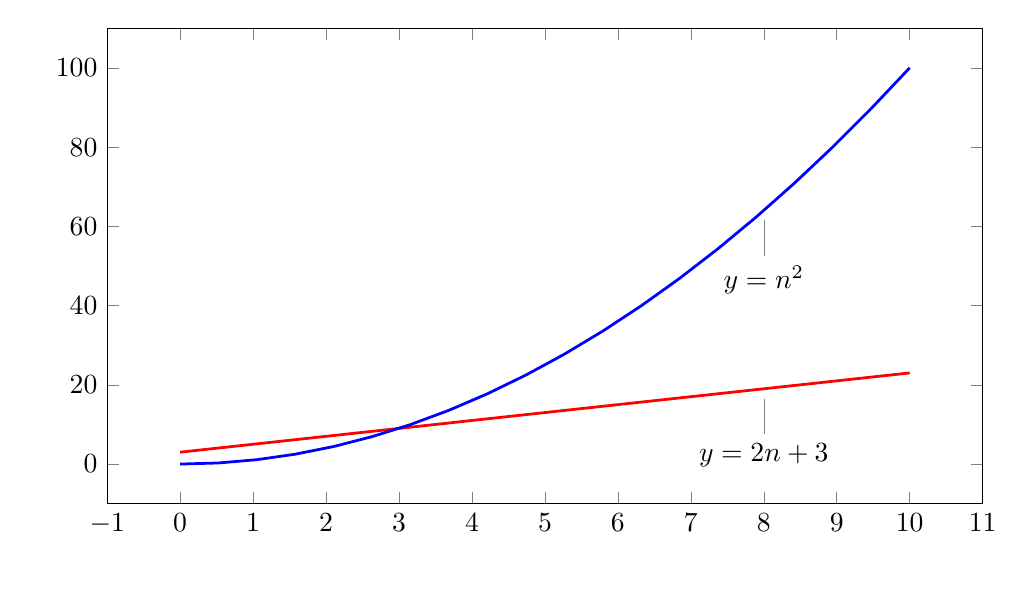
\begin{tikzpicture}[line width=1]
\begin{axis}[width=5in, height=3in,
             scatter/classes={a={mark=*,draw=black}},
             xlabel={\mbox{}},
             xlabel style={name=xlabel}, 
             ylabel={\mbox{}}, 
             legend style={
                at={(xlabel.south)},
                yshift=-1ex,
                anchor=north,
                legend cell align=left,
                },
        ]
]
\addplot[draw=red, line width=1] coordinates {(0.0,3.0)
(0.101,3.202)
(0.202,3.404)
(0.303,3.6061)
(0.404,3.8081)
(0.5051,4.0101)
(0.6061,4.2121)
(0.7071,4.4141)
(0.8081,4.6162)
(0.9091,4.8182)
(1.0101,5.0202)
(1.1111,5.2222)
(1.2121,5.4242)
(1.3131,5.6263)
(1.4141,5.8283)
(1.5152,6.0303)
(1.6162,6.2323)
(1.7172,6.4343)
(1.8182,6.6364)
(1.9192,6.8384)
(2.0202,7.0404)
(2.1212,7.2424)
(2.2222,7.4444)
(2.3232,7.6465)
(2.4242,7.8485)
(2.5253,8.0505)
(2.6263,8.2525)
(2.7273,8.4545)
(2.8283,8.6566)
(2.9293,8.8586)
(3.0303,9.0606)
(3.1313,9.2626)
(3.2323,9.4646)
(3.3333,9.6667)
(3.4343,9.8687)
(3.5354,10.0707)
(3.6364,10.2727)
(3.7374,10.4747)
(3.8384,10.6768)
(3.9394,10.8788)
(4.0404,11.0808)
(4.1414,11.2828)
(4.2424,11.4848)
(4.3434,11.6869)
(4.4444,11.8889)
(4.5455,12.0909)
(4.6465,12.2929)
(4.7475,12.4949)
(4.8485,12.697)
(4.9495,12.899)
(5.0505,13.101)
(5.1515,13.303)
(5.2525,13.5051)
(5.3535,13.7071)
(5.4545,13.9091)
(5.5556,14.1111)
(5.6566,14.3131)
(5.7576,14.5152)
(5.8586,14.7172)
(5.9596,14.9192)
(6.0606,15.1212)
(6.1616,15.3232)
(6.2626,15.5253)
(6.3636,15.7273)
(6.4646,15.9293)
(6.5657,16.1313)
(6.6667,16.3333)
(6.7677,16.5354)
(6.8687,16.7374)
(6.9697,16.9394)
(7.0707,17.1414)
(7.1717,17.3434)
(7.2727,17.5455)
(7.3737,17.7475)
(7.4747,17.9495)
(7.5758,18.1515)
(7.6768,18.3535)
(7.7778,18.5556)
(7.8788,18.7576)
(7.9798,18.9596)
(8.0808,19.1616)
(8.1818,19.3636)
(8.2828,19.5657)
(8.3838,19.7677)
(8.4848,19.9697)
(8.5859,20.1717)
(8.6869,20.3737)
(8.7879,20.5758)
(8.8889,20.7778)
(8.9899,20.9798)
(9.0909,21.1818)
(9.1919,21.3838)
(9.2929,21.5859)
(9.3939,21.7879)
(9.4949,21.9899)
(9.596,22.1919)
(9.697,22.3939)
(9.798,22.596)
(9.899,22.798)
(10.0,23.0)
(10.0,23.0)};\node[pin=below:{$y=2 n+3$}] at (axis cs:8.0,19.0) {};\addplot[draw=blue, line width=1] coordinates {(0.0,0.0)
(0.5263,0.277)
(1.0526,1.108)
(1.5789,2.4931)
(2.1053,4.4321)
(2.6316,6.9252)
(3.1579,9.9723)
(3.6842,13.5734)
(4.2105,17.7285)
(4.7368,22.4377)
(5.2632,27.7008)
(5.7895,33.518)
(6.3158,39.8892)
(6.8421,46.8144)
(7.3684,54.2936)
(7.8947,62.3269)
(8.4211,70.9141)
(8.9474,80.0554)
(9.4737,89.7507)
(10.0,100.0)};\node[pin=below:{$y=n^2$}] at (axis cs:8.0,64.0) {};
\end{axis}\end{tikzpicture}\end{center}

You see that 
\[
f(n) \leq g(n) \text{ for $n \geq 3$}
\]
If I choose $C = 1$ and $N = 3$, then for $n \geq N = 3$, 
we have (from the graph):
\[
f(n) \leq Cg(n)
\]
So we say that 
\[
f(n) = O(g(n))
\]
Note that the choice of $C$ and $N$ is not unique.
You can also choose $C = 2, N = 10$.

Here's another example.

Suppose
\[
f(n) = 3n^2 + 5 + 10 n \sin (n)
\]
Here's the plot:
%-*-latex-*-

\begin{center}
\begin{tikzpicture}[line width=1]
\begin{axis}[width=5in, height=3in,
             scatter/classes={a={mark=*,draw=black}},
             xlabel={\mbox{}},
             xlabel style={name=xlabel}, 
             ylabel={\mbox{}}, 
             legend style={
                at={(xlabel.south)},
                yshift=-1ex,
                anchor=north,
                legend cell align=left,
                },
        ]
]
\addplot[draw=red, line width=1] coordinates {(0.0,5.0)
(0.2564,5.8475)
(0.5128,8.305)
(0.7692,12.1258)
(1.0256,16.9255)
(1.2821,22.2207)
(1.5385,27.4772)
(1.7949,32.1647)
(2.0513,35.8134)
(2.3077,38.0661)
(2.5641,38.7219)
(2.8205,37.7672)
(3.0769,35.3908)
(3.3333,31.9811)
(3.5897,28.1044)
(3.8462,24.4672)
(4.1026,21.8624)
(4.359,21.1062)
(4.6154,22.9685)
(4.8718,28.1029)
(5.1282,36.9833)
(5.3846,49.851)
(5.641,66.6779)
(5.8974,87.1499)
(6.1538,110.6723)
(6.4103,136.3978)
(6.6667,163.2767)
(6.9231,190.1253)
(7.1795,215.7085)
(7.4359,238.832)
(7.6923,258.4347)
(7.9487,273.6771)
(8.2051,284.0168)
(8.4615,289.266)
(8.7179,289.6245)
(8.9744,285.6866)
(9.2308,278.4177)
(9.4872,269.1034)
(9.7436,259.2725)
(10.0,250.5979)
(10.0,250.5979)};\node[pin=left:{$y=3 n^2 + 5 + 10 n   \sin(n)$}] at (axis cs:8.0,276.14865972987053) {};
\end{axis}\end{tikzpicture}\end{center}

For this example $f(n)$ is positive so $|f(n)| = f(n)$.
Let's see if we can \textit{cap} it with 
\[
g(n) = n
\]
%-*-latex-*-

\begin{center}
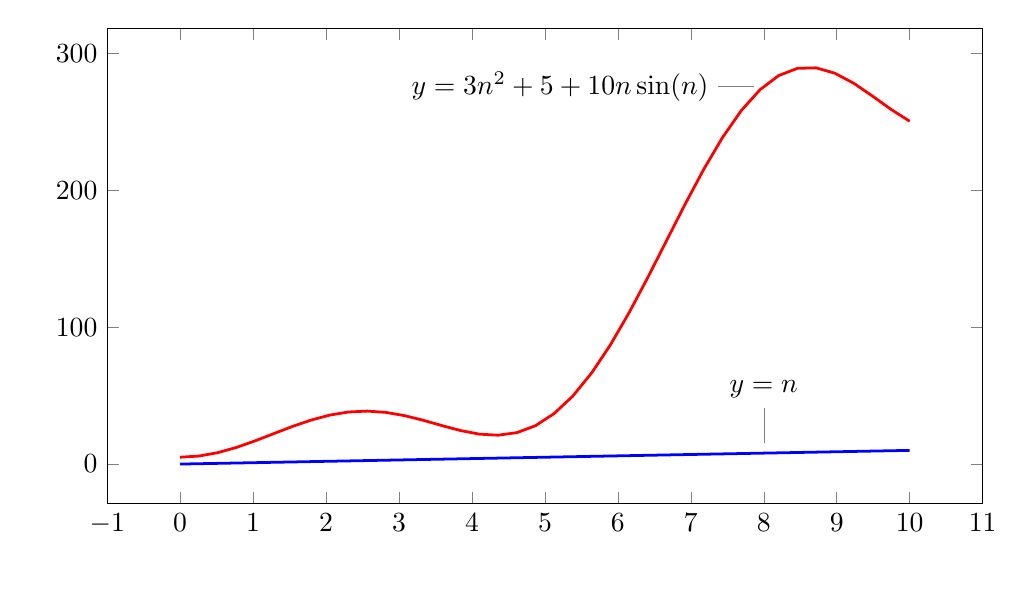
\begin{tikzpicture}[line width=1]
\begin{axis}[width=5in, height=3in,
             scatter/classes={a={mark=*,draw=black}},
             xlabel={\mbox{}},
             xlabel style={name=xlabel}, 
             ylabel={\mbox{}}, 
             legend style={
                at={(xlabel.south)},
                yshift=-1ex,
                anchor=north,
                legend cell align=left,
                },
        ]
]
\addplot[draw=red, line width=1] coordinates {(0.0,5.0)
(0.2564,5.8475)
(0.5128,8.305)
(0.7692,12.1258)
(1.0256,16.9255)
(1.2821,22.2207)
(1.5385,27.4772)
(1.7949,32.1647)
(2.0513,35.8134)
(2.3077,38.0661)
(2.5641,38.7219)
(2.8205,37.7672)
(3.0769,35.3908)
(3.3333,31.9811)
(3.5897,28.1044)
(3.8462,24.4672)
(4.1026,21.8624)
(4.359,21.1062)
(4.6154,22.9685)
(4.8718,28.1029)
(5.1282,36.9833)
(5.3846,49.851)
(5.641,66.6779)
(5.8974,87.1499)
(6.1538,110.6723)
(6.4103,136.3978)
(6.6667,163.2767)
(6.9231,190.1253)
(7.1795,215.7085)
(7.4359,238.832)
(7.6923,258.4347)
(7.9487,273.6771)
(8.2051,284.0168)
(8.4615,289.266)
(8.7179,289.6245)
(8.9744,285.6866)
(9.2308,278.4177)
(9.4872,269.1034)
(9.7436,259.2725)
(10.0,250.5979)
(10.0,250.5979)};\node[pin=left:{$y=3 n^2 + 5 + 10 n   \sin(n)$}] at (axis cs:8.0,276.14865972987053) {};\addplot[draw=blue, line width=1] coordinates {(0.0,0.0)
(5.0,5.0)
(10.0,10.0)
(10.0,10.0)};\node[pin=above:{$y=n$}] at (axis cs:8.0,8.0) {};
\end{axis}\end{tikzpicture}\end{center}

Not good.
But don't forget that if we do want to say $f(n) = O(g(n))$,
then we are allowed to use multiples of $g(n)$.
So let's try
\[
10g(n) = 10 n
\]
%-*-latex-*-

\begin{center}
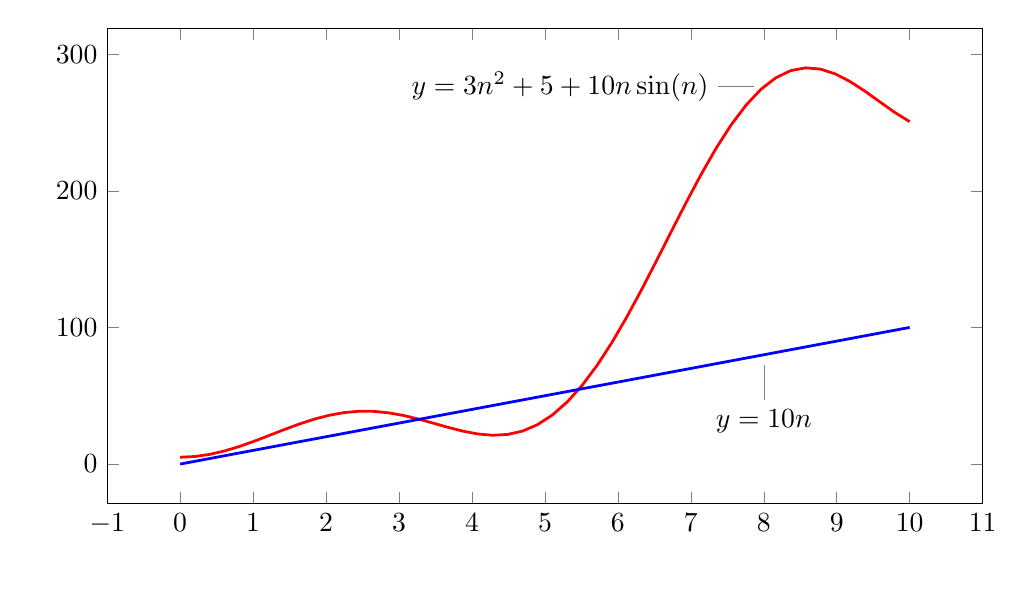
\begin{tikzpicture}[line width=1]
\begin{axis}[width=5in, height=3in,
             scatter/classes={a={mark=*,draw=black}},
             xlabel={\mbox{}},
             xlabel style={name=xlabel}, 
             ylabel={\mbox{}}, 
             legend style={
                at={(xlabel.south)},
                yshift=-1ex,
                anchor=north,
                legend cell align=left,
                },
        ]
]
\addplot[draw=red, line width=1] coordinates {(0.0,5.0)
(0.2041,5.5386)
(0.4082,7.1199)
(0.6122,9.6431)
(0.8163,12.9472)
(1.0204,16.8209)
(1.2245,21.0161)
(1.4286,25.2639)
(1.6327,29.292)
(1.8367,32.8424)
(2.0408,35.6899)
(2.2449,37.6574)
(2.449,38.6305)
(2.6531,38.5678)
(2.8571,37.5078)
(3.0612,35.5709)
(3.2653,32.9573)
(3.4694,29.94)
(3.6735,26.8531)
(3.8776,24.0763)
(4.0816,22.0167)
(4.2857,21.0872)
(4.4898,21.6846)
(4.6939,24.1667)
(4.898,28.8313)
(5.102,35.8965)
(5.3061,45.4846)
(5.5102,57.6108)
(5.7143,72.176)
(5.9184,88.9657)
(6.1224,107.6545)
(6.3265,127.8164)
(6.5306,148.9408)
(6.7347,170.4534)
(6.9388,191.7405)
(7.1429,212.1775)
(7.3469,231.1583)
(7.551,248.125)
(7.7551,262.597)
(7.9592,274.1976)
(8.1633,282.676)
(8.3673,287.9252)
(8.5714,289.9927)
(8.7755,289.0858)
(8.9796,285.5677)
(9.1837,279.9479)
(9.3878,272.8647)
(9.5918,265.0604)
(9.7959,257.3524)
(10.0,250.5979)
(10.0,250.5979)};\node[pin=left:{$y=3 n^2 + 5 + 10 n   \sin(n)$}] at (axis cs:8.0,276.14865972987053) {};\addplot[draw=blue, line width=1] coordinates {(0.0,0.0)
(5.0,50.0)
(10.0,100.0)
(10.0,100.0)};\node[pin=below:{$y=10 n$}] at (axis cs:8.0,80.0) {};
\end{axis}\end{tikzpicture}\end{center}


Better!!!
But just by looking at the graph,
my multiple of $g(n)$ must at least 
overcome the bump of $f(n)$ at around $n=8.5$.
Let's try 
\[
30g(n) = 30 n
\]
%-*-latex-*-

\begin{center}
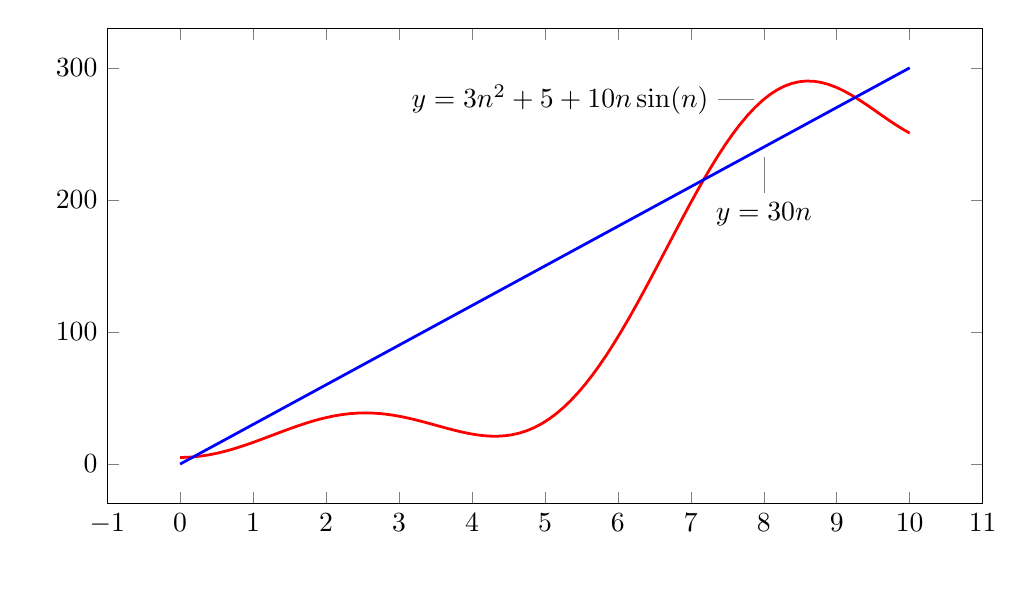
\begin{tikzpicture}[line width=1]
\begin{axis}[width=5in, height=3in,
             scatter/classes={a={mark=*,draw=black}},
             xlabel={\mbox{}},
             xlabel style={name=xlabel}, 
             ylabel={\mbox{}}, 
             legend style={
                at={(xlabel.south)},
                yshift=-1ex,
                anchor=north,
                legend cell align=left,
                },
        ]
]
\addplot[draw=red, line width=1] coordinates {(0.0,5.0)
(0.101,5.1325)
(0.202,5.5278)
(0.303,6.1798)
(0.404,7.0782)
(0.5051,8.2089)
(0.6061,9.5543)
(0.7071,11.093)
(0.8081,12.8011)
(0.9091,14.6516)
(1.0101,16.6153)
(1.1111,18.6614)
(1.2121,20.7576)
(1.3131,22.8708)
(1.4141,24.9676)
(1.5152,27.0151)
(1.6162,28.9809)
(1.7172,30.8341)
(1.8182,32.5456)
(1.9192,34.0888)
(2.0202,35.4397)
(2.1212,36.5779)
(2.2222,37.4864)
(2.3232,38.1524)
(2.4242,38.5676)
(2.5253,38.728)
(2.6263,38.6346)
(2.7273,38.2932)
(2.8283,37.7146)
(2.9293,36.9145)
(3.0303,35.9137)
(3.1313,34.7372)
(3.2323,33.4151)
(3.3333,31.9811)
(3.4343,30.4731)
(3.5354,28.9323)
(3.6364,27.4029)
(3.7374,25.9314)
(3.8384,24.5664)
(3.9394,23.3574)
(4.0404,22.3549)
(4.1414,21.6091)
(4.2424,21.1697)
(4.3434,21.0848)
(4.4444,21.4007)
(4.5455,22.1608)
(4.6465,23.4052)
(4.7475,25.17)
(4.8485,27.4869)
(4.9495,30.3823)
(5.0505,33.8773)
(5.1515,37.9868)
(5.2525,42.7194)
(5.3535,48.0772)
(5.4545,54.0555)
(5.5556,60.6425)
(5.6566,67.8195)
(5.7576,75.561)
(5.8586,83.8343)
(5.9596,92.6005)
(6.0606,101.8143)
(6.1616,111.4244)
(6.2626,121.374)
(6.3636,131.6017)
(6.4646,142.0415)
(6.5657,152.624)
(6.6667,163.2767)
(6.7677,173.9254)
(6.8687,184.4941)
(6.9697,194.907)
(7.0707,205.0882)
(7.1717,214.9636)
(7.2727,224.4613)
(7.3737,233.5124)
(7.4747,242.0521)
(7.5758,250.0206)
(7.6768,257.3637)
(7.7778,264.0335)
(7.8788,269.9895)
(7.9798,275.1987)
(8.0808,279.6366)
(8.1818,283.2871)
(8.2828,286.1436)
(8.3838,288.2087)
(8.4848,289.4945)
(8.5859,290.0229)
(8.6869,289.8253)
(8.7879,288.9424)
(8.8889,287.4242)
(8.9899,285.3294)
(9.0909,282.7249)
(9.1919,279.6854)
(9.2929,276.2927)
(9.3939,272.6348)
(9.4949,268.8049)
(9.596,264.9009)
(9.697,261.024)
(9.798,257.2779)
(9.899,253.7675)
(10.0,250.5979)
(10.0,250.5979)};\node[pin=left:{$y=3 n^2 + 5 + 10 n   \sin(n)$}] at (axis cs:8.0,276.14865972987053) {};\addplot[draw=blue, line width=1] coordinates {(0.0,0.0)
(5.0,150.0)
(10.0,300.0)
(10.0,300.0)};\node[pin=below:{$y=30 n$}] at (axis cs:8.0,240.0) {};
\end{axis}\end{tikzpicture}\end{center}


Finally let's try
\[
50g(n) = 50n
\]
%-*-latex-*-

\begin{center}
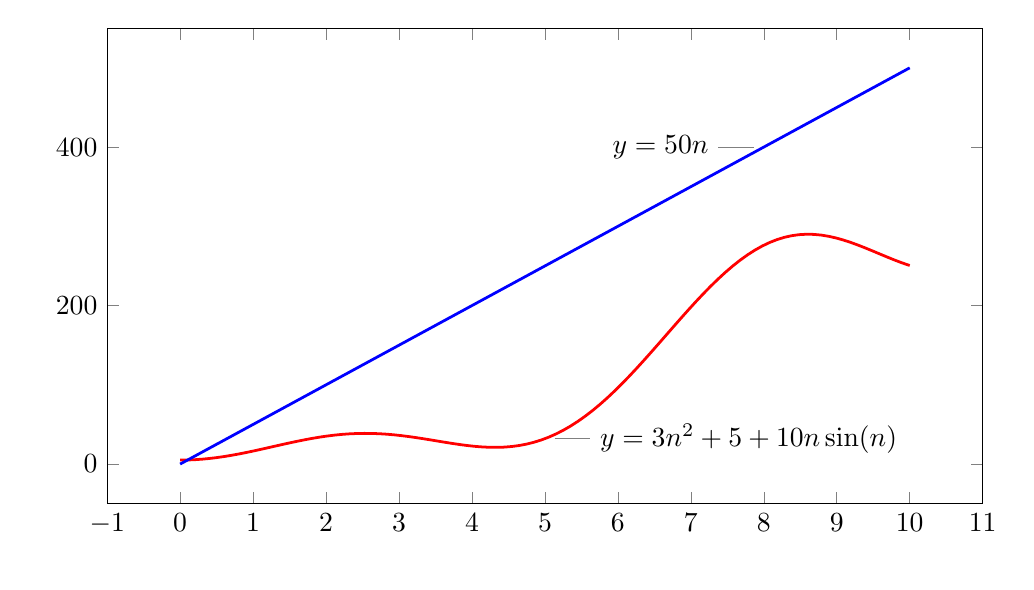
\begin{tikzpicture}[line width=1]
\begin{axis}[width=5in, height=3in,
             scatter/classes={a={mark=*,draw=black}},
             xlabel={\mbox{}},
             xlabel style={name=xlabel}, 
             ylabel={\mbox{}}, 
             legend style={
                at={(xlabel.south)},
                yshift=-1ex,
                anchor=north,
                legend cell align=left,
                },
        ]
]
\addplot[draw=red, line width=1] coordinates {(0.0,5.0)
(0.101,5.1325)
(0.202,5.5278)
(0.303,6.1798)
(0.404,7.0782)
(0.5051,8.2089)
(0.6061,9.5543)
(0.7071,11.093)
(0.8081,12.8011)
(0.9091,14.6516)
(1.0101,16.6153)
(1.1111,18.6614)
(1.2121,20.7576)
(1.3131,22.8708)
(1.4141,24.9676)
(1.5152,27.0151)
(1.6162,28.9809)
(1.7172,30.8341)
(1.8182,32.5456)
(1.9192,34.0888)
(2.0202,35.4397)
(2.1212,36.5779)
(2.2222,37.4864)
(2.3232,38.1524)
(2.4242,38.5676)
(2.5253,38.728)
(2.6263,38.6346)
(2.7273,38.2932)
(2.8283,37.7146)
(2.9293,36.9145)
(3.0303,35.9137)
(3.1313,34.7372)
(3.2323,33.4151)
(3.3333,31.9811)
(3.4343,30.4731)
(3.5354,28.9323)
(3.6364,27.4029)
(3.7374,25.9314)
(3.8384,24.5664)
(3.9394,23.3574)
(4.0404,22.3549)
(4.1414,21.6091)
(4.2424,21.1697)
(4.3434,21.0848)
(4.4444,21.4007)
(4.5455,22.1608)
(4.6465,23.4052)
(4.7475,25.17)
(4.8485,27.4869)
(4.9495,30.3823)
(5.0505,33.8773)
(5.1515,37.9868)
(5.2525,42.7194)
(5.3535,48.0772)
(5.4545,54.0555)
(5.5556,60.6425)
(5.6566,67.8195)
(5.7576,75.561)
(5.8586,83.8343)
(5.9596,92.6005)
(6.0606,101.8143)
(6.1616,111.4244)
(6.2626,121.374)
(6.3636,131.6017)
(6.4646,142.0415)
(6.5657,152.624)
(6.6667,163.2767)
(6.7677,173.9254)
(6.8687,184.4941)
(6.9697,194.907)
(7.0707,205.0882)
(7.1717,214.9636)
(7.2727,224.4613)
(7.3737,233.5124)
(7.4747,242.0521)
(7.5758,250.0206)
(7.6768,257.3637)
(7.7778,264.0335)
(7.8788,269.9895)
(7.9798,275.1987)
(8.0808,279.6366)
(8.1818,283.2871)
(8.2828,286.1436)
(8.3838,288.2087)
(8.4848,289.4945)
(8.5859,290.0229)
(8.6869,289.8253)
(8.7879,288.9424)
(8.8889,287.4242)
(8.9899,285.3294)
(9.0909,282.7249)
(9.1919,279.6854)
(9.2929,276.2927)
(9.3939,272.6348)
(9.4949,268.8049)
(9.596,264.9009)
(9.697,261.024)
(9.798,257.2779)
(9.899,253.7675)
(10.0,250.5979)
(10.0,250.5979)};\node[pin=right:{$y=3 n^2 + 5 + 10 n   \sin(n)$}] at (axis cs:5,32.053786266843076) {};\addplot[draw=blue, line width=1] coordinates {(0.0,0.0)
(5.0,250.0)
(10.0,500.0)
(10.0,500.0)};\node[pin=left:{$y=50 n$}] at (axis cs:8.0,400.0) {};
\end{axis}\end{tikzpicture}\end{center}


The picture is not that clear for small $n$ values.
So let's zoom in near $n = 0$ and see how $50n$ performs
against $f(n)$:
%-*-latex-*-

\begin{center}
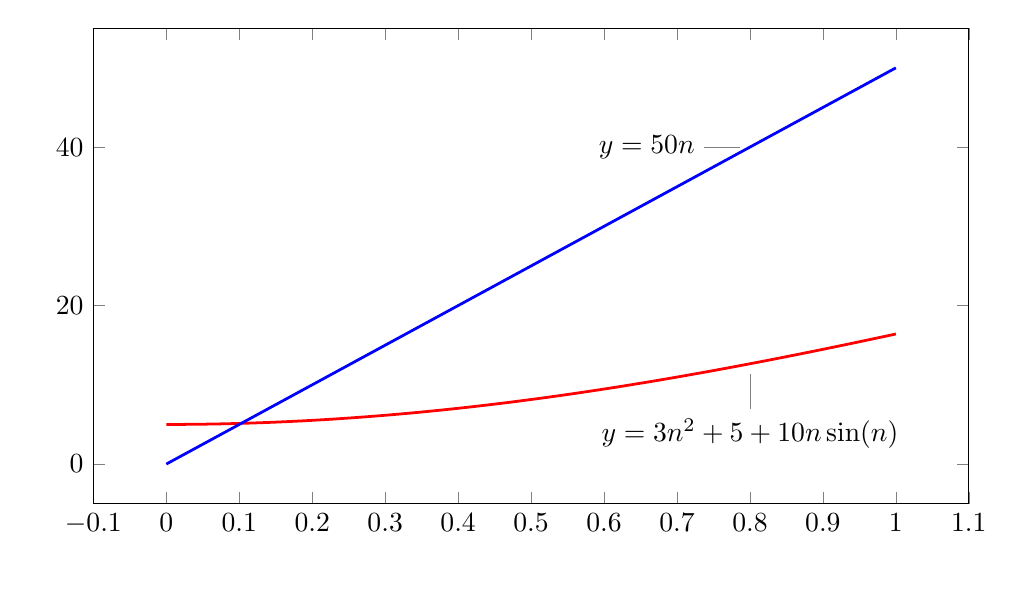
\begin{tikzpicture}[line width=1]
\begin{axis}[width=5in, height=3in,
             scatter/classes={a={mark=*,draw=black}},
             xlabel={\mbox{}},
             xlabel style={name=xlabel}, 
             ylabel={\mbox{}}, 
             legend style={
                at={(xlabel.south)},
                yshift=-1ex,
                anchor=north,
                legend cell align=left,
                },
        ]
]
\addplot[draw=red, line width=1] coordinates {(0.0,5.0)
(0.0101,5.0013)
(0.0202,5.0053)
(0.0303,5.0119)
(0.0404,5.0212)
(0.0505,5.0331)
(0.0606,5.0477)
(0.0707,5.065)
(0.0808,5.0848)
(0.0909,5.1073)
(0.101,5.1325)
(0.1111,5.1602)
(0.1212,5.1906)
(0.1313,5.2237)
(0.1414,5.2593)
(0.1515,5.2976)
(0.1616,5.3384)
(0.1717,5.3819)
(0.1818,5.4279)
(0.1919,5.4766)
(0.202,5.5278)
(0.2121,5.5816)
(0.2222,5.6379)
(0.2323,5.6968)
(0.2424,5.7583)
(0.2525,5.8222)
(0.2626,5.8887)
(0.2727,5.9578)
(0.2828,6.0293)
(0.2929,6.1033)
(0.303,6.1798)
(0.3131,6.2587)
(0.3232,6.3401)
(0.3333,6.424)
(0.3434,6.5103)
(0.3535,6.599)
(0.3636,6.6901)
(0.3737,6.7835)
(0.3838,6.8794)
(0.3939,6.9776)
(0.404,7.0782)
(0.4141,7.1811)
(0.4242,7.2863)
(0.4343,7.3937)
(0.4444,7.5035)
(0.4545,7.6155)
(0.4646,7.7298)
(0.4747,7.8463)
(0.4848,7.965)
(0.4949,8.0859)
(0.5051,8.2089)
(0.5152,8.3341)
(0.5253,8.4615)
(0.5354,8.5909)
(0.5455,8.7224)
(0.5556,8.856)
(0.5657,8.9917)
(0.5758,9.1293)
(0.5859,9.269)
(0.596,9.4106)
(0.6061,9.5543)
(0.6162,9.6998)
(0.6263,9.8473)
(0.6364,9.9966)
(0.6465,10.1478)
(0.6566,10.3009)
(0.6667,10.4558)
(0.6768,10.6125)
(0.6869,10.7709)
(0.697,10.9311)
(0.7071,11.093)
(0.7172,11.2567)
(0.7273,11.4219)
(0.7374,11.5889)
(0.7475,11.7574)
(0.7576,11.9275)
(0.7677,12.0992)
(0.7778,12.2725)
(0.7879,12.4472)
(0.798,12.6234)
(0.8081,12.8011)
(0.8182,12.9802)
(0.8283,13.1607)
(0.8384,13.3426)
(0.8485,13.5258)
(0.8586,13.7103)
(0.8687,13.8961)
(0.8788,14.0832)
(0.8889,14.2715)
(0.899,14.4609)
(0.9091,14.6516)
(0.9192,14.8433)
(0.9293,15.0362)
(0.9394,15.2302)
(0.9495,15.4252)
(0.9596,15.6212)
(0.9697,15.8182)
(0.9798,16.0161)
(0.9899,16.215)
(1.0,16.4147)
(1.0,16.4147)};\node[pin=below:{$y=3 n^2+5+10 n \sin(n)$}] at (axis cs:0.8,12.658848727196183) {};\addplot[draw=blue, line width=1] coordinates {(0.0,0.0)
(0.5,25.0)
(1.0,50.0)
(1.0,50.0)};\node[pin=left:{$y=50 n$}] at (axis cs:0.8,40.0) {};
\end{axis}\end{tikzpicture}\end{center}

Clearly from the plot for $0 \leq n \leq 1$, we see that
$50g(n)$ beats $f(n)$ after 0.1.

So from the previous two graphs
can we say that for $n \geq 1$, $50g(n)$ beats $f(n)$? ... i.e.,
can we say
\[
f(n) \leq 50 g(n) \text{ for $n \geq 1$}
\]
and conclude that $f(n) = O(g(n))$?

NO!!!

The problem is that our graphs cannot show \textit{all}
large values of $n$.
In fact when we plot for $n$ up to 20, we see that trend changes:
%-*-latex-*-

\begin{center}
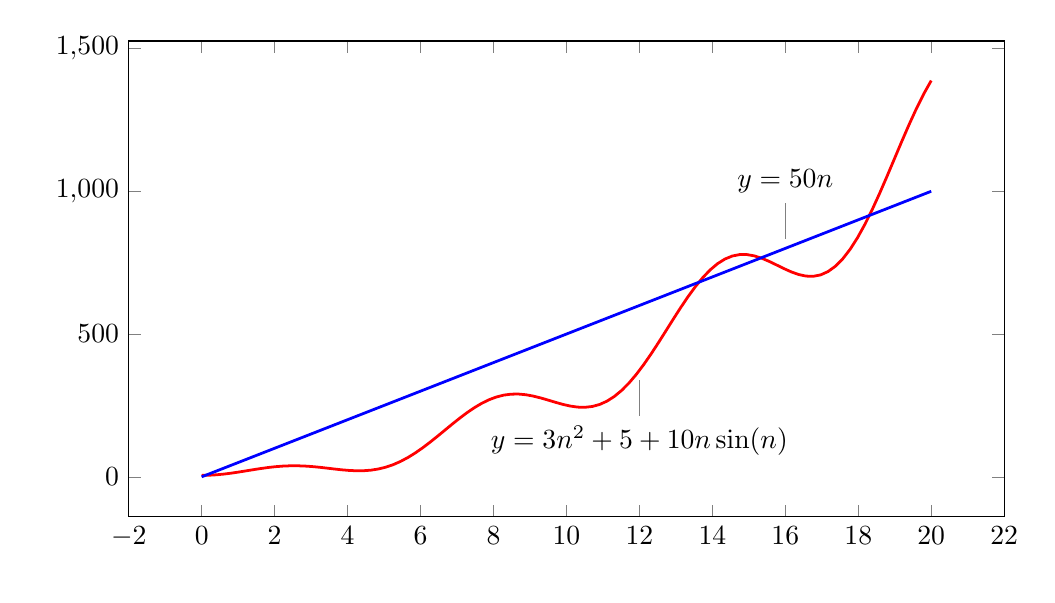
\begin{tikzpicture}[line width=1]
\begin{axis}[width=5in, height=3in,
             scatter/classes={a={mark=*,draw=black}},
             xlabel={\mbox{}},
             xlabel style={name=xlabel}, 
             ylabel={\mbox{}}, 
             legend style={
                at={(xlabel.south)},
                yshift=-1ex,
                anchor=north,
                legend cell align=left,
                },
        ]
]
\addplot[draw=red, line width=1] coordinates {(0.0,5.0)
(0.202,5.5278)
(0.404,7.0782)
(0.6061,9.5543)
(0.8081,12.8011)
(1.0101,16.6153)
(1.2121,20.7576)
(1.4141,24.9676)
(1.6162,28.9809)
(1.8182,32.5456)
(2.0202,35.4397)
(2.2222,37.4864)
(2.4242,38.5676)
(2.6263,38.6346)
(2.8283,37.7146)
(3.0303,35.9137)
(3.2323,33.4151)
(3.4343,30.4731)
(3.6364,27.4029)
(3.8384,24.5664)
(4.0404,22.3549)
(4.2424,21.1697)
(4.4444,21.4007)
(4.6465,23.4052)
(4.8485,27.4869)
(5.0505,33.8773)
(5.2525,42.7194)
(5.4545,54.0555)
(5.6566,67.8195)
(5.8586,83.8343)
(6.0606,101.8143)
(6.2626,121.374)
(6.4646,142.0415)
(6.6667,163.2767)
(6.8687,184.4941)
(7.0707,205.0882)
(7.2727,224.4613)
(7.4747,242.0521)
(7.6768,257.3637)
(7.8788,269.9895)
(8.0808,279.6366)
(8.2828,286.1436)
(8.4848,289.4945)
(8.6869,289.8253)
(8.8889,287.4242)
(9.0909,282.7249)
(9.2929,276.2927)
(9.4949,268.8049)
(9.697,261.024)
(9.899,253.7675)
(10.101,247.8732)
(10.303,244.1627)
(10.5051,243.4047)
(10.7071,246.2785)
(10.9091,253.3416)
(11.1111,265.0)
(11.3131,281.486)
(11.5152,302.8413)
(11.7172,328.9095)
(11.9192,359.3361)
(12.1212,393.5773)
(12.3232,430.918)
(12.5253,470.4972)
(12.7273,511.3406)
(12.9293,552.3998)
(13.1313,592.5949)
(13.3333,630.8602)
(13.5354,666.1907)
(13.7374,697.687)
(13.9394,724.5968)
(14.1414,746.3516)
(14.3434,762.5962)
(14.5455,773.2092)
(14.7475,778.3154)
(14.9495,778.2864)
(15.1515,773.7315)
(15.3535,765.4782)
(15.5556,754.5421)
(15.7576,742.0891)
(15.9596,729.389)
(16.1616,717.7649)
(16.3636,708.5379)
(16.5657,702.971)
(16.7677,702.2147)
(16.9697,707.2553)
(17.1717,718.8693)
(17.3737,737.5859)
(17.5758,763.659)
(17.7778,797.0499)
(17.9798,837.4227)
(18.1818,884.1517)
(18.3838,936.3413)
(18.5859,992.858)
(18.7879,1052.3727)
(18.9899,1113.4124)
(19.1919,1174.4193)
(19.3939,1233.8141)
(19.596,1290.062)
(19.798,1341.7381)
(20.0,1387.5891)
(20.0,1387.5891)};\node[pin=below:{$y=3 n^2 + 5 + 10 n   \sin(n)$}] at (axis cs:12,372.6112498399478) {};\addplot[draw=blue, line width=1] coordinates {(0.0,0.0)
(10.0,500.0)
(20.0,1000.0)
(20.0,1000.0)};\node[pin=above:{$y=50 n$}] at (axis cs:16.0,800.0) {};
\end{axis}\end{tikzpicture}\end{center}


It's even more revealing when I plot up to $n = 100$:
%-*-latex-*-

\begin{center}
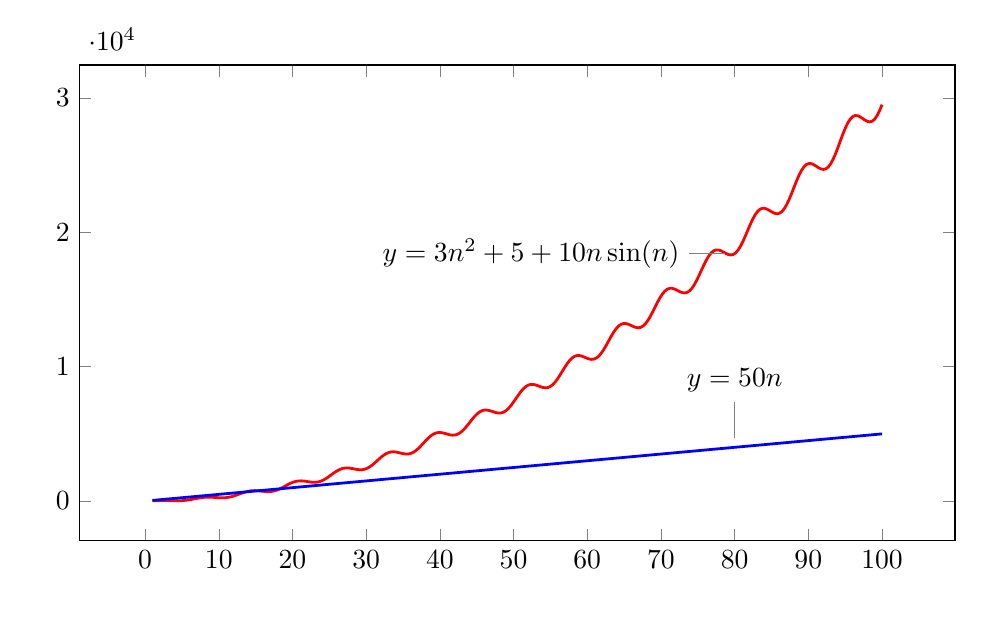
\begin{tikzpicture}[line width=1]
\begin{axis}[width=5in, height=3in,
             scatter/classes={a={mark=*,draw=black}},
             xlabel={\mbox{}},
             xlabel style={name=xlabel}, 
             ylabel={\mbox{}}, 
             legend style={
                at={(xlabel.south)},
                yshift=-1ex,
                anchor=north,
                legend cell align=left,
                },
        ]
]
\addplot[draw=red, line width=1] coordinates {(1.0,16.4147)
(1.3311,23.246)
(1.6622,29.8415)
(1.9933,35.1001)
(2.3244,38.1588)
(2.6555,38.5608)
(2.9866,36.3696)
(3.3177,32.2085)
(3.6488,27.2172)
(3.9799,22.9274)
(4.311,21.0706)
(4.6421,23.3415)
(4.9732,31.1495)
(5.3043,45.3902)
(5.6355,66.2717)
(5.9666,93.2215)
(6.2977,124.893)
(6.6288,159.2757)
(6.9599,193.9025)
(7.291,226.1309)
(7.6221,253.4683)
(7.9532,273.8999)
(8.2843,286.1789)
(8.6154,290.0386)
(8.9465,286.2962)
(9.2776,276.8272)
(9.6087,264.4085)
(9.9398,252.44)
(10.2709,244.5743)
(10.602,244.2931)
(10.9331,254.4808)
(11.2642,277.0456)
(11.5953,312.6371)
(11.9264,360.4994)
(12.2575,418.4829)
(12.5886,483.2225)
(12.9197,550.4677)
(13.2508,615.5336)
(13.5819,673.824)
(13.913,721.369)
(14.2441,755.3143)
(14.5753,774.3023)
(14.9064,778.6968)
(15.2375,770.6174)
(15.5686,753.7729)
(15.8997,733.1044)
(16.2308,714.2712)
(16.5619,703.0344)
(16.893,704.6039)
(17.2241,723.0234)
(17.5552,760.666)
(17.8863,817.9004)
(18.2174,892.9748)
(18.5485,982.1375)
(18.8796,1079.9888)
(19.2107,1180.0337)
(19.5418,1275.3762)
(19.8729,1359.4841)
(20.204,1426.937)
(20.5351,1474.0734)
(20.8662,1499.4602)
(21.1973,1504.125)
(21.5284,1491.5191)
(21.8595,1467.2052)
(22.1906,1438.2985)
(22.5217,1412.7166)
(22.8528,1398.3163)
(23.1839,1402.0133)
(23.5151,1428.9808)
(23.8462,1482.0218)
(24.1773,1561.1895)
(24.5084,1663.7048)
(24.8395,1784.1886)
(25.1706,1915.1916)
(25.5017,2047.9696)
(25.8328,2173.4231)
(26.1639,2283.1017)
(26.495,2370.1611)
(26.8261,2430.1658)
(27.1572,2461.642)
(27.4883,2466.3152)
(27.8194,2448.9965)
(28.1505,2417.1226)
(28.4816,2379.9931)
(28.8127,2347.7818)
(29.1438,2330.4288)
(29.4749,2336.5322)
(29.806,2372.3642)
(30.1371,2441.1239)
(30.4682,2542.5138)
(30.7993,2672.6959)
(31.1304,2824.6395)
(31.4615,2988.8304)
(31.7926,3154.2714)
(32.1237,3309.6668)
(32.4548,3444.6666)
(32.786,3551.0301)
(33.1171,3623.5801)
(33.4482,3660.8376)
(33.7793,3665.2593)
(34.1104,3643.0444)
(34.4415,3603.5238)
(34.7726,3558.1905)
(35.1037,3519.473)
(35.4348,3499.3807)
(35.7659,3508.1711)
(36.097,3553.1852)
(36.4281,3637.9833)
(36.7592,3761.8824)
(37.0903,3919.9547)
(37.4214,4103.4933)
(37.7525,4300.9046)
(38.0836,4498.9346)
(38.4147,4684.0998)
(38.7458,4844.1692)
(39.0769,4969.5328)
(39.408,5054.3051)
(39.7391,5097.0368)
(40.0702,5100.9493)
(40.4013,5073.658)
(40.7324,5026.4074)
(41.0635,4972.8934)
(41.3946,4927.796)
(41.7258,4905.1807)
(42.0569,4916.9409)
(42.388,4971.4553)
(42.7191,5072.6108)
(43.0502,5219.3046)
(43.3813,5405.4876)
(43.7124,5620.7531)
(44.0435,5851.4134)
(44.3746,6081.9549)
(44.7057,6296.7146)
(45.0368,6481.5994)
(45.3679,6625.6579)
(45.699,6722.3293)
(46.0301,6770.2294)
(46.3612,6773.3774)
(46.6923,6740.8326)
(47.0234,6685.7726)
(47.3545,6624.1044)
(47.6856,6572.7571)
(48.0167,6547.8379)
(48.3478,6562.8523)
(48.6789,6627.1857)
(49.01,6745.0173)
(49.3411,6914.7894)
(49.6722,7129.301)
(50.0033,7376.4217)
(50.3344,7640.356)
(50.6656,7903.3278)
(50.9967,8147.5034)
(51.3278,8356.9472)
(51.6589,8519.3941)
(51.99,8627.6416)
(52.3211,8680.4054)
(52.6522,8682.5357)
(52.9833,8644.5636)
(53.3144,8581.6182)
(53.6455,8511.8262)
(53.9766,8454.3625)
(54.3077,8427.3613)
(54.6388,8445.916)
(54.9699,8520.3881)
(55.301,8655.2136)
(55.6321,8848.3458)
(55.9632,9091.4011)
(56.2943,9370.5019)
(56.6254,9667.7314)
(56.9565,9963.0486)
(57.2876,10236.4584)
(57.6187,10470.2026)
(57.9498,10650.7302)
(58.2809,10770.2306)
(58.612,10827.5547)
(58.9431,10828.4167)
(59.2742,10784.8464)
(59.6054,10713.9433)
(59.9365,10636.0618)
(60.2676,10572.6185)
(60.5987,10543.7599)
(60.9298,10566.1431)
(61.2609,10651.0737)
(61.592,10803.2105)
(61.9231,11019.9828)
(62.2542,11291.7941)
(62.5853,11602.9965)
(62.9164,11933.5386)
(63.2475,12261.1127)
(63.5786,12563.5719)
(63.9097,12821.3553)
(64.2408,13019.6548)
(64.5719,13150.0851)
(64.903,13211.6674)
(65.2341,13211.0126)
(65.5652,13161.6765)
(65.8963,13082.7473)
(66.2274,12996.8141)
(66.5585,12927.5314)
(66.8896,12897.0429)
(67.2207,12923.5443)
(67.5518,13019.2541)
(67.8829,13189.0188)
(68.214,13429.7094)
(68.5452,13730.4861)
(68.8763,14073.908)
(69.2074,14437.7763)
(69.5385,14797.5151)
(69.8696,15128.8358)
(70.2007,15410.3952)
(70.5318,15626.1567)
(70.8629,15767.1939)
(71.194,15832.7334)
(71.5251,15830.316)
(71.8562,15775.0498)
(72.1873,15688.0295)
(72.5184,15594.0863)
(72.8495,15519.108)
(73.1806,15487.2196)
(73.5117,15518.1305)
(73.8428,15624.9407)
(74.1739,15812.6491)
(74.505,16077.5342)
(74.8361,16407.4829)
(75.1672,16783.2388)
(75.4983,17180.4432)
(75.8294,17572.251)
(76.1605,17932.2422)
(76.4916,18237.3121)
(76.8227,18470.2244)
(77.1538,18621.5457)
(77.4849,18690.7431)
(77.8161,18686.3194)
(78.1472,18624.9619)
(78.4783,18529.7894)
(78.8094,18427.8816)
(79.1405,18347.3547)
(79.4716,18314.2992)
(79.8027,18349.9128)
(80.1338,18468.145)
(80.4649,18674.1121)
(80.796,18963.4661)
(81.1271,19322.7904)
(81.4582,19730.9913)
(81.7893,20161.5379)
(82.1204,20585.3153)
(82.4515,20973.7829)
(82.7826,21302.0956)
(83.1137,21551.8467)
(83.4448,21713.1294)
(83.7759,21785.6865)
(84.107,21779.0155)
(84.4381,21711.4088)
(84.7692,21608.0267)
(85.1003,21498.2034)
(85.4314,21412.2784)
(85.7625,21378.291)
(86.0936,21418.9022)
(86.4247,21548.8782)
(86.7559,21773.4185)
(87.087,22087.5136)
(87.4181,22476.4144)
(87.7492,22917.1677)
(88.0803,23381.0589)
(88.4114,23836.7028)
(88.7425,24253.4496)
(89.0736,24604.7354)
(89.4047,24871.0121)
(89.7358,25041.9337)
(90.0669,25117.5539)
(90.398,25108.3969)
(90.7291,25034.3866)
(91.0602,24922.7409)
(91.3913,24805.0551)
(91.7224,24713.8858)
(92.0535,24679.2047)
(92.3846,24725.1096)
(92.7157,24867.152)
(93.0468,25110.5787)
(93.3779,25449.6853)
(93.709,25868.3606)
(94.0401,26341.7701)
(94.3712,26839.0043)
(94.7023,27326.4083)
(95.0334,27771.2343)
(95.3645,28145.2211)
(95.6957,28427.7092)
(96.0268,28607.9477)
(96.3579,28686.3357)
(96.689,28674.4567)
(97.0201,28593.8913)
(97.3512,28473.932)
(97.6823,28348.4403)
(98.0134,28252.1838)
(98.3445,28217.0496)
(98.6756,28268.5461)
(99.0067,28422.9776)
(99.3378,28685.6033)
(99.6689,29049.9898)
(100.0,29498.6344)
(100.0,29498.6344)};\node[pin=left:{$y=3 n^2 + 5 + 10 n   \sin(n)$}] at (axis cs:80.0,18409.8890768613) {};\addplot[draw=blue, line width=1] coordinates {(1.0,50.0)
(50.5,2525.0)
(100.0,5000.0)
(100.0,5000.0)};\node[pin=above:{$y=50 n$}] at (axis cs:80.0,4000.0) {};
\end{axis}\end{tikzpicture}\end{center}


Clearly \textit{no} straight line is going to dominate $f(n)$ because
it seems that the graph of $f(n)$ \textit{bends} up (with wiggles along the way).

Here's an important advice:
\[
\text{\textit{GRAPHS ARE USEFUL TOOLS BUT THEY CAN DECEIVE!!!}}
\]

Let's see more of the graph to see if the pattern of bending
upward with wiggles persists.
Let's plot up to $n = 200$:
%-*-latex-*-

\begin{center}
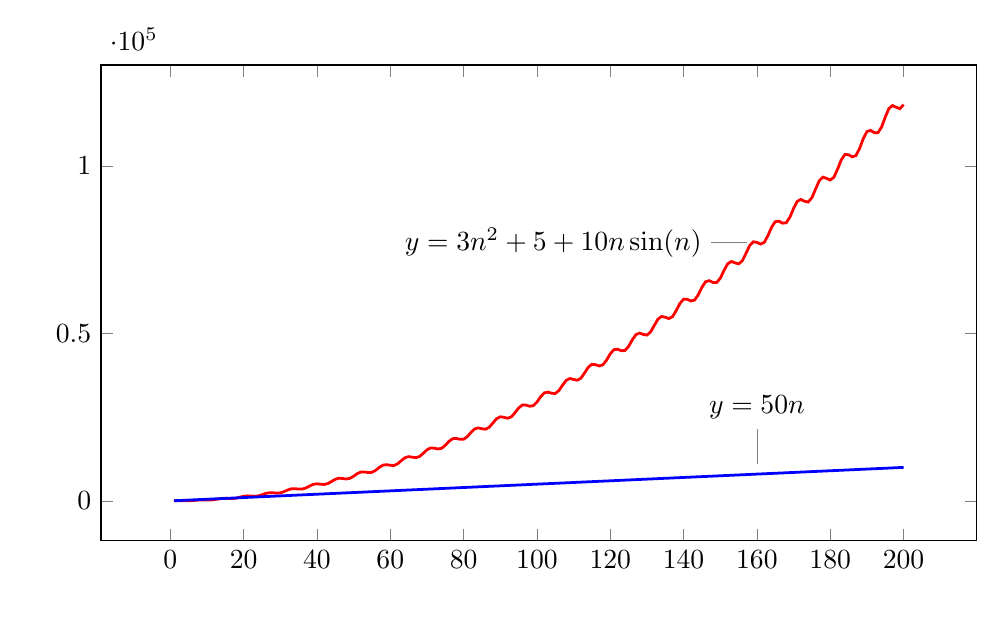
\begin{tikzpicture}[line width=1]
\begin{axis}[width=5in, height=3in,
             scatter/classes={a={mark=*,draw=black}},
             xlabel={\mbox{}},
             xlabel style={name=xlabel}, 
             ylabel={\mbox{}}, 
             legend style={
                at={(xlabel.south)},
                yshift=-1ex,
                anchor=north,
                legend cell align=left,
                },
        ]
]
\addplot[draw=red, line width=1] coordinates {(1.0,16.4147)
(2.0,35.1859)
(3.0,36.2336)
(4.0,22.7279)
(5.0,32.0538)
(6.0,96.2351)
(7.0,197.9891)
(8.0,276.1487)
(9.0,285.0907)
(10.0,250.5979)
(11.0,258.0011)
(12.0,372.6112)
(13.0,566.6217)
(14.0,731.685)
(15.0,777.5432)
(16.0,726.9355)
(17.0,708.5624)
(18.0,841.8223)
(19.0,1116.4767)
(20.0,1387.5891)
(21.0,1503.6977)
(22.0,1455.0527)
(23.0,1397.3693)
(24.0,1515.6612)
(25.0,1846.9121)
(26.0,2231.2652)
(27.0,2450.2215)
(28.0,2432.8536)
(29.0,2335.5462)
(30.0,2408.5905)
(31.0,2762.7483)
(32.0,3253.4565)
(33.0,3601.9709)
(34.0,3652.8881)
(35.0,3530.1361)
(36.0,3535.9596)
(37.0,3873.8909)
(38.0,4449.6201)
(39.0,4943.8802)
(40.0,5103.0453)
(41.0,4982.9647)
(42.0,4912.0609)
(43.0,5194.3369)
(44.0,5820.7888)
(45.0,6462.9066)
(46.0,6767.8226)
(47.0,6690.0794)
(48.0,6548.2378)
(49.0,6740.6612)
(50.0,7373.8126)
(51.0,8149.8169)
(52.0,8630.0463)
(53.0,8641.8403)
(54.0,8451.2539)
(55.0,8530.1347)
(56.0,9120.9314)
(57.0,10000.6139)
(58.0,10672.8661)
(59.0,10823.6754)
(60.0,10622.1136)
(61.0,10578.6682)
(62.0,11078.708)
(63.0,12017.4341)
(64.0,12881.8167)
(65.0,13217.4386)
(66.0,13055.4762)
(67.0,12898.8016)
(68.0,13266.4092)
(69.0,14208.7985)
(70.0,15246.7235)
(71.0,15803.2488)
(72.0,15739.7528)
(73.0,15497.9565)
(74.0,15703.9918)
(75.0,16589.1638)
(76.0,17763.2418)
(77.0,18561.6305)
(78.0,18657.9032)
(79.0,18377.151)
(80.0,18409.8891)
(81.0,19177.7907)
(82.0,20433.8476)
(83.0,21475.7425)
(84.0,21788.8799)
(85.0,21530.3357)
(86.0,21398.8257)
(87.0,21997.0185)
(88.0,23268.1505)
(89.0,24533.4618)
(90.0,25109.597)
(91.0,24944.4486)
(92.0,24679.8912)
(93.0,25070.0976)
(94.0,26282.4631)
(95.0,27729.0986)
(96.0,28597.2442)
(97.0,28600.2195)
(98.0,28255.0858)
(99.0,28418.7852)
(100.0,29498.6344)
(101.0,31064.546)
(102.0,32231.7233)
(103.0,32473.6783)
(104.0,32118.5127)
(105.0,32060.938)
(106.0,32942.2289)
(107.0,34549.7165)
(108.0,35997.964)
(109.0,36538.2494)
(110.0,36256.3331)
(111.0,36008.3479)
(112.0,36640.2049)
(113.0,38202.1844)
(114.0,39887.8776)
(115.0,40767.2506)
(116.0,40647.5272)
(117.0,40265.0534)
(118.0,40618.2964)
(119.0,42046.0291)
(120.0,43901.7334)
(121.0,45136.5664)
(122.0,45265.43)
(123.0,44826.3187)
(124.0,44898.3481)
(125.0,46109.9494)
(126.0,48048.7884)
(127.0,49627.2402)
(128.0,50079.9283)
(129.0,49678.4193)
(130.0,49495.8623)
(131.0,50424.7996)
(132.0,52347.0703)
(133.0,54227.7245)
(134.0,55060.1393)
(135.0,54799.2977)
(136.0,54418.0108)
(137.0,55020.7552)
(138.0,56822.2879)
(139.0,58935.5514)
(140.0,60177.3355)
(141.0,60160.0716)
(142.0,59662.3311)
(143.0,59924.3661)
(144.0,61505.9289)
(145.0,63758.2305)
(146.0,65407.845)
(147.0,65727.2947)
(148.0,65216.2666)
(149.0,65155.7735)
(150.0,66432.6854)
(151.0,68713.2463)
(152.0,70735.6472)
(153.0,71465.7929)
(154.0,71057.6427)
(155.0,70726.3664)
(156.0,71637.416)
(157.0,73827.1088)
(158.0,76154.4021)
(159.0,77341.8364)
(160.0,77156.0804)
(161.0,76637.1235)
(162.0,77151.9104)
(163.0,79133.4964)
(164.0,81668.6898)
(165.0,83326.3655)
(166.0,83475.264)
(167.0,82877.8312)
(168.0,83001.7489)
(169.0,84670.6202)
(170.0,87294.3041)
(171.0,89397.9704)
(172.0,89975.8937)
(173.0,89427.2978)
(174.0,89203.5562)
(175.0,90478.0145)
(176.0,93057.5239)
(177.0,95545.3339)
(178.0,96619.0841)
(179.0,96254.5927)
(180.0,95762.9253)
(181.0,96593.023)
(182.0,98993.3785)
(183.0,101768.8851)
(184.0,103369.9153)
(185.0,103321.2492)
(186.0,102673.2355)
(187.0,103047.2902)
(188.0,105143.0155)
(189.0,108081.4709)
(190.0,110200.8186)
(191.0,110584.2753)
(192.0,109915.5184)
(193.0,109863.5788)
(194.0,111550.3705)
(195.0,114507.9366)
(196.0,117094.4789)
(197.0,117999.7375)
(198.0,117459.4344)
(199.0,117053.2203)
(200.0,118258.4054)
(200.0,118258.4054)};\node[pin=left:{$y=3 n^2 + 5 + 10 n   \sin(n)$}] at (axis cs:160.0,77156.08041340641) {};\addplot[draw=blue, line width=1] coordinates {(1.0,50.0)
(100.5,5025.0)
(200.0,10000.0)
(200.0,10000.0)};\node[pin=above:{$y=50 n$}] at (axis cs:160.0,8000.0) {};
\end{axis}\end{tikzpicture}\end{center}


So let's abandon our $g(n) = n$ altogether.

What should we use to chase $f(n)$?
Of course you know that $g(n) = n^2$ is a parabola and bends up.
But does it increase (or bends) fast enough?
If you look at 
\[
f(n) = 3n^2 + 5 + 10 n \sin (n)
\]
You see that it is made up of three functions:
$3n^2$, $5$, and $10n \sin n$.
Of course $3n^2$ is going to beat $5$.
So the growth of $3n^2 + 5$ is primarily determined by $3n^2$.
Let's look at them together in a graph:
%-*-latex-*-

\begin{center}
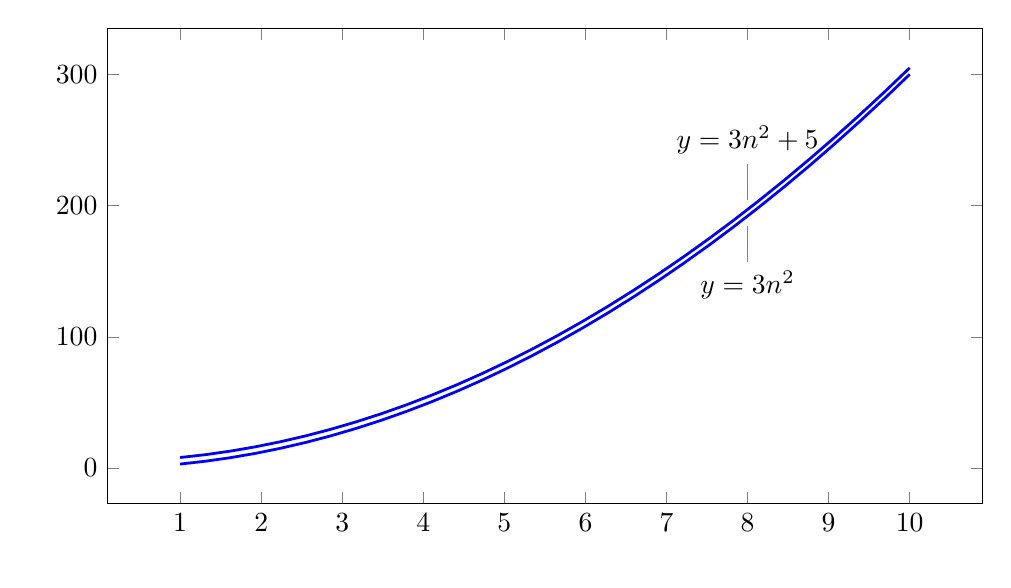
\begin{tikzpicture}[line width=1]
\begin{axis}[width=5in, height=3in,
             scatter/classes={a={mark=*,draw=black}},
             xlabel={\mbox{}},
             xlabel style={name=xlabel}, 
             ylabel={\mbox{}}, 
             legend style={
                at={(xlabel.south)},
                yshift=-1ex,
                anchor=north,
                legend cell align=left,
                },
        ]
]
\addplot[draw=blue, line width=1] coordinates {(1.0,3.0)
(1.3103,5.151)
(1.6207,7.8799)
(1.931,11.1867)
(2.2414,15.0713)
(2.5517,19.5339)
(2.8621,24.5743)
(3.1724,30.1926)
(3.4828,36.3888)
(3.7931,43.1629)
(4.1034,50.5149)
(4.4138,58.4447)
(4.7241,66.9524)
(5.0345,76.038)
(5.3448,85.7015)
(5.6552,95.9429)
(5.9655,106.7622)
(6.2759,118.1593)
(6.5862,130.1344)
(6.8966,142.6873)
(7.2069,155.8181)
(7.5172,169.5268)
(7.8276,183.8133)
(8.1379,198.6778)
(8.4483,214.1201)
(8.7586,230.1403)
(9.069,246.7384)
(9.3793,263.9144)
(9.6897,281.6683)
(10.0,300.0)};\node[pin=below:{$y=3 n^2$}] at (axis cs:8.0,192.0) {};\addplot[draw=blue, line width=1] coordinates {(1.0,8.0)
(1.3103,10.151)
(1.6207,12.8799)
(1.931,16.1867)
(2.2414,20.0713)
(2.5517,24.5339)
(2.8621,29.5743)
(3.1724,35.1926)
(3.4828,41.3888)
(3.7931,48.1629)
(4.1034,55.5149)
(4.4138,63.4447)
(4.7241,71.9524)
(5.0345,81.038)
(5.3448,90.7015)
(5.6552,100.9429)
(5.9655,111.7622)
(6.2759,123.1593)
(6.5862,135.1344)
(6.8966,147.6873)
(7.2069,160.8181)
(7.5172,174.5268)
(7.8276,188.8133)
(8.1379,203.6778)
(8.4483,219.1201)
(8.7586,235.1403)
(9.069,251.7384)
(9.3793,268.9144)
(9.6897,286.6683)
(10.0,305.0)};\node[pin=above:{$y=3 n^2 + 5$}] at (axis cs:8.0,197.0) {};
\end{axis}\end{tikzpicture}\end{center}

Of course since we can control $f(n)$ with multiples $g(n) = n^2$,
later we just need to choose a huge multiple of $n^2$ to 
beat $3n^2 + 5$, for instance $1000000 g(n) = 1000000 n^2$.

What about $10n \sin n$?
If we plot that with $3g(n) = 3n^2$ we get:
%-*-latex-*-

\begin{center}
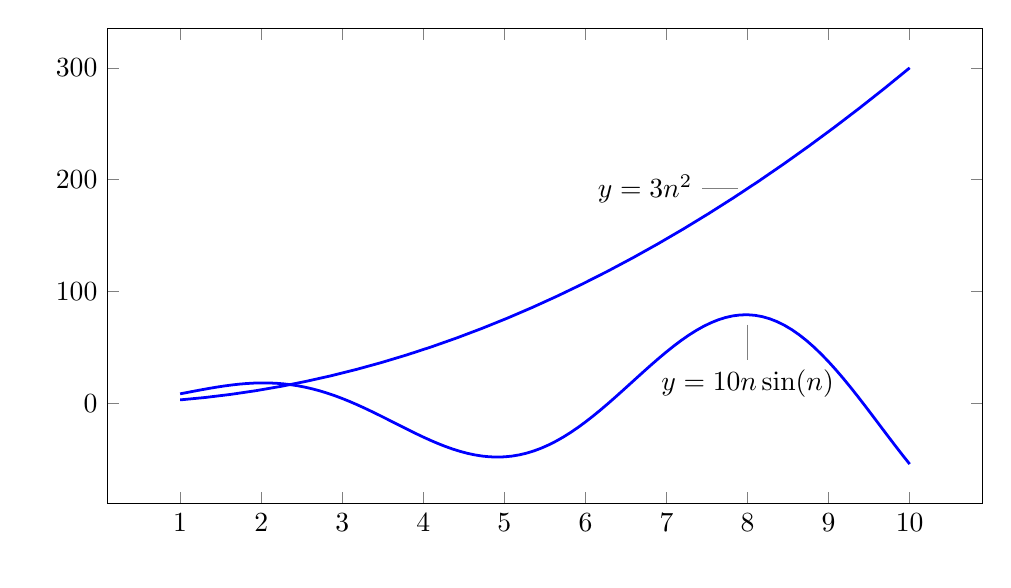
\begin{tikzpicture}[line width=1]
\begin{axis}[width=5in, height=3in,
             scatter/classes={a={mark=*,draw=black}},
             xlabel={\mbox{}},
             xlabel style={name=xlabel}, 
             ylabel={\mbox{}}, 
             legend style={
                at={(xlabel.south)},
                yshift=-1ex,
                anchor=north,
                legend cell align=left,
                },
        ]
]
\addplot[draw=blue, line width=1] coordinates {(1.0,3.0)
(1.3103,5.151)
(1.6207,7.8799)
(1.931,11.1867)
(2.2414,15.0713)
(2.5517,19.5339)
(2.8621,24.5743)
(3.1724,30.1926)
(3.4828,36.3888)
(3.7931,43.1629)
(4.1034,50.5149)
(4.4138,58.4447)
(4.7241,66.9524)
(5.0345,76.038)
(5.3448,85.7015)
(5.6552,95.9429)
(5.9655,106.7622)
(6.2759,118.1593)
(6.5862,130.1344)
(6.8966,142.6873)
(7.2069,155.8181)
(7.5172,169.5268)
(7.8276,183.8133)
(8.1379,198.6778)
(8.4483,214.1201)
(8.7586,230.1403)
(9.069,246.7384)
(9.3793,263.9144)
(9.6897,281.6683)
(10.0,300.0)};\node[pin=left:{$y=3 n^2$}] at (axis cs:8.0,192.0) {};\addplot[draw=blue, line width=1] coordinates {(1.0,8.4147)
(1.0909,9.6769)
(1.1818,10.9353)
(1.2727,12.1661)
(1.3636,13.3448)
(1.4545,14.4473)
(1.5455,15.4496)
(1.6364,16.3285)
(1.7273,17.0617)
(1.8182,17.6283)
(1.9091,18.0089)
(2.0,18.1859)
(2.0909,18.1441)
(2.1818,17.8704)
(2.2727,17.3545)
(2.3636,16.5886)
(2.4545,15.5681)
(2.5455,14.2915)
(2.6364,12.7602)
(2.7273,10.9791)
(2.8182,8.9562)
(2.9091,6.7029)
(3.0,4.2336)
(3.0909,1.5659)
(3.1818,-1.2796)
(3.2727,-4.2794)
(3.3636,-7.4075)
(3.4545,-10.6355)
(3.5455,-13.9327)
(3.6364,-17.2665)
(3.7273,-20.6031)
(3.8182,-23.9071)
(3.9091,-27.1423)
(4.0,-30.2721)
(4.0909,-33.2598)
(4.1818,-36.069)
(4.2727,-38.6637)
(4.3636,-41.0094)
(4.4545,-43.0729)
(4.5455,-44.8227)
(4.6364,-46.2297)
(4.7273,-47.2675)
(4.8182,-47.9124)
(4.9091,-48.1443)
(5.0,-47.9462)
(5.0909,-47.3054)
(5.1818,-46.2128)
(5.2727,-44.664)
(5.3636,-42.6585)
(5.4545,-40.2007)
(5.5455,-37.2993)
(5.6364,-33.9677)
(5.7273,-30.2239)
(5.8182,-26.0902)
(5.9091,-21.5936)
(6.0,-16.7649)
(6.0909,-11.6393)
(6.1818,-6.2556)
(6.2727,-0.656)
(6.3636,5.1141)
(6.4545,11.0065)
(6.5455,16.9706)
(6.6364,22.954)
(6.7273,28.9027)
(6.8182,34.7617)
(6.9091,40.4756)
(7.0,45.9891)
(7.0909,51.2471)
(7.1818,56.196)
(7.2727,60.7836)
(7.3636,64.9598)
(7.4545,68.6773)
(7.5455,71.8917)
(7.6364,74.5626)
(7.7273,76.6532)
(7.8182,78.1317)
(7.9091,78.9708)
(8.0,79.1487)
(8.0909,78.6488)
(8.1818,77.4606)
(8.2727,75.5796)
(8.3636,73.0073)
(8.4545,69.7514)
(8.5455,65.8263)
(8.6364,61.2522)
(8.7273,56.0559)
(8.8182,50.2702)
(8.9091,43.9336)
(9.0,37.0907)
(9.0909,29.791)
(9.1818,22.0893)
(9.2727,14.045)
(9.3636,5.7215)
(9.4545,-2.814)
(9.5455,-11.4912)
(9.6364,-20.2374)
(9.7273,-28.9778)
(9.8182,-37.6365)
(9.9091,-46.1368)
(10.0,-54.4021)};\node[pin=below:{$y=10   n   \sin(n)$}] at (axis cs:8.0,79.14865972987054) {};
\end{axis}\end{tikzpicture}\end{center}

To make sure that the pattern persists, I'm going to plot up
to $n = 100$:
%-*-latex-*-

\begin{center}
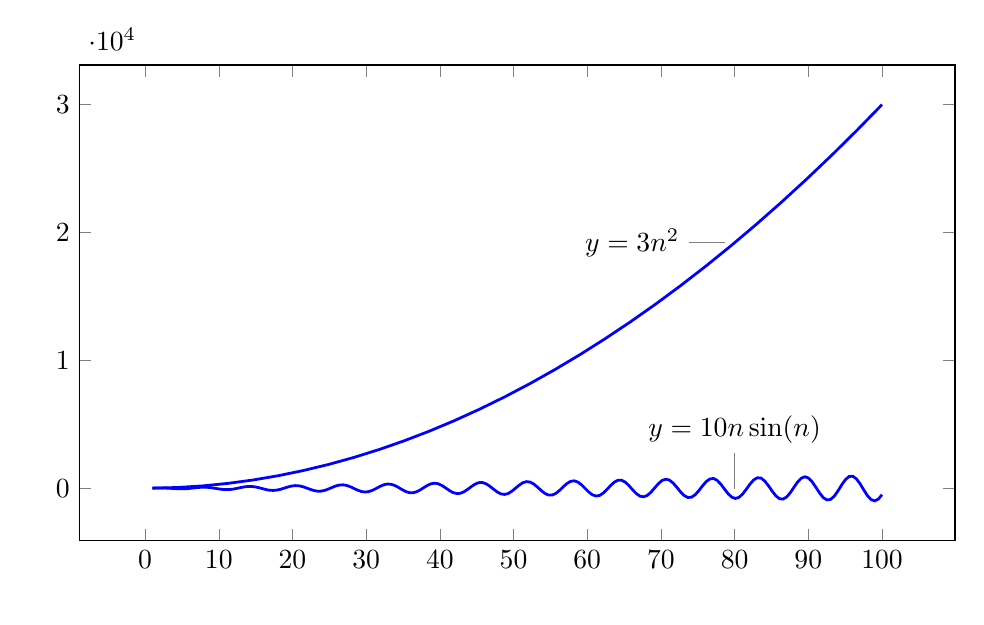
\begin{tikzpicture}[line width=1]
\begin{axis}[width=5in, height=3in,
             scatter/classes={a={mark=*,draw=black}},
             xlabel={\mbox{}},
             xlabel style={name=xlabel}, 
             ylabel={\mbox{}}, 
             legend style={
                at={(xlabel.south)},
                yshift=-1ex,
                anchor=north,
                legend cell align=left,
                },
        ]
]
\addplot[draw=blue, line width=1] coordinates {(1.0,3.0)
(4.4138,58.4447)
(7.8276,183.8133)
(11.2414,379.1058)
(14.6552,644.3222)
(18.069,979.4625)
(21.4828,1384.5268)
(24.8966,1859.5149)
(28.3103,2404.4269)
(31.7241,3019.2628)
(35.1379,3704.0226)
(38.5517,4458.7063)
(41.9655,5283.3139)
(45.3793,6177.8454)
(48.7931,7142.3008)
(52.2069,8176.6801)
(55.6207,9280.9834)
(59.0345,10455.2105)
(62.4483,11699.3615)
(65.8621,13013.4364)
(69.2759,14397.4352)
(72.6897,15851.3579)
(76.1034,17375.2045)
(79.5172,18968.975)
(82.931,20632.6694)
(86.3448,22366.2878)
(89.7586,24169.83)
(93.1724,26043.2961)
(96.5862,27986.6861)
(100.0,30000.0)
(100.0,30000.0)};\node[pin=left:{$y=3 n^2$}] at (axis cs:80.0,19200.0) {};\addplot[draw=blue, line width=1] coordinates {(1.0,8.4147)
(1.4975,14.9347)
(1.995,18.1817)
(2.4925,15.0668)
(2.9899,4.5167)
(3.4874,-11.8221)
(3.9849,-29.7619)
(4.4824,-43.644)
(4.9799,-48.0277)
(5.4774,-39.513)
(5.9749,-18.1307)
(6.4724,12.1713)
(6.9698,44.1861)
(7.4673,69.1609)
(7.9648,79.1595)
(8.4623,69.442)
(8.9598,40.1761)
(9.4573,-3.0739)
(9.9548,-50.3243)
(10.4523,-89.4714)
(10.9497,-109.3825)
(11.4472,-102.9934)
(11.9447,-69.5631)
(12.4422,-15.4085)
(12.9397,47.1932)
(13.4372,102.7749)
(13.9347,136.4996)
(14.4322,138.0875)
(14.9296,104.8182)
(15.4271,42.7564)
(15.9246,-34.233)
(16.4221,-107.5604)
(16.9196,-158.3999)
(17.4171,-172.5072)
(17.9146,-144.1387)
(18.4121,-78.0068)
(18.9095,11.3374)
(19.407,102.6727)
(19.9045,173.1462)
(20.402,203.9858)
(20.8995,185.4599)
(21.397,119.7837)
(21.8945,21.1338)
(22.392,-87.3657)
(22.8894,-179.0569)
(23.3869,-230.2969)
(23.8844,-226.5326)
(24.3819,-166.3449)
(24.8794,-62.3584)
(25.3769,61.3423)
(25.8744,174.7791)
(26.3719,249.3452)
(26.8693,265.0084)
(27.3668,215.6415)
(27.8643,111.0729)
(28.3618,-24.7779)
(28.8593,-159.3519)
(29.3568,-259.2527)
(29.8543,-298.5302)
(30.3518,-265.3913)
(30.8492,-165.6093)
(31.3467,-21.6724)
(31.8442,132.2554)
(32.3417,258.4397)
(32.8392,324.8248)
(33.3367,313.1602)
(33.8342,223.9478)
(34.3317,76.8842)
(34.8291,-93.4461)
(35.3266,-245.6963)
(35.8241,-341.7938)
(36.3216,-356.4519)
(36.8191,-283.7829)
(37.3166,-139.2908)
(37.8141,43.3748)
(38.3116,220.2419)
(38.809,347.6006)
(39.3065,392.8017)
(39.804,342.6016)
(40.3015,206.9269)
(40.799,17.0121)
(41.2965,-181.771)
(41.794,-340.7507)
(42.2915,-419.871)
(42.7889,-397.7702)
(43.2864,-277.4875)
(43.7839,-86.2889)
(44.2814,130.4839)
(44.7789,320.1607)
(45.2764,435.5402)
(45.7739,446.6284)
(46.2714,348.4001)
(46.7688,162.584)
(47.2663,-67.0996)
(47.7638,-285.2163)
(48.2613,-437.9963)
(48.7588,-486.5863)
(49.2563,-416.9084)
(49.7538,-243.6303)
(50.2513,-7.1486)
(50.7487,235.8139)
(51.2462,425.8122)
(51.7437,515.2222)
(52.2412,480.1652)
(52.7387,326.8305)
(53.2362,90.5354)
(53.7337,-172.3874)
(54.2312,-398.0153)
(54.7286,-530.377)
(55.2261,-535.3299)
(55.7236,-409.3354)
(56.2211,-180.8834)
(56.7186,95.916)
(57.2161,354.1423)
(57.7136,530.2428)
(58.2111,579.6706)
(58.7085,488.1339)
(59.206,275.6202)
(59.7035,-7.9148)
(60.201,-294.2787)
(60.6985,-513.4426)
(61.196,-610.6644)
(61.6935,-560.1509)
(62.191,-371.8495)
(62.6884,-89.5942)
(63.1859,219.081)
(63.6834,479.0978)
(64.1809,626.0945)
(64.6784,622.3506)
(65.1759,466.4367)
(65.6734,194.1276)
(66.1709,-129.7801)
(66.6683,-426.8811)
(67.1658,-624.1399)
(67.6633,-671.8419)
(68.1608,-556.1044)
(68.6583,-302.8042)
(69.1558,28.1666)
(69.6533,357.0533)
(70.1508,603.456)
(70.6482,705.9832)
(71.1457,637.5366)
(71.6432,412.4236)
(72.1407,83.4437)
(72.6382,-270.4819)
(73.1357,-563.2409)
(73.6332,-722.4816)
(74.1307,-707.4868)
(74.6281,-519.5572)
(75.1256,-202.2623)
(75.6231,168.6403)
(76.1206,503.2878)
(76.6181,719.4849)
(77.1156,762.8887)
(77.6131,620.651)
(78.1106,325.0971)
(78.608,-53.5878)
(79.1055,-424.0186)
(79.603,-695.6625)
(80.1005,-800.9641)
(80.598,-712.1349)
(81.0955,-448.4384)
(81.593,-72.0702)
(82.0905,326.4998)
(82.5879,650.2724)
(83.0854,819.3259)
(83.5829,790.5375)
(84.0804,568.5562)
(84.5779,205.2411)
(85.0754,-212.4372)
(85.5729,-583.2118)
(86.0704,-816.0724)
(86.5678,-852.6006)
(87.0653,-681.6096)
(87.5628,-342.4209)
(88.0603,84.1514)
(88.5578,495.0493)
(89.0553,789.8688)
(89.5528,895.3925)
(90.0503,783.7626)
(90.5477,479.7861)
(91.0452,55.4675)
(91.5427,-387.0374)
(92.0402,-740.0154)
(92.5377,-916.4138)
(93.0352,-871.3042)
(93.5327,-613.2986)
(94.0302,-203.0252)
(94.5276,261.104)
(95.0251,666.4969)
(95.5226,913.6946)
(96.0201,940.769)
(96.5176,738.8212)
(97.0151,354.7048)
(97.5126,-119.8227)
(98.0101,-570.0135)
(98.5075,-885.8779)
(99.005,-989.0544)
(99.5025,-852.2402)
(100.0,-506.3656)
(100.0,-506.3656)};\node[pin=above:{$y=10   n   \sin(n)$}] at (axis cs:80.0,-795.1109231387002) {};
\end{axis}\end{tikzpicture}\end{center}


At this point, we suddenly recall that the sine function
wobbles between the value of $-1$ and $1$.
Therefore $10n \sin n$ wobbles between $10n (-1)$ and $10n (+1)$,
i.e., $10n \sin n$ can be at most $10n$.
Let's check that with a plot for $n = 1$ to $n = 20$:
%-*-latex-*-

\begin{center}
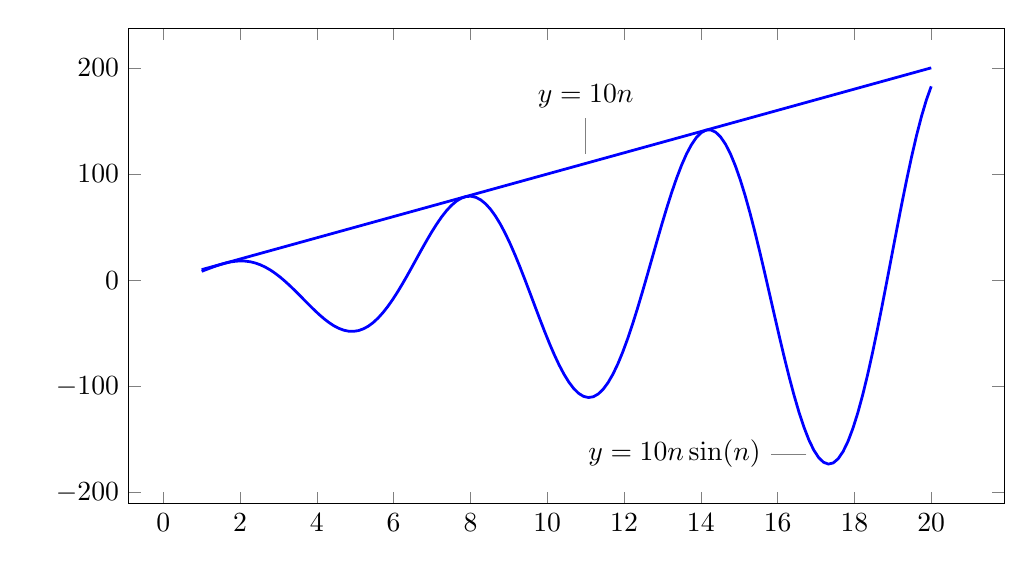
\begin{tikzpicture}[line width=1]
\begin{axis}[width=5in, height=3in,
             scatter/classes={a={mark=*,draw=black}},
             xlabel={\mbox{}},
             xlabel style={name=xlabel}, 
             ylabel={\mbox{}}, 
             legend style={
                at={(xlabel.south)},
                yshift=-1ex,
                anchor=north,
                legend cell align=left,
                },
        ]
]
\addplot[draw=blue, line width=1] coordinates {(1.0,10.0)
(10.5,105.0)
(20.0,200.0)
(20.0,200.0)};\node[pin=above:{$y=10   n$}] at (axis cs:11,110) {};\addplot[draw=blue, line width=1] coordinates {(1.0,8.4147)
(1.1275,10.1854)
(1.255,11.9298)
(1.3826,13.5813)
(1.5101,15.0728)
(1.6376,16.3393)
(1.7651,17.3189)
(1.8926,17.9545)
(2.0201,18.1961)
(2.1477,18.0012)
(2.2752,17.3372)
(2.4027,16.1816)
(2.5302,14.5235)
(2.6577,12.364)
(2.7852,9.7167)
(2.9128,6.6075)
(3.0403,3.0753)
(3.1678,-0.8296)
(3.2953,-5.0453)
(3.4228,-9.4995)
(3.5503,-14.111)
(3.6779,-18.791)
(3.8054,-23.4447)
(3.9329,-27.9732)
(4.0604,-32.2753)
(4.1879,-36.2502)
(4.3154,-39.7988)
(4.443,-42.8266)
(4.5705,-45.2452)
(4.698,-46.975)
(4.8255,-47.9467)
(4.953,-48.1031)
(5.0805,-47.4012)
(5.2081,-45.8128)
(5.3356,-43.3262)
(5.4631,-39.9468)
(5.5906,-35.6975)
(5.7181,-30.6188)
(5.8456,-24.7691)
(5.9732,-18.2234)
(6.1007,-11.0729)
(6.2282,-3.4236)
(6.3557,4.6051)
(6.4832,12.8825)
(6.6107,21.2685)
(6.7383,29.6163)
(6.8658,37.7745)
(6.9933,45.5901)
(7.1208,52.9113)
(7.2483,59.5904)
(7.3758,65.4865)
(7.5034,70.4684)
(7.6309,74.4174)
(7.7584,77.2297)
(7.8859,78.8189)
(8.0134,79.1178)
(8.1409,78.0805)
(8.2685,75.6835)
(8.396,71.9269)
(8.5235,66.835)
(8.651,60.4565)
(8.7785,52.8643)
(8.906,44.1547)
(9.0336,34.4465)
(9.1611,23.8791)
(9.2886,12.6108)
(9.4161,0.8164)
(9.5436,-11.3156)
(9.6711,-23.5858)
(9.7987,-35.7876)
(9.9262,-47.7102)
(10.0537,-59.1425)
(10.1812,-69.8766)
(10.3087,-79.712)
(10.4362,-88.4586)
(10.5638,-95.9408)
(10.6913,-102.0009)
(10.8188,-106.5018)
(10.9463,-109.3303)
(11.0738,-110.3994)
(11.2013,-109.6504)
(11.3289,-107.0546)
(11.4564,-102.6143)
(11.5839,-96.3635)
(11.7114,-88.3679)
(11.8389,-78.7245)
(11.9664,-67.5605)
(12.094,-55.0317)
(12.2215,-41.3204)
(12.349,-26.633)
(12.4765,-11.1964)
(12.604,4.7451)
(12.7315,20.9336)
(12.8591,37.1021)
(12.9866,52.9786)
(13.1141,68.291)
(13.2416,82.7713)
(13.3691,96.1607)
(13.4966,108.2139)
(13.6242,118.7037)
(13.7517,127.4251)
(13.8792,134.1992)
(14.0067,138.8769)
(14.1342,141.3417)
(14.2617,141.5122)
(14.3893,139.3445)
(14.5168,134.8331)
(14.6443,128.012)
(14.7718,118.9548)
(14.8993,107.7735)
(15.0268,94.6183)
(15.1544,79.6746)
(15.2819,63.1613)
(15.4094,45.3269)
(15.5369,26.4466)
(15.6644,6.8172)
(15.7919,-13.247)
(15.9195,-33.4192)
(16.047,-53.3658)
(16.1745,-72.7517)
(16.302,-91.2459)
(16.4295,-108.5272)
(16.557,-124.2897)
(16.6846,-138.2481)
(16.8121,-150.1432)
(16.9396,-159.7461)
(17.0671,-166.8629)
(17.1946,-171.3382)
(17.3221,-173.0585)
(17.4497,-171.9545)
(17.5772,-168.003)
(17.7047,-161.2281)
(17.8322,-151.7011)
(17.9597,-139.5401)
(18.0872,-124.9091)
(18.2148,-108.0152)
(18.3423,-89.1061)
(18.4698,-68.4666)
(18.5973,-46.4141)
(18.7248,-23.2938)
(18.8523,0.5266)
(18.9799,24.6627)
(19.1074,48.7199)
(19.2349,72.2996)
(19.3624,95.0058)
(19.4899,116.4519)
(19.6174,136.267)
(19.745,154.1027)
(19.8725,169.6388)
(20.0,182.5891)
(20.0,182.5891)};\node[pin=left:{$y=10   n   \sin(n)$}] at (axis cs:17,-163.43757361952467) {};
\end{axis}\end{tikzpicture}\end{center}


AHA!!!

This means that $3g(n) = 3n^2$ will beat $10n \sin n$ for large values of $n$.

Altogether, this means that the growth of 
\[
f(n) = 3n^2 + 5 + 10 n \sin (n)
\]
is roughly $3g(n) = 3n^2$
and therefore a higher multiple of $g(n) = n^2$ will beat
$f(n) = 3n^2 + 5 + 10 n \sin (n)$ for large values of $n$.

Here's the plot of $3g(n) = 3n^2$ and $f(n)$ for $0 \leq n \leq 10$:
%-*-latex-*-

\begin{center}
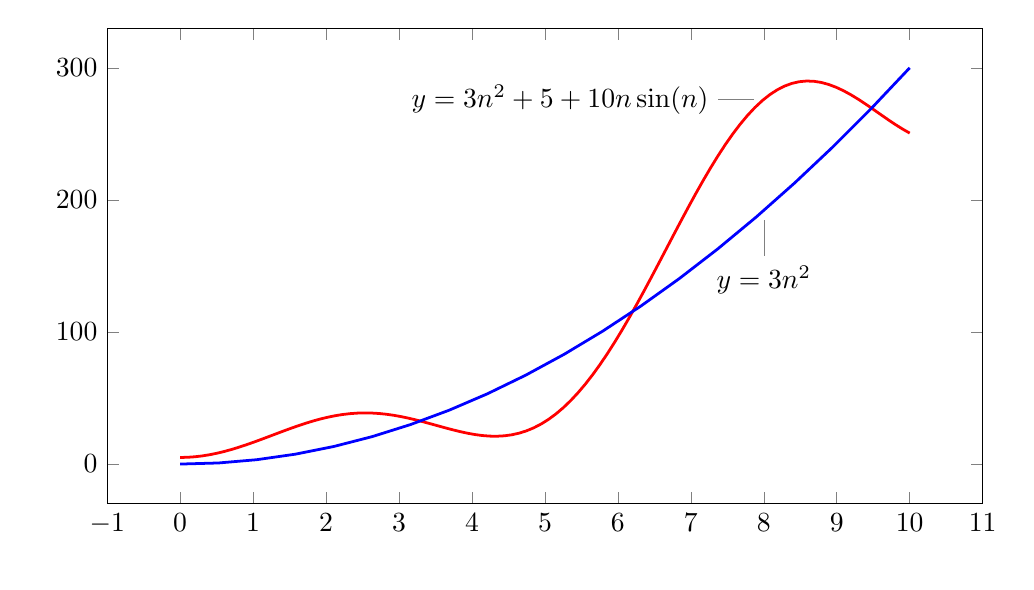
\begin{tikzpicture}[line width=1]
\begin{axis}[width=5in, height=3in,
             scatter/classes={a={mark=*,draw=black}},
             xlabel={\mbox{}},
             xlabel style={name=xlabel}, 
             ylabel={\mbox{}}, 
             legend style={
                at={(xlabel.south)},
                yshift=-1ex,
                anchor=north,
                legend cell align=left,
                },
        ]
]
\addplot[draw=red, line width=1] coordinates {(0.0,5.0)
(0.101,5.1325)
(0.202,5.5278)
(0.303,6.1798)
(0.404,7.0782)
(0.5051,8.2089)
(0.6061,9.5543)
(0.7071,11.093)
(0.8081,12.8011)
(0.9091,14.6516)
(1.0101,16.6153)
(1.1111,18.6614)
(1.2121,20.7576)
(1.3131,22.8708)
(1.4141,24.9676)
(1.5152,27.0151)
(1.6162,28.9809)
(1.7172,30.8341)
(1.8182,32.5456)
(1.9192,34.0888)
(2.0202,35.4397)
(2.1212,36.5779)
(2.2222,37.4864)
(2.3232,38.1524)
(2.4242,38.5676)
(2.5253,38.728)
(2.6263,38.6346)
(2.7273,38.2932)
(2.8283,37.7146)
(2.9293,36.9145)
(3.0303,35.9137)
(3.1313,34.7372)
(3.2323,33.4151)
(3.3333,31.9811)
(3.4343,30.4731)
(3.5354,28.9323)
(3.6364,27.4029)
(3.7374,25.9314)
(3.8384,24.5664)
(3.9394,23.3574)
(4.0404,22.3549)
(4.1414,21.6091)
(4.2424,21.1697)
(4.3434,21.0848)
(4.4444,21.4007)
(4.5455,22.1608)
(4.6465,23.4052)
(4.7475,25.17)
(4.8485,27.4869)
(4.9495,30.3823)
(5.0505,33.8773)
(5.1515,37.9868)
(5.2525,42.7194)
(5.3535,48.0772)
(5.4545,54.0555)
(5.5556,60.6425)
(5.6566,67.8195)
(5.7576,75.561)
(5.8586,83.8343)
(5.9596,92.6005)
(6.0606,101.8143)
(6.1616,111.4244)
(6.2626,121.374)
(6.3636,131.6017)
(6.4646,142.0415)
(6.5657,152.624)
(6.6667,163.2767)
(6.7677,173.9254)
(6.8687,184.4941)
(6.9697,194.907)
(7.0707,205.0882)
(7.1717,214.9636)
(7.2727,224.4613)
(7.3737,233.5124)
(7.4747,242.0521)
(7.5758,250.0206)
(7.6768,257.3637)
(7.7778,264.0335)
(7.8788,269.9895)
(7.9798,275.1987)
(8.0808,279.6366)
(8.1818,283.2871)
(8.2828,286.1436)
(8.3838,288.2087)
(8.4848,289.4945)
(8.5859,290.0229)
(8.6869,289.8253)
(8.7879,288.9424)
(8.8889,287.4242)
(8.9899,285.3294)
(9.0909,282.7249)
(9.1919,279.6854)
(9.2929,276.2927)
(9.3939,272.6348)
(9.4949,268.8049)
(9.596,264.9009)
(9.697,261.024)
(9.798,257.2779)
(9.899,253.7675)
(10.0,250.5979)
(10.0,250.5979)};\node[pin=left:{$y=3 n^2 + 5 + 10 n   \sin(n)$}] at (axis cs:8.0,276.14865972987053) {};\addplot[draw=blue, line width=1] coordinates {(0.0,0.0)
(0.5263,0.831)
(1.0526,3.3241)
(1.5789,7.4792)
(2.1053,13.2964)
(2.6316,20.7756)
(3.1579,29.9169)
(3.6842,40.7202)
(4.2105,53.1856)
(4.7368,67.313)
(5.2632,83.1025)
(5.7895,100.554)
(6.3158,119.6676)
(6.8421,140.4432)
(7.3684,162.8809)
(7.8947,186.9806)
(8.4211,212.7424)
(8.9474,240.1662)
(9.4737,269.2521)
(10.0,300.0)};\node[pin=below:{$y=3 n^2$}] at (axis cs:8.0,192.0) {};
\end{axis}\end{tikzpicture}\end{center}

It does seem like $f(n)$ winds itself around $3g(n) = 3n^2$.
To get a better feel for the pattern of things, I'm going 
to plot up to $n = 100$:
%-*-latex-*-

\begin{center}
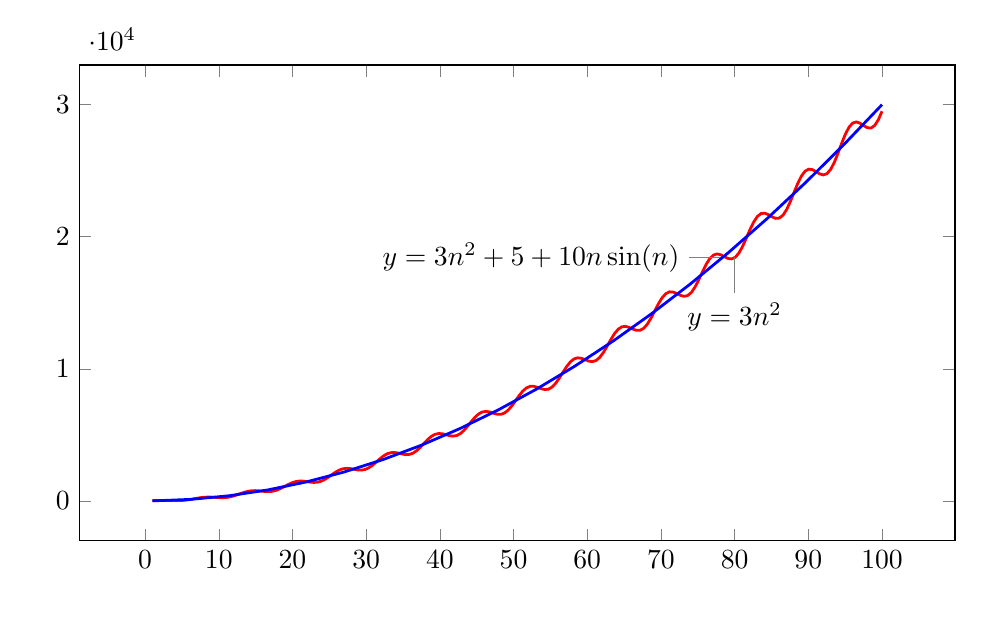
\begin{tikzpicture}[line width=1]
\begin{axis}[width=5in, height=3in,
             scatter/classes={a={mark=*,draw=black}},
             xlabel={\mbox{}},
             xlabel style={name=xlabel}, 
             ylabel={\mbox{}}, 
             legend style={
                at={(xlabel.south)},
                yshift=-1ex,
                anchor=north,
                legend cell align=left,
                },
        ]
]
\addplot[draw=red, line width=1] coordinates {(1.0,16.4147)
(1.4975,26.6621)
(1.995,35.1215)
(2.4925,38.7039)
(2.9899,36.3361)
(3.4874,29.6645)
(3.9849,22.8769)
(4.4824,21.6321)
(4.9799,31.3705)
(5.4774,55.4923)
(5.9749,93.9666)
(6.4724,142.8457)
(6.9698,194.9225)
(7.4673,241.4443)
(7.9648,274.4747)
(8.4623,289.2742)
(8.9598,286.0101)
(9.4573,270.2469)
(9.9548,251.9682)
(10.4523,243.2779)
(10.9497,255.3085)
(11.4472,295.1242)
(11.9447,363.4662)
(12.4422,454.0173)
(12.9397,554.5006)
(13.4372,649.4488)
(13.9347,724.025)
(14.4322,767.9493)
(14.9296,778.5013)
(15.4271,761.746)
(15.9246,731.5479)
(16.4221,706.4967)
(16.9196,705.4185)
(17.4171,742.5574)
(17.9146,823.6571)
(18.4121,944.0051)
(18.9095,1089.0504)
(19.407,1237.5717)
(19.9045,1366.7163)
(20.402,1457.7118)
(20.8995,1500.8269)
(21.397,1498.2766)
(21.8945,1464.2376)
(22.392,1421.8339)
(22.8894,1397.7235)
(23.3869,1415.5492)
(23.8844,1489.8643)
(24.3819,1622.0877)
(24.8794,1799.5948)
(25.3769,1998.3011)
(25.8744,2188.2285)
(26.3719,2340.7701)
(26.8693,2435.8938)
(27.3668,2467.4724)
(27.8643,2445.3342)
(28.3618,2393.3987)
(28.8593,2344.2251)
(29.3568,2331.2096)
(29.8543,2380.3023)
(30.3518,2503.2964)
(30.8492,2694.4187)
(31.3467,2931.1807)
(31.8442,3179.4187)
(32.3417,3401.3981)
(32.8392,3565.0632)
(33.3367,3652.1636)
(33.8342,3663.2011)
(34.3317,3617.8725)
(34.8291,3550.762)
(35.3266,3503.2167)
(35.8241,3513.3091)
(36.3216,3606.3257)
(36.8191,3788.1545)
(37.3166,4043.2913)
(37.8141,4338.0866)
(38.3116,4628.5682)
(38.809,4871.0266)
(39.3065,5032.8123)
(39.804,5100.6816)
(40.3015,5084.5614)
(40.799,5015.6861)
(41.2965,4939.4274)
(41.794,4904.4571)
(42.2915,4950.831)
(42.7889,5099.9112)
(43.2864,5348.6581)
(43.7839,5669.806)
(44.2814,6018.0129)
(44.7789,6340.6089)
(45.2764,6590.3925)
(45.7739,6737.3697)
(46.2714,6776.5154)
(46.7688,6729.5584)
(47.2663,6640.2187)
(47.7638,6563.931)
(48.2613,6554.4648)
(48.7588,6650.6736)
(49.2563,6866.6353)
(49.7538,7187.6822)
(50.2513,7573.4177)
(50.7487,7967.1189)
(51.2462,8309.3408)
(51.7437,8552.4595)
(52.2412,8672.596)
(52.7387,8675.9398)
(53.2362,8597.8082)
(53.7337,8494.5339)
(54.2312,8430.0395)
(54.7286,8460.2962)
(55.2261,8619.4466)
(55.7236,8911.0295)
(56.2211,9306.5547)
(56.7186,9751.9124)
(57.2161,10180.1819)
(57.7136,10527.8105)
(58.2111,10750.2515)
(58.7085,10833.2129)
(59.206,10796.6822)
(59.7035,10690.6153)
(60.201,10583.2043)
(60.6985,10544.4784)
(61.196,10629.1794)
(61.6935,10863.1008)
(62.191,11236.2951)
(62.6884,11704.9282)
(63.1859,12201.4661)
(63.6834,12650.8306)
(64.1809,12988.66)
(64.6784,13177.2337)
(65.1759,13215.1224)
(65.6734,13138.1009)
(66.1709,13010.9657)
(66.6683,12912.1223)
(67.1658,12914.6059)
(67.6633,13068.1313)
(68.1608,13386.5812)
(68.6583,13844.0787)
(69.1558,14380.7319)
(69.6533,14916.7858)
(70.1508,15371.8407)
(70.6482,15684.5052)
(71.1457,15827.6807)
(71.6432,15815.6748)
(72.1407,15701.287)
(72.6382,15563.4385)
(73.1357,15488.2414)
(73.6332,15548.0477)
(74.1307,15783.5745)
(74.6281,16193.5209)
(75.1256,16734.3177)
(75.6231,17330.2071)
(76.1206,17891.3264)
(76.6181,18335.4803)
(77.1156,18608.3257)
(77.6131,18697.0147)
(78.1106,18633.8725)
(78.608,18489.0841)
(79.1055,18354.0349)
(79.603,18319.2575)
(80.1005,18452.3074)
(80.598,18780.973)
(81.0955,19285.991)
(81.593,19905.1656)
(82.0905,20548.0268)
(82.5879,21117.5758)
(83.0854,21533.8905)
(83.5829,21753.8483)
(84.0804,21782.0982)
(84.5779,21670.4992)
(85.0754,21506.0221)
(85.5729,21389.9335)
(86.0704,21413.244)
(86.5678,21634.3717)
(87.0653,22064.5037)
(87.5628,22664.3183)
(88.0603,23353.0016)
(88.5578,24027.4953)
(89.0553,24587.3955)
(89.5528,24959.485)
(90.0503,25115.9058)
(90.5477,25081.465)
(91.0452,24928.1672)
(91.5427,24758.1678)
(92.0402,24679.1804)
(92.5377,24778.2575)
(93.0352,25100.3277)
(93.5327,25636.7788)
(94.0302,26326.9825)
(94.5276,27072.5271)
(95.0251,27760.8204)
(95.5226,28292.4034)
(96.0201,28605.3481)
(96.5176,28690.7555)
(97.0151,28595.4793)
(97.5126,28411.2771)
(98.0101,28252.8963)
(98.5075,28230.327)
(99.005,28421.9306)
(99.5025,28855.0098)
(100.0,29498.6344)
(100.0,29498.6344)};\node[pin=left:{$y=3 n^2 + 5 + 10 n   \sin(n)$}] at (axis cs:80.0,18409.8890768613) {};\addplot[draw=blue, line width=1] coordinates {(1.0,3.0)
(6.2105,115.7119)
(11.4211,391.3213)
(16.6316,829.8283)
(21.8421,1431.2327)
(27.0526,2195.5346)
(32.2632,3122.7341)
(37.4737,4212.831)
(42.6842,5465.8255)
(47.8947,6881.7175)
(53.1053,8460.5069)
(58.3158,10202.1939)
(63.5263,12106.7784)
(68.7368,14174.2604)
(73.9474,16404.6399)
(79.1579,18797.9169)
(84.3684,21354.0914)
(89.5789,24073.1634)
(94.7895,26955.133)
(100.0,30000.0)};\node[pin=below:{$y=3 n^2$}] at (axis cs:80.0,19200.0) {};
\end{axis}\end{tikzpicture}\end{center}

and then up to $n = 500$:
%-*-latex-*-

\begin{center}
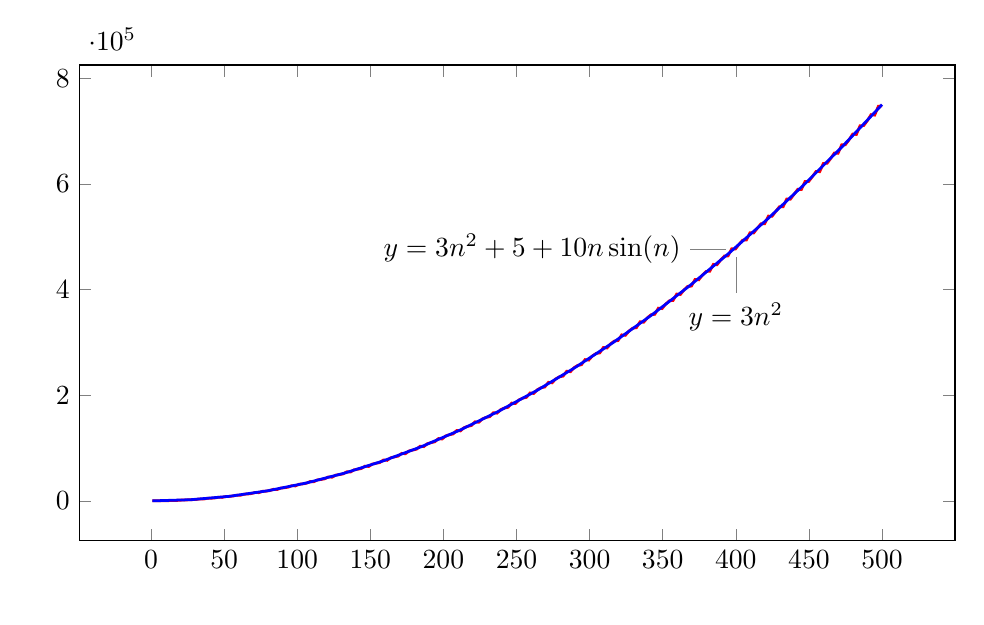
\begin{tikzpicture}[line width=1]
\begin{axis}[width=5in, height=3in,
             scatter/classes={a={mark=*,draw=black}},
             xlabel={\mbox{}},
             xlabel style={name=xlabel}, 
             ylabel={\mbox{}}, 
             legend style={
                at={(xlabel.south)},
                yshift=-1ex,
                anchor=north,
                legend cell align=left,
                },
        ]
]
\addplot[draw=red, line width=1] coordinates {(1.0,16.4147)
(3.5075,29.3574)
(6.0151,97.6089)
(8.5226,289.7793)
(11.0302,259.7571)
(13.5377,666.5782)
(16.0452,724.2533)
(18.5528,983.3568)
(21.0603,1504.5391)
(23.5678,1435.6548)
(26.0754,2255.7543)
(28.5829,2369.1408)
(31.0905,2805.4344)
(33.598,3666.6159)
(36.1055,3554.8658)
(38.6131,4783.6926)
(41.1206,4964.113)
(43.6281,5563.9419)
(46.1357,6775.7553)
(48.6432,6617.6994)
(51.1508,8250.1501)
(53.6583,8509.2517)
(56.1658,9258.9908)
(58.6734,10831.6961)
(61.1809,10624.4644)
(63.6884,12654.891)
(66.196,13004.6274)
(68.7035,13890.7034)
(71.2111,15834.1708)
(73.7186,15575.4686)
(76.2261,17997.6876)
(78.7337,18450.2989)
(81.2412,19459.2131)
(83.7487,21782.9061)
(86.2563,21471.0185)
(88.7638,24278.3198)
(91.2714,24846.3135)
(93.7789,25964.6638)
(96.2864,28677.6232)
(98.794,28311.4188)
(101.3015,31496.5763)
(103.809,32192.7066)
(106.3166,33407.2098)
(108.8241,36518.0382)
(111.3317,36096.9721)
(113.8392,39652.2543)
(116.3467,40489.502)
(118.8543,41787.0158)
(121.3618,45303.8624)
(123.8693,44827.9782)
(126.3769,48745.1598)
(128.8844,49736.7115)
(131.392,51104.2565)
(133.8995,55034.8027)
(136.407,54504.7341)
(138.9146,58775.1085)
(141.4221,59934.3354)
(143.9296,61359.1164)
(146.4372,65710.5621)
(148.9447,65127.5331)
(151.4523,69741.9251)
(153.9598,71082.3617)
(156.4673,72551.7897)
(158.9749,77330.8399)
(161.4824,76696.6648)
(163.9899,81645.4444)
(166.4975,83180.7668)
(169.005,84682.4797)
(171.5126,89895.3324)
(174.0201,89212.4146)
(176.5276,94485.5111)
(179.0352,96229.5153)
(181.5427,97751.3991)
(184.0503,103403.7331)
(186.5578,102675.0631)
(189.0653,108261.9801)
(191.5729,110228.5597)
(194.0804,111758.7692)
(196.5879,117855.7332)
(199.0955,117084.886)
(201.603,122974.7167)
(204.1106,125177.841)
(206.6181,126704.8197)
(209.1256,133251.0218)
(211.6332,132442.1535)
(214.1407,138623.597)
(216.6482,141077.2883)
(219.1558,142589.7887)
(221.6633,149589.2866)
(224.1709,148747.1301)
(226.6784,155208.5078)
(229.1859,157926.8192)
(231.6935,159413.9223)
(234.201,166870.2144)
(236.7085,166000.074)
(239.2161,172729.3471)
(241.7236,175726.3396)
(244.2312,177177.474)
(246.7387,185093.491)
(249.2462,184201.2368)
(251.7538,191186.0239)
(254.2613,194475.744)
(256.7688,195880.7045)
(259.2764,204258.8024)
(261.7839,203350.8635)
(264.2915,210578.4586)
(266.799,214174.9154)
(269.3065,215523.8817)
(271.8141,224365.8343)
(274.3216,223449.1915)
(276.8291,230906.5831)
(279.3367,234823.7259)
(281.8442,236107.2799)
(284.3518,245414.2735)
(286.8593,244496.4508)
(289.3668,252170.3409)
(291.8744,256422.0363)
(294.3819,257631.1796)
(296.8894,267403.8074)
(299.397,266492.8634)
(301.9045,274369.6873)
(304.4121,278969.6964)
(306.9196,280095.8674)
(309.4271,290334.1253)
(311.9347,289438.6432)
(314.4422,297504.5891)
(316.9497,302466.5454)
(319.4573,303501.6351)
(321.9648,314204.9182)
(324.4724,313333.9953)
(326.9799,321575.0253)
(329.4874,326912.412)
(331.995,327848.7799)
(334.5025,339015.8794)
(337.0101,338179.1161)
(339.5176,346580.9868)
(342.0251,352307.1142)
(344.5327,353137.6034)
(347.0402,364766.7049)
(349.5477,363974.1928)
(352.0553,372522.4764)
(354.5628,378650.4602)
(357.0704,379368.412)
(359.5779,391457.0941)
(362.0854,390719.403)
(364.593,399399.509)
(367.1005,405942.2481)
(369.608,406541.5156)
(372.1156,419086.7498)
(374.6231,418414.9149)
(377.1307,427212.1116)
(379.6382,434182.2664)
(382.1457,434657.228)
(384.6533,447655.3788)
(387.1608,447060.8863)
(389.6683,455960.3232)
(392.1759,463370.2938)
(394.6834,463715.8658)
(397.191,477162.6924)
(399.6985,476657.4651)
(402.206,485644.1949)
(404.7136,493506.1003)
(407.2211,493717.7487)
(409.7286,507608.4066)
(412.2362,507204.7887)
(414.7437,516263.79)
(417.2513,524589.4467)
(419.7588,524663.1984)
(422.2663,538992.2426)
(424.7739,538702.9835)
(427.2814,547819.1836)
(429.7889,556620.0851)
(432.2965,556552.5387)
(434.804,571313.9275)
(437.3116,571152.1653)
(439.8191,580310.4628)
(442.3266,589597.7595)
(444.8342,589386.0947)
(447.3417,604573.194)
(449.8492,604552.4388)
(452.3568,613737.7267)
(454.8643,623522.2056)
(457.3719,623164.1926)
(459.8794,638769.7813)
(462.3869,638903.8971)
(464.8945,648101.0861)
(467.402,658393.1515)
(469.9095,657887.1592)
(472.4171,673903.4355)
(474.9246,674206.6221)
(477.4322,683400.6637)
(479.9397,694210.318)
(482.4472,693555.3216)
(484.9548,709973.9097)
(487.4623,710460.6839)
(489.9698,719636.5937)
(492.4774,730973.4187)
(494.9849,730169.0065)
(497.4925,746980.9644)
(500.0,747666.141)
(500.0,747666.141)};\node[pin=left:{$y=3 n^2 + 5 + 10 n   \sin(n)$}] at (axis cs:400.0,476601.3225614433) {};\addplot[draw=blue, line width=1] coordinates {(1.0,3.0)
(27.2632,2229.8393)
(53.5263,8595.1994)
(79.7895,19099.0803)
(106.0526,33741.482)
(132.3158,52522.4044)
(158.5789,75441.8476)
(184.8421,102499.8116)
(211.1053,133696.2964)
(237.3684,169031.3019)
(263.6316,208504.8283)
(289.8947,252116.8753)
(316.1579,299867.4432)
(342.4211,351756.5319)
(368.6842,407784.1413)
(394.9474,467950.2715)
(421.2105,532254.9224)
(447.4737,600698.0942)
(473.7368,673279.7867)
(500.0,750000.0)
(500.0,750000.0)};\node[pin=below:{$y=3 n^2$}] at (axis cs:400.0,480000.0) {};
\end{axis}\end{tikzpicture}\end{center}


GRRREAT!!!

I see that 
$f(n) = 3n^2 + 5 + 10 n \sin (n)$
follows $3g(n)$ very tightly.
So to beat $f(n)$, let me try $4g(n) = 4n^2$
(... well ... I'm sure $(3.5)g(n)$ works too ... but I'll stick to $4g(n)$):
%-*-latex-*-

\begin{center}
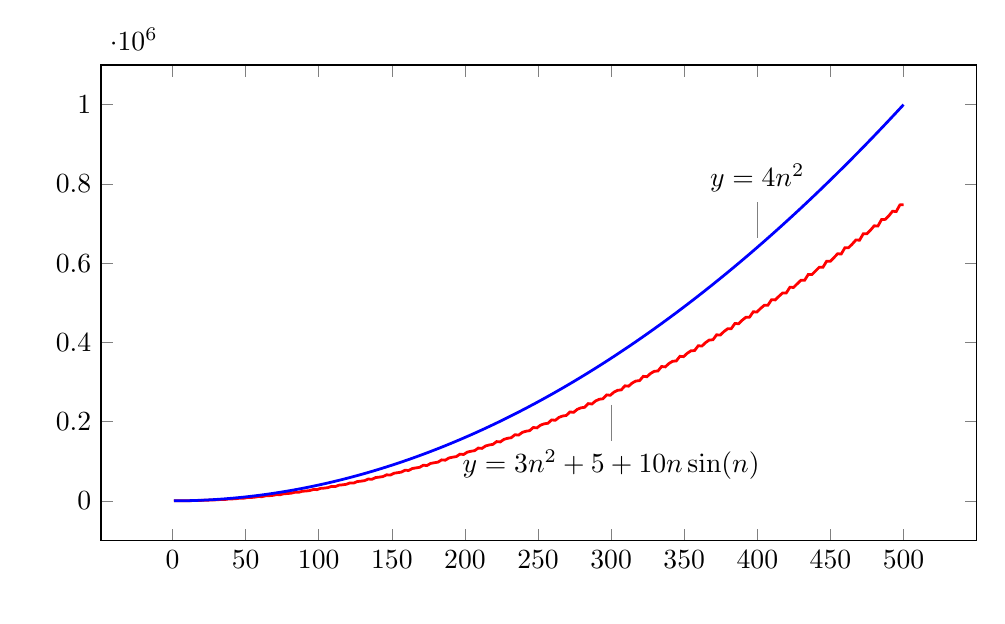
\begin{tikzpicture}[line width=1]
\begin{axis}[width=5in, height=3in,
             scatter/classes={a={mark=*,draw=black}},
             xlabel={\mbox{}},
             xlabel style={name=xlabel}, 
             ylabel={\mbox{}}, 
             legend style={
                at={(xlabel.south)},
                yshift=-1ex,
                anchor=north,
                legend cell align=left,
                },
        ]
]
\addplot[draw=red, line width=1] coordinates {(1.0,16.4147)
(3.5075,29.3574)
(6.0151,97.6089)
(8.5226,289.7793)
(11.0302,259.7571)
(13.5377,666.5782)
(16.0452,724.2533)
(18.5528,983.3568)
(21.0603,1504.5391)
(23.5678,1435.6548)
(26.0754,2255.7543)
(28.5829,2369.1408)
(31.0905,2805.4344)
(33.598,3666.6159)
(36.1055,3554.8658)
(38.6131,4783.6926)
(41.1206,4964.113)
(43.6281,5563.9419)
(46.1357,6775.7553)
(48.6432,6617.6994)
(51.1508,8250.1501)
(53.6583,8509.2517)
(56.1658,9258.9908)
(58.6734,10831.6961)
(61.1809,10624.4644)
(63.6884,12654.891)
(66.196,13004.6274)
(68.7035,13890.7034)
(71.2111,15834.1708)
(73.7186,15575.4686)
(76.2261,17997.6876)
(78.7337,18450.2989)
(81.2412,19459.2131)
(83.7487,21782.9061)
(86.2563,21471.0185)
(88.7638,24278.3198)
(91.2714,24846.3135)
(93.7789,25964.6638)
(96.2864,28677.6232)
(98.794,28311.4188)
(101.3015,31496.5763)
(103.809,32192.7066)
(106.3166,33407.2098)
(108.8241,36518.0382)
(111.3317,36096.9721)
(113.8392,39652.2543)
(116.3467,40489.502)
(118.8543,41787.0158)
(121.3618,45303.8624)
(123.8693,44827.9782)
(126.3769,48745.1598)
(128.8844,49736.7115)
(131.392,51104.2565)
(133.8995,55034.8027)
(136.407,54504.7341)
(138.9146,58775.1085)
(141.4221,59934.3354)
(143.9296,61359.1164)
(146.4372,65710.5621)
(148.9447,65127.5331)
(151.4523,69741.9251)
(153.9598,71082.3617)
(156.4673,72551.7897)
(158.9749,77330.8399)
(161.4824,76696.6648)
(163.9899,81645.4444)
(166.4975,83180.7668)
(169.005,84682.4797)
(171.5126,89895.3324)
(174.0201,89212.4146)
(176.5276,94485.5111)
(179.0352,96229.5153)
(181.5427,97751.3991)
(184.0503,103403.7331)
(186.5578,102675.0631)
(189.0653,108261.9801)
(191.5729,110228.5597)
(194.0804,111758.7692)
(196.5879,117855.7332)
(199.0955,117084.886)
(201.603,122974.7167)
(204.1106,125177.841)
(206.6181,126704.8197)
(209.1256,133251.0218)
(211.6332,132442.1535)
(214.1407,138623.597)
(216.6482,141077.2883)
(219.1558,142589.7887)
(221.6633,149589.2866)
(224.1709,148747.1301)
(226.6784,155208.5078)
(229.1859,157926.8192)
(231.6935,159413.9223)
(234.201,166870.2144)
(236.7085,166000.074)
(239.2161,172729.3471)
(241.7236,175726.3396)
(244.2312,177177.474)
(246.7387,185093.491)
(249.2462,184201.2368)
(251.7538,191186.0239)
(254.2613,194475.744)
(256.7688,195880.7045)
(259.2764,204258.8024)
(261.7839,203350.8635)
(264.2915,210578.4586)
(266.799,214174.9154)
(269.3065,215523.8817)
(271.8141,224365.8343)
(274.3216,223449.1915)
(276.8291,230906.5831)
(279.3367,234823.7259)
(281.8442,236107.2799)
(284.3518,245414.2735)
(286.8593,244496.4508)
(289.3668,252170.3409)
(291.8744,256422.0363)
(294.3819,257631.1796)
(296.8894,267403.8074)
(299.397,266492.8634)
(301.9045,274369.6873)
(304.4121,278969.6964)
(306.9196,280095.8674)
(309.4271,290334.1253)
(311.9347,289438.6432)
(314.4422,297504.5891)
(316.9497,302466.5454)
(319.4573,303501.6351)
(321.9648,314204.9182)
(324.4724,313333.9953)
(326.9799,321575.0253)
(329.4874,326912.412)
(331.995,327848.7799)
(334.5025,339015.8794)
(337.0101,338179.1161)
(339.5176,346580.9868)
(342.0251,352307.1142)
(344.5327,353137.6034)
(347.0402,364766.7049)
(349.5477,363974.1928)
(352.0553,372522.4764)
(354.5628,378650.4602)
(357.0704,379368.412)
(359.5779,391457.0941)
(362.0854,390719.403)
(364.593,399399.509)
(367.1005,405942.2481)
(369.608,406541.5156)
(372.1156,419086.7498)
(374.6231,418414.9149)
(377.1307,427212.1116)
(379.6382,434182.2664)
(382.1457,434657.228)
(384.6533,447655.3788)
(387.1608,447060.8863)
(389.6683,455960.3232)
(392.1759,463370.2938)
(394.6834,463715.8658)
(397.191,477162.6924)
(399.6985,476657.4651)
(402.206,485644.1949)
(404.7136,493506.1003)
(407.2211,493717.7487)
(409.7286,507608.4066)
(412.2362,507204.7887)
(414.7437,516263.79)
(417.2513,524589.4467)
(419.7588,524663.1984)
(422.2663,538992.2426)
(424.7739,538702.9835)
(427.2814,547819.1836)
(429.7889,556620.0851)
(432.2965,556552.5387)
(434.804,571313.9275)
(437.3116,571152.1653)
(439.8191,580310.4628)
(442.3266,589597.7595)
(444.8342,589386.0947)
(447.3417,604573.194)
(449.8492,604552.4388)
(452.3568,613737.7267)
(454.8643,623522.2056)
(457.3719,623164.1926)
(459.8794,638769.7813)
(462.3869,638903.8971)
(464.8945,648101.0861)
(467.402,658393.1515)
(469.9095,657887.1592)
(472.4171,673903.4355)
(474.9246,674206.6221)
(477.4322,683400.6637)
(479.9397,694210.318)
(482.4472,693555.3216)
(484.9548,709973.9097)
(487.4623,710460.6839)
(489.9698,719636.5937)
(492.4774,730973.4187)
(494.9849,730169.0065)
(497.4925,746980.9644)
(500.0,747666.141)
(500.0,747666.141)};\node[pin=below:{$y=3 n^2 + 5 + 10 n   \sin(n)$}] at (axis cs:300,267005.7324802966) {};\addplot[draw=blue, line width=1] coordinates {(1.0,4.0)
(6.0404,145.9459)
(11.0808,491.1372)
(16.1212,1039.5739)
(21.1616,1791.256)
(26.202,2746.1835)
(31.2424,3904.3563)
(36.2828,5265.7745)
(41.3232,6830.4381)
(46.3636,8598.3471)
(51.404,10569.5015)
(56.4444,12743.9012)
(61.4848,15121.5464)
(66.5253,17702.4369)
(71.5657,20486.5728)
(76.6061,23473.9541)
(81.6465,26664.5808)
(86.6869,30058.4528)
(91.7273,33655.5702)
(96.7677,37455.9331)
(101.8081,41459.5413)
(106.8485,45666.3949)
(111.8889,50076.4938)
(116.9293,54689.8382)
(121.9697,59506.4279)
(127.0101,64526.263)
(132.0505,69749.3435)
(137.0909,75175.6694)
(142.1313,80805.2407)
(147.1717,86638.0573)
(152.2121,92674.1194)
(157.2525,98913.4268)
(162.2929,105355.9796)
(167.3333,112001.7778)
(172.3737,118850.8213)
(177.4141,125903.1103)
(182.4545,133158.6446)
(187.4949,140617.4243)
(192.5354,148279.4494)
(197.5758,156144.7199)
(202.6162,164213.2358)
(207.6566,172484.997)
(212.697,180960.0037)
(217.7374,189638.2557)
(222.7778,198519.7531)
(227.8182,207604.4959)
(232.8586,216892.484)
(237.899,226383.7176)
(242.9394,236078.1965)
(247.9798,245975.9208)
(253.0202,256076.8905)
(258.0606,266381.1056)
(263.101,276888.5661)
(268.1414,287599.2719)
(273.1818,298513.2231)
(278.2222,309630.4198)
(283.2626,320950.8617)
(288.303,332474.5491)
(293.3434,344201.4819)
(298.3838,356131.66)
(303.4242,368265.0836)
(308.4646,380601.7525)
(313.5051,393141.6668)
(318.5455,405884.8264)
(323.5859,418831.2315)
(328.6263,431980.882)
(333.6667,445333.7778)
(338.7071,458889.919)
(343.7475,472649.3056)
(348.7879,486611.9376)
(353.8283,500777.8149)
(358.8687,515146.9377)
(363.9091,529719.3058)
(368.9495,544494.9193)
(373.9899,559473.7782)
(379.0303,574655.8825)
(384.0707,590041.2321)
(389.1111,605629.8272)
(394.1515,621421.6676)
(399.1919,637416.7534)
(404.2323,653615.0846)
(409.2727,670016.6612)
(414.3131,686621.4831)
(419.3535,703429.5505)
(424.3939,720440.8632)
(429.4343,737655.4213)
(434.4747,755073.2248)
(439.5152,772694.2736)
(444.5556,790518.5679)
(449.596,808546.1075)
(454.6364,826776.8926)
(459.6768,845210.923)
(464.7172,863848.1988)
(469.7576,882688.7199)
(474.798,901732.4865)
(479.8384,920979.4984)
(484.8788,940429.7557)
(489.9192,960083.2584)
(494.9596,979940.0065)
(500.0,1000000.0)};\node[pin=above:{$y=4 n^2$}] at (axis cs:400.0,640000.0) {};
\end{axis}\end{tikzpicture}\end{center}


To see roughly when $4g(n) = 4n^2$ beats 
$f(n) = 3n^2 + 5 + 10n  \sin n$, I zoom in and plot 
the graphs for $0 \leq n \leq 30$:
%-*-latex-*-

\begin{center}
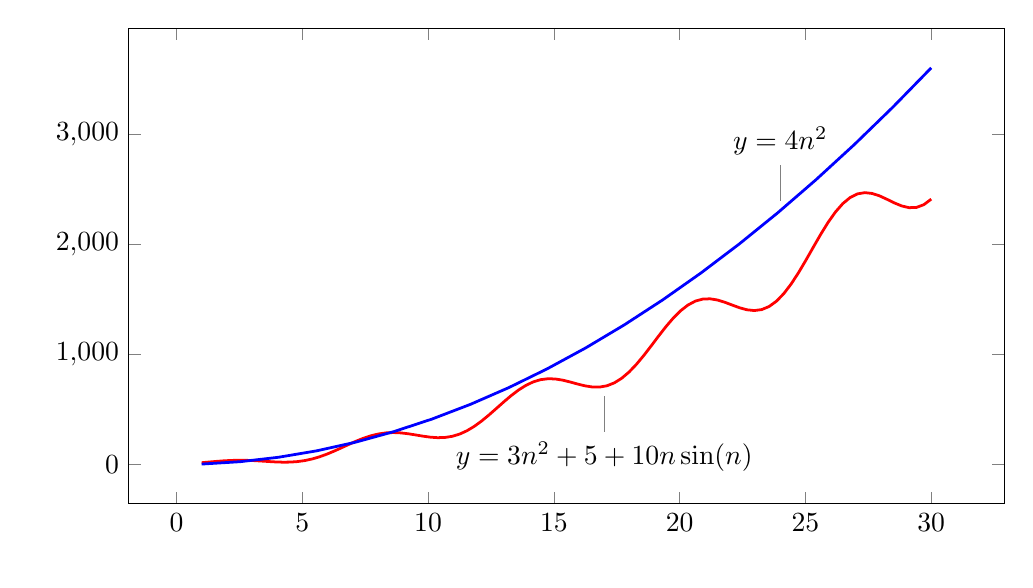
\begin{tikzpicture}[line width=1]
\begin{axis}[width=5in, height=3in,
             scatter/classes={a={mark=*,draw=black}},
             xlabel={\mbox{}},
             xlabel style={name=xlabel}, 
             ylabel={\mbox{}}, 
             legend style={
                at={(xlabel.south)},
                yshift=-1ex,
                anchor=north,
                legend cell align=left,
                },
        ]
]
\addplot[draw=red, line width=1] coordinates {(1.0,16.4147)
(1.2929,22.4484)
(1.5859,28.4016)
(1.8788,33.4933)
(2.1717,37.0617)
(2.4646,38.6624)
(2.7576,38.1439)
(3.0505,35.6915)
(3.3434,31.8329)
(3.6364,27.4029)
(3.9293,23.4698)
(4.2222,21.2307)
(4.5152,21.8837)
(4.8081,26.4921)
(5.101,35.8545)
(5.3939,50.3946)
(5.6869,70.0841)
(5.9798,94.409)
(6.2727,122.3853)
(6.5657,152.624)
(6.8586,183.443)
(7.1515,213.0165)
(7.4444,239.5475)
(7.7374,261.4491)
(8.0303,277.5153)
(8.3232,287.0641)
(8.6162,290.0382)
(8.9091,287.0493)
(9.202,279.3606)
(9.4949,268.8049)
(9.7879,257.6437)
(10.0808,248.3776)
(10.3737,243.5245)
(10.6667,245.3845)
(10.9596,255.8132)
(11.2525,276.027)
(11.5455,306.4575)
(11.8384,346.6732)
(12.1313,395.3773)
(12.4242,450.4864)
(12.7172,509.2844)
(13.0101,568.6421)
(13.303,625.2839)
(13.596,676.0796)
(13.8889,718.3338)
(14.1818,750.0487)
(14.4747,770.1327)
(14.7677,778.5354)
(15.0606,776.2931)
(15.3535,765.4782)
(15.6465,749.0519)
(15.9394,730.6326)
(16.2323,714.1964)
(16.5253,703.7343)
(16.8182,702.8971)
(17.1111,714.6583)
(17.404,741.0255)
(17.697,782.8302)
(17.9899,839.6146)
(18.2828,909.6296)
(18.5758,989.9493)
(18.8687,1076.6916)
(19.1616,1165.3326)
(19.4545,1251.0864)
(19.7475,1329.3198)
(20.0404,1395.9654)
(20.3333,1447.8973)
(20.6263,1483.2335)
(20.9192,1501.5372)
(21.2121,1503.896)
(21.5051,1492.8688)
(21.798,1472.3013)
(22.0909,1447.0233)
(22.3838,1422.4513)
(22.6768,1404.1289)
(22.9697,1397.2441)
(23.2626,1406.1662)
(23.5556,1434.0418)
(23.8485,1482.4895)
(24.1414,1551.4195)
(24.4343,1639.0007)
(24.7273,1741.7775)
(25.0202,1854.9334)
(25.3131,1972.679)
(25.6061,2088.7345)
(25.899,2196.8663)
(26.1919,2291.4312)
(26.4848,2367.8821)
(26.7778,2423.1883)
(27.0707,2456.1332)
(27.3636,2467.4598)
(27.6566,2459.8485)
(27.9495,2437.7253)
(28.2424,2406.9141)
(28.5354,2374.1592)
(28.8283,2346.5586)
(29.1212,2330.9541)
(29.4141,2333.3321)
(29.7071,2358.2861)
(30.0,2408.5905)};\node[pin=below:{$y=3 n^2+5+10 n \sin(n)$}] at (axis cs:17,708.5624263804754) {};\addplot[draw=blue, line width=1] coordinates {(1.0,4.0)
(2.5263,25.5291)
(4.0526,65.6953)
(5.5789,124.4986)
(7.1053,201.9391)
(8.6316,298.0166)
(10.1579,412.7313)
(11.6842,546.0831)
(13.2105,698.072)
(14.7368,868.6981)
(16.2632,1057.9612)
(17.7895,1265.8615)
(19.3158,1492.3989)
(20.8421,1737.5734)
(22.3684,2001.385)
(23.8947,2283.8338)
(25.4211,2584.9197)
(26.9474,2904.6427)
(28.4737,3243.0028)
(30.0,3600.0)};\node[pin=above:{$y=4 n^2$}] at (axis cs:24.0,2304.0) {};
\end{axis}\end{tikzpicture}\end{center}

It looks like $4g(n)$ definitely beats $f(n)$ for \textit{all} $n$
such that $n \geq 10$.
(Actually I can zoom in further and see if \lq\lq $n \geq 9$''
works as well ... but I'll just use \lq\lq $n \geq 10$''.)

That's it!!!

We can now say that 
\[
3n^2 + 5 + 10 n \sin (n) \leq 4n^2 \text{ for $n \geq 10$}
\]
Therefore, if I choose $C = 4$ and $N = 10$, I can say that
\[
|f(n)| \leq C |g(n)| \text{ for $n \geq N$}
\]
(Don't forget that $f(n)$ is positive for $n \geq 0$.)
This means that I can now say
\[
f(n) = O(g(n))
\]

Now we are ready for the formal definition of big-O:

\begin{defn}
Let $f(n)$ and $g(n)$ be functions.
We write 
\[
f(n) = O(g(n)) \tinysidebar{$O$}
\]
and say that 
\lq\lq $f(n)$ is \defone{big-O} of $g(n)$"
if we can find a $C$ and an $N$ such that 
for all $n \geq N$, we have
\[
|f(n)| \leq C|g(n)|
\]
\end{defn}

So now I'm ready to give a proper presentation of my solution to
the previous problem:

\newpage
\begin{eg}
Show graphically that if 
$f(n) = 3n^2 + 5 + 10 n \sin (n)$
and $g(n) = n^2$, then
\[
f(n) = O(g(n))
\]
\end{eg}

\textit{Solution.}
Let $N = 10$ and $C = 4$.
From the following graphs:
%-*-latex-*-

\begin{center}
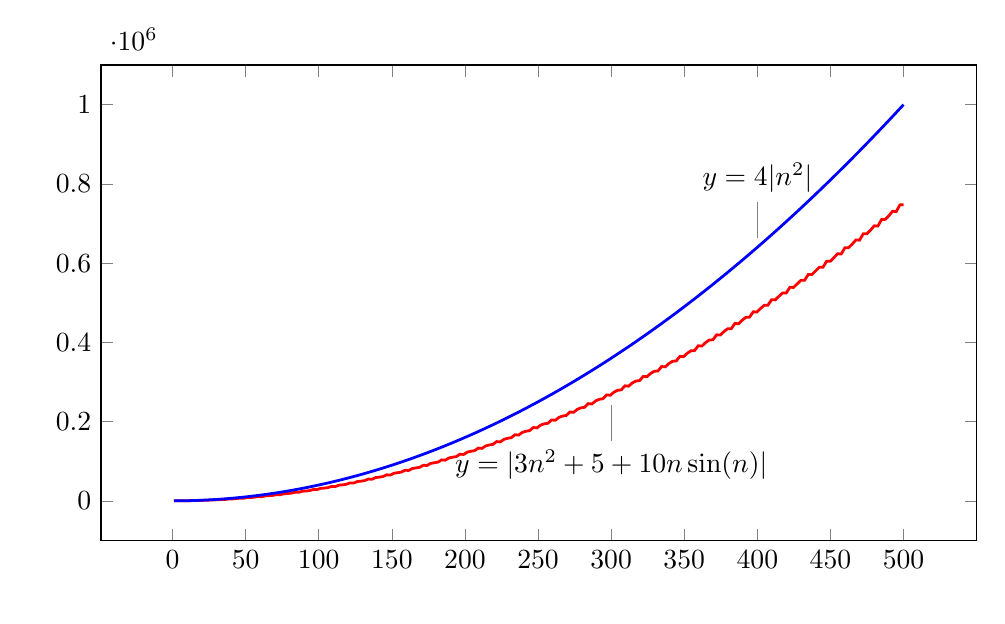
\begin{tikzpicture}[line width=1]
\begin{axis}[width=5in, height=3in,
             scatter/classes={a={mark=*,draw=black}},
             xlabel={\mbox{}},
             xlabel style={name=xlabel}, 
             ylabel={\mbox{}}, 
             legend style={
                at={(xlabel.south)},
                yshift=-1ex,
                anchor=north,
                legend cell align=left,
                },
        ]
]
\addplot[draw=red, line width=1] coordinates {(1.0,16.4147)
(3.5075,29.3574)
(6.0151,97.6089)
(8.5226,289.7793)
(11.0302,259.7571)
(13.5377,666.5782)
(16.0452,724.2533)
(18.5528,983.3568)
(21.0603,1504.5391)
(23.5678,1435.6548)
(26.0754,2255.7543)
(28.5829,2369.1408)
(31.0905,2805.4344)
(33.598,3666.6159)
(36.1055,3554.8658)
(38.6131,4783.6926)
(41.1206,4964.113)
(43.6281,5563.9419)
(46.1357,6775.7553)
(48.6432,6617.6994)
(51.1508,8250.1501)
(53.6583,8509.2517)
(56.1658,9258.9908)
(58.6734,10831.6961)
(61.1809,10624.4644)
(63.6884,12654.891)
(66.196,13004.6274)
(68.7035,13890.7034)
(71.2111,15834.1708)
(73.7186,15575.4686)
(76.2261,17997.6876)
(78.7337,18450.2989)
(81.2412,19459.2131)
(83.7487,21782.9061)
(86.2563,21471.0185)
(88.7638,24278.3198)
(91.2714,24846.3135)
(93.7789,25964.6638)
(96.2864,28677.6232)
(98.794,28311.4188)
(101.3015,31496.5763)
(103.809,32192.7066)
(106.3166,33407.2098)
(108.8241,36518.0382)
(111.3317,36096.9721)
(113.8392,39652.2543)
(116.3467,40489.502)
(118.8543,41787.0158)
(121.3618,45303.8624)
(123.8693,44827.9782)
(126.3769,48745.1598)
(128.8844,49736.7115)
(131.392,51104.2565)
(133.8995,55034.8027)
(136.407,54504.7341)
(138.9146,58775.1085)
(141.4221,59934.3354)
(143.9296,61359.1164)
(146.4372,65710.5621)
(148.9447,65127.5331)
(151.4523,69741.9251)
(153.9598,71082.3617)
(156.4673,72551.7897)
(158.9749,77330.8399)
(161.4824,76696.6648)
(163.9899,81645.4444)
(166.4975,83180.7668)
(169.005,84682.4797)
(171.5126,89895.3324)
(174.0201,89212.4146)
(176.5276,94485.5111)
(179.0352,96229.5153)
(181.5427,97751.3991)
(184.0503,103403.7331)
(186.5578,102675.0631)
(189.0653,108261.9801)
(191.5729,110228.5597)
(194.0804,111758.7692)
(196.5879,117855.7332)
(199.0955,117084.886)
(201.603,122974.7167)
(204.1106,125177.841)
(206.6181,126704.8197)
(209.1256,133251.0218)
(211.6332,132442.1535)
(214.1407,138623.597)
(216.6482,141077.2883)
(219.1558,142589.7887)
(221.6633,149589.2866)
(224.1709,148747.1301)
(226.6784,155208.5078)
(229.1859,157926.8192)
(231.6935,159413.9223)
(234.201,166870.2144)
(236.7085,166000.074)
(239.2161,172729.3471)
(241.7236,175726.3396)
(244.2312,177177.474)
(246.7387,185093.491)
(249.2462,184201.2368)
(251.7538,191186.0239)
(254.2613,194475.744)
(256.7688,195880.7045)
(259.2764,204258.8024)
(261.7839,203350.8635)
(264.2915,210578.4586)
(266.799,214174.9154)
(269.3065,215523.8817)
(271.8141,224365.8343)
(274.3216,223449.1915)
(276.8291,230906.5831)
(279.3367,234823.7259)
(281.8442,236107.2799)
(284.3518,245414.2735)
(286.8593,244496.4508)
(289.3668,252170.3409)
(291.8744,256422.0363)
(294.3819,257631.1796)
(296.8894,267403.8074)
(299.397,266492.8634)
(301.9045,274369.6873)
(304.4121,278969.6964)
(306.9196,280095.8674)
(309.4271,290334.1253)
(311.9347,289438.6432)
(314.4422,297504.5891)
(316.9497,302466.5454)
(319.4573,303501.6351)
(321.9648,314204.9182)
(324.4724,313333.9953)
(326.9799,321575.0253)
(329.4874,326912.412)
(331.995,327848.7799)
(334.5025,339015.8794)
(337.0101,338179.1161)
(339.5176,346580.9868)
(342.0251,352307.1142)
(344.5327,353137.6034)
(347.0402,364766.7049)
(349.5477,363974.1928)
(352.0553,372522.4764)
(354.5628,378650.4602)
(357.0704,379368.412)
(359.5779,391457.0941)
(362.0854,390719.403)
(364.593,399399.509)
(367.1005,405942.2481)
(369.608,406541.5156)
(372.1156,419086.7498)
(374.6231,418414.9149)
(377.1307,427212.1116)
(379.6382,434182.2664)
(382.1457,434657.228)
(384.6533,447655.3788)
(387.1608,447060.8863)
(389.6683,455960.3232)
(392.1759,463370.2938)
(394.6834,463715.8658)
(397.191,477162.6924)
(399.6985,476657.4651)
(402.206,485644.1949)
(404.7136,493506.1003)
(407.2211,493717.7487)
(409.7286,507608.4066)
(412.2362,507204.7887)
(414.7437,516263.79)
(417.2513,524589.4467)
(419.7588,524663.1984)
(422.2663,538992.2426)
(424.7739,538702.9835)
(427.2814,547819.1836)
(429.7889,556620.0851)
(432.2965,556552.5387)
(434.804,571313.9275)
(437.3116,571152.1653)
(439.8191,580310.4628)
(442.3266,589597.7595)
(444.8342,589386.0947)
(447.3417,604573.194)
(449.8492,604552.4388)
(452.3568,613737.7267)
(454.8643,623522.2056)
(457.3719,623164.1926)
(459.8794,638769.7813)
(462.3869,638903.8971)
(464.8945,648101.0861)
(467.402,658393.1515)
(469.9095,657887.1592)
(472.4171,673903.4355)
(474.9246,674206.6221)
(477.4322,683400.6637)
(479.9397,694210.318)
(482.4472,693555.3216)
(484.9548,709973.9097)
(487.4623,710460.6839)
(489.9698,719636.5937)
(492.4774,730973.4187)
(494.9849,730169.0065)
(497.4925,746980.9644)
(500.0,747666.141)
(500.0,747666.141)};\node[pin=below:{$y=|3n^2 + 5 + 10n \sin(n)|$}] at (axis cs:300,267005.7324802966) {};\addplot[draw=blue, line width=1] coordinates {(1.0,4.0)
(6.0404,145.9459)
(11.0808,491.1372)
(16.1212,1039.5739)
(21.1616,1791.256)
(26.202,2746.1835)
(31.2424,3904.3563)
(36.2828,5265.7745)
(41.3232,6830.4381)
(46.3636,8598.3471)
(51.404,10569.5015)
(56.4444,12743.9012)
(61.4848,15121.5464)
(66.5253,17702.4369)
(71.5657,20486.5728)
(76.6061,23473.9541)
(81.6465,26664.5808)
(86.6869,30058.4528)
(91.7273,33655.5702)
(96.7677,37455.9331)
(101.8081,41459.5413)
(106.8485,45666.3949)
(111.8889,50076.4938)
(116.9293,54689.8382)
(121.9697,59506.4279)
(127.0101,64526.263)
(132.0505,69749.3435)
(137.0909,75175.6694)
(142.1313,80805.2407)
(147.1717,86638.0573)
(152.2121,92674.1194)
(157.2525,98913.4268)
(162.2929,105355.9796)
(167.3333,112001.7778)
(172.3737,118850.8213)
(177.4141,125903.1103)
(182.4545,133158.6446)
(187.4949,140617.4243)
(192.5354,148279.4494)
(197.5758,156144.7199)
(202.6162,164213.2358)
(207.6566,172484.997)
(212.697,180960.0037)
(217.7374,189638.2557)
(222.7778,198519.7531)
(227.8182,207604.4959)
(232.8586,216892.484)
(237.899,226383.7176)
(242.9394,236078.1965)
(247.9798,245975.9208)
(253.0202,256076.8905)
(258.0606,266381.1056)
(263.101,276888.5661)
(268.1414,287599.2719)
(273.1818,298513.2231)
(278.2222,309630.4198)
(283.2626,320950.8617)
(288.303,332474.5491)
(293.3434,344201.4819)
(298.3838,356131.66)
(303.4242,368265.0836)
(308.4646,380601.7525)
(313.5051,393141.6668)
(318.5455,405884.8264)
(323.5859,418831.2315)
(328.6263,431980.882)
(333.6667,445333.7778)
(338.7071,458889.919)
(343.7475,472649.3056)
(348.7879,486611.9376)
(353.8283,500777.8149)
(358.8687,515146.9377)
(363.9091,529719.3058)
(368.9495,544494.9193)
(373.9899,559473.7782)
(379.0303,574655.8825)
(384.0707,590041.2321)
(389.1111,605629.8272)
(394.1515,621421.6676)
(399.1919,637416.7534)
(404.2323,653615.0846)
(409.2727,670016.6612)
(414.3131,686621.4831)
(419.3535,703429.5505)
(424.3939,720440.8632)
(429.4343,737655.4213)
(434.4747,755073.2248)
(439.5152,772694.2736)
(444.5556,790518.5679)
(449.596,808546.1075)
(454.6364,826776.8926)
(459.6768,845210.923)
(464.7172,863848.1988)
(469.7576,882688.7199)
(474.798,901732.4865)
(479.8384,920979.4984)
(484.8788,940429.7557)
(489.9192,960083.2584)
(494.9596,979940.0065)
(500.0,1000000.0)};\node[pin=above:{$y=4|n^2|$}] at (axis cs:400.0,640000.0) {};
\end{axis}\end{tikzpicture}\end{center}

%-*-latex-*-

\begin{center}
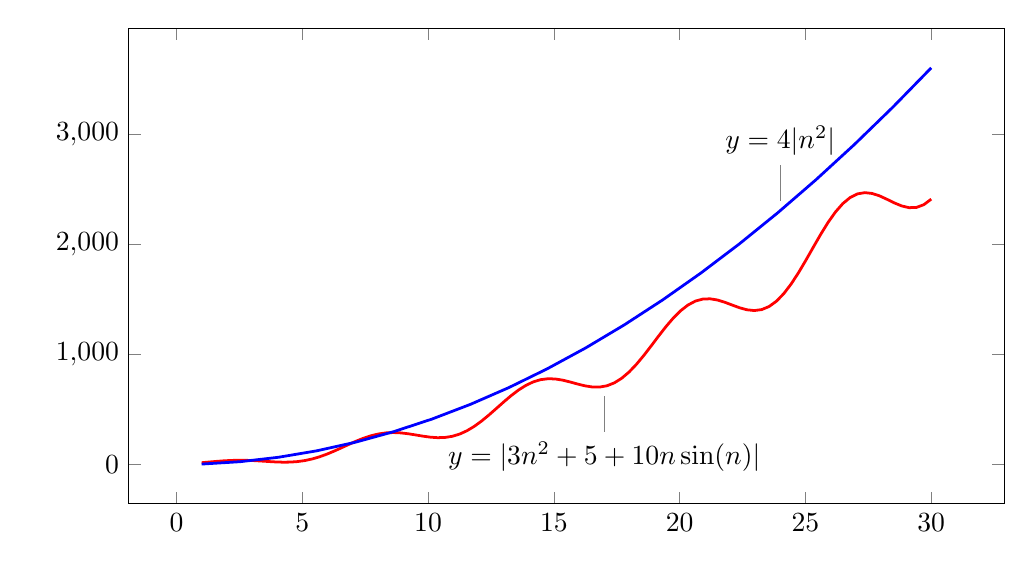
\begin{tikzpicture}[line width=1]
\begin{axis}[width=5in, height=3in,
             scatter/classes={a={mark=*,draw=black}},
             xlabel={\mbox{}},
             xlabel style={name=xlabel}, 
             ylabel={\mbox{}}, 
             legend style={
                at={(xlabel.south)},
                yshift=-1ex,
                anchor=north,
                legend cell align=left,
                },
        ]
]
\addplot[draw=red, line width=1] coordinates {(1.0,16.4147)
(1.2929,22.4484)
(1.5859,28.4016)
(1.8788,33.4933)
(2.1717,37.0617)
(2.4646,38.6624)
(2.7576,38.1439)
(3.0505,35.6915)
(3.3434,31.8329)
(3.6364,27.4029)
(3.9293,23.4698)
(4.2222,21.2307)
(4.5152,21.8837)
(4.8081,26.4921)
(5.101,35.8545)
(5.3939,50.3946)
(5.6869,70.0841)
(5.9798,94.409)
(6.2727,122.3853)
(6.5657,152.624)
(6.8586,183.443)
(7.1515,213.0165)
(7.4444,239.5475)
(7.7374,261.4491)
(8.0303,277.5153)
(8.3232,287.0641)
(8.6162,290.0382)
(8.9091,287.0493)
(9.202,279.3606)
(9.4949,268.8049)
(9.7879,257.6437)
(10.0808,248.3776)
(10.3737,243.5245)
(10.6667,245.3845)
(10.9596,255.8132)
(11.2525,276.027)
(11.5455,306.4575)
(11.8384,346.6732)
(12.1313,395.3773)
(12.4242,450.4864)
(12.7172,509.2844)
(13.0101,568.6421)
(13.303,625.2839)
(13.596,676.0796)
(13.8889,718.3338)
(14.1818,750.0487)
(14.4747,770.1327)
(14.7677,778.5354)
(15.0606,776.2931)
(15.3535,765.4782)
(15.6465,749.0519)
(15.9394,730.6326)
(16.2323,714.1964)
(16.5253,703.7343)
(16.8182,702.8971)
(17.1111,714.6583)
(17.404,741.0255)
(17.697,782.8302)
(17.9899,839.6146)
(18.2828,909.6296)
(18.5758,989.9493)
(18.8687,1076.6916)
(19.1616,1165.3326)
(19.4545,1251.0864)
(19.7475,1329.3198)
(20.0404,1395.9654)
(20.3333,1447.8973)
(20.6263,1483.2335)
(20.9192,1501.5372)
(21.2121,1503.896)
(21.5051,1492.8688)
(21.798,1472.3013)
(22.0909,1447.0233)
(22.3838,1422.4513)
(22.6768,1404.1289)
(22.9697,1397.2441)
(23.2626,1406.1662)
(23.5556,1434.0418)
(23.8485,1482.4895)
(24.1414,1551.4195)
(24.4343,1639.0007)
(24.7273,1741.7775)
(25.0202,1854.9334)
(25.3131,1972.679)
(25.6061,2088.7345)
(25.899,2196.8663)
(26.1919,2291.4312)
(26.4848,2367.8821)
(26.7778,2423.1883)
(27.0707,2456.1332)
(27.3636,2467.4598)
(27.6566,2459.8485)
(27.9495,2437.7253)
(28.2424,2406.9141)
(28.5354,2374.1592)
(28.8283,2346.5586)
(29.1212,2330.9541)
(29.4141,2333.3321)
(29.7071,2358.2861)
(30.0,2408.5905)};\node[pin=below:{$y=|3n^2 + 5 + 10n \sin(n)|$}] at (axis cs:17,708.5624263804754) {};\addplot[draw=blue, line width=1] coordinates {(1.0,4.0)
(2.5263,25.5291)
(4.0526,65.6953)
(5.5789,124.4986)
(7.1053,201.9391)
(8.6316,298.0166)
(10.1579,412.7313)
(11.6842,546.0831)
(13.2105,698.072)
(14.7368,868.6981)
(16.2632,1057.9612)
(17.7895,1265.8615)
(19.3158,1492.3989)
(20.8421,1737.5734)
(22.3684,2001.385)
(23.8947,2283.8338)
(25.4211,2584.9197)
(26.9474,2904.6427)
(28.4737,3243.0028)
(30.0,3600.0)};\node[pin=above:{$y=4|n^2|$}] at (axis cs:24.0,2304.0) {};
\end{axis}\end{tikzpicture}\end{center}

we see that, for $n \geq N$, we have:
\[
|3n^2 + 5 + 10n \sin(n)| \leq C |n^2|
\]
i.e.,
\[
|f(n)| \leq C|g(n)|
\]
Hence $f(n) = O(g(n)$.
\qed

Remember that technically speaking you cannot prove a mathematical
fact like $f(n) = O(g(n))$ using graphs
because a graph cannot possibly show you that a multiple of $|g(n)|$
beats $|f(n)|$ for \textit{all} sufficiently large $n$.
A graph can only show you the graphs up to some \textit{finite} $n$.
How would you know that the graph 
of $|f(n)|$ won't suddenly shoot up and overtake $4|g(n)|$ at 
$n = 1000000000000$?
Later, I'll show you how to prove big-O statements without a shadow of doubt.

Now, let me give you another example.
Suppose I change my $f(n)$ to \textit{this}:
\[
f(n) = -3n^2 + 5 - 10 n \sin (n)
\]
then when I plot
$|-3n^2 + 5 - 10 n \sin (n)|$ 
and $4|n^2|$ for $0 \leq n \leq 5$,
I get
%-*-latex-*-

\begin{center}
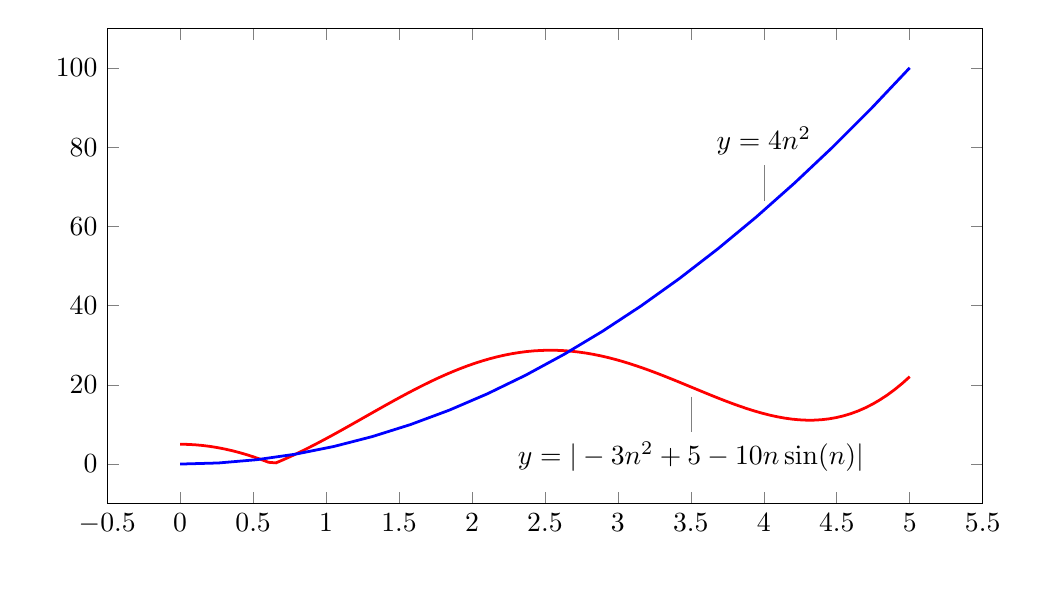
\begin{tikzpicture}[line width=1]
\begin{axis}[width=5in, height=3in,
             scatter/classes={a={mark=*,draw=black}},
             xlabel={\mbox{}},
             xlabel style={name=xlabel}, 
             ylabel={\mbox{}}, 
             legend style={
                at={(xlabel.south)},
                yshift=-1ex,
                anchor=north,
                legend cell align=left,
                },
        ]
]
\addplot[draw=red, line width=1] coordinates {(0.0,5.0)
(0.0505,4.9669)
(0.101,4.8675)
(0.1515,4.7024)
(0.202,4.4722)
(0.2525,4.1778)
(0.303,3.8202)
(0.3535,3.401)
(0.404,2.9218)
(0.4545,2.3845)
(0.5051,1.7911)
(0.5556,1.144)
(0.6061,0.4457)
(0.6566,0.3009)
(0.7071,1.093)
(0.7576,1.9275)
(0.8081,2.8011)
(0.8586,3.7103)
(0.9091,4.6516)
(0.9596,5.6212)
(1.0101,6.6153)
(1.0606,7.6301)
(1.1111,8.6614)
(1.1616,9.7053)
(1.2121,10.7576)
(1.2626,11.8141)
(1.3131,12.8708)
(1.3636,13.9233)
(1.4141,14.9676)
(1.4646,15.9996)
(1.5152,17.0151)
(1.5657,18.0102)
(1.6162,18.9809)
(1.6667,19.9235)
(1.7172,20.8341)
(1.7677,21.7093)
(1.8182,22.5456)
(1.8687,23.3398)
(1.9192,24.0888)
(1.9697,24.7897)
(2.0202,25.4397)
(2.0707,26.0365)
(2.1212,26.5779)
(2.1717,27.0617)
(2.2222,27.4864)
(2.2727,27.8503)
(2.3232,28.1524)
(2.3737,28.3917)
(2.4242,28.5676)
(2.4747,28.6797)
(2.5253,28.728)
(2.5758,28.7128)
(2.6263,28.6346)
(2.6768,28.4943)
(2.7273,28.2932)
(2.7778,28.0326)
(2.8283,27.7146)
(2.8788,27.3411)
(2.9293,26.9145)
(2.9798,26.4377)
(3.0303,25.9137)
(3.0808,25.3456)
(3.1313,24.7372)
(3.1818,24.0923)
(3.2323,23.4151)
(3.2828,22.7098)
(3.3333,21.9811)
(3.3838,21.2338)
(3.4343,20.4731)
(3.4848,19.7041)
(3.5354,18.9323)
(3.5859,18.1633)
(3.6364,17.4029)
(3.6869,16.6569)
(3.7374,15.9314)
(3.7879,15.2325)
(3.8384,14.5664)
(3.8889,13.9392)
(3.9394,13.3574)
(3.9899,12.8272)
(4.0404,12.3549)
(4.0909,11.9468)
(4.1414,11.6091)
(4.1919,11.3481)
(4.2424,11.1697)
(4.2929,11.08)
(4.3434,11.0848)
(4.3939,11.1899)
(4.4444,11.4007)
(4.4949,11.7226)
(4.5455,12.1608)
(4.596,12.7201)
(4.6465,13.4052)
(4.697,14.2205)
(4.7475,15.17)
(4.798,16.2577)
(4.8485,17.4869)
(4.899,18.8608)
(4.9495,20.3823)
(5.0,22.0538)
(5.0,22.0538)};\node[pin=below:{$y=|-3n^2+5-10n \sin(n)|$}] at (axis cs:3.5,19.472587030863306) {};\addplot[draw=blue, line width=1] coordinates {(0.0,0.0)
(0.2632,0.277)
(0.5263,1.108)
(0.7895,2.4931)
(1.0526,4.4321)
(1.3158,6.9252)
(1.5789,9.9723)
(1.8421,13.5734)
(2.1053,17.7285)
(2.3684,22.4377)
(2.6316,27.7008)
(2.8947,33.518)
(3.1579,39.8892)
(3.4211,46.8144)
(3.6842,54.2936)
(3.9474,62.3269)
(4.2105,70.9141)
(4.4737,80.0554)
(4.7368,89.7507)
(5.0,100.0)};\node[pin=above:{$y=4 n^2$}] at (axis cs:4.0,64.0) {};
\end{axis}\end{tikzpicture}\end{center}

and then for $0 \leq n \leq 100$:
%-*-latex-*-

\begin{center}
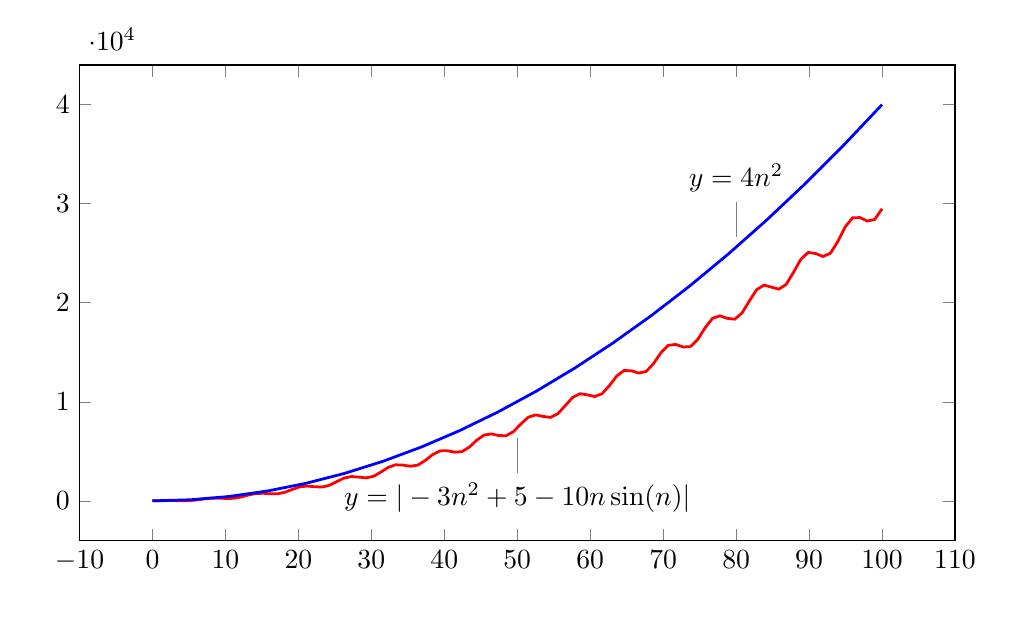
\begin{tikzpicture}[line width=1]
\begin{axis}[width=5in, height=3in,
             scatter/classes={a={mark=*,draw=black}},
             xlabel={\mbox{}},
             xlabel style={name=xlabel}, 
             ylabel={\mbox{}}, 
             legend style={
                at={(xlabel.south)},
                yshift=-1ex,
                anchor=north,
                legend cell align=left,
                },
        ]
]
\addplot[draw=red, line width=1] coordinates {(0.0,5.0)
(1.0101,6.6153)
(2.0202,25.4397)
(3.0303,25.9137)
(4.0404,12.3549)
(5.0505,23.8773)
(6.0606,91.8143)
(7.0707,195.0882)
(8.0808,269.6366)
(9.0909,272.7249)
(10.101,237.8732)
(11.1111,255.0)
(12.1212,383.5773)
(13.1313,582.5949)
(14.1414,736.3516)
(15.1515,763.7315)
(16.1616,707.7649)
(17.1717,708.8693)
(18.1818,874.1517)
(19.1919,1164.4193)
(20.202,1416.5891)
(21.2121,1493.896)
(22.2222,1425.5875)
(23.2323,1394.4064)
(24.2424,1569.656)
(25.2525,1938.2463)
(26.2626,2301.6861)
(27.2727,2456.1335)
(28.2828,2392.3527)
(29.2929,2319.8353)
(30.303,2478.008)
(31.3131,2904.4048)
(32.3232,3384.0318)
(33.3333,3641.8432)
(34.3434,3606.3782)
(35.3535,3491.9899)
(36.3636,3608.3278)
(37.3737,4065.9185)
(38.3838,4657.72)
(39.3939,5041.5605)
(40.404,5063.3358)
(41.4141,4915.7123)
(42.4242,4970.241)
(43.4343,5428.359)
(44.4444,6119.0909)
(45.4545,6645.6871)
(46.4646,6756.4949)
(47.4747,6593.3826)
(48.4848,6573.1284)
(49.4949,6999.509)
(50.5051,7767.1203)
(51.5152,8445.2496)
(52.5253,8677.1483)
(53.5354,8524.6161)
(54.5455,8425.3713)
(55.5556,8788.8539)
(56.5657,9603.6299)
(57.5758,10432.6353)
(58.5859,10815.1947)
(59.596,10706.1514)
(60.6061,10533.6472)
(61.6162,10806.9348)
(62.6263,11633.2978)
(63.6364,12602.2548)
(64.6465,13159.841)
(65.6566,13131.942)
(66.6667,12902.3213)
(67.6768,13064.6013)
(68.6869,13863.4655)
(69.697,14951.0841)
(70.7071,15700.3808)
(71.7172,15793.4493)
(72.7273,15532.9807)
(73.7374,15572.215)
(74.7475,16303.7479)
(75.7576,17479.0458)
(76.7677,18426.9974)
(77.7778,18680.1241)
(78.7879,18424.1447)
(79.798,18338.8533)
(80.8081,18965.4674)
(81.8182,20189.2011)
(82.8283,21331.5386)
(83.8384,21780.0485)
(84.8485,21571.1764)
(85.8586,21371.5687)
(86.8687,21860.9452)
(87.8788,23087.7309)
(88.8889,24408.2113)
(89.899,25080.7016)
(90.9091,24966.4088)
(91.9192,24674.7531)
(92.9293,25002.6904)
(93.9394,26183.7035)
(94.9495,27654.146)
(95.9596,28569.8024)
(96.9697,28599.4829)
(97.9798,28249.6545)
(98.9899,28402.5388)
(100.0,29488.6344)};\node[pin=below:{$y=|-3n^2+5-10n \sin(n)|$}] at (axis cs:50,7363.812573148036) {};\addplot[draw=blue, line width=1] coordinates {(0.0,0.0)
(5.2632,110.8033)
(10.5263,443.2133)
(15.7895,997.2299)
(21.0526,1772.8532)
(26.3158,2770.0831)
(31.5789,3988.9197)
(36.8421,5429.3629)
(42.1053,7091.4127)
(47.3684,8975.0693)
(52.6316,11080.3324)
(57.8947,13407.2022)
(63.1579,15955.6787)
(68.4211,18725.7618)
(73.6842,21717.4515)
(78.9474,24930.7479)
(84.2105,28365.651)
(89.4737,32022.1607)
(94.7368,35900.277)
(100.0,40000.0)};\node[pin=above:{$y=4 n^2$}] at (axis cs:80.0,25600.0) {};
\end{axis}\end{tikzpicture}\end{center}

In this case $n^2$ still works, i.e., 
$-3n^2 + 5 - 10 n \sin (n) = O(n^2)$.
Also, it seems that $4n^2$ breaks away from 
$|-3n^2+5-10n \sin(n)|$ around $n = 20$.
So let's plot the graphs for $0 \leq n \leq 20$:
%-*-latex-*-

\begin{center}
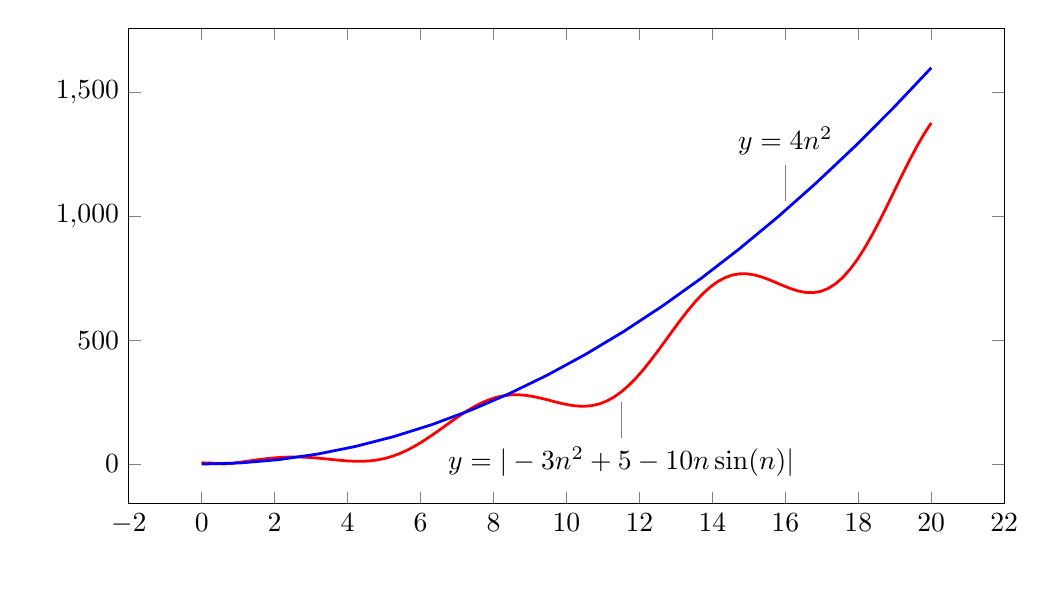
\begin{tikzpicture}[line width=1]
\begin{axis}[width=5in, height=3in,
             scatter/classes={a={mark=*,draw=black}},
             xlabel={\mbox{}},
             xlabel style={name=xlabel}, 
             ylabel={\mbox{}}, 
             legend style={
                at={(xlabel.south)},
                yshift=-1ex,
                anchor=north,
                legend cell align=left,
                },
        ]
]
\addplot[draw=red, line width=1] coordinates {(0.0,5.0)
(0.202,4.4722)
(0.404,2.9218)
(0.6061,0.4457)
(0.8081,2.8011)
(1.0101,6.6153)
(1.2121,10.7576)
(1.4141,14.9676)
(1.6162,18.9809)
(1.8182,22.5456)
(2.0202,25.4397)
(2.2222,27.4864)
(2.4242,28.5676)
(2.6263,28.6346)
(2.8283,27.7146)
(3.0303,25.9137)
(3.2323,23.4151)
(3.4343,20.4731)
(3.6364,17.4029)
(3.8384,14.5664)
(4.0404,12.3549)
(4.2424,11.1697)
(4.4444,11.4007)
(4.6465,13.4052)
(4.8485,17.4869)
(5.0505,23.8773)
(5.2525,32.7194)
(5.4545,44.0555)
(5.6566,57.8195)
(5.8586,73.8343)
(6.0606,91.8143)
(6.2626,111.374)
(6.4646,132.0415)
(6.6667,153.2767)
(6.8687,174.4941)
(7.0707,195.0882)
(7.2727,214.4613)
(7.4747,232.0521)
(7.6768,247.3637)
(7.8788,259.9895)
(8.0808,269.6366)
(8.2828,276.1436)
(8.4848,279.4945)
(8.6869,279.8253)
(8.8889,277.4242)
(9.0909,272.7249)
(9.2929,266.2927)
(9.4949,258.8049)
(9.697,251.024)
(9.899,243.7675)
(10.101,237.8732)
(10.303,234.1627)
(10.5051,233.4047)
(10.7071,236.2785)
(10.9091,243.3416)
(11.1111,255.0)
(11.3131,271.486)
(11.5152,292.8413)
(11.7172,318.9095)
(11.9192,349.3361)
(12.1212,383.5773)
(12.3232,420.918)
(12.5253,460.4972)
(12.7273,501.3406)
(12.9293,542.3998)
(13.1313,582.5949)
(13.3333,620.8602)
(13.5354,656.1907)
(13.7374,687.687)
(13.9394,714.5968)
(14.1414,736.3516)
(14.3434,752.5962)
(14.5455,763.2092)
(14.7475,768.3154)
(14.9495,768.2864)
(15.1515,763.7315)
(15.3535,755.4782)
(15.5556,744.5421)
(15.7576,732.0891)
(15.9596,719.389)
(16.1616,707.7649)
(16.3636,698.5379)
(16.5657,692.971)
(16.7677,692.2147)
(16.9697,697.2553)
(17.1717,708.8693)
(17.3737,727.5859)
(17.5758,753.659)
(17.7778,787.0499)
(17.9798,827.4227)
(18.1818,874.1517)
(18.3838,926.3413)
(18.5859,982.858)
(18.7879,1042.3727)
(18.9899,1103.4124)
(19.1919,1164.4193)
(19.3939,1223.8141)
(19.596,1280.062)
(19.798,1331.7381)
(20.0,1377.5891)
(20.0,1377.5891)};\node[pin=below:{$y=|-3n^2+5-10n \sin(n)|$}] at (axis cs:11.5,291.07299991083073) {};\addplot[draw=blue, line width=1] coordinates {(0.0,0.0)
(1.0526,4.4321)
(2.1053,17.7285)
(3.1579,39.8892)
(4.2105,70.9141)
(5.2632,110.8033)
(6.3158,159.5568)
(7.3684,217.1745)
(8.4211,283.6565)
(9.4737,359.0028)
(10.5263,443.2133)
(11.5789,536.2881)
(12.6316,638.2271)
(13.6842,749.0305)
(14.7368,868.6981)
(15.7895,997.2299)
(16.8421,1134.626)
(17.8947,1280.8864)
(18.9474,1436.0111)
(20.0,1600.0)};\node[pin=above:{$y=4 n^2$}] at (axis cs:16.0,1024.0) {};
\end{axis}\end{tikzpicture}\end{center}

Clearly for $n \geq 10$, $4|g(n)|$ beats $|f(n)|$.
So I'm going to pick $N = 10$.

Now I'm ready to present this ...

\newpage

\begin{eg}
Let $f(n) = -3n^2+5-10n \sin(n)$ and $g(n) = n^2$.
Show graphically that 
\[
f(n) = O(g(n))
\]
\end{eg}

\textit{Solution.}
From the following graphs:
%-*-latex-*-

\begin{center}
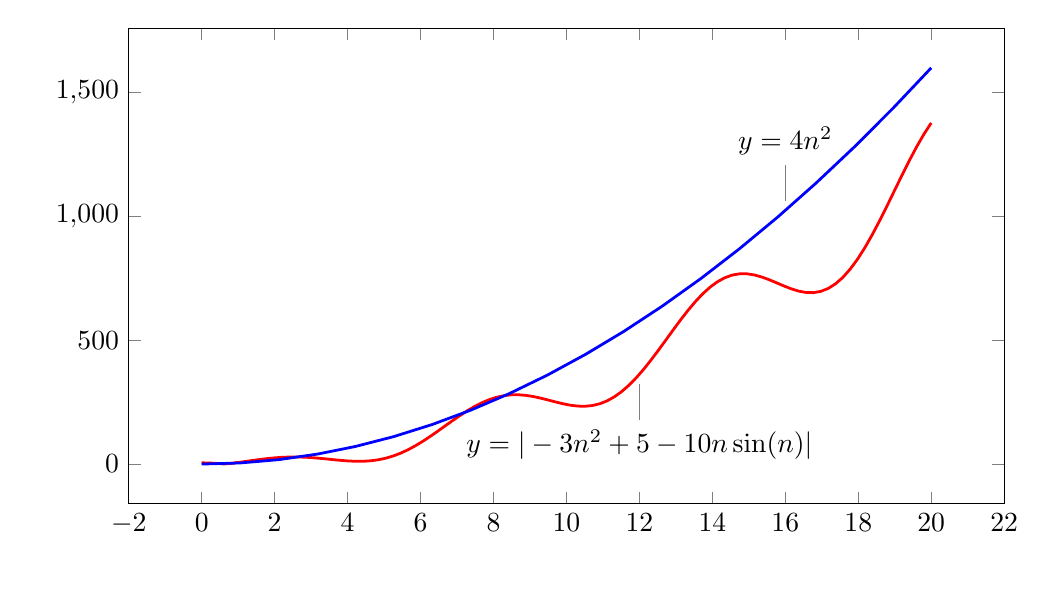
\begin{tikzpicture}[line width=1]
\begin{axis}[width=5in, height=3in,
             scatter/classes={a={mark=*,draw=black}},
             xlabel={\mbox{}},
             xlabel style={name=xlabel}, 
             ylabel={\mbox{}}, 
             legend style={
                at={(xlabel.south)},
                yshift=-1ex,
                anchor=north,
                legend cell align=left,
                },
        ]
]
\addplot[draw=red, line width=1] coordinates {(0.0,5.0)
(0.202,4.4722)
(0.404,2.9218)
(0.6061,0.4457)
(0.8081,2.8011)
(1.0101,6.6153)
(1.2121,10.7576)
(1.4141,14.9676)
(1.6162,18.9809)
(1.8182,22.5456)
(2.0202,25.4397)
(2.2222,27.4864)
(2.4242,28.5676)
(2.6263,28.6346)
(2.8283,27.7146)
(3.0303,25.9137)
(3.2323,23.4151)
(3.4343,20.4731)
(3.6364,17.4029)
(3.8384,14.5664)
(4.0404,12.3549)
(4.2424,11.1697)
(4.4444,11.4007)
(4.6465,13.4052)
(4.8485,17.4869)
(5.0505,23.8773)
(5.2525,32.7194)
(5.4545,44.0555)
(5.6566,57.8195)
(5.8586,73.8343)
(6.0606,91.8143)
(6.2626,111.374)
(6.4646,132.0415)
(6.6667,153.2767)
(6.8687,174.4941)
(7.0707,195.0882)
(7.2727,214.4613)
(7.4747,232.0521)
(7.6768,247.3637)
(7.8788,259.9895)
(8.0808,269.6366)
(8.2828,276.1436)
(8.4848,279.4945)
(8.6869,279.8253)
(8.8889,277.4242)
(9.0909,272.7249)
(9.2929,266.2927)
(9.4949,258.8049)
(9.697,251.024)
(9.899,243.7675)
(10.101,237.8732)
(10.303,234.1627)
(10.5051,233.4047)
(10.7071,236.2785)
(10.9091,243.3416)
(11.1111,255.0)
(11.3131,271.486)
(11.5152,292.8413)
(11.7172,318.9095)
(11.9192,349.3361)
(12.1212,383.5773)
(12.3232,420.918)
(12.5253,460.4972)
(12.7273,501.3406)
(12.9293,542.3998)
(13.1313,582.5949)
(13.3333,620.8602)
(13.5354,656.1907)
(13.7374,687.687)
(13.9394,714.5968)
(14.1414,736.3516)
(14.3434,752.5962)
(14.5455,763.2092)
(14.7475,768.3154)
(14.9495,768.2864)
(15.1515,763.7315)
(15.3535,755.4782)
(15.5556,744.5421)
(15.7576,732.0891)
(15.9596,719.389)
(16.1616,707.7649)
(16.3636,698.5379)
(16.5657,692.971)
(16.7677,692.2147)
(16.9697,697.2553)
(17.1717,708.8693)
(17.3737,727.5859)
(17.5758,753.659)
(17.7778,787.0499)
(17.9798,827.4227)
(18.1818,874.1517)
(18.3838,926.3413)
(18.5859,982.858)
(18.7879,1042.3727)
(18.9899,1103.4124)
(19.1919,1164.4193)
(19.3939,1223.8141)
(19.596,1280.062)
(19.798,1331.7381)
(20.0,1377.5891)
(20.0,1377.5891)};\node[pin=below:{$y=|-3n^2+5-10n \sin(n)|$}] at (axis cs:12,362.6112498399478) {};\addplot[draw=blue, line width=1] coordinates {(0.0,0.0)
(1.0526,4.4321)
(2.1053,17.7285)
(3.1579,39.8892)
(4.2105,70.9141)
(5.2632,110.8033)
(6.3158,159.5568)
(7.3684,217.1745)
(8.4211,283.6565)
(9.4737,359.0028)
(10.5263,443.2133)
(11.5789,536.2881)
(12.6316,638.2271)
(13.6842,749.0305)
(14.7368,868.6981)
(15.7895,997.2299)
(16.8421,1134.626)
(17.8947,1280.8864)
(18.9474,1436.0111)
(20.0,1600.0)};\node[pin=above:{$y=4 n^2$}] at (axis cs:16.0,1024.0) {};
\end{axis}\end{tikzpicture}\end{center}

%-*-latex-*-

\begin{center}
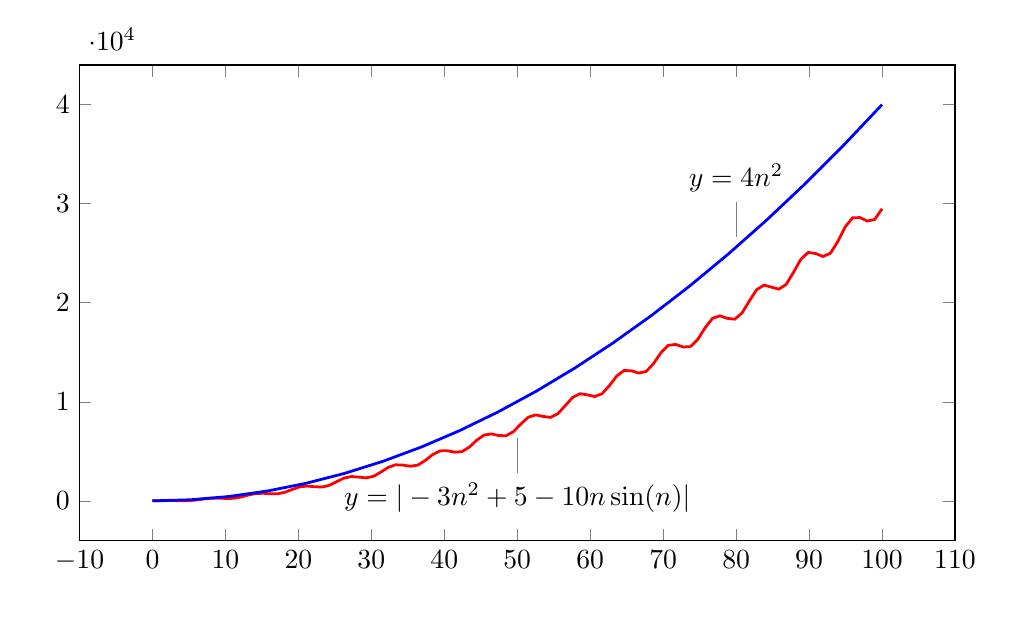
\begin{tikzpicture}[line width=1]
\begin{axis}[width=5in, height=3in,
             scatter/classes={a={mark=*,draw=black}},
             xlabel={\mbox{}},
             xlabel style={name=xlabel}, 
             ylabel={\mbox{}}, 
             legend style={
                at={(xlabel.south)},
                yshift=-1ex,
                anchor=north,
                legend cell align=left,
                },
        ]
]
\addplot[draw=red, line width=1] coordinates {(0.0,5.0)
(1.0101,6.6153)
(2.0202,25.4397)
(3.0303,25.9137)
(4.0404,12.3549)
(5.0505,23.8773)
(6.0606,91.8143)
(7.0707,195.0882)
(8.0808,269.6366)
(9.0909,272.7249)
(10.101,237.8732)
(11.1111,255.0)
(12.1212,383.5773)
(13.1313,582.5949)
(14.1414,736.3516)
(15.1515,763.7315)
(16.1616,707.7649)
(17.1717,708.8693)
(18.1818,874.1517)
(19.1919,1164.4193)
(20.202,1416.5891)
(21.2121,1493.896)
(22.2222,1425.5875)
(23.2323,1394.4064)
(24.2424,1569.656)
(25.2525,1938.2463)
(26.2626,2301.6861)
(27.2727,2456.1335)
(28.2828,2392.3527)
(29.2929,2319.8353)
(30.303,2478.008)
(31.3131,2904.4048)
(32.3232,3384.0318)
(33.3333,3641.8432)
(34.3434,3606.3782)
(35.3535,3491.9899)
(36.3636,3608.3278)
(37.3737,4065.9185)
(38.3838,4657.72)
(39.3939,5041.5605)
(40.404,5063.3358)
(41.4141,4915.7123)
(42.4242,4970.241)
(43.4343,5428.359)
(44.4444,6119.0909)
(45.4545,6645.6871)
(46.4646,6756.4949)
(47.4747,6593.3826)
(48.4848,6573.1284)
(49.4949,6999.509)
(50.5051,7767.1203)
(51.5152,8445.2496)
(52.5253,8677.1483)
(53.5354,8524.6161)
(54.5455,8425.3713)
(55.5556,8788.8539)
(56.5657,9603.6299)
(57.5758,10432.6353)
(58.5859,10815.1947)
(59.596,10706.1514)
(60.6061,10533.6472)
(61.6162,10806.9348)
(62.6263,11633.2978)
(63.6364,12602.2548)
(64.6465,13159.841)
(65.6566,13131.942)
(66.6667,12902.3213)
(67.6768,13064.6013)
(68.6869,13863.4655)
(69.697,14951.0841)
(70.7071,15700.3808)
(71.7172,15793.4493)
(72.7273,15532.9807)
(73.7374,15572.215)
(74.7475,16303.7479)
(75.7576,17479.0458)
(76.7677,18426.9974)
(77.7778,18680.1241)
(78.7879,18424.1447)
(79.798,18338.8533)
(80.8081,18965.4674)
(81.8182,20189.2011)
(82.8283,21331.5386)
(83.8384,21780.0485)
(84.8485,21571.1764)
(85.8586,21371.5687)
(86.8687,21860.9452)
(87.8788,23087.7309)
(88.8889,24408.2113)
(89.899,25080.7016)
(90.9091,24966.4088)
(91.9192,24674.7531)
(92.9293,25002.6904)
(93.9394,26183.7035)
(94.9495,27654.146)
(95.9596,28569.8024)
(96.9697,28599.4829)
(97.9798,28249.6545)
(98.9899,28402.5388)
(100.0,29488.6344)};\node[pin=below:{$y=|-3n^2+5-10n \sin(n)|$}] at (axis cs:50,7363.812573148036) {};\addplot[draw=blue, line width=1] coordinates {(0.0,0.0)
(5.2632,110.8033)
(10.5263,443.2133)
(15.7895,997.2299)
(21.0526,1772.8532)
(26.3158,2770.0831)
(31.5789,3988.9197)
(36.8421,5429.3629)
(42.1053,7091.4127)
(47.3684,8975.0693)
(52.6316,11080.3324)
(57.8947,13407.2022)
(63.1579,15955.6787)
(68.4211,18725.7618)
(73.6842,21717.4515)
(78.9474,24930.7479)
(84.2105,28365.651)
(89.4737,32022.1607)
(94.7368,35900.277)
(100.0,40000.0)};\node[pin=above:{$y=4 n^2$}] at (axis cs:80.0,25600.0) {};
\end{axis}\end{tikzpicture}\end{center}

we see that if we choose $C = 4$ and $N  = 20$, then for $n \geq N$,
we have
\[
|-3n^2+5-10n \sin(n)| \leq 4|n^2|
\]
i.e.,
\[
|f(n)| \leq C|g(n)|
\]
Hence $f(n) = O(g(n))$.
\qed

\newpage

It's not surprising that if 
\[
3n^2 + 5 + 10 n \sin (n) = O(n^2)
\]
then it is also true that 
\[
3n^2 + 5 + 10 n \sin (n) = O(n^3)
\]
since $n^3$ grows faster than $n^2$.
So there are many possible functions to \lq\lq control''
$3n^2 + 5 + 10n \sin(n)$ from above.
Also, if
\[
|3n^2 + 5 + 10 n \sin (n)| \leq C|n^2|
\]
then of course if you replace $C$ by a large value, say $C + 1423$,
then of course
\[
|3n^2 + 5 + 10 n \sin (n)| \leq (C + 1423)|n^2|
\]
is still true for $n \geq N$.
Furthermore, this is also true if you replace $N$ by a larger value
such as $N + 15313$.
Therefore the choice of $C$ and $N$ is not unique.


Here's another example.

Let
\[
f(n) = \frac{2n^5}{1 + n} \sin \frac{1000}{n} - 100
\]
Let's find some function $g(n)$ of the form $n^0, n^1, n^2, n^3$ or ...
such that $f(n) = O(g(n))$.
Let's have a few plots to get a feel for the function.

Here's the plot of $f(n)$ for $0 \leq n \leq 10$:
%-*-latex-*-

\begin{center}
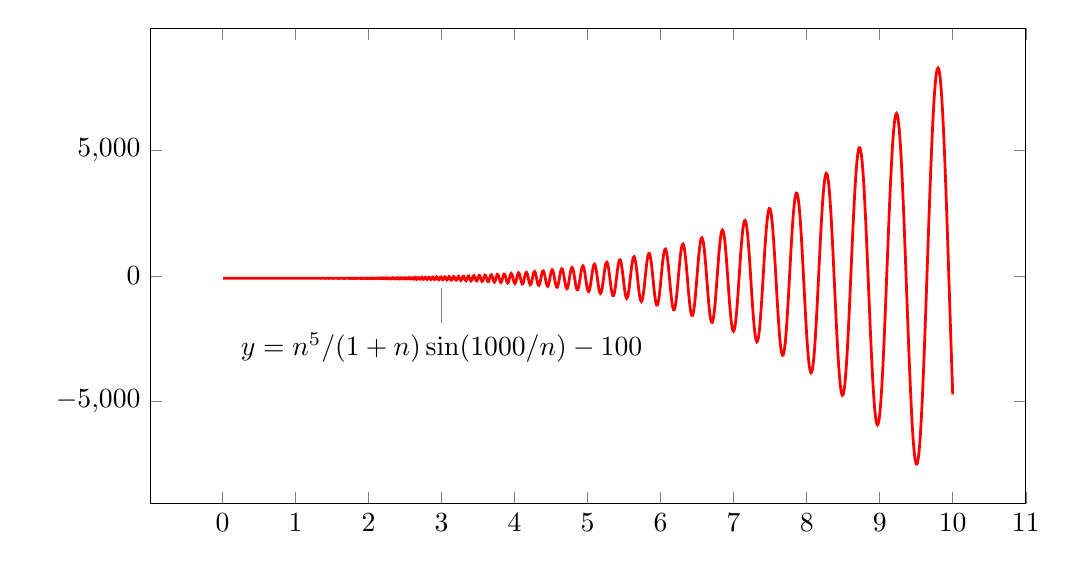
\begin{tikzpicture}[line width=1]
\begin{axis}[width=5in, height=3in,
             scatter/classes={a={mark=*,draw=black}},
             xlabel={\mbox{}},
             xlabel style={name=xlabel}, 
             ylabel={\mbox{}}, 
             legend style={
                at={(xlabel.south)},
                yshift=-1ex,
                anchor=north,
                legend cell align=left,
                },
        ]
]
\addplot[draw=red, line width=1] coordinates {(0.01,-100.0)
(0.02,-100.0)
(0.03,-100.0)
(0.04,-100.0)
(0.0501,-100.0)
(0.0601,-100.0)
(0.0701,-100.0)
(0.0801,-100.0)
(0.0901,-100.0)
(0.1001,-100.0)
(0.1101,-100.0)
(0.1201,-100.0)
(0.1301,-100.0)
(0.1401,-100.0)
(0.1502,-100.0)
(0.1602,-100.0001)
(0.1702,-99.9999)
(0.1802,-99.9999)
(0.1902,-100.0002)
(0.2002,-100.0)
(0.2102,-99.9998)
(0.2202,-100.0004)
(0.2302,-99.9995)
(0.2402,-99.9999)
(0.2503,-100.0001)
(0.2603,-100.0001)
(0.2703,-100.0008)
(0.2803,-100.0011)
(0.2903,-99.9984)
(0.3003,-100.0002)
(0.3103,-100.0014)
(0.3203,-100.0019)
(0.3303,-100.0028)
(0.3403,-100.0026)
(0.3504,-99.9961)
(0.3604,-100.0037)
(0.3704,-100.005)
(0.3804,-99.9969)
(0.3904,-100.0059)
(0.4004,-99.9995)
(0.4104,-100.0079)
(0.4204,-100.0035)
(0.4304,-100.0103)
(0.4404,-99.9909)
(0.4505,-99.9886)
(0.4605,-100.0111)
(0.4705,-99.9848)
(0.4805,-99.9827)
(0.4905,-99.9978)
(0.5005,-100.0011)
(0.5105,-100.0229)
(0.5205,-100.0251)
(0.5305,-100.0014)
(0.5405,-99.9884)
(0.5506,-99.9837)
(0.5606,-100.0169)
(0.5706,-100.0142)
(0.5806,-99.9695)
(0.5906,-99.9956)
(0.6006,-100.0022)
(0.6106,-100.0424)
(0.6206,-99.9807)
(0.6306,-99.9565)
(0.6406,-99.9723)
(0.6507,-100.0447)
(0.6607,-100.0435)
(0.6707,-99.924)
(0.6807,-100.0793)
(0.6907,-99.9597)
(0.7007,-99.9247)
(0.7107,-100.0404)
(0.7207,-100.0999)
(0.7307,-100.1139)
(0.7407,-100.0991)
(0.7508,-100.0048)
(0.7608,-99.861)
(0.7708,-99.9885)
(0.7808,-100.1372)
(0.7908,-99.8277)
(0.8008,-100.1828)
(0.8108,-99.8129)
(0.8208,-100.1231)
(0.8308,-100.0811)
(0.8408,-99.7759)
(0.8509,-99.92)
(0.8609,-100.1753)
(0.8709,-100.2677)
(0.8809,-100.2529)
(0.8909,-100.2367)
(0.9009,-100.2657)
(0.9109,-100.3226)
(0.9209,-100.3106)
(0.9309,-100.083)
(0.9409,-99.7005)
(0.951,-99.6993)
(0.961,-100.2872)
(0.971,-100.2272)
(0.981,-99.5422)
(0.991,-100.2866)
(1.001,-100.0133)
(1.011,-99.7515)
(1.021,-100.3803)
(1.031,-99.5693)
(1.041,-100.4085)
(1.0511,-99.7145)
(1.0611,-100.0163)
(1.0711,-100.3797)
(1.0811,-99.3044)
(1.0911,-100.5463)
(1.1011,-100.1992)
(1.1111,-99.1996)
(1.1211,-100.205)
(1.1311,-100.8332)
(1.1411,-99.8306)
(1.1512,-99.0613)
(1.1612,-99.6102)
(1.1712,-100.6279)
(1.1812,-101.0529)
(1.1912,-100.6972)
(1.2012,-99.9749)
(1.2112,-99.316)
(1.2212,-98.9084)
(1.2312,-98.7374)
(1.2412,-98.7051)
(1.2513,-98.7135)
(1.2613,-98.6972)
(1.2713,-98.6291)
(1.2813,-98.5218)
(1.2913,-98.4333)
(1.3013,-98.4725)
(1.3113,-98.7831)
(1.3213,-99.4779)
(1.3313,-100.5081)
(1.3413,-101.5244)
(1.3514,-101.8936)
(1.3614,-101.075)
(1.3714,-99.3033)
(1.3814,-97.9406)
(1.3914,-98.5626)
(1.4014,-100.9381)
(1.4114,-102.315)
(1.4214,-100.4658)
(1.4314,-97.7263)
(1.4414,-98.6852)
(1.4515,-102.1477)
(1.4615,-101.5752)
(1.4715,-97.6395)
(1.4815,-98.7688)
(1.4915,-102.8627)
(1.5015,-100.0538)
(1.5115,-96.9846)
(1.5215,-101.9416)
(1.5315,-101.6252)
(1.5415,-96.5773)
(1.5516,-101.6573)
(1.5616,-101.7388)
(1.5716,-96.3051)
(1.5816,-102.7984)
(1.5916,-100.0656)
(1.6016,-97.0887)
(1.6116,-104.1607)
(1.6216,-96.6112)
(1.6316,-101.1842)
(1.6416,-101.4311)
(1.6517,-96.4487)
(1.6617,-104.6718)
(1.6717,-95.2906)
(1.6817,-103.8715)
(1.6917,-97.5104)
(1.7017,-100.8896)
(1.7117,-100.6794)
(1.7217,-97.9346)
(1.7317,-103.2022)
(1.7417,-95.9153)
(1.7518,-104.7427)
(1.7618,-94.7808)
(1.7718,-105.5553)
(1.7818,-94.2201)
(1.7918,-105.9045)
(1.8018,-94.0809)
(1.8118,-105.792)
(1.8218,-94.5292)
(1.8318,-104.8871)
(1.8418,-96.0333)
(1.8519,-102.6468)
(1.8619,-99.0985)
(1.8719,-98.7737)
(1.8819,-103.5905)
(1.8919,-94.0828)
(1.9019,-107.8044)
(1.9119,-91.2332)
(1.9219,-108.3379)
(1.9319,-93.7686)
(1.9419,-102.5287)
(1.952,-102.1706)
(1.962,-93.268)
(1.972,-109.6948)
(1.982,-90.2638)
(1.992,-106.3004)
(2.002,-99.8583)
(2.012,-93.4337)
(2.022,-110.8471)
(2.032,-89.7559)
(2.042,-104.3574)
(2.0521,-104.3135)
(2.0621,-88.9055)
(2.0721,-111.573)
(2.0821,-95.3475)
(2.0921,-94.1491)
(2.1021,-112.8617)
(2.1121,-89.2482)
(2.1221,-100.1721)
(2.1321,-111.165)
(2.1421,-86.2686)
(2.1522,-104.3922)
(2.1622,-109.4646)
(2.1722,-84.875)
(2.1822,-106.2788)
(2.1922,-109.388)
(2.2022,-83.9634)
(2.2122,-105.7045)
(2.2222,-111.4917)
(2.2322,-83.6447)
(2.2422,-102.1623)
(2.2523,-115.3265)
(2.2623,-85.449)
(2.2723,-95.1491)
(2.2823,-118.7818)
(2.2923,-91.8666)
(2.3023,-85.839)
(2.3123,-117.5281)
(2.3223,-104.1439)
(2.3323,-79.3426)
(2.3423,-106.9063)
(2.3524,-117.9793)
(2.3624,-84.1523)
(2.3724,-88.4371)
(2.3824,-121.3509)
(2.3924,-103.6763)
(2.4024,-76.4811)
(2.4124,-103.9897)
(2.4224,-123.2152)
(2.4324,-89.4886)
(2.4424,-78.4954)
(2.4525,-115.5909)
(2.4625,-119.3337)
(2.4725,-80.691)
(2.4825,-82.5854)
(2.4925,-121.8984)
(2.5025,-116.2298)
(2.5125,-76.4175)
(2.5225,-83.9191)
(2.5325,-124.476)
(2.5425,-117.1332)
(2.5526,-75.4692)
(2.5626,-80.5715)
(2.5726,-123.5181)
(2.5826,-122.8565)
(2.5926,-78.9562)
(2.6026,-72.9149)
(2.6126,-116.6155)
(2.6226,-131.4681)
(2.6326,-90.2189)
(2.6426,-65.0309)
(2.6527,-100.3591)
(2.6627,-136.1652)
(2.6727,-111.2488)
(2.6827,-66.5771)
(2.6927,-76.269)
(2.7027,-125.3258)
(2.7127,-134.6763)
(2.7227,-88.6249)
(2.7327,-59.2491)
(2.7427,-92.829)
(2.7528,-138.4801)
(2.7628,-126.6767)
(2.7728,-74.2894)
(2.7828,-58.7105)
(2.7928,-103.4479)
(2.8028,-144.4373)
(2.8128,-122.7875)
(2.8228,-68.2253)
(2.8328,-56.6493)
(2.8428,-104.7187)
(2.8529,-147.6561)
(2.8629,-127.4459)
(2.8729,-70.1016)
(2.8829,-50.5877)
(2.8929,-94.8274)
(2.9029,-146.8884)
(2.9129,-140.805)
(2.9229,-83.3933)
(2.9329,-45.056)
(2.9429,-72.9663)
(2.953,-134.2823)
(2.963,-156.2209)
(2.973,-112.3702)
(2.983,-52.9834)
(2.993,-46.2618)
(3.003,-100.5382)
(3.013,-155.5643)
(3.023,-150.2114)
(3.033,-89.593)
(3.043,-38.7764)
(3.0531,-52.357)
(3.0631,-116.7428)
(3.0731,-165.158)
(3.0831,-147.3267)
(3.0931,-80.6805)
(3.1031,-31.9667)
(3.1131,-50.034)
(3.1231,-117.8389)
(3.1331,-169.8365)
(3.1431,-155.726)
(3.1532,-88.1914)
(3.1632,-30.2144)
(3.1732,-35.861)
(3.1832,-100.6502)
(3.1932,-166.3266)
(3.2032,-173.8673)
(3.2132,-115.9348)
(3.2232,-42.7)
(3.2332,-17.5855)
(3.2432,-62.665)
(3.2533,-140.4329)
(3.2633,-185.9931)
(3.2733,-161.2194)
(3.2833,-85.6927)
(3.2933,-20.1203)
(3.3033,-17.1679)
(3.3133,-79.8156)
(3.3233,-159.6335)
(3.3333,-194.9436)
(3.3433,-158.2441)
(3.3534,-76.6251)
(3.3634,-10.7952)
(3.3734,-9.6847)
(3.3834,-74.739)
(3.3934,-159.4614)
(3.4034,-203.329)
(3.4134,-174.8611)
(3.4234,-93.3229)
(3.4334,-14.7371)
(3.4434,6.9867)
(3.4535,-43.415)
(3.4635,-132.8045)
(3.4735,-202.2344)
(3.4835,-205.9565)
(3.4935,-140.9551)
(3.5035,-48.3478)
(3.5135,13.2874)
(3.5235,4.9412)
(3.5335,-68.8218)
(3.5435,-163.2172)
(3.5536,-220.9944)
(3.5636,-207.0542)
(3.5736,-129.0734)
(3.5836,-32.4443)
(3.5936,26.6619)
(3.6036,13.8306)
(3.6136,-64.2283)
(3.6236,-163.9863)
(3.6336,-229.8827)
(3.6436,-225.1968)
(3.6537,-151.9038)
(3.6637,-49.1185)
(3.6737,28.3288)
(3.6837,39.1637)
(3.6937,-22.8438)
(3.7037,-126.0836)
(3.7137,-217.8269)
(3.7237,-251.3134)
(3.7337,-209.2176)
(3.7437,-111.9136)
(3.7538,-6.9539)
(3.7638,54.4841)
(3.7738,42.3722)
(3.7838,-38.071)
(3.7938,-149.2919)
(3.8038,-239.4049)
(3.8138,-266.4424)
(3.8238,-217.5042)
(3.8338,-114.2599)
(3.8438,-2.7648)
(3.8539,67.3644)
(3.8639,64.8811)
(3.8739,-9.6737)
(3.8839,-124.6003)
(3.8939,-230.9981)
(3.9039,-283.706)
(3.9139,-260.2091)
(3.9239,-169.7138)
(3.9339,-48.9672)
(3.9439,53.0556)
(3.954,95.06)
(3.964,59.8343)
(3.974,-39.239)
(3.984,-163.8028)
(3.994,-265.7136)
(4.004,-305.6579)
(4.014,-268.0019)
(4.024,-166.3913)
(4.034,-38.2997)
(4.044,69.1136)
(4.0541,116.3856)
(4.0641,85.9629)
(4.0741,-11.7625)
(4.0841,-142.4905)
(4.0941,-260.3889)
(4.1041,-324.2276)
(4.1141,-311.5746)
(4.1241,-226.2484)
(4.1341,-96.7038)
(4.1441,33.8274)
(4.1542,121.9046)
(4.1642,138.2051)
(4.1742,76.9314)
(4.1842,-42.5969)
(4.1942,-182.4395)
(4.2042,-298.3106)
(4.2142,-353.5915)
(4.2242,-330.6551)
(4.2342,-236.0829)
(4.2442,-98.3609)
(4.2543,41.0217)
(4.2643,140.194)
(4.2743,169.3743)
(4.2843,119.5117)
(4.2943,4.685)
(4.3043,-142.2508)
(4.3143,-279.3187)
(4.3243,-367.4679)
(4.3343,-381.547)
(4.3443,-317.1653)
(4.3544,-191.6625)
(4.3644,-39.0954)
(4.3744,99.2193)
(4.3844,185.9235)
(4.3944,197.5483)
(4.4044,130.5626)
(4.4144,2.0652)
(4.4244,-154.9025)
(4.4344,-300.0578)
(4.4444,-396.2519)
(4.4545,-418.8378)
(4.4645,-361.7112)
(4.4745,-238.6124)
(4.4845,-79.5078)
(4.4945,76.923)
(4.5045,192.7602)
(4.5145,239.9437)
(4.5245,206.8396)
(4.5345,100.7975)
(4.5445,-53.7886)
(4.5546,-221.3355)
(4.5646,-363.3827)
(4.5746,-447.3955)
(4.5846,-454.0514)
(4.5946,-381.4195)
(4.6046,-245.1909)
(4.6146,-75.0207)
(4.6246,92.1093)
(4.6346,219.9834)
(4.6446,280.9209)
(4.6547,261.5729)
(4.6647,165.5791)
(4.6747,12.6129)
(4.6847,-165.8837)
(4.6947,-333.3053)
(4.7047,-455.4141)
(4.7147,-507.2435)
(4.7247,-478.0062)
(4.7347,-373.0822)
(4.7447,-212.7758)
(4.7548,-28.1733)
(4.7648,145.0128)
(4.7748,273.3724)
(4.7848,332.1524)
(4.7948,309.8484)
(4.8048,210.2191)
(4.8148,51.4161)
(4.8248,-137.5289)
(4.8348,-322.1453)
(4.8448,-468.85)
(4.8549,-550.9924)
(4.8649,-553.5444)
(4.8749,-475.6387)
(4.8849,-330.5656)
(4.8949,-143.2986)
(4.9049,53.9576)
(4.9149,227.3763)
(4.9249,347.2903)
(4.9349,393.1595)
(4.9449,356.9155)
(4.955,244.1682)
(4.965,73.1315)
(4.975,-128.4941)
(4.985,-328.1222)
(4.995,-493.5829)
(5.005,-598.2596)
(5.015,-625.2496)
(5.025,-569.9188)
(5.035,-440.4934)
(5.045,-256.6479)
(5.0551,-46.3603)
(5.0651,158.4425)
(5.0751,326.7551)
(5.0851,433.1376)
(5.0951,461.4444)
(5.1051,407.1111)
(5.1151,277.7012)
(5.1251,91.677)
(5.1351,-124.3808)
(5.1451,-339.6664)
(5.1552,-523.5725)
(5.1652,-650.0059)
(5.1752,-700.992)
(5.1852,-669.0871)
(5.1952,-558.2938)
(5.2052,-383.3936)
(5.2152,-167.8279)
(5.2252,59.5512)
(5.2352,268.3947)
(5.2452,430.9003)
(5.2553,525.4468)
(5.2653,539.3571)
(5.2753,470.4494)
(5.2853,327.2099)
(5.2953,127.5982)
(5.3053,-103.3283)
(5.3153,-336.642)
(5.3253,-543.1995)
(5.3353,-697.2584)
(5.3453,-779.6115)
(5.3554,-779.8667)
(5.3654,-697.6176)
(5.3754,-542.3905)
(5.3854,-332.4048)
(5.3954,-92.3232)
(5.4054,149.718)
(5.4154,365.4332)
(5.4254,529.6712)
(5.4354,623.2809)
(5.4454,635.2404)
(5.4555,563.8268)
(5.4655,416.7162)
(5.4755,210.0311)
(5.4855,-33.536)
(5.4955,-287.2897)
(5.5055,-523.495)
(5.5155,-716.4016)
(5.5255,-845.003)
(5.5355,-895.2392)
(5.5455,-861.4236)
(5.5556,-746.7601)
(5.5656,-562.9189)
(5.5756,-328.7378)
(5.5856,-68.2046)
(5.5956,192.0561)
(5.6056,425.5216)
(5.6156,608.4537)
(5.6256,722.2564)
(5.6356,755.2801)
(5.6456,703.9079)
(5.6557,572.8322)
(5.6657,374.516)
(5.6757,127.9074)
(5.6857,-143.4476)
(5.6957,-413.702)
(5.7057,-657.1849)
(5.7157,-850.8205)
(5.7257,-976.2641)
(5.7357,-1021.5625)
(5.7457,-982.1965)
(5.7558,-861.4232)
(5.7658,-669.9049)
(5.7758,-424.6732)
(5.7858,-147.5376)
(5.7958,136.9059)
(5.8058,403.4815)
(5.8158,628.6542)
(5.8258,792.5717)
(5.8358,880.7525)
(5.8458,885.2833)
(5.8559,805.4341)
(5.8659,647.6526)
(5.8759,424.9509)
(5.8859,155.7521)
(5.8959,-137.6967)
(5.9059,-431.2014)
(5.9159,-700.6293)
(5.9259,-923.8786)
(5.9359,-1082.6529)
(5.9459,-1163.8995)
(5.956,-1160.805)
(5.966,-1073.2786)
(5.976,-907.8968)
(5.986,-677.3248)
(5.996,-399.2733)
(6.006,-95.0801)
(6.016,211.9644)
(6.026,498.4143)
(6.036,742.4492)
(6.046,925.5042)
(6.0561,1033.6299)
(6.0661,1058.4883)
(6.0761,997.9168)
(6.0861,856.0307)
(6.0961,642.8651)
(6.1061,373.5935)
(6.1161,67.3878)
(6.1261,-253.9891)
(6.1361,-567.7541)
(6.1461,-851.7221)
(6.1562,-1085.8563)
(6.1662,-1253.6457)
(6.1762,-1343.2166)
(6.1862,-1348.1071)
(6.1962,-1267.6603)
(6.2062,-1107.0161)
(6.2162,-876.7122)
(6.2262,-591.9288)
(6.2362,-271.4353)
(6.2462,63.6846)
(6.2563,391.4404)
(6.2663,690.3803)
(6.2763,940.9798)
(6.2863,1126.8847)
(6.2963,1235.931)
(6.3063,1260.883)
(6.3163,1199.8477)
(6.3263,1056.3463)
(6.3363,839.0459)
(6.3463,561.1756)
(6.3564,239.6689)
(6.3664,-105.9074)
(6.3764,-454.5703)
(6.3864,-785.2036)
(6.3964,-1077.8314)
(6.4064,-1314.8029)
(6.4164,-1481.822)
(6.4264,-1568.7624)
(6.4364,-1570.2264)
(6.4464,-1485.8181)
(6.4565,-1320.1229)
(6.4665,-1082.3998)
(6.4765,-786.0103)
(6.4865,-447.6213)
(6.4965,-86.2338)
(6.5065,277.9063)
(6.5165,624.4512)
(6.5265,934.0821)
(6.5365,1189.5674)
(6.5465,1376.6908)
(6.5566,1485.0002)
(6.5666,1508.3429)
(6.5766,1445.1595)
(6.5866,1298.5285)
(6.5966,1075.9625)
(6.6066,788.9728)
(6.6166,452.4296)
(6.6266,83.756)
(6.6366,-297.9995)
(6.6466,-673.1604)
(6.6567,-1022.4384)
(6.6667,-1327.9144)
(6.6767,-1573.9362)
(6.6867,-1747.8884)
(6.6967,-1840.7998)
(6.7067,-1847.7589)
(6.7167,-1768.1241)
(6.7267,-1605.5182)
(6.7367,-1367.616)
(6.7467,-1065.7367)
(6.7568,-714.2655)
(6.7668,-329.9361)
(6.7768,68.9885)
(6.7868,463.5974)
(6.7968,835.2301)
(6.8068,1166.3514)
(6.8168,1441.3606)
(6.8268,1647.3)
(6.8368,1774.4306)
(6.8468,1816.6526)
(6.8569,1771.7533)
(6.8669,1641.4757)
(6.8769,1431.407)
(6.8869,1150.6966)
(6.8969,811.619)
(6.9069,429.0041)
(6.9169,19.5631)
(6.9269,-398.8589)
(6.9369,-808.0693)
(6.9469,-1190.3187)
(6.957,-1529.0612)
(6.967,-1809.653)
(6.977,-2019.9598)
(6.987,-2150.8501)
(6.997,-2196.5552)
(7.007,-2154.8827)
(7.017,-2027.2793)
(7.027,-1818.741)
(7.037,-1537.5795)
(7.047,-1195.0553)
(7.0571,-804.8959)
(7.0671,-382.7213)
(7.0771,54.5992)
(7.0871,489.6318)
(7.0971,905.0753)
(7.1071,1284.444)
(7.1171,1612.7094)
(7.1271,1876.8756)
(7.1371,2066.4685)
(7.1471,2173.9204)
(7.1572,2194.8377)
(7.1672,2128.1438)
(7.1772,1976.0935)
(7.1872,1744.1613)
(7.1972,1440.8107)
(7.2072,1077.1534)
(7.2172,666.516)
(7.2272,223.9298)
(7.2372,-234.4355)
(7.2472,-691.8714)
(7.2573,-1131.743)
(7.2673,-1538.0891)
(7.2773,-1896.1916)
(7.2873,-2193.0916)
(7.2973,-2418.0368)
(7.3073,-2562.8448)
(7.3173,-2622.1705)
(7.3273,-2593.6712)
(7.3373,-2478.0649)
(7.3473,-2279.0816)
(7.3574,-2003.3115)
(7.3674,-1659.9574)
(7.3774,-1260.5008)
(7.3874,-818.296)
(7.3974,-348.1055)
(7.4074,134.4053)
(7.4174,613.197)
(7.4274,1072.3903)
(7.4374,1496.789)
(7.4474,1872.3719)
(7.4575,2186.7417)
(7.4675,2429.5146)
(7.4775,2592.6398)
(7.4875,2670.6399)
(7.4975,2660.7665)
(7.5075,2563.0662)
(7.5175,2380.3582)
(7.5275,2118.1249)
(7.5375,1784.3197)
(7.5475,1389.1018)
(7.5576,944.5052)
(7.5676,464.0542)
(7.5776,-37.6612)
(7.5876,-545.4374)
(7.5976,-1043.9219)
(7.6076,-1518.0771)
(7.6176,-1953.6277)
(7.6276,-2337.4809)
(7.6376,-2658.1053)
(7.6476,-2905.8591)
(7.6577,-3073.2591)
(7.6677,-3155.1827)
(7.6777,-3148.999)
(7.6877,-3054.6262)
(7.6977,-2874.5152)
(7.7077,-2613.5606)
(7.7177,-2278.9431)
(7.7277,-1879.9103)
(7.7377,-1427.5004)
(7.7477,-934.2203)
(7.7578,-413.6868)
(7.7678,119.7591)
(7.7778,651.4529)
(7.7878,1166.8108)
(7.7978,1651.7267)
(7.8078,2092.9521)
(7.8178,2478.4471)
(7.8278,2797.6951)
(7.8378,3041.9724)
(7.8478,3204.5675)
(7.8579,3280.9439)
(7.8679,3268.8431)
(7.8779,3168.328)
(7.8879,2981.7636)
(7.8979,2713.7394)
(7.9079,2370.9351)
(7.9179,1961.9334)
(7.9279,1496.9877)
(7.9379,987.7496)
(7.9479,446.9637)
(7.958,-111.86)
(7.968,-674.79)
(7.978,-1227.8233)
(7.988,-1757.2324)
(7.998,-2249.9018)
(8.008,-2693.6456)
(8.018,-3077.4974)
(8.028,-3391.9688)
(8.038,-3629.2672)
(8.048,-3783.4716)
(8.0581,-3850.6607)
(8.0681,-3828.9918)
(8.0781,-3718.7302)
(8.0881,-3522.2273)
(8.0981,-3243.8511)
(8.1081,-2889.8701)
(8.1181,-2468.2937)
(8.1281,-1988.6756)
(8.1381,-1461.8826)
(8.1481,-899.8372)
(8.1582,-315.2384)
(8.1682,278.7313)
(8.1782,868.7064)
(8.1882,1441.4397)
(8.1982,1984.0972)
(8.2082,2484.5402)
(8.2182,2931.5888)
(8.2282,3315.2613)
(8.2382,3626.9842)
(8.2482,3859.7693)
(8.2583,4008.3543)
(8.2683,4069.3038)
(8.2783,4041.071)
(8.2883,3924.0174)
(8.2983,3720.3917)
(8.3083,3434.2696)
(8.3183,3071.4548)
(8.3283,2639.3457)
(8.3383,2146.77)
(8.3483,1603.7917)
(8.3584,1021.4945)
(8.3684,411.7469)
(8.3784,-213.046)
(8.3884,-840.199)
(8.3984,-1457.0054)
(8.4084,-2050.9941)
(8.4184,-2610.1779)
(8.4284,-3123.2898)
(8.4384,-3580.0025)
(8.4484,-3971.1259)
(8.4585,-4288.7808)
(8.4685,-4526.5441)
(8.4785,-4679.5647)
(8.4885,-4744.6465)
(8.4985,-4720.2997)
(8.5085,-4606.7571)
(8.5185,-4405.9584)
(8.5285,-4121.502)
(8.5385,-3758.5647)
(8.5485,-3323.7943)
(8.5586,-2825.1741)
(8.5686,-2271.8646)
(8.5786,-1674.0256)
(8.5886,-1042.6205)
(8.5986,-389.2092)
(8.6086,274.2684)
(8.6186,935.713)
(8.6286,1583.0872)
(8.6386,2204.6326)
(8.6486,2789.0806)
(8.6587,3325.8505)
(8.6687,3805.2345)
(8.6787,4218.5638)
(8.6887,4558.3557)
(8.6987,4818.437)
(8.7087,4994.0438)
(8.7187,5081.8954)
(8.7287,5080.2412)
(8.7387,4988.8809)
(8.7487,4809.1581)
(8.7588,4543.9264)
(8.7688,4197.4917)
(8.7788,3775.5288)
(8.7888,3284.9769)
(8.7988,2733.9144)
(8.8088,2131.4163)
(8.8188,1487.3963)
(8.8288,812.4369)
(8.8388,117.6102)
(8.8488,-585.7074)
(8.8589,-1286.0235)
(8.8689,-1971.9175)
(8.8789,-2632.2255)
(8.8889,-3256.2192)
(8.8989,-3833.7751)
(8.9089,-4355.5328)
(8.9189,-4813.0394)
(8.9289,-5198.8771)
(8.9389,-5506.7746)
(8.9489,-5731.6974)
(8.959,-5869.9189)
(8.969,-5919.0703)
(8.979,-5878.1682)
(8.989,-5747.6213)
(8.999,-5529.2146)
(9.009,-5226.074)
(9.019,-4842.6093)
(9.029,-4384.4398)
(9.039,-3858.3012)
(9.049,-3271.9374)
(9.0591,-2633.9782)
(9.0691,-1953.8049)
(9.0791,-1241.4065)
(9.0891,-507.228)
(9.0991,237.9858)
(9.1091,983.3496)
(9.1191,1717.9973)
(9.1291,2431.2395)
(9.1391,3112.7168)
(9.1491,3752.5469)
(9.1592,4341.4631)
(9.1692,4870.9425)
(9.1792,5333.3222)
(9.1892,5721.9027)
(9.1992,6031.0355)
(9.2092,6256.1964)
(9.2192,6394.0408)
(9.2292,6442.4435)
(9.2392,6400.5198)
(9.2492,6268.6306)
(9.2593,6048.3689)
(9.2693,5742.531)
(9.2793,5355.071)
(9.2893,4891.0393)
(9.2993,4356.5085)
(9.3093,3758.4852)
(9.3193,3104.8108)
(9.3293,2404.0514)
(9.3393,1665.3806)
(9.3493,898.4541)
(9.3594,113.2802)
(9.3694,-679.9134)
(9.3794,-1470.8142)
(9.3894,-2249.159)
(9.3994,-3004.8663)
(9.4094,-3728.1648)
(9.4194,-4409.7164)
(9.4294,-5040.733)
(9.4394,-5613.0843)
(9.4494,-6119.3966)
(9.4595,-6553.1412)
(9.4695,-6908.7112)
(9.4795,-7181.4852)
(9.4895,-7367.8793)
(9.4995,-7465.3852)
(9.5095,-7472.594)
(9.5195,-7389.2074)
(9.5295,-7216.034)
(9.5395,-6954.9736)
(9.5495,-6608.9865)
(9.5596,-6182.0521)
(9.5696,-5679.1147)
(9.5796,-5106.0185)
(9.5896,-4469.4322)
(9.5996,-3776.7655)
(9.6096,-3036.0765)
(9.6196,-2255.9732)
(9.6296,-1445.5093)
(9.6396,-614.0757)
(9.6496,228.7105)
(9.6597,1073.1189)
(9.6697,1909.4183)
(9.6797,2727.9888)
(9.6897,3519.4309)
(9.6997,4274.6713)
(9.7097,4985.0636)
(9.7197,5642.4839)
(9.7297,6239.4183)
(9.7397,6769.0442)
(9.7497,7225.3016)
(9.7598,7602.9564)
(9.7698,7897.6532)
(9.7798,8105.9578)
(9.7898,8225.3899)
(9.7998,8254.4442)
(9.8098,8192.6014)
(9.8198,8040.3273)
(9.8298,7799.0629)
(9.8398,7471.2023)
(9.8498,7060.0619)
(9.8599,6569.8398)
(9.8699,6005.5653)
(9.8799,5373.0417)
(9.8899,4678.78)
(9.8999,3929.9268)
(9.9099,3134.1856)
(9.9199,2299.7338)
(9.9299,1435.1346)
(9.9399,549.2471)
(9.9499,-348.8674)
(9.96,-1250.0385)
(9.97,-2145.0815)
(9.98,-3024.8905)
(9.99,-3880.5299)
(10.0,-4703.324)
(10.0,-4703.324)};\node[pin=below:{$y=n^5/(1 + n)   \sin(1000/n) - 100$}] at (axis cs:3,-80.63008458020617) {};
\end{axis}\end{tikzpicture}\end{center}

Aha ... $f(n)$ can be negative.
I'd better plot $|f(n)|$ instead of $f(n)$.
Also, clearly $g(n)$ can't be $n^0 = 1$ (i.e., no multiple of
$g(n) = 1$ is going to beat $|f(n)|$ ... right?) 
so I'm going to skip that.
I'll try higher powers.
With $g(n) = n$:
%-*-latex-*-

\begin{center}
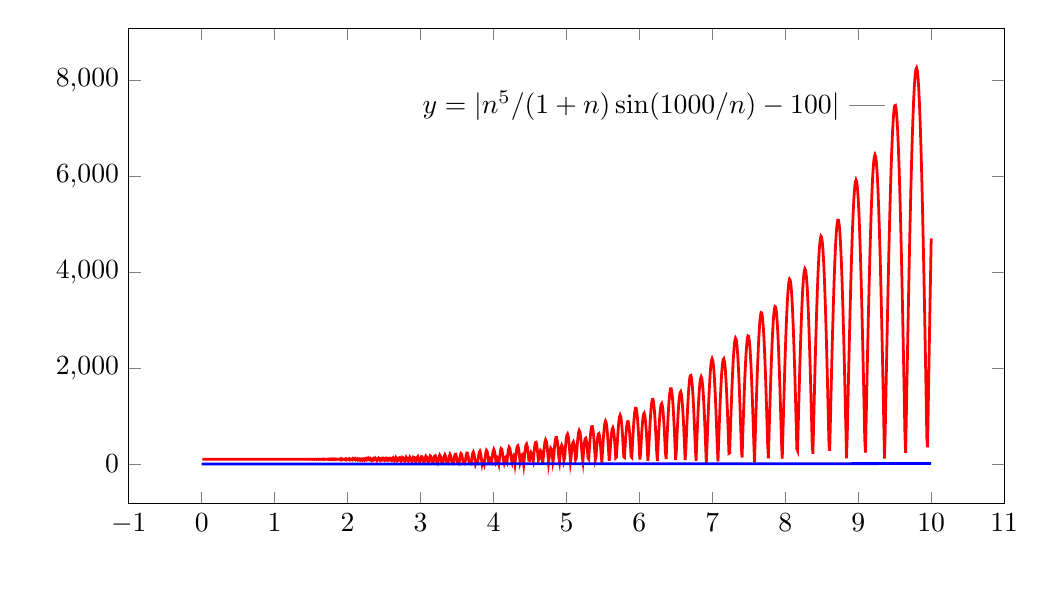
\begin{tikzpicture}[line width=1]
\begin{axis}[width=5in, height=3in,
             scatter/classes={a={mark=*,draw=black}},
             xlabel={\mbox{}},
             xlabel style={name=xlabel}, 
             ylabel={\mbox{}}, 
             legend style={
                at={(xlabel.south)},
                yshift=-1ex,
                anchor=north,
                legend cell align=left,
                },
        ]
]
\addplot[draw=red, line width=1] coordinates {(0.01,100.0)
(0.02,100.0)
(0.03,100.0)
(0.04,100.0)
(0.0501,100.0)
(0.0601,100.0)
(0.0701,100.0)
(0.0801,100.0)
(0.0901,100.0)
(0.1001,100.0)
(0.1101,100.0)
(0.1201,100.0)
(0.1301,100.0)
(0.1401,100.0)
(0.1502,100.0)
(0.1602,100.0001)
(0.1702,99.9999)
(0.1802,99.9999)
(0.1902,100.0002)
(0.2002,100.0)
(0.2102,99.9998)
(0.2202,100.0004)
(0.2302,99.9995)
(0.2402,99.9999)
(0.2503,100.0001)
(0.2603,100.0001)
(0.2703,100.0008)
(0.2803,100.0011)
(0.2903,99.9984)
(0.3003,100.0002)
(0.3103,100.0014)
(0.3203,100.0019)
(0.3303,100.0028)
(0.3403,100.0026)
(0.3504,99.9961)
(0.3604,100.0037)
(0.3704,100.005)
(0.3804,99.9969)
(0.3904,100.0059)
(0.4004,99.9995)
(0.4104,100.0079)
(0.4204,100.0035)
(0.4304,100.0103)
(0.4404,99.9909)
(0.4505,99.9886)
(0.4605,100.0111)
(0.4705,99.9848)
(0.4805,99.9827)
(0.4905,99.9978)
(0.5005,100.0011)
(0.5105,100.0229)
(0.5205,100.0251)
(0.5305,100.0014)
(0.5405,99.9884)
(0.5506,99.9837)
(0.5606,100.0169)
(0.5706,100.0142)
(0.5806,99.9695)
(0.5906,99.9956)
(0.6006,100.0022)
(0.6106,100.0424)
(0.6206,99.9807)
(0.6306,99.9565)
(0.6406,99.9723)
(0.6507,100.0447)
(0.6607,100.0435)
(0.6707,99.924)
(0.6807,100.0793)
(0.6907,99.9597)
(0.7007,99.9247)
(0.7107,100.0404)
(0.7207,100.0999)
(0.7307,100.1139)
(0.7407,100.0991)
(0.7508,100.0048)
(0.7608,99.861)
(0.7708,99.9885)
(0.7808,100.1372)
(0.7908,99.8277)
(0.8008,100.1828)
(0.8108,99.8129)
(0.8208,100.1231)
(0.8308,100.0811)
(0.8408,99.7759)
(0.8509,99.92)
(0.8609,100.1753)
(0.8709,100.2677)
(0.8809,100.2529)
(0.8909,100.2367)
(0.9009,100.2657)
(0.9109,100.3226)
(0.9209,100.3106)
(0.9309,100.083)
(0.9409,99.7005)
(0.951,99.6993)
(0.961,100.2872)
(0.971,100.2272)
(0.981,99.5422)
(0.991,100.2866)
(1.001,100.0133)
(1.011,99.7515)
(1.021,100.3803)
(1.031,99.5693)
(1.041,100.4085)
(1.0511,99.7145)
(1.0611,100.0163)
(1.0711,100.3797)
(1.0811,99.3044)
(1.0911,100.5463)
(1.1011,100.1992)
(1.1111,99.1996)
(1.1211,100.205)
(1.1311,100.8332)
(1.1411,99.8306)
(1.1512,99.0613)
(1.1612,99.6102)
(1.1712,100.6279)
(1.1812,101.0529)
(1.1912,100.6972)
(1.2012,99.9749)
(1.2112,99.316)
(1.2212,98.9084)
(1.2312,98.7374)
(1.2412,98.7051)
(1.2513,98.7135)
(1.2613,98.6972)
(1.2713,98.6291)
(1.2813,98.5218)
(1.2913,98.4333)
(1.3013,98.4725)
(1.3113,98.7831)
(1.3213,99.4779)
(1.3313,100.5081)
(1.3413,101.5244)
(1.3514,101.8936)
(1.3614,101.075)
(1.3714,99.3033)
(1.3814,97.9406)
(1.3914,98.5626)
(1.4014,100.9381)
(1.4114,102.315)
(1.4214,100.4658)
(1.4314,97.7263)
(1.4414,98.6852)
(1.4515,102.1477)
(1.4615,101.5752)
(1.4715,97.6395)
(1.4815,98.7688)
(1.4915,102.8627)
(1.5015,100.0538)
(1.5115,96.9846)
(1.5215,101.9416)
(1.5315,101.6252)
(1.5415,96.5773)
(1.5516,101.6573)
(1.5616,101.7388)
(1.5716,96.3051)
(1.5816,102.7984)
(1.5916,100.0656)
(1.6016,97.0887)
(1.6116,104.1607)
(1.6216,96.6112)
(1.6316,101.1842)
(1.6416,101.4311)
(1.6517,96.4487)
(1.6617,104.6718)
(1.6717,95.2906)
(1.6817,103.8715)
(1.6917,97.5104)
(1.7017,100.8896)
(1.7117,100.6794)
(1.7217,97.9346)
(1.7317,103.2022)
(1.7417,95.9153)
(1.7518,104.7427)
(1.7618,94.7808)
(1.7718,105.5553)
(1.7818,94.2201)
(1.7918,105.9045)
(1.8018,94.0809)
(1.8118,105.792)
(1.8218,94.5292)
(1.8318,104.8871)
(1.8418,96.0333)
(1.8519,102.6468)
(1.8619,99.0985)
(1.8719,98.7737)
(1.8819,103.5905)
(1.8919,94.0828)
(1.9019,107.8044)
(1.9119,91.2332)
(1.9219,108.3379)
(1.9319,93.7686)
(1.9419,102.5287)
(1.952,102.1706)
(1.962,93.268)
(1.972,109.6948)
(1.982,90.2638)
(1.992,106.3004)
(2.002,99.8583)
(2.012,93.4337)
(2.022,110.8471)
(2.032,89.7559)
(2.042,104.3574)
(2.0521,104.3135)
(2.0621,88.9055)
(2.0721,111.573)
(2.0821,95.3475)
(2.0921,94.1491)
(2.1021,112.8617)
(2.1121,89.2482)
(2.1221,100.1721)
(2.1321,111.165)
(2.1421,86.2686)
(2.1522,104.3922)
(2.1622,109.4646)
(2.1722,84.875)
(2.1822,106.2788)
(2.1922,109.388)
(2.2022,83.9634)
(2.2122,105.7045)
(2.2222,111.4917)
(2.2322,83.6447)
(2.2422,102.1623)
(2.2523,115.3265)
(2.2623,85.449)
(2.2723,95.1491)
(2.2823,118.7818)
(2.2923,91.8666)
(2.3023,85.839)
(2.3123,117.5281)
(2.3223,104.1439)
(2.3323,79.3426)
(2.3423,106.9063)
(2.3524,117.9793)
(2.3624,84.1523)
(2.3724,88.4371)
(2.3824,121.3509)
(2.3924,103.6763)
(2.4024,76.4811)
(2.4124,103.9897)
(2.4224,123.2152)
(2.4324,89.4886)
(2.4424,78.4954)
(2.4525,115.5909)
(2.4625,119.3337)
(2.4725,80.691)
(2.4825,82.5854)
(2.4925,121.8984)
(2.5025,116.2298)
(2.5125,76.4175)
(2.5225,83.9191)
(2.5325,124.476)
(2.5425,117.1332)
(2.5526,75.4692)
(2.5626,80.5715)
(2.5726,123.5181)
(2.5826,122.8565)
(2.5926,78.9562)
(2.6026,72.9149)
(2.6126,116.6155)
(2.6226,131.4681)
(2.6326,90.2189)
(2.6426,65.0309)
(2.6527,100.3591)
(2.6627,136.1652)
(2.6727,111.2488)
(2.6827,66.5771)
(2.6927,76.269)
(2.7027,125.3258)
(2.7127,134.6763)
(2.7227,88.6249)
(2.7327,59.2491)
(2.7427,92.829)
(2.7528,138.4801)
(2.7628,126.6767)
(2.7728,74.2894)
(2.7828,58.7105)
(2.7928,103.4479)
(2.8028,144.4373)
(2.8128,122.7875)
(2.8228,68.2253)
(2.8328,56.6493)
(2.8428,104.7187)
(2.8529,147.6561)
(2.8629,127.4459)
(2.8729,70.1016)
(2.8829,50.5877)
(2.8929,94.8274)
(2.9029,146.8884)
(2.9129,140.805)
(2.9229,83.3933)
(2.9329,45.056)
(2.9429,72.9663)
(2.953,134.2823)
(2.963,156.2209)
(2.973,112.3702)
(2.983,52.9834)
(2.993,46.2618)
(3.003,100.5382)
(3.013,155.5643)
(3.023,150.2114)
(3.033,89.593)
(3.043,38.7764)
(3.0531,52.357)
(3.0631,116.7428)
(3.0731,165.158)
(3.0831,147.3267)
(3.0931,80.6805)
(3.1031,31.9667)
(3.1131,50.034)
(3.1231,117.8389)
(3.1331,169.8365)
(3.1431,155.726)
(3.1532,88.1914)
(3.1632,30.2144)
(3.1732,35.861)
(3.1832,100.6502)
(3.1932,166.3266)
(3.2032,173.8673)
(3.2132,115.9348)
(3.2232,42.7)
(3.2332,17.5855)
(3.2432,62.665)
(3.2533,140.4329)
(3.2633,185.9931)
(3.2733,161.2194)
(3.2833,85.6927)
(3.2933,20.1203)
(3.3033,17.1679)
(3.3133,79.8156)
(3.3233,159.6335)
(3.3333,194.9436)
(3.3433,158.2441)
(3.3534,76.6251)
(3.3634,10.7952)
(3.3734,9.6847)
(3.3834,74.739)
(3.3934,159.4614)
(3.4034,203.329)
(3.4134,174.8611)
(3.4234,93.3229)
(3.4334,14.7371)
(3.4434,6.9867)
(3.4535,43.415)
(3.4635,132.8045)
(3.4735,202.2344)
(3.4835,205.9565)
(3.4935,140.9551)
(3.5035,48.3478)
(3.5135,13.2874)
(3.5235,4.9412)
(3.5335,68.8218)
(3.5435,163.2172)
(3.5536,220.9944)
(3.5636,207.0542)
(3.5736,129.0734)
(3.5836,32.4443)
(3.5936,26.6619)
(3.6036,13.8306)
(3.6136,64.2283)
(3.6236,163.9863)
(3.6336,229.8827)
(3.6436,225.1968)
(3.6537,151.9038)
(3.6637,49.1185)
(3.6737,28.3288)
(3.6837,39.1637)
(3.6937,22.8438)
(3.7037,126.0836)
(3.7137,217.8269)
(3.7237,251.3134)
(3.7337,209.2176)
(3.7437,111.9136)
(3.7538,6.9539)
(3.7638,54.4841)
(3.7738,42.3722)
(3.7838,38.071)
(3.7938,149.2919)
(3.8038,239.4049)
(3.8138,266.4424)
(3.8238,217.5042)
(3.8338,114.2599)
(3.8438,2.7648)
(3.8539,67.3644)
(3.8639,64.8811)
(3.8739,9.6737)
(3.8839,124.6003)
(3.8939,230.9981)
(3.9039,283.706)
(3.9139,260.2091)
(3.9239,169.7138)
(3.9339,48.9672)
(3.9439,53.0556)
(3.954,95.06)
(3.964,59.8343)
(3.974,39.239)
(3.984,163.8028)
(3.994,265.7136)
(4.004,305.6579)
(4.014,268.0019)
(4.024,166.3913)
(4.034,38.2997)
(4.044,69.1136)
(4.0541,116.3856)
(4.0641,85.9629)
(4.0741,11.7625)
(4.0841,142.4905)
(4.0941,260.3889)
(4.1041,324.2276)
(4.1141,311.5746)
(4.1241,226.2484)
(4.1341,96.7038)
(4.1441,33.8274)
(4.1542,121.9046)
(4.1642,138.2051)
(4.1742,76.9314)
(4.1842,42.5969)
(4.1942,182.4395)
(4.2042,298.3106)
(4.2142,353.5915)
(4.2242,330.6551)
(4.2342,236.0829)
(4.2442,98.3609)
(4.2543,41.0217)
(4.2643,140.194)
(4.2743,169.3743)
(4.2843,119.5117)
(4.2943,4.685)
(4.3043,142.2508)
(4.3143,279.3187)
(4.3243,367.4679)
(4.3343,381.547)
(4.3443,317.1653)
(4.3544,191.6625)
(4.3644,39.0954)
(4.3744,99.2193)
(4.3844,185.9235)
(4.3944,197.5483)
(4.4044,130.5626)
(4.4144,2.0652)
(4.4244,154.9025)
(4.4344,300.0578)
(4.4444,396.2519)
(4.4545,418.8378)
(4.4645,361.7112)
(4.4745,238.6124)
(4.4845,79.5078)
(4.4945,76.923)
(4.5045,192.7602)
(4.5145,239.9437)
(4.5245,206.8396)
(4.5345,100.7975)
(4.5445,53.7886)
(4.5546,221.3355)
(4.5646,363.3827)
(4.5746,447.3955)
(4.5846,454.0514)
(4.5946,381.4195)
(4.6046,245.1909)
(4.6146,75.0207)
(4.6246,92.1093)
(4.6346,219.9834)
(4.6446,280.9209)
(4.6547,261.5729)
(4.6647,165.5791)
(4.6747,12.6129)
(4.6847,165.8837)
(4.6947,333.3053)
(4.7047,455.4141)
(4.7147,507.2435)
(4.7247,478.0062)
(4.7347,373.0822)
(4.7447,212.7758)
(4.7548,28.1733)
(4.7648,145.0128)
(4.7748,273.3724)
(4.7848,332.1524)
(4.7948,309.8484)
(4.8048,210.2191)
(4.8148,51.4161)
(4.8248,137.5289)
(4.8348,322.1453)
(4.8448,468.85)
(4.8549,550.9924)
(4.8649,553.5444)
(4.8749,475.6387)
(4.8849,330.5656)
(4.8949,143.2986)
(4.9049,53.9576)
(4.9149,227.3763)
(4.9249,347.2903)
(4.9349,393.1595)
(4.9449,356.9155)
(4.955,244.1682)
(4.965,73.1315)
(4.975,128.4941)
(4.985,328.1222)
(4.995,493.5829)
(5.005,598.2596)
(5.015,625.2496)
(5.025,569.9188)
(5.035,440.4934)
(5.045,256.6479)
(5.0551,46.3603)
(5.0651,158.4425)
(5.0751,326.7551)
(5.0851,433.1376)
(5.0951,461.4444)
(5.1051,407.1111)
(5.1151,277.7012)
(5.1251,91.677)
(5.1351,124.3808)
(5.1451,339.6664)
(5.1552,523.5725)
(5.1652,650.0059)
(5.1752,700.992)
(5.1852,669.0871)
(5.1952,558.2938)
(5.2052,383.3936)
(5.2152,167.8279)
(5.2252,59.5512)
(5.2352,268.3947)
(5.2452,430.9003)
(5.2553,525.4468)
(5.2653,539.3571)
(5.2753,470.4494)
(5.2853,327.2099)
(5.2953,127.5982)
(5.3053,103.3283)
(5.3153,336.642)
(5.3253,543.1995)
(5.3353,697.2584)
(5.3453,779.6115)
(5.3554,779.8667)
(5.3654,697.6176)
(5.3754,542.3905)
(5.3854,332.4048)
(5.3954,92.3232)
(5.4054,149.718)
(5.4154,365.4332)
(5.4254,529.6712)
(5.4354,623.2809)
(5.4454,635.2404)
(5.4555,563.8268)
(5.4655,416.7162)
(5.4755,210.0311)
(5.4855,33.536)
(5.4955,287.2897)
(5.5055,523.495)
(5.5155,716.4016)
(5.5255,845.003)
(5.5355,895.2392)
(5.5455,861.4236)
(5.5556,746.7601)
(5.5656,562.9189)
(5.5756,328.7378)
(5.5856,68.2046)
(5.5956,192.0561)
(5.6056,425.5216)
(5.6156,608.4537)
(5.6256,722.2564)
(5.6356,755.2801)
(5.6456,703.9079)
(5.6557,572.8322)
(5.6657,374.516)
(5.6757,127.9074)
(5.6857,143.4476)
(5.6957,413.702)
(5.7057,657.1849)
(5.7157,850.8205)
(5.7257,976.2641)
(5.7357,1021.5625)
(5.7457,982.1965)
(5.7558,861.4232)
(5.7658,669.9049)
(5.7758,424.6732)
(5.7858,147.5376)
(5.7958,136.9059)
(5.8058,403.4815)
(5.8158,628.6542)
(5.8258,792.5717)
(5.8358,880.7525)
(5.8458,885.2833)
(5.8559,805.4341)
(5.8659,647.6526)
(5.8759,424.9509)
(5.8859,155.7521)
(5.8959,137.6967)
(5.9059,431.2014)
(5.9159,700.6293)
(5.9259,923.8786)
(5.9359,1082.6529)
(5.9459,1163.8995)
(5.956,1160.805)
(5.966,1073.2786)
(5.976,907.8968)
(5.986,677.3248)
(5.996,399.2733)
(6.006,95.0801)
(6.016,211.9644)
(6.026,498.4143)
(6.036,742.4492)
(6.046,925.5042)
(6.0561,1033.6299)
(6.0661,1058.4883)
(6.0761,997.9168)
(6.0861,856.0307)
(6.0961,642.8651)
(6.1061,373.5935)
(6.1161,67.3878)
(6.1261,253.9891)
(6.1361,567.7541)
(6.1461,851.7221)
(6.1562,1085.8563)
(6.1662,1253.6457)
(6.1762,1343.2166)
(6.1862,1348.1071)
(6.1962,1267.6603)
(6.2062,1107.0161)
(6.2162,876.7122)
(6.2262,591.9288)
(6.2362,271.4353)
(6.2462,63.6846)
(6.2563,391.4404)
(6.2663,690.3803)
(6.2763,940.9798)
(6.2863,1126.8847)
(6.2963,1235.931)
(6.3063,1260.883)
(6.3163,1199.8477)
(6.3263,1056.3463)
(6.3363,839.0459)
(6.3463,561.1756)
(6.3564,239.6689)
(6.3664,105.9074)
(6.3764,454.5703)
(6.3864,785.2036)
(6.3964,1077.8314)
(6.4064,1314.8029)
(6.4164,1481.822)
(6.4264,1568.7624)
(6.4364,1570.2264)
(6.4464,1485.8181)
(6.4565,1320.1229)
(6.4665,1082.3998)
(6.4765,786.0103)
(6.4865,447.6213)
(6.4965,86.2338)
(6.5065,277.9063)
(6.5165,624.4512)
(6.5265,934.0821)
(6.5365,1189.5674)
(6.5465,1376.6908)
(6.5566,1485.0002)
(6.5666,1508.3429)
(6.5766,1445.1595)
(6.5866,1298.5285)
(6.5966,1075.9625)
(6.6066,788.9728)
(6.6166,452.4296)
(6.6266,83.756)
(6.6366,297.9995)
(6.6466,673.1604)
(6.6567,1022.4384)
(6.6667,1327.9144)
(6.6767,1573.9362)
(6.6867,1747.8884)
(6.6967,1840.7998)
(6.7067,1847.7589)
(6.7167,1768.1241)
(6.7267,1605.5182)
(6.7367,1367.616)
(6.7467,1065.7367)
(6.7568,714.2655)
(6.7668,329.9361)
(6.7768,68.9885)
(6.7868,463.5974)
(6.7968,835.2301)
(6.8068,1166.3514)
(6.8168,1441.3606)
(6.8268,1647.3)
(6.8368,1774.4306)
(6.8468,1816.6526)
(6.8569,1771.7533)
(6.8669,1641.4757)
(6.8769,1431.407)
(6.8869,1150.6966)
(6.8969,811.619)
(6.9069,429.0041)
(6.9169,19.5631)
(6.9269,398.8589)
(6.9369,808.0693)
(6.9469,1190.3187)
(6.957,1529.0612)
(6.967,1809.653)
(6.977,2019.9598)
(6.987,2150.8501)
(6.997,2196.5552)
(7.007,2154.8827)
(7.017,2027.2793)
(7.027,1818.741)
(7.037,1537.5795)
(7.047,1195.0553)
(7.0571,804.8959)
(7.0671,382.7213)
(7.0771,54.5992)
(7.0871,489.6318)
(7.0971,905.0753)
(7.1071,1284.444)
(7.1171,1612.7094)
(7.1271,1876.8756)
(7.1371,2066.4685)
(7.1471,2173.9204)
(7.1572,2194.8377)
(7.1672,2128.1438)
(7.1772,1976.0935)
(7.1872,1744.1613)
(7.1972,1440.8107)
(7.2072,1077.1534)
(7.2172,666.516)
(7.2272,223.9298)
(7.2372,234.4355)
(7.2472,691.8714)
(7.2573,1131.743)
(7.2673,1538.0891)
(7.2773,1896.1916)
(7.2873,2193.0916)
(7.2973,2418.0368)
(7.3073,2562.8448)
(7.3173,2622.1705)
(7.3273,2593.6712)
(7.3373,2478.0649)
(7.3473,2279.0816)
(7.3574,2003.3115)
(7.3674,1659.9574)
(7.3774,1260.5008)
(7.3874,818.296)
(7.3974,348.1055)
(7.4074,134.4053)
(7.4174,613.197)
(7.4274,1072.3903)
(7.4374,1496.789)
(7.4474,1872.3719)
(7.4575,2186.7417)
(7.4675,2429.5146)
(7.4775,2592.6398)
(7.4875,2670.6399)
(7.4975,2660.7665)
(7.5075,2563.0662)
(7.5175,2380.3582)
(7.5275,2118.1249)
(7.5375,1784.3197)
(7.5475,1389.1018)
(7.5576,944.5052)
(7.5676,464.0542)
(7.5776,37.6612)
(7.5876,545.4374)
(7.5976,1043.9219)
(7.6076,1518.0771)
(7.6176,1953.6277)
(7.6276,2337.4809)
(7.6376,2658.1053)
(7.6476,2905.8591)
(7.6577,3073.2591)
(7.6677,3155.1827)
(7.6777,3148.999)
(7.6877,3054.6262)
(7.6977,2874.5152)
(7.7077,2613.5606)
(7.7177,2278.9431)
(7.7277,1879.9103)
(7.7377,1427.5004)
(7.7477,934.2203)
(7.7578,413.6868)
(7.7678,119.7591)
(7.7778,651.4529)
(7.7878,1166.8108)
(7.7978,1651.7267)
(7.8078,2092.9521)
(7.8178,2478.4471)
(7.8278,2797.6951)
(7.8378,3041.9724)
(7.8478,3204.5675)
(7.8579,3280.9439)
(7.8679,3268.8431)
(7.8779,3168.328)
(7.8879,2981.7636)
(7.8979,2713.7394)
(7.9079,2370.9351)
(7.9179,1961.9334)
(7.9279,1496.9877)
(7.9379,987.7496)
(7.9479,446.9637)
(7.958,111.86)
(7.968,674.79)
(7.978,1227.8233)
(7.988,1757.2324)
(7.998,2249.9018)
(8.008,2693.6456)
(8.018,3077.4974)
(8.028,3391.9688)
(8.038,3629.2672)
(8.048,3783.4716)
(8.0581,3850.6607)
(8.0681,3828.9918)
(8.0781,3718.7302)
(8.0881,3522.2273)
(8.0981,3243.8511)
(8.1081,2889.8701)
(8.1181,2468.2937)
(8.1281,1988.6756)
(8.1381,1461.8826)
(8.1481,899.8372)
(8.1582,315.2384)
(8.1682,278.7313)
(8.1782,868.7064)
(8.1882,1441.4397)
(8.1982,1984.0972)
(8.2082,2484.5402)
(8.2182,2931.5888)
(8.2282,3315.2613)
(8.2382,3626.9842)
(8.2482,3859.7693)
(8.2583,4008.3543)
(8.2683,4069.3038)
(8.2783,4041.071)
(8.2883,3924.0174)
(8.2983,3720.3917)
(8.3083,3434.2696)
(8.3183,3071.4548)
(8.3283,2639.3457)
(8.3383,2146.77)
(8.3483,1603.7917)
(8.3584,1021.4945)
(8.3684,411.7469)
(8.3784,213.046)
(8.3884,840.199)
(8.3984,1457.0054)
(8.4084,2050.9941)
(8.4184,2610.1779)
(8.4284,3123.2898)
(8.4384,3580.0025)
(8.4484,3971.1259)
(8.4585,4288.7808)
(8.4685,4526.5441)
(8.4785,4679.5647)
(8.4885,4744.6465)
(8.4985,4720.2997)
(8.5085,4606.7571)
(8.5185,4405.9584)
(8.5285,4121.502)
(8.5385,3758.5647)
(8.5485,3323.7943)
(8.5586,2825.1741)
(8.5686,2271.8646)
(8.5786,1674.0256)
(8.5886,1042.6205)
(8.5986,389.2092)
(8.6086,274.2684)
(8.6186,935.713)
(8.6286,1583.0872)
(8.6386,2204.6326)
(8.6486,2789.0806)
(8.6587,3325.8505)
(8.6687,3805.2345)
(8.6787,4218.5638)
(8.6887,4558.3557)
(8.6987,4818.437)
(8.7087,4994.0438)
(8.7187,5081.8954)
(8.7287,5080.2412)
(8.7387,4988.8809)
(8.7487,4809.1581)
(8.7588,4543.9264)
(8.7688,4197.4917)
(8.7788,3775.5288)
(8.7888,3284.9769)
(8.7988,2733.9144)
(8.8088,2131.4163)
(8.8188,1487.3963)
(8.8288,812.4369)
(8.8388,117.6102)
(8.8488,585.7074)
(8.8589,1286.0235)
(8.8689,1971.9175)
(8.8789,2632.2255)
(8.8889,3256.2192)
(8.8989,3833.7751)
(8.9089,4355.5328)
(8.9189,4813.0394)
(8.9289,5198.8771)
(8.9389,5506.7746)
(8.9489,5731.6974)
(8.959,5869.9189)
(8.969,5919.0703)
(8.979,5878.1682)
(8.989,5747.6213)
(8.999,5529.2146)
(9.009,5226.074)
(9.019,4842.6093)
(9.029,4384.4398)
(9.039,3858.3012)
(9.049,3271.9374)
(9.0591,2633.9782)
(9.0691,1953.8049)
(9.0791,1241.4065)
(9.0891,507.228)
(9.0991,237.9858)
(9.1091,983.3496)
(9.1191,1717.9973)
(9.1291,2431.2395)
(9.1391,3112.7168)
(9.1491,3752.5469)
(9.1592,4341.4631)
(9.1692,4870.9425)
(9.1792,5333.3222)
(9.1892,5721.9027)
(9.1992,6031.0355)
(9.2092,6256.1964)
(9.2192,6394.0408)
(9.2292,6442.4435)
(9.2392,6400.5198)
(9.2492,6268.6306)
(9.2593,6048.3689)
(9.2693,5742.531)
(9.2793,5355.071)
(9.2893,4891.0393)
(9.2993,4356.5085)
(9.3093,3758.4852)
(9.3193,3104.8108)
(9.3293,2404.0514)
(9.3393,1665.3806)
(9.3493,898.4541)
(9.3594,113.2802)
(9.3694,679.9134)
(9.3794,1470.8142)
(9.3894,2249.159)
(9.3994,3004.8663)
(9.4094,3728.1648)
(9.4194,4409.7164)
(9.4294,5040.733)
(9.4394,5613.0843)
(9.4494,6119.3966)
(9.4595,6553.1412)
(9.4695,6908.7112)
(9.4795,7181.4852)
(9.4895,7367.8793)
(9.4995,7465.3852)
(9.5095,7472.594)
(9.5195,7389.2074)
(9.5295,7216.034)
(9.5395,6954.9736)
(9.5495,6608.9865)
(9.5596,6182.0521)
(9.5696,5679.1147)
(9.5796,5106.0185)
(9.5896,4469.4322)
(9.5996,3776.7655)
(9.6096,3036.0765)
(9.6196,2255.9732)
(9.6296,1445.5093)
(9.6396,614.0757)
(9.6496,228.7105)
(9.6597,1073.1189)
(9.6697,1909.4183)
(9.6797,2727.9888)
(9.6897,3519.4309)
(9.6997,4274.6713)
(9.7097,4985.0636)
(9.7197,5642.4839)
(9.7297,6239.4183)
(9.7397,6769.0442)
(9.7497,7225.3016)
(9.7598,7602.9564)
(9.7698,7897.6532)
(9.7798,8105.9578)
(9.7898,8225.3899)
(9.7998,8254.4442)
(9.8098,8192.6014)
(9.8198,8040.3273)
(9.8298,7799.0629)
(9.8398,7471.2023)
(9.8498,7060.0619)
(9.8599,6569.8398)
(9.8699,6005.5653)
(9.8799,5373.0417)
(9.8899,4678.78)
(9.8999,3929.9268)
(9.9099,3134.1856)
(9.9199,2299.7338)
(9.9299,1435.1346)
(9.9399,549.2471)
(9.9499,348.8674)
(9.96,1250.0385)
(9.97,2145.0815)
(9.98,3024.8905)
(9.99,3880.5299)
(10.0,4703.324)
(10.0,4703.324)};\node[pin=left:{$y=|n^5/(1 + n)   \sin(1000/n) - 100|$}] at (axis cs:9.5,7467.8971870303885) {};\addplot[draw=blue, line width=1] coordinates {(0.0,0.0)
(5.0,5.0)
(10.0,10.0)
(10.0,10.0)};
\end{axis}\end{tikzpicture}\end{center}


With $g(n) = n^2$:
%-*-latex-*-

\begin{center}
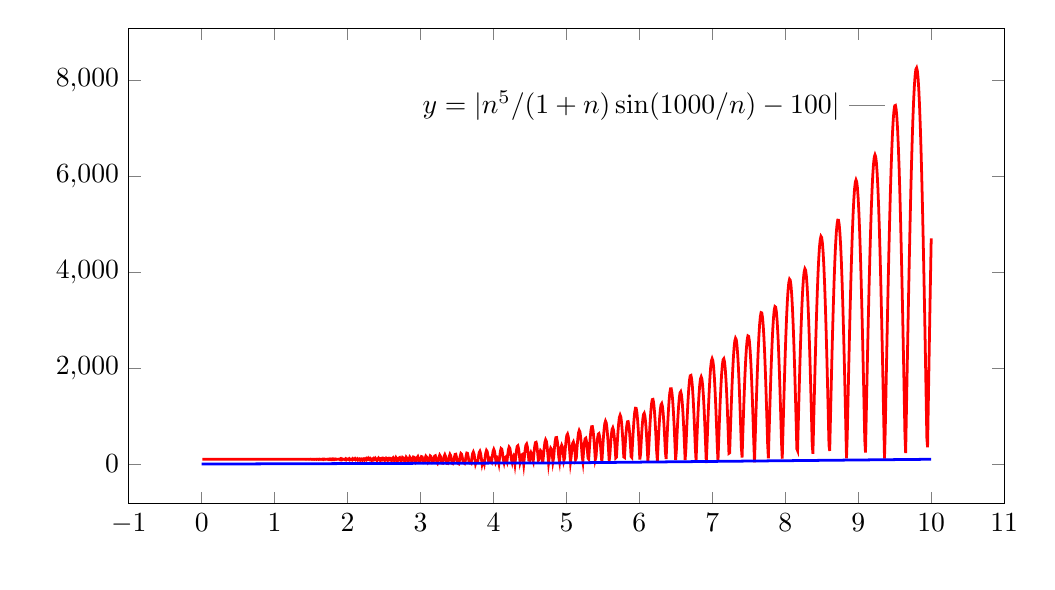
\begin{tikzpicture}[line width=1]
\begin{axis}[width=5in, height=3in,
             scatter/classes={a={mark=*,draw=black}},
             xlabel={\mbox{}},
             xlabel style={name=xlabel}, 
             ylabel={\mbox{}}, 
             legend style={
                at={(xlabel.south)},
                yshift=-1ex,
                anchor=north,
                legend cell align=left,
                },
        ]
]
\addplot[draw=red, line width=1] coordinates {(0.01,100.0)
(0.02,100.0)
(0.03,100.0)
(0.04,100.0)
(0.0501,100.0)
(0.0601,100.0)
(0.0701,100.0)
(0.0801,100.0)
(0.0901,100.0)
(0.1001,100.0)
(0.1101,100.0)
(0.1201,100.0)
(0.1301,100.0)
(0.1401,100.0)
(0.1502,100.0)
(0.1602,100.0001)
(0.1702,99.9999)
(0.1802,99.9999)
(0.1902,100.0002)
(0.2002,100.0)
(0.2102,99.9998)
(0.2202,100.0004)
(0.2302,99.9995)
(0.2402,99.9999)
(0.2503,100.0001)
(0.2603,100.0001)
(0.2703,100.0008)
(0.2803,100.0011)
(0.2903,99.9984)
(0.3003,100.0002)
(0.3103,100.0014)
(0.3203,100.0019)
(0.3303,100.0028)
(0.3403,100.0026)
(0.3504,99.9961)
(0.3604,100.0037)
(0.3704,100.005)
(0.3804,99.9969)
(0.3904,100.0059)
(0.4004,99.9995)
(0.4104,100.0079)
(0.4204,100.0035)
(0.4304,100.0103)
(0.4404,99.9909)
(0.4505,99.9886)
(0.4605,100.0111)
(0.4705,99.9848)
(0.4805,99.9827)
(0.4905,99.9978)
(0.5005,100.0011)
(0.5105,100.0229)
(0.5205,100.0251)
(0.5305,100.0014)
(0.5405,99.9884)
(0.5506,99.9837)
(0.5606,100.0169)
(0.5706,100.0142)
(0.5806,99.9695)
(0.5906,99.9956)
(0.6006,100.0022)
(0.6106,100.0424)
(0.6206,99.9807)
(0.6306,99.9565)
(0.6406,99.9723)
(0.6507,100.0447)
(0.6607,100.0435)
(0.6707,99.924)
(0.6807,100.0793)
(0.6907,99.9597)
(0.7007,99.9247)
(0.7107,100.0404)
(0.7207,100.0999)
(0.7307,100.1139)
(0.7407,100.0991)
(0.7508,100.0048)
(0.7608,99.861)
(0.7708,99.9885)
(0.7808,100.1372)
(0.7908,99.8277)
(0.8008,100.1828)
(0.8108,99.8129)
(0.8208,100.1231)
(0.8308,100.0811)
(0.8408,99.7759)
(0.8509,99.92)
(0.8609,100.1753)
(0.8709,100.2677)
(0.8809,100.2529)
(0.8909,100.2367)
(0.9009,100.2657)
(0.9109,100.3226)
(0.9209,100.3106)
(0.9309,100.083)
(0.9409,99.7005)
(0.951,99.6993)
(0.961,100.2872)
(0.971,100.2272)
(0.981,99.5422)
(0.991,100.2866)
(1.001,100.0133)
(1.011,99.7515)
(1.021,100.3803)
(1.031,99.5693)
(1.041,100.4085)
(1.0511,99.7145)
(1.0611,100.0163)
(1.0711,100.3797)
(1.0811,99.3044)
(1.0911,100.5463)
(1.1011,100.1992)
(1.1111,99.1996)
(1.1211,100.205)
(1.1311,100.8332)
(1.1411,99.8306)
(1.1512,99.0613)
(1.1612,99.6102)
(1.1712,100.6279)
(1.1812,101.0529)
(1.1912,100.6972)
(1.2012,99.9749)
(1.2112,99.316)
(1.2212,98.9084)
(1.2312,98.7374)
(1.2412,98.7051)
(1.2513,98.7135)
(1.2613,98.6972)
(1.2713,98.6291)
(1.2813,98.5218)
(1.2913,98.4333)
(1.3013,98.4725)
(1.3113,98.7831)
(1.3213,99.4779)
(1.3313,100.5081)
(1.3413,101.5244)
(1.3514,101.8936)
(1.3614,101.075)
(1.3714,99.3033)
(1.3814,97.9406)
(1.3914,98.5626)
(1.4014,100.9381)
(1.4114,102.315)
(1.4214,100.4658)
(1.4314,97.7263)
(1.4414,98.6852)
(1.4515,102.1477)
(1.4615,101.5752)
(1.4715,97.6395)
(1.4815,98.7688)
(1.4915,102.8627)
(1.5015,100.0538)
(1.5115,96.9846)
(1.5215,101.9416)
(1.5315,101.6252)
(1.5415,96.5773)
(1.5516,101.6573)
(1.5616,101.7388)
(1.5716,96.3051)
(1.5816,102.7984)
(1.5916,100.0656)
(1.6016,97.0887)
(1.6116,104.1607)
(1.6216,96.6112)
(1.6316,101.1842)
(1.6416,101.4311)
(1.6517,96.4487)
(1.6617,104.6718)
(1.6717,95.2906)
(1.6817,103.8715)
(1.6917,97.5104)
(1.7017,100.8896)
(1.7117,100.6794)
(1.7217,97.9346)
(1.7317,103.2022)
(1.7417,95.9153)
(1.7518,104.7427)
(1.7618,94.7808)
(1.7718,105.5553)
(1.7818,94.2201)
(1.7918,105.9045)
(1.8018,94.0809)
(1.8118,105.792)
(1.8218,94.5292)
(1.8318,104.8871)
(1.8418,96.0333)
(1.8519,102.6468)
(1.8619,99.0985)
(1.8719,98.7737)
(1.8819,103.5905)
(1.8919,94.0828)
(1.9019,107.8044)
(1.9119,91.2332)
(1.9219,108.3379)
(1.9319,93.7686)
(1.9419,102.5287)
(1.952,102.1706)
(1.962,93.268)
(1.972,109.6948)
(1.982,90.2638)
(1.992,106.3004)
(2.002,99.8583)
(2.012,93.4337)
(2.022,110.8471)
(2.032,89.7559)
(2.042,104.3574)
(2.0521,104.3135)
(2.0621,88.9055)
(2.0721,111.573)
(2.0821,95.3475)
(2.0921,94.1491)
(2.1021,112.8617)
(2.1121,89.2482)
(2.1221,100.1721)
(2.1321,111.165)
(2.1421,86.2686)
(2.1522,104.3922)
(2.1622,109.4646)
(2.1722,84.875)
(2.1822,106.2788)
(2.1922,109.388)
(2.2022,83.9634)
(2.2122,105.7045)
(2.2222,111.4917)
(2.2322,83.6447)
(2.2422,102.1623)
(2.2523,115.3265)
(2.2623,85.449)
(2.2723,95.1491)
(2.2823,118.7818)
(2.2923,91.8666)
(2.3023,85.839)
(2.3123,117.5281)
(2.3223,104.1439)
(2.3323,79.3426)
(2.3423,106.9063)
(2.3524,117.9793)
(2.3624,84.1523)
(2.3724,88.4371)
(2.3824,121.3509)
(2.3924,103.6763)
(2.4024,76.4811)
(2.4124,103.9897)
(2.4224,123.2152)
(2.4324,89.4886)
(2.4424,78.4954)
(2.4525,115.5909)
(2.4625,119.3337)
(2.4725,80.691)
(2.4825,82.5854)
(2.4925,121.8984)
(2.5025,116.2298)
(2.5125,76.4175)
(2.5225,83.9191)
(2.5325,124.476)
(2.5425,117.1332)
(2.5526,75.4692)
(2.5626,80.5715)
(2.5726,123.5181)
(2.5826,122.8565)
(2.5926,78.9562)
(2.6026,72.9149)
(2.6126,116.6155)
(2.6226,131.4681)
(2.6326,90.2189)
(2.6426,65.0309)
(2.6527,100.3591)
(2.6627,136.1652)
(2.6727,111.2488)
(2.6827,66.5771)
(2.6927,76.269)
(2.7027,125.3258)
(2.7127,134.6763)
(2.7227,88.6249)
(2.7327,59.2491)
(2.7427,92.829)
(2.7528,138.4801)
(2.7628,126.6767)
(2.7728,74.2894)
(2.7828,58.7105)
(2.7928,103.4479)
(2.8028,144.4373)
(2.8128,122.7875)
(2.8228,68.2253)
(2.8328,56.6493)
(2.8428,104.7187)
(2.8529,147.6561)
(2.8629,127.4459)
(2.8729,70.1016)
(2.8829,50.5877)
(2.8929,94.8274)
(2.9029,146.8884)
(2.9129,140.805)
(2.9229,83.3933)
(2.9329,45.056)
(2.9429,72.9663)
(2.953,134.2823)
(2.963,156.2209)
(2.973,112.3702)
(2.983,52.9834)
(2.993,46.2618)
(3.003,100.5382)
(3.013,155.5643)
(3.023,150.2114)
(3.033,89.593)
(3.043,38.7764)
(3.0531,52.357)
(3.0631,116.7428)
(3.0731,165.158)
(3.0831,147.3267)
(3.0931,80.6805)
(3.1031,31.9667)
(3.1131,50.034)
(3.1231,117.8389)
(3.1331,169.8365)
(3.1431,155.726)
(3.1532,88.1914)
(3.1632,30.2144)
(3.1732,35.861)
(3.1832,100.6502)
(3.1932,166.3266)
(3.2032,173.8673)
(3.2132,115.9348)
(3.2232,42.7)
(3.2332,17.5855)
(3.2432,62.665)
(3.2533,140.4329)
(3.2633,185.9931)
(3.2733,161.2194)
(3.2833,85.6927)
(3.2933,20.1203)
(3.3033,17.1679)
(3.3133,79.8156)
(3.3233,159.6335)
(3.3333,194.9436)
(3.3433,158.2441)
(3.3534,76.6251)
(3.3634,10.7952)
(3.3734,9.6847)
(3.3834,74.739)
(3.3934,159.4614)
(3.4034,203.329)
(3.4134,174.8611)
(3.4234,93.3229)
(3.4334,14.7371)
(3.4434,6.9867)
(3.4535,43.415)
(3.4635,132.8045)
(3.4735,202.2344)
(3.4835,205.9565)
(3.4935,140.9551)
(3.5035,48.3478)
(3.5135,13.2874)
(3.5235,4.9412)
(3.5335,68.8218)
(3.5435,163.2172)
(3.5536,220.9944)
(3.5636,207.0542)
(3.5736,129.0734)
(3.5836,32.4443)
(3.5936,26.6619)
(3.6036,13.8306)
(3.6136,64.2283)
(3.6236,163.9863)
(3.6336,229.8827)
(3.6436,225.1968)
(3.6537,151.9038)
(3.6637,49.1185)
(3.6737,28.3288)
(3.6837,39.1637)
(3.6937,22.8438)
(3.7037,126.0836)
(3.7137,217.8269)
(3.7237,251.3134)
(3.7337,209.2176)
(3.7437,111.9136)
(3.7538,6.9539)
(3.7638,54.4841)
(3.7738,42.3722)
(3.7838,38.071)
(3.7938,149.2919)
(3.8038,239.4049)
(3.8138,266.4424)
(3.8238,217.5042)
(3.8338,114.2599)
(3.8438,2.7648)
(3.8539,67.3644)
(3.8639,64.8811)
(3.8739,9.6737)
(3.8839,124.6003)
(3.8939,230.9981)
(3.9039,283.706)
(3.9139,260.2091)
(3.9239,169.7138)
(3.9339,48.9672)
(3.9439,53.0556)
(3.954,95.06)
(3.964,59.8343)
(3.974,39.239)
(3.984,163.8028)
(3.994,265.7136)
(4.004,305.6579)
(4.014,268.0019)
(4.024,166.3913)
(4.034,38.2997)
(4.044,69.1136)
(4.0541,116.3856)
(4.0641,85.9629)
(4.0741,11.7625)
(4.0841,142.4905)
(4.0941,260.3889)
(4.1041,324.2276)
(4.1141,311.5746)
(4.1241,226.2484)
(4.1341,96.7038)
(4.1441,33.8274)
(4.1542,121.9046)
(4.1642,138.2051)
(4.1742,76.9314)
(4.1842,42.5969)
(4.1942,182.4395)
(4.2042,298.3106)
(4.2142,353.5915)
(4.2242,330.6551)
(4.2342,236.0829)
(4.2442,98.3609)
(4.2543,41.0217)
(4.2643,140.194)
(4.2743,169.3743)
(4.2843,119.5117)
(4.2943,4.685)
(4.3043,142.2508)
(4.3143,279.3187)
(4.3243,367.4679)
(4.3343,381.547)
(4.3443,317.1653)
(4.3544,191.6625)
(4.3644,39.0954)
(4.3744,99.2193)
(4.3844,185.9235)
(4.3944,197.5483)
(4.4044,130.5626)
(4.4144,2.0652)
(4.4244,154.9025)
(4.4344,300.0578)
(4.4444,396.2519)
(4.4545,418.8378)
(4.4645,361.7112)
(4.4745,238.6124)
(4.4845,79.5078)
(4.4945,76.923)
(4.5045,192.7602)
(4.5145,239.9437)
(4.5245,206.8396)
(4.5345,100.7975)
(4.5445,53.7886)
(4.5546,221.3355)
(4.5646,363.3827)
(4.5746,447.3955)
(4.5846,454.0514)
(4.5946,381.4195)
(4.6046,245.1909)
(4.6146,75.0207)
(4.6246,92.1093)
(4.6346,219.9834)
(4.6446,280.9209)
(4.6547,261.5729)
(4.6647,165.5791)
(4.6747,12.6129)
(4.6847,165.8837)
(4.6947,333.3053)
(4.7047,455.4141)
(4.7147,507.2435)
(4.7247,478.0062)
(4.7347,373.0822)
(4.7447,212.7758)
(4.7548,28.1733)
(4.7648,145.0128)
(4.7748,273.3724)
(4.7848,332.1524)
(4.7948,309.8484)
(4.8048,210.2191)
(4.8148,51.4161)
(4.8248,137.5289)
(4.8348,322.1453)
(4.8448,468.85)
(4.8549,550.9924)
(4.8649,553.5444)
(4.8749,475.6387)
(4.8849,330.5656)
(4.8949,143.2986)
(4.9049,53.9576)
(4.9149,227.3763)
(4.9249,347.2903)
(4.9349,393.1595)
(4.9449,356.9155)
(4.955,244.1682)
(4.965,73.1315)
(4.975,128.4941)
(4.985,328.1222)
(4.995,493.5829)
(5.005,598.2596)
(5.015,625.2496)
(5.025,569.9188)
(5.035,440.4934)
(5.045,256.6479)
(5.0551,46.3603)
(5.0651,158.4425)
(5.0751,326.7551)
(5.0851,433.1376)
(5.0951,461.4444)
(5.1051,407.1111)
(5.1151,277.7012)
(5.1251,91.677)
(5.1351,124.3808)
(5.1451,339.6664)
(5.1552,523.5725)
(5.1652,650.0059)
(5.1752,700.992)
(5.1852,669.0871)
(5.1952,558.2938)
(5.2052,383.3936)
(5.2152,167.8279)
(5.2252,59.5512)
(5.2352,268.3947)
(5.2452,430.9003)
(5.2553,525.4468)
(5.2653,539.3571)
(5.2753,470.4494)
(5.2853,327.2099)
(5.2953,127.5982)
(5.3053,103.3283)
(5.3153,336.642)
(5.3253,543.1995)
(5.3353,697.2584)
(5.3453,779.6115)
(5.3554,779.8667)
(5.3654,697.6176)
(5.3754,542.3905)
(5.3854,332.4048)
(5.3954,92.3232)
(5.4054,149.718)
(5.4154,365.4332)
(5.4254,529.6712)
(5.4354,623.2809)
(5.4454,635.2404)
(5.4555,563.8268)
(5.4655,416.7162)
(5.4755,210.0311)
(5.4855,33.536)
(5.4955,287.2897)
(5.5055,523.495)
(5.5155,716.4016)
(5.5255,845.003)
(5.5355,895.2392)
(5.5455,861.4236)
(5.5556,746.7601)
(5.5656,562.9189)
(5.5756,328.7378)
(5.5856,68.2046)
(5.5956,192.0561)
(5.6056,425.5216)
(5.6156,608.4537)
(5.6256,722.2564)
(5.6356,755.2801)
(5.6456,703.9079)
(5.6557,572.8322)
(5.6657,374.516)
(5.6757,127.9074)
(5.6857,143.4476)
(5.6957,413.702)
(5.7057,657.1849)
(5.7157,850.8205)
(5.7257,976.2641)
(5.7357,1021.5625)
(5.7457,982.1965)
(5.7558,861.4232)
(5.7658,669.9049)
(5.7758,424.6732)
(5.7858,147.5376)
(5.7958,136.9059)
(5.8058,403.4815)
(5.8158,628.6542)
(5.8258,792.5717)
(5.8358,880.7525)
(5.8458,885.2833)
(5.8559,805.4341)
(5.8659,647.6526)
(5.8759,424.9509)
(5.8859,155.7521)
(5.8959,137.6967)
(5.9059,431.2014)
(5.9159,700.6293)
(5.9259,923.8786)
(5.9359,1082.6529)
(5.9459,1163.8995)
(5.956,1160.805)
(5.966,1073.2786)
(5.976,907.8968)
(5.986,677.3248)
(5.996,399.2733)
(6.006,95.0801)
(6.016,211.9644)
(6.026,498.4143)
(6.036,742.4492)
(6.046,925.5042)
(6.0561,1033.6299)
(6.0661,1058.4883)
(6.0761,997.9168)
(6.0861,856.0307)
(6.0961,642.8651)
(6.1061,373.5935)
(6.1161,67.3878)
(6.1261,253.9891)
(6.1361,567.7541)
(6.1461,851.7221)
(6.1562,1085.8563)
(6.1662,1253.6457)
(6.1762,1343.2166)
(6.1862,1348.1071)
(6.1962,1267.6603)
(6.2062,1107.0161)
(6.2162,876.7122)
(6.2262,591.9288)
(6.2362,271.4353)
(6.2462,63.6846)
(6.2563,391.4404)
(6.2663,690.3803)
(6.2763,940.9798)
(6.2863,1126.8847)
(6.2963,1235.931)
(6.3063,1260.883)
(6.3163,1199.8477)
(6.3263,1056.3463)
(6.3363,839.0459)
(6.3463,561.1756)
(6.3564,239.6689)
(6.3664,105.9074)
(6.3764,454.5703)
(6.3864,785.2036)
(6.3964,1077.8314)
(6.4064,1314.8029)
(6.4164,1481.822)
(6.4264,1568.7624)
(6.4364,1570.2264)
(6.4464,1485.8181)
(6.4565,1320.1229)
(6.4665,1082.3998)
(6.4765,786.0103)
(6.4865,447.6213)
(6.4965,86.2338)
(6.5065,277.9063)
(6.5165,624.4512)
(6.5265,934.0821)
(6.5365,1189.5674)
(6.5465,1376.6908)
(6.5566,1485.0002)
(6.5666,1508.3429)
(6.5766,1445.1595)
(6.5866,1298.5285)
(6.5966,1075.9625)
(6.6066,788.9728)
(6.6166,452.4296)
(6.6266,83.756)
(6.6366,297.9995)
(6.6466,673.1604)
(6.6567,1022.4384)
(6.6667,1327.9144)
(6.6767,1573.9362)
(6.6867,1747.8884)
(6.6967,1840.7998)
(6.7067,1847.7589)
(6.7167,1768.1241)
(6.7267,1605.5182)
(6.7367,1367.616)
(6.7467,1065.7367)
(6.7568,714.2655)
(6.7668,329.9361)
(6.7768,68.9885)
(6.7868,463.5974)
(6.7968,835.2301)
(6.8068,1166.3514)
(6.8168,1441.3606)
(6.8268,1647.3)
(6.8368,1774.4306)
(6.8468,1816.6526)
(6.8569,1771.7533)
(6.8669,1641.4757)
(6.8769,1431.407)
(6.8869,1150.6966)
(6.8969,811.619)
(6.9069,429.0041)
(6.9169,19.5631)
(6.9269,398.8589)
(6.9369,808.0693)
(6.9469,1190.3187)
(6.957,1529.0612)
(6.967,1809.653)
(6.977,2019.9598)
(6.987,2150.8501)
(6.997,2196.5552)
(7.007,2154.8827)
(7.017,2027.2793)
(7.027,1818.741)
(7.037,1537.5795)
(7.047,1195.0553)
(7.0571,804.8959)
(7.0671,382.7213)
(7.0771,54.5992)
(7.0871,489.6318)
(7.0971,905.0753)
(7.1071,1284.444)
(7.1171,1612.7094)
(7.1271,1876.8756)
(7.1371,2066.4685)
(7.1471,2173.9204)
(7.1572,2194.8377)
(7.1672,2128.1438)
(7.1772,1976.0935)
(7.1872,1744.1613)
(7.1972,1440.8107)
(7.2072,1077.1534)
(7.2172,666.516)
(7.2272,223.9298)
(7.2372,234.4355)
(7.2472,691.8714)
(7.2573,1131.743)
(7.2673,1538.0891)
(7.2773,1896.1916)
(7.2873,2193.0916)
(7.2973,2418.0368)
(7.3073,2562.8448)
(7.3173,2622.1705)
(7.3273,2593.6712)
(7.3373,2478.0649)
(7.3473,2279.0816)
(7.3574,2003.3115)
(7.3674,1659.9574)
(7.3774,1260.5008)
(7.3874,818.296)
(7.3974,348.1055)
(7.4074,134.4053)
(7.4174,613.197)
(7.4274,1072.3903)
(7.4374,1496.789)
(7.4474,1872.3719)
(7.4575,2186.7417)
(7.4675,2429.5146)
(7.4775,2592.6398)
(7.4875,2670.6399)
(7.4975,2660.7665)
(7.5075,2563.0662)
(7.5175,2380.3582)
(7.5275,2118.1249)
(7.5375,1784.3197)
(7.5475,1389.1018)
(7.5576,944.5052)
(7.5676,464.0542)
(7.5776,37.6612)
(7.5876,545.4374)
(7.5976,1043.9219)
(7.6076,1518.0771)
(7.6176,1953.6277)
(7.6276,2337.4809)
(7.6376,2658.1053)
(7.6476,2905.8591)
(7.6577,3073.2591)
(7.6677,3155.1827)
(7.6777,3148.999)
(7.6877,3054.6262)
(7.6977,2874.5152)
(7.7077,2613.5606)
(7.7177,2278.9431)
(7.7277,1879.9103)
(7.7377,1427.5004)
(7.7477,934.2203)
(7.7578,413.6868)
(7.7678,119.7591)
(7.7778,651.4529)
(7.7878,1166.8108)
(7.7978,1651.7267)
(7.8078,2092.9521)
(7.8178,2478.4471)
(7.8278,2797.6951)
(7.8378,3041.9724)
(7.8478,3204.5675)
(7.8579,3280.9439)
(7.8679,3268.8431)
(7.8779,3168.328)
(7.8879,2981.7636)
(7.8979,2713.7394)
(7.9079,2370.9351)
(7.9179,1961.9334)
(7.9279,1496.9877)
(7.9379,987.7496)
(7.9479,446.9637)
(7.958,111.86)
(7.968,674.79)
(7.978,1227.8233)
(7.988,1757.2324)
(7.998,2249.9018)
(8.008,2693.6456)
(8.018,3077.4974)
(8.028,3391.9688)
(8.038,3629.2672)
(8.048,3783.4716)
(8.0581,3850.6607)
(8.0681,3828.9918)
(8.0781,3718.7302)
(8.0881,3522.2273)
(8.0981,3243.8511)
(8.1081,2889.8701)
(8.1181,2468.2937)
(8.1281,1988.6756)
(8.1381,1461.8826)
(8.1481,899.8372)
(8.1582,315.2384)
(8.1682,278.7313)
(8.1782,868.7064)
(8.1882,1441.4397)
(8.1982,1984.0972)
(8.2082,2484.5402)
(8.2182,2931.5888)
(8.2282,3315.2613)
(8.2382,3626.9842)
(8.2482,3859.7693)
(8.2583,4008.3543)
(8.2683,4069.3038)
(8.2783,4041.071)
(8.2883,3924.0174)
(8.2983,3720.3917)
(8.3083,3434.2696)
(8.3183,3071.4548)
(8.3283,2639.3457)
(8.3383,2146.77)
(8.3483,1603.7917)
(8.3584,1021.4945)
(8.3684,411.7469)
(8.3784,213.046)
(8.3884,840.199)
(8.3984,1457.0054)
(8.4084,2050.9941)
(8.4184,2610.1779)
(8.4284,3123.2898)
(8.4384,3580.0025)
(8.4484,3971.1259)
(8.4585,4288.7808)
(8.4685,4526.5441)
(8.4785,4679.5647)
(8.4885,4744.6465)
(8.4985,4720.2997)
(8.5085,4606.7571)
(8.5185,4405.9584)
(8.5285,4121.502)
(8.5385,3758.5647)
(8.5485,3323.7943)
(8.5586,2825.1741)
(8.5686,2271.8646)
(8.5786,1674.0256)
(8.5886,1042.6205)
(8.5986,389.2092)
(8.6086,274.2684)
(8.6186,935.713)
(8.6286,1583.0872)
(8.6386,2204.6326)
(8.6486,2789.0806)
(8.6587,3325.8505)
(8.6687,3805.2345)
(8.6787,4218.5638)
(8.6887,4558.3557)
(8.6987,4818.437)
(8.7087,4994.0438)
(8.7187,5081.8954)
(8.7287,5080.2412)
(8.7387,4988.8809)
(8.7487,4809.1581)
(8.7588,4543.9264)
(8.7688,4197.4917)
(8.7788,3775.5288)
(8.7888,3284.9769)
(8.7988,2733.9144)
(8.8088,2131.4163)
(8.8188,1487.3963)
(8.8288,812.4369)
(8.8388,117.6102)
(8.8488,585.7074)
(8.8589,1286.0235)
(8.8689,1971.9175)
(8.8789,2632.2255)
(8.8889,3256.2192)
(8.8989,3833.7751)
(8.9089,4355.5328)
(8.9189,4813.0394)
(8.9289,5198.8771)
(8.9389,5506.7746)
(8.9489,5731.6974)
(8.959,5869.9189)
(8.969,5919.0703)
(8.979,5878.1682)
(8.989,5747.6213)
(8.999,5529.2146)
(9.009,5226.074)
(9.019,4842.6093)
(9.029,4384.4398)
(9.039,3858.3012)
(9.049,3271.9374)
(9.0591,2633.9782)
(9.0691,1953.8049)
(9.0791,1241.4065)
(9.0891,507.228)
(9.0991,237.9858)
(9.1091,983.3496)
(9.1191,1717.9973)
(9.1291,2431.2395)
(9.1391,3112.7168)
(9.1491,3752.5469)
(9.1592,4341.4631)
(9.1692,4870.9425)
(9.1792,5333.3222)
(9.1892,5721.9027)
(9.1992,6031.0355)
(9.2092,6256.1964)
(9.2192,6394.0408)
(9.2292,6442.4435)
(9.2392,6400.5198)
(9.2492,6268.6306)
(9.2593,6048.3689)
(9.2693,5742.531)
(9.2793,5355.071)
(9.2893,4891.0393)
(9.2993,4356.5085)
(9.3093,3758.4852)
(9.3193,3104.8108)
(9.3293,2404.0514)
(9.3393,1665.3806)
(9.3493,898.4541)
(9.3594,113.2802)
(9.3694,679.9134)
(9.3794,1470.8142)
(9.3894,2249.159)
(9.3994,3004.8663)
(9.4094,3728.1648)
(9.4194,4409.7164)
(9.4294,5040.733)
(9.4394,5613.0843)
(9.4494,6119.3966)
(9.4595,6553.1412)
(9.4695,6908.7112)
(9.4795,7181.4852)
(9.4895,7367.8793)
(9.4995,7465.3852)
(9.5095,7472.594)
(9.5195,7389.2074)
(9.5295,7216.034)
(9.5395,6954.9736)
(9.5495,6608.9865)
(9.5596,6182.0521)
(9.5696,5679.1147)
(9.5796,5106.0185)
(9.5896,4469.4322)
(9.5996,3776.7655)
(9.6096,3036.0765)
(9.6196,2255.9732)
(9.6296,1445.5093)
(9.6396,614.0757)
(9.6496,228.7105)
(9.6597,1073.1189)
(9.6697,1909.4183)
(9.6797,2727.9888)
(9.6897,3519.4309)
(9.6997,4274.6713)
(9.7097,4985.0636)
(9.7197,5642.4839)
(9.7297,6239.4183)
(9.7397,6769.0442)
(9.7497,7225.3016)
(9.7598,7602.9564)
(9.7698,7897.6532)
(9.7798,8105.9578)
(9.7898,8225.3899)
(9.7998,8254.4442)
(9.8098,8192.6014)
(9.8198,8040.3273)
(9.8298,7799.0629)
(9.8398,7471.2023)
(9.8498,7060.0619)
(9.8599,6569.8398)
(9.8699,6005.5653)
(9.8799,5373.0417)
(9.8899,4678.78)
(9.8999,3929.9268)
(9.9099,3134.1856)
(9.9199,2299.7338)
(9.9299,1435.1346)
(9.9399,549.2471)
(9.9499,348.8674)
(9.96,1250.0385)
(9.97,2145.0815)
(9.98,3024.8905)
(9.99,3880.5299)
(10.0,4703.324)
(10.0,4703.324)};\node[pin=left:{$y=|n^5/(1 + n)   \sin(1000/n) - 100|$}] at (axis cs:9.5,7467.8971870303885) {};\addplot[draw=blue, line width=1] coordinates {(0.0,0.0)
(5.0,25.0)
(10.0,100.0)
(10.0,100.0)};
\end{axis}\end{tikzpicture}\end{center}

Wow. $f(n)$ is exploding so fast that I can't even see $n^2$ bending up at
all!
With $g(n) = n^3$:
%-*-latex-*-

\begin{center}
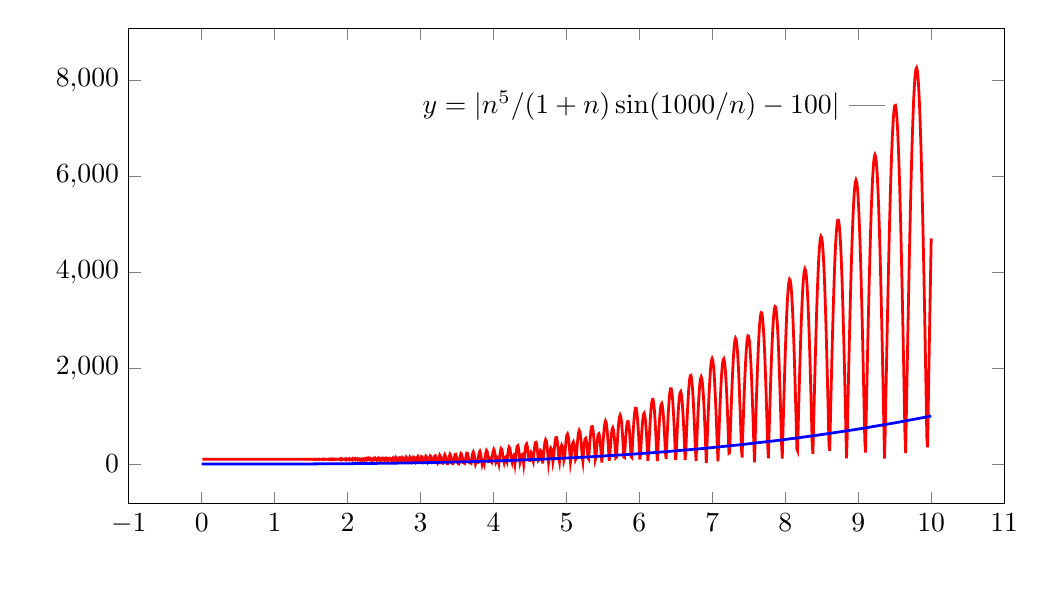
\begin{tikzpicture}[line width=1]
\begin{axis}[width=5in, height=3in,
             scatter/classes={a={mark=*,draw=black}},
             xlabel={\mbox{}},
             xlabel style={name=xlabel}, 
             ylabel={\mbox{}}, 
             legend style={
                at={(xlabel.south)},
                yshift=-1ex,
                anchor=north,
                legend cell align=left,
                },
        ]
]
\addplot[draw=red, line width=1] coordinates {(0.01,100.0)
(0.02,100.0)
(0.03,100.0)
(0.04,100.0)
(0.0501,100.0)
(0.0601,100.0)
(0.0701,100.0)
(0.0801,100.0)
(0.0901,100.0)
(0.1001,100.0)
(0.1101,100.0)
(0.1201,100.0)
(0.1301,100.0)
(0.1401,100.0)
(0.1502,100.0)
(0.1602,100.0001)
(0.1702,99.9999)
(0.1802,99.9999)
(0.1902,100.0002)
(0.2002,100.0)
(0.2102,99.9998)
(0.2202,100.0004)
(0.2302,99.9995)
(0.2402,99.9999)
(0.2503,100.0001)
(0.2603,100.0001)
(0.2703,100.0008)
(0.2803,100.0011)
(0.2903,99.9984)
(0.3003,100.0002)
(0.3103,100.0014)
(0.3203,100.0019)
(0.3303,100.0028)
(0.3403,100.0026)
(0.3504,99.9961)
(0.3604,100.0037)
(0.3704,100.005)
(0.3804,99.9969)
(0.3904,100.0059)
(0.4004,99.9995)
(0.4104,100.0079)
(0.4204,100.0035)
(0.4304,100.0103)
(0.4404,99.9909)
(0.4505,99.9886)
(0.4605,100.0111)
(0.4705,99.9848)
(0.4805,99.9827)
(0.4905,99.9978)
(0.5005,100.0011)
(0.5105,100.0229)
(0.5205,100.0251)
(0.5305,100.0014)
(0.5405,99.9884)
(0.5506,99.9837)
(0.5606,100.0169)
(0.5706,100.0142)
(0.5806,99.9695)
(0.5906,99.9956)
(0.6006,100.0022)
(0.6106,100.0424)
(0.6206,99.9807)
(0.6306,99.9565)
(0.6406,99.9723)
(0.6507,100.0447)
(0.6607,100.0435)
(0.6707,99.924)
(0.6807,100.0793)
(0.6907,99.9597)
(0.7007,99.9247)
(0.7107,100.0404)
(0.7207,100.0999)
(0.7307,100.1139)
(0.7407,100.0991)
(0.7508,100.0048)
(0.7608,99.861)
(0.7708,99.9885)
(0.7808,100.1372)
(0.7908,99.8277)
(0.8008,100.1828)
(0.8108,99.8129)
(0.8208,100.1231)
(0.8308,100.0811)
(0.8408,99.7759)
(0.8509,99.92)
(0.8609,100.1753)
(0.8709,100.2677)
(0.8809,100.2529)
(0.8909,100.2367)
(0.9009,100.2657)
(0.9109,100.3226)
(0.9209,100.3106)
(0.9309,100.083)
(0.9409,99.7005)
(0.951,99.6993)
(0.961,100.2872)
(0.971,100.2272)
(0.981,99.5422)
(0.991,100.2866)
(1.001,100.0133)
(1.011,99.7515)
(1.021,100.3803)
(1.031,99.5693)
(1.041,100.4085)
(1.0511,99.7145)
(1.0611,100.0163)
(1.0711,100.3797)
(1.0811,99.3044)
(1.0911,100.5463)
(1.1011,100.1992)
(1.1111,99.1996)
(1.1211,100.205)
(1.1311,100.8332)
(1.1411,99.8306)
(1.1512,99.0613)
(1.1612,99.6102)
(1.1712,100.6279)
(1.1812,101.0529)
(1.1912,100.6972)
(1.2012,99.9749)
(1.2112,99.316)
(1.2212,98.9084)
(1.2312,98.7374)
(1.2412,98.7051)
(1.2513,98.7135)
(1.2613,98.6972)
(1.2713,98.6291)
(1.2813,98.5218)
(1.2913,98.4333)
(1.3013,98.4725)
(1.3113,98.7831)
(1.3213,99.4779)
(1.3313,100.5081)
(1.3413,101.5244)
(1.3514,101.8936)
(1.3614,101.075)
(1.3714,99.3033)
(1.3814,97.9406)
(1.3914,98.5626)
(1.4014,100.9381)
(1.4114,102.315)
(1.4214,100.4658)
(1.4314,97.7263)
(1.4414,98.6852)
(1.4515,102.1477)
(1.4615,101.5752)
(1.4715,97.6395)
(1.4815,98.7688)
(1.4915,102.8627)
(1.5015,100.0538)
(1.5115,96.9846)
(1.5215,101.9416)
(1.5315,101.6252)
(1.5415,96.5773)
(1.5516,101.6573)
(1.5616,101.7388)
(1.5716,96.3051)
(1.5816,102.7984)
(1.5916,100.0656)
(1.6016,97.0887)
(1.6116,104.1607)
(1.6216,96.6112)
(1.6316,101.1842)
(1.6416,101.4311)
(1.6517,96.4487)
(1.6617,104.6718)
(1.6717,95.2906)
(1.6817,103.8715)
(1.6917,97.5104)
(1.7017,100.8896)
(1.7117,100.6794)
(1.7217,97.9346)
(1.7317,103.2022)
(1.7417,95.9153)
(1.7518,104.7427)
(1.7618,94.7808)
(1.7718,105.5553)
(1.7818,94.2201)
(1.7918,105.9045)
(1.8018,94.0809)
(1.8118,105.792)
(1.8218,94.5292)
(1.8318,104.8871)
(1.8418,96.0333)
(1.8519,102.6468)
(1.8619,99.0985)
(1.8719,98.7737)
(1.8819,103.5905)
(1.8919,94.0828)
(1.9019,107.8044)
(1.9119,91.2332)
(1.9219,108.3379)
(1.9319,93.7686)
(1.9419,102.5287)
(1.952,102.1706)
(1.962,93.268)
(1.972,109.6948)
(1.982,90.2638)
(1.992,106.3004)
(2.002,99.8583)
(2.012,93.4337)
(2.022,110.8471)
(2.032,89.7559)
(2.042,104.3574)
(2.0521,104.3135)
(2.0621,88.9055)
(2.0721,111.573)
(2.0821,95.3475)
(2.0921,94.1491)
(2.1021,112.8617)
(2.1121,89.2482)
(2.1221,100.1721)
(2.1321,111.165)
(2.1421,86.2686)
(2.1522,104.3922)
(2.1622,109.4646)
(2.1722,84.875)
(2.1822,106.2788)
(2.1922,109.388)
(2.2022,83.9634)
(2.2122,105.7045)
(2.2222,111.4917)
(2.2322,83.6447)
(2.2422,102.1623)
(2.2523,115.3265)
(2.2623,85.449)
(2.2723,95.1491)
(2.2823,118.7818)
(2.2923,91.8666)
(2.3023,85.839)
(2.3123,117.5281)
(2.3223,104.1439)
(2.3323,79.3426)
(2.3423,106.9063)
(2.3524,117.9793)
(2.3624,84.1523)
(2.3724,88.4371)
(2.3824,121.3509)
(2.3924,103.6763)
(2.4024,76.4811)
(2.4124,103.9897)
(2.4224,123.2152)
(2.4324,89.4886)
(2.4424,78.4954)
(2.4525,115.5909)
(2.4625,119.3337)
(2.4725,80.691)
(2.4825,82.5854)
(2.4925,121.8984)
(2.5025,116.2298)
(2.5125,76.4175)
(2.5225,83.9191)
(2.5325,124.476)
(2.5425,117.1332)
(2.5526,75.4692)
(2.5626,80.5715)
(2.5726,123.5181)
(2.5826,122.8565)
(2.5926,78.9562)
(2.6026,72.9149)
(2.6126,116.6155)
(2.6226,131.4681)
(2.6326,90.2189)
(2.6426,65.0309)
(2.6527,100.3591)
(2.6627,136.1652)
(2.6727,111.2488)
(2.6827,66.5771)
(2.6927,76.269)
(2.7027,125.3258)
(2.7127,134.6763)
(2.7227,88.6249)
(2.7327,59.2491)
(2.7427,92.829)
(2.7528,138.4801)
(2.7628,126.6767)
(2.7728,74.2894)
(2.7828,58.7105)
(2.7928,103.4479)
(2.8028,144.4373)
(2.8128,122.7875)
(2.8228,68.2253)
(2.8328,56.6493)
(2.8428,104.7187)
(2.8529,147.6561)
(2.8629,127.4459)
(2.8729,70.1016)
(2.8829,50.5877)
(2.8929,94.8274)
(2.9029,146.8884)
(2.9129,140.805)
(2.9229,83.3933)
(2.9329,45.056)
(2.9429,72.9663)
(2.953,134.2823)
(2.963,156.2209)
(2.973,112.3702)
(2.983,52.9834)
(2.993,46.2618)
(3.003,100.5382)
(3.013,155.5643)
(3.023,150.2114)
(3.033,89.593)
(3.043,38.7764)
(3.0531,52.357)
(3.0631,116.7428)
(3.0731,165.158)
(3.0831,147.3267)
(3.0931,80.6805)
(3.1031,31.9667)
(3.1131,50.034)
(3.1231,117.8389)
(3.1331,169.8365)
(3.1431,155.726)
(3.1532,88.1914)
(3.1632,30.2144)
(3.1732,35.861)
(3.1832,100.6502)
(3.1932,166.3266)
(3.2032,173.8673)
(3.2132,115.9348)
(3.2232,42.7)
(3.2332,17.5855)
(3.2432,62.665)
(3.2533,140.4329)
(3.2633,185.9931)
(3.2733,161.2194)
(3.2833,85.6927)
(3.2933,20.1203)
(3.3033,17.1679)
(3.3133,79.8156)
(3.3233,159.6335)
(3.3333,194.9436)
(3.3433,158.2441)
(3.3534,76.6251)
(3.3634,10.7952)
(3.3734,9.6847)
(3.3834,74.739)
(3.3934,159.4614)
(3.4034,203.329)
(3.4134,174.8611)
(3.4234,93.3229)
(3.4334,14.7371)
(3.4434,6.9867)
(3.4535,43.415)
(3.4635,132.8045)
(3.4735,202.2344)
(3.4835,205.9565)
(3.4935,140.9551)
(3.5035,48.3478)
(3.5135,13.2874)
(3.5235,4.9412)
(3.5335,68.8218)
(3.5435,163.2172)
(3.5536,220.9944)
(3.5636,207.0542)
(3.5736,129.0734)
(3.5836,32.4443)
(3.5936,26.6619)
(3.6036,13.8306)
(3.6136,64.2283)
(3.6236,163.9863)
(3.6336,229.8827)
(3.6436,225.1968)
(3.6537,151.9038)
(3.6637,49.1185)
(3.6737,28.3288)
(3.6837,39.1637)
(3.6937,22.8438)
(3.7037,126.0836)
(3.7137,217.8269)
(3.7237,251.3134)
(3.7337,209.2176)
(3.7437,111.9136)
(3.7538,6.9539)
(3.7638,54.4841)
(3.7738,42.3722)
(3.7838,38.071)
(3.7938,149.2919)
(3.8038,239.4049)
(3.8138,266.4424)
(3.8238,217.5042)
(3.8338,114.2599)
(3.8438,2.7648)
(3.8539,67.3644)
(3.8639,64.8811)
(3.8739,9.6737)
(3.8839,124.6003)
(3.8939,230.9981)
(3.9039,283.706)
(3.9139,260.2091)
(3.9239,169.7138)
(3.9339,48.9672)
(3.9439,53.0556)
(3.954,95.06)
(3.964,59.8343)
(3.974,39.239)
(3.984,163.8028)
(3.994,265.7136)
(4.004,305.6579)
(4.014,268.0019)
(4.024,166.3913)
(4.034,38.2997)
(4.044,69.1136)
(4.0541,116.3856)
(4.0641,85.9629)
(4.0741,11.7625)
(4.0841,142.4905)
(4.0941,260.3889)
(4.1041,324.2276)
(4.1141,311.5746)
(4.1241,226.2484)
(4.1341,96.7038)
(4.1441,33.8274)
(4.1542,121.9046)
(4.1642,138.2051)
(4.1742,76.9314)
(4.1842,42.5969)
(4.1942,182.4395)
(4.2042,298.3106)
(4.2142,353.5915)
(4.2242,330.6551)
(4.2342,236.0829)
(4.2442,98.3609)
(4.2543,41.0217)
(4.2643,140.194)
(4.2743,169.3743)
(4.2843,119.5117)
(4.2943,4.685)
(4.3043,142.2508)
(4.3143,279.3187)
(4.3243,367.4679)
(4.3343,381.547)
(4.3443,317.1653)
(4.3544,191.6625)
(4.3644,39.0954)
(4.3744,99.2193)
(4.3844,185.9235)
(4.3944,197.5483)
(4.4044,130.5626)
(4.4144,2.0652)
(4.4244,154.9025)
(4.4344,300.0578)
(4.4444,396.2519)
(4.4545,418.8378)
(4.4645,361.7112)
(4.4745,238.6124)
(4.4845,79.5078)
(4.4945,76.923)
(4.5045,192.7602)
(4.5145,239.9437)
(4.5245,206.8396)
(4.5345,100.7975)
(4.5445,53.7886)
(4.5546,221.3355)
(4.5646,363.3827)
(4.5746,447.3955)
(4.5846,454.0514)
(4.5946,381.4195)
(4.6046,245.1909)
(4.6146,75.0207)
(4.6246,92.1093)
(4.6346,219.9834)
(4.6446,280.9209)
(4.6547,261.5729)
(4.6647,165.5791)
(4.6747,12.6129)
(4.6847,165.8837)
(4.6947,333.3053)
(4.7047,455.4141)
(4.7147,507.2435)
(4.7247,478.0062)
(4.7347,373.0822)
(4.7447,212.7758)
(4.7548,28.1733)
(4.7648,145.0128)
(4.7748,273.3724)
(4.7848,332.1524)
(4.7948,309.8484)
(4.8048,210.2191)
(4.8148,51.4161)
(4.8248,137.5289)
(4.8348,322.1453)
(4.8448,468.85)
(4.8549,550.9924)
(4.8649,553.5444)
(4.8749,475.6387)
(4.8849,330.5656)
(4.8949,143.2986)
(4.9049,53.9576)
(4.9149,227.3763)
(4.9249,347.2903)
(4.9349,393.1595)
(4.9449,356.9155)
(4.955,244.1682)
(4.965,73.1315)
(4.975,128.4941)
(4.985,328.1222)
(4.995,493.5829)
(5.005,598.2596)
(5.015,625.2496)
(5.025,569.9188)
(5.035,440.4934)
(5.045,256.6479)
(5.0551,46.3603)
(5.0651,158.4425)
(5.0751,326.7551)
(5.0851,433.1376)
(5.0951,461.4444)
(5.1051,407.1111)
(5.1151,277.7012)
(5.1251,91.677)
(5.1351,124.3808)
(5.1451,339.6664)
(5.1552,523.5725)
(5.1652,650.0059)
(5.1752,700.992)
(5.1852,669.0871)
(5.1952,558.2938)
(5.2052,383.3936)
(5.2152,167.8279)
(5.2252,59.5512)
(5.2352,268.3947)
(5.2452,430.9003)
(5.2553,525.4468)
(5.2653,539.3571)
(5.2753,470.4494)
(5.2853,327.2099)
(5.2953,127.5982)
(5.3053,103.3283)
(5.3153,336.642)
(5.3253,543.1995)
(5.3353,697.2584)
(5.3453,779.6115)
(5.3554,779.8667)
(5.3654,697.6176)
(5.3754,542.3905)
(5.3854,332.4048)
(5.3954,92.3232)
(5.4054,149.718)
(5.4154,365.4332)
(5.4254,529.6712)
(5.4354,623.2809)
(5.4454,635.2404)
(5.4555,563.8268)
(5.4655,416.7162)
(5.4755,210.0311)
(5.4855,33.536)
(5.4955,287.2897)
(5.5055,523.495)
(5.5155,716.4016)
(5.5255,845.003)
(5.5355,895.2392)
(5.5455,861.4236)
(5.5556,746.7601)
(5.5656,562.9189)
(5.5756,328.7378)
(5.5856,68.2046)
(5.5956,192.0561)
(5.6056,425.5216)
(5.6156,608.4537)
(5.6256,722.2564)
(5.6356,755.2801)
(5.6456,703.9079)
(5.6557,572.8322)
(5.6657,374.516)
(5.6757,127.9074)
(5.6857,143.4476)
(5.6957,413.702)
(5.7057,657.1849)
(5.7157,850.8205)
(5.7257,976.2641)
(5.7357,1021.5625)
(5.7457,982.1965)
(5.7558,861.4232)
(5.7658,669.9049)
(5.7758,424.6732)
(5.7858,147.5376)
(5.7958,136.9059)
(5.8058,403.4815)
(5.8158,628.6542)
(5.8258,792.5717)
(5.8358,880.7525)
(5.8458,885.2833)
(5.8559,805.4341)
(5.8659,647.6526)
(5.8759,424.9509)
(5.8859,155.7521)
(5.8959,137.6967)
(5.9059,431.2014)
(5.9159,700.6293)
(5.9259,923.8786)
(5.9359,1082.6529)
(5.9459,1163.8995)
(5.956,1160.805)
(5.966,1073.2786)
(5.976,907.8968)
(5.986,677.3248)
(5.996,399.2733)
(6.006,95.0801)
(6.016,211.9644)
(6.026,498.4143)
(6.036,742.4492)
(6.046,925.5042)
(6.0561,1033.6299)
(6.0661,1058.4883)
(6.0761,997.9168)
(6.0861,856.0307)
(6.0961,642.8651)
(6.1061,373.5935)
(6.1161,67.3878)
(6.1261,253.9891)
(6.1361,567.7541)
(6.1461,851.7221)
(6.1562,1085.8563)
(6.1662,1253.6457)
(6.1762,1343.2166)
(6.1862,1348.1071)
(6.1962,1267.6603)
(6.2062,1107.0161)
(6.2162,876.7122)
(6.2262,591.9288)
(6.2362,271.4353)
(6.2462,63.6846)
(6.2563,391.4404)
(6.2663,690.3803)
(6.2763,940.9798)
(6.2863,1126.8847)
(6.2963,1235.931)
(6.3063,1260.883)
(6.3163,1199.8477)
(6.3263,1056.3463)
(6.3363,839.0459)
(6.3463,561.1756)
(6.3564,239.6689)
(6.3664,105.9074)
(6.3764,454.5703)
(6.3864,785.2036)
(6.3964,1077.8314)
(6.4064,1314.8029)
(6.4164,1481.822)
(6.4264,1568.7624)
(6.4364,1570.2264)
(6.4464,1485.8181)
(6.4565,1320.1229)
(6.4665,1082.3998)
(6.4765,786.0103)
(6.4865,447.6213)
(6.4965,86.2338)
(6.5065,277.9063)
(6.5165,624.4512)
(6.5265,934.0821)
(6.5365,1189.5674)
(6.5465,1376.6908)
(6.5566,1485.0002)
(6.5666,1508.3429)
(6.5766,1445.1595)
(6.5866,1298.5285)
(6.5966,1075.9625)
(6.6066,788.9728)
(6.6166,452.4296)
(6.6266,83.756)
(6.6366,297.9995)
(6.6466,673.1604)
(6.6567,1022.4384)
(6.6667,1327.9144)
(6.6767,1573.9362)
(6.6867,1747.8884)
(6.6967,1840.7998)
(6.7067,1847.7589)
(6.7167,1768.1241)
(6.7267,1605.5182)
(6.7367,1367.616)
(6.7467,1065.7367)
(6.7568,714.2655)
(6.7668,329.9361)
(6.7768,68.9885)
(6.7868,463.5974)
(6.7968,835.2301)
(6.8068,1166.3514)
(6.8168,1441.3606)
(6.8268,1647.3)
(6.8368,1774.4306)
(6.8468,1816.6526)
(6.8569,1771.7533)
(6.8669,1641.4757)
(6.8769,1431.407)
(6.8869,1150.6966)
(6.8969,811.619)
(6.9069,429.0041)
(6.9169,19.5631)
(6.9269,398.8589)
(6.9369,808.0693)
(6.9469,1190.3187)
(6.957,1529.0612)
(6.967,1809.653)
(6.977,2019.9598)
(6.987,2150.8501)
(6.997,2196.5552)
(7.007,2154.8827)
(7.017,2027.2793)
(7.027,1818.741)
(7.037,1537.5795)
(7.047,1195.0553)
(7.0571,804.8959)
(7.0671,382.7213)
(7.0771,54.5992)
(7.0871,489.6318)
(7.0971,905.0753)
(7.1071,1284.444)
(7.1171,1612.7094)
(7.1271,1876.8756)
(7.1371,2066.4685)
(7.1471,2173.9204)
(7.1572,2194.8377)
(7.1672,2128.1438)
(7.1772,1976.0935)
(7.1872,1744.1613)
(7.1972,1440.8107)
(7.2072,1077.1534)
(7.2172,666.516)
(7.2272,223.9298)
(7.2372,234.4355)
(7.2472,691.8714)
(7.2573,1131.743)
(7.2673,1538.0891)
(7.2773,1896.1916)
(7.2873,2193.0916)
(7.2973,2418.0368)
(7.3073,2562.8448)
(7.3173,2622.1705)
(7.3273,2593.6712)
(7.3373,2478.0649)
(7.3473,2279.0816)
(7.3574,2003.3115)
(7.3674,1659.9574)
(7.3774,1260.5008)
(7.3874,818.296)
(7.3974,348.1055)
(7.4074,134.4053)
(7.4174,613.197)
(7.4274,1072.3903)
(7.4374,1496.789)
(7.4474,1872.3719)
(7.4575,2186.7417)
(7.4675,2429.5146)
(7.4775,2592.6398)
(7.4875,2670.6399)
(7.4975,2660.7665)
(7.5075,2563.0662)
(7.5175,2380.3582)
(7.5275,2118.1249)
(7.5375,1784.3197)
(7.5475,1389.1018)
(7.5576,944.5052)
(7.5676,464.0542)
(7.5776,37.6612)
(7.5876,545.4374)
(7.5976,1043.9219)
(7.6076,1518.0771)
(7.6176,1953.6277)
(7.6276,2337.4809)
(7.6376,2658.1053)
(7.6476,2905.8591)
(7.6577,3073.2591)
(7.6677,3155.1827)
(7.6777,3148.999)
(7.6877,3054.6262)
(7.6977,2874.5152)
(7.7077,2613.5606)
(7.7177,2278.9431)
(7.7277,1879.9103)
(7.7377,1427.5004)
(7.7477,934.2203)
(7.7578,413.6868)
(7.7678,119.7591)
(7.7778,651.4529)
(7.7878,1166.8108)
(7.7978,1651.7267)
(7.8078,2092.9521)
(7.8178,2478.4471)
(7.8278,2797.6951)
(7.8378,3041.9724)
(7.8478,3204.5675)
(7.8579,3280.9439)
(7.8679,3268.8431)
(7.8779,3168.328)
(7.8879,2981.7636)
(7.8979,2713.7394)
(7.9079,2370.9351)
(7.9179,1961.9334)
(7.9279,1496.9877)
(7.9379,987.7496)
(7.9479,446.9637)
(7.958,111.86)
(7.968,674.79)
(7.978,1227.8233)
(7.988,1757.2324)
(7.998,2249.9018)
(8.008,2693.6456)
(8.018,3077.4974)
(8.028,3391.9688)
(8.038,3629.2672)
(8.048,3783.4716)
(8.0581,3850.6607)
(8.0681,3828.9918)
(8.0781,3718.7302)
(8.0881,3522.2273)
(8.0981,3243.8511)
(8.1081,2889.8701)
(8.1181,2468.2937)
(8.1281,1988.6756)
(8.1381,1461.8826)
(8.1481,899.8372)
(8.1582,315.2384)
(8.1682,278.7313)
(8.1782,868.7064)
(8.1882,1441.4397)
(8.1982,1984.0972)
(8.2082,2484.5402)
(8.2182,2931.5888)
(8.2282,3315.2613)
(8.2382,3626.9842)
(8.2482,3859.7693)
(8.2583,4008.3543)
(8.2683,4069.3038)
(8.2783,4041.071)
(8.2883,3924.0174)
(8.2983,3720.3917)
(8.3083,3434.2696)
(8.3183,3071.4548)
(8.3283,2639.3457)
(8.3383,2146.77)
(8.3483,1603.7917)
(8.3584,1021.4945)
(8.3684,411.7469)
(8.3784,213.046)
(8.3884,840.199)
(8.3984,1457.0054)
(8.4084,2050.9941)
(8.4184,2610.1779)
(8.4284,3123.2898)
(8.4384,3580.0025)
(8.4484,3971.1259)
(8.4585,4288.7808)
(8.4685,4526.5441)
(8.4785,4679.5647)
(8.4885,4744.6465)
(8.4985,4720.2997)
(8.5085,4606.7571)
(8.5185,4405.9584)
(8.5285,4121.502)
(8.5385,3758.5647)
(8.5485,3323.7943)
(8.5586,2825.1741)
(8.5686,2271.8646)
(8.5786,1674.0256)
(8.5886,1042.6205)
(8.5986,389.2092)
(8.6086,274.2684)
(8.6186,935.713)
(8.6286,1583.0872)
(8.6386,2204.6326)
(8.6486,2789.0806)
(8.6587,3325.8505)
(8.6687,3805.2345)
(8.6787,4218.5638)
(8.6887,4558.3557)
(8.6987,4818.437)
(8.7087,4994.0438)
(8.7187,5081.8954)
(8.7287,5080.2412)
(8.7387,4988.8809)
(8.7487,4809.1581)
(8.7588,4543.9264)
(8.7688,4197.4917)
(8.7788,3775.5288)
(8.7888,3284.9769)
(8.7988,2733.9144)
(8.8088,2131.4163)
(8.8188,1487.3963)
(8.8288,812.4369)
(8.8388,117.6102)
(8.8488,585.7074)
(8.8589,1286.0235)
(8.8689,1971.9175)
(8.8789,2632.2255)
(8.8889,3256.2192)
(8.8989,3833.7751)
(8.9089,4355.5328)
(8.9189,4813.0394)
(8.9289,5198.8771)
(8.9389,5506.7746)
(8.9489,5731.6974)
(8.959,5869.9189)
(8.969,5919.0703)
(8.979,5878.1682)
(8.989,5747.6213)
(8.999,5529.2146)
(9.009,5226.074)
(9.019,4842.6093)
(9.029,4384.4398)
(9.039,3858.3012)
(9.049,3271.9374)
(9.0591,2633.9782)
(9.0691,1953.8049)
(9.0791,1241.4065)
(9.0891,507.228)
(9.0991,237.9858)
(9.1091,983.3496)
(9.1191,1717.9973)
(9.1291,2431.2395)
(9.1391,3112.7168)
(9.1491,3752.5469)
(9.1592,4341.4631)
(9.1692,4870.9425)
(9.1792,5333.3222)
(9.1892,5721.9027)
(9.1992,6031.0355)
(9.2092,6256.1964)
(9.2192,6394.0408)
(9.2292,6442.4435)
(9.2392,6400.5198)
(9.2492,6268.6306)
(9.2593,6048.3689)
(9.2693,5742.531)
(9.2793,5355.071)
(9.2893,4891.0393)
(9.2993,4356.5085)
(9.3093,3758.4852)
(9.3193,3104.8108)
(9.3293,2404.0514)
(9.3393,1665.3806)
(9.3493,898.4541)
(9.3594,113.2802)
(9.3694,679.9134)
(9.3794,1470.8142)
(9.3894,2249.159)
(9.3994,3004.8663)
(9.4094,3728.1648)
(9.4194,4409.7164)
(9.4294,5040.733)
(9.4394,5613.0843)
(9.4494,6119.3966)
(9.4595,6553.1412)
(9.4695,6908.7112)
(9.4795,7181.4852)
(9.4895,7367.8793)
(9.4995,7465.3852)
(9.5095,7472.594)
(9.5195,7389.2074)
(9.5295,7216.034)
(9.5395,6954.9736)
(9.5495,6608.9865)
(9.5596,6182.0521)
(9.5696,5679.1147)
(9.5796,5106.0185)
(9.5896,4469.4322)
(9.5996,3776.7655)
(9.6096,3036.0765)
(9.6196,2255.9732)
(9.6296,1445.5093)
(9.6396,614.0757)
(9.6496,228.7105)
(9.6597,1073.1189)
(9.6697,1909.4183)
(9.6797,2727.9888)
(9.6897,3519.4309)
(9.6997,4274.6713)
(9.7097,4985.0636)
(9.7197,5642.4839)
(9.7297,6239.4183)
(9.7397,6769.0442)
(9.7497,7225.3016)
(9.7598,7602.9564)
(9.7698,7897.6532)
(9.7798,8105.9578)
(9.7898,8225.3899)
(9.7998,8254.4442)
(9.8098,8192.6014)
(9.8198,8040.3273)
(9.8298,7799.0629)
(9.8398,7471.2023)
(9.8498,7060.0619)
(9.8599,6569.8398)
(9.8699,6005.5653)
(9.8799,5373.0417)
(9.8899,4678.78)
(9.8999,3929.9268)
(9.9099,3134.1856)
(9.9199,2299.7338)
(9.9299,1435.1346)
(9.9399,549.2471)
(9.9499,348.8674)
(9.96,1250.0385)
(9.97,2145.0815)
(9.98,3024.8905)
(9.99,3880.5299)
(10.0,4703.324)
(10.0,4703.324)};\node[pin=left:{$y=|n^5/(1 + n)   \sin(1000/n) - 100|$}] at (axis cs:9.5,7467.8971870303885) {};\addplot[draw=blue, line width=1] coordinates {(0.0,0.0)
(0.5263,0.1458)
(1.0526,1.1664)
(1.5789,3.9364)
(2.1053,9.3308)
(2.6316,18.2242)
(3.1579,31.4915)
(3.6842,50.0073)
(4.2105,74.6464)
(4.7368,106.2837)
(5.2632,145.7938)
(5.7895,194.0516)
(6.3158,251.9318)
(6.8421,320.3091)
(7.3684,400.0583)
(7.8947,492.0542)
(8.4211,597.1716)
(8.9474,716.2852)
(9.4737,850.2697)
(10.0,1000.0)};
\end{axis}\end{tikzpicture}\end{center}

OK ... at least I can see $n^3$ bending up a little. 
But it's still not high enough to bound $f(n)$.

% 32 not used

With $g(n) = n^4$:
%-*-latex-*-

\begin{center}
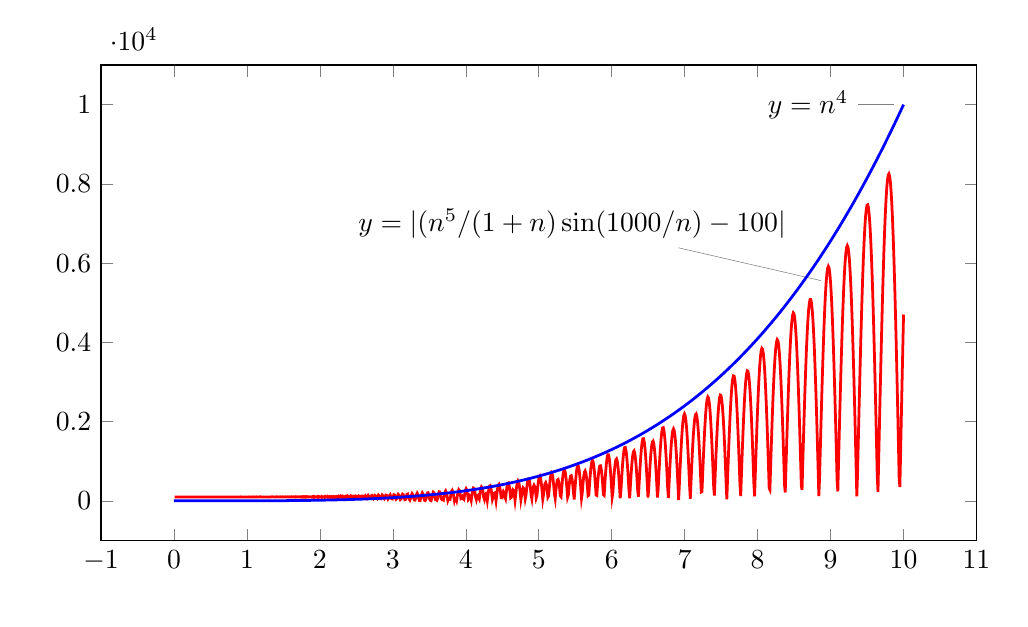
\begin{tikzpicture}[line width=1]
\begin{axis}[width=5in, height=3in,
             scatter/classes={a={mark=*,draw=black}},
             xlabel={\mbox{}},
             xlabel style={name=xlabel}, 
             ylabel={\mbox{}}, 
             legend style={
                at={(xlabel.south)},
                yshift=-1ex,
                anchor=north,
                legend cell align=left,
                },
        ]
]
\addplot[draw=red, line width=1] coordinates {(0.01,100.0)
(0.02,100.0)
(0.03,100.0)
(0.04,100.0)
(0.0501,100.0)
(0.0601,100.0)
(0.0701,100.0)
(0.0801,100.0)
(0.0901,100.0)
(0.1001,100.0)
(0.1101,100.0)
(0.1201,100.0)
(0.1301,100.0)
(0.1401,100.0)
(0.1502,100.0)
(0.1602,100.0001)
(0.1702,99.9999)
(0.1802,99.9999)
(0.1902,100.0002)
(0.2002,100.0)
(0.2102,99.9998)
(0.2202,100.0004)
(0.2302,99.9995)
(0.2402,99.9999)
(0.2503,100.0001)
(0.2603,100.0001)
(0.2703,100.0008)
(0.2803,100.0011)
(0.2903,99.9984)
(0.3003,100.0002)
(0.3103,100.0014)
(0.3203,100.0019)
(0.3303,100.0028)
(0.3403,100.0026)
(0.3504,99.9961)
(0.3604,100.0037)
(0.3704,100.005)
(0.3804,99.9969)
(0.3904,100.0059)
(0.4004,99.9995)
(0.4104,100.0079)
(0.4204,100.0035)
(0.4304,100.0103)
(0.4404,99.9909)
(0.4505,99.9886)
(0.4605,100.0111)
(0.4705,99.9848)
(0.4805,99.9827)
(0.4905,99.9978)
(0.5005,100.0011)
(0.5105,100.0229)
(0.5205,100.0251)
(0.5305,100.0014)
(0.5405,99.9884)
(0.5506,99.9837)
(0.5606,100.0169)
(0.5706,100.0142)
(0.5806,99.9695)
(0.5906,99.9956)
(0.6006,100.0022)
(0.6106,100.0424)
(0.6206,99.9807)
(0.6306,99.9565)
(0.6406,99.9723)
(0.6507,100.0447)
(0.6607,100.0435)
(0.6707,99.924)
(0.6807,100.0793)
(0.6907,99.9597)
(0.7007,99.9247)
(0.7107,100.0404)
(0.7207,100.0999)
(0.7307,100.1139)
(0.7407,100.0991)
(0.7508,100.0048)
(0.7608,99.861)
(0.7708,99.9885)
(0.7808,100.1372)
(0.7908,99.8277)
(0.8008,100.1828)
(0.8108,99.8129)
(0.8208,100.1231)
(0.8308,100.0811)
(0.8408,99.7759)
(0.8509,99.92)
(0.8609,100.1753)
(0.8709,100.2677)
(0.8809,100.2529)
(0.8909,100.2367)
(0.9009,100.2657)
(0.9109,100.3226)
(0.9209,100.3106)
(0.9309,100.083)
(0.9409,99.7005)
(0.951,99.6993)
(0.961,100.2872)
(0.971,100.2272)
(0.981,99.5422)
(0.991,100.2866)
(1.001,100.0133)
(1.011,99.7515)
(1.021,100.3803)
(1.031,99.5693)
(1.041,100.4085)
(1.0511,99.7145)
(1.0611,100.0163)
(1.0711,100.3797)
(1.0811,99.3044)
(1.0911,100.5463)
(1.1011,100.1992)
(1.1111,99.1996)
(1.1211,100.205)
(1.1311,100.8332)
(1.1411,99.8306)
(1.1512,99.0613)
(1.1612,99.6102)
(1.1712,100.6279)
(1.1812,101.0529)
(1.1912,100.6972)
(1.2012,99.9749)
(1.2112,99.316)
(1.2212,98.9084)
(1.2312,98.7374)
(1.2412,98.7051)
(1.2513,98.7135)
(1.2613,98.6972)
(1.2713,98.6291)
(1.2813,98.5218)
(1.2913,98.4333)
(1.3013,98.4725)
(1.3113,98.7831)
(1.3213,99.4779)
(1.3313,100.5081)
(1.3413,101.5244)
(1.3514,101.8936)
(1.3614,101.075)
(1.3714,99.3033)
(1.3814,97.9406)
(1.3914,98.5626)
(1.4014,100.9381)
(1.4114,102.315)
(1.4214,100.4658)
(1.4314,97.7263)
(1.4414,98.6852)
(1.4515,102.1477)
(1.4615,101.5752)
(1.4715,97.6395)
(1.4815,98.7688)
(1.4915,102.8627)
(1.5015,100.0538)
(1.5115,96.9846)
(1.5215,101.9416)
(1.5315,101.6252)
(1.5415,96.5773)
(1.5516,101.6573)
(1.5616,101.7388)
(1.5716,96.3051)
(1.5816,102.7984)
(1.5916,100.0656)
(1.6016,97.0887)
(1.6116,104.1607)
(1.6216,96.6112)
(1.6316,101.1842)
(1.6416,101.4311)
(1.6517,96.4487)
(1.6617,104.6718)
(1.6717,95.2906)
(1.6817,103.8715)
(1.6917,97.5104)
(1.7017,100.8896)
(1.7117,100.6794)
(1.7217,97.9346)
(1.7317,103.2022)
(1.7417,95.9153)
(1.7518,104.7427)
(1.7618,94.7808)
(1.7718,105.5553)
(1.7818,94.2201)
(1.7918,105.9045)
(1.8018,94.0809)
(1.8118,105.792)
(1.8218,94.5292)
(1.8318,104.8871)
(1.8418,96.0333)
(1.8519,102.6468)
(1.8619,99.0985)
(1.8719,98.7737)
(1.8819,103.5905)
(1.8919,94.0828)
(1.9019,107.8044)
(1.9119,91.2332)
(1.9219,108.3379)
(1.9319,93.7686)
(1.9419,102.5287)
(1.952,102.1706)
(1.962,93.268)
(1.972,109.6948)
(1.982,90.2638)
(1.992,106.3004)
(2.002,99.8583)
(2.012,93.4337)
(2.022,110.8471)
(2.032,89.7559)
(2.042,104.3574)
(2.0521,104.3135)
(2.0621,88.9055)
(2.0721,111.573)
(2.0821,95.3475)
(2.0921,94.1491)
(2.1021,112.8617)
(2.1121,89.2482)
(2.1221,100.1721)
(2.1321,111.165)
(2.1421,86.2686)
(2.1522,104.3922)
(2.1622,109.4646)
(2.1722,84.875)
(2.1822,106.2788)
(2.1922,109.388)
(2.2022,83.9634)
(2.2122,105.7045)
(2.2222,111.4917)
(2.2322,83.6447)
(2.2422,102.1623)
(2.2523,115.3265)
(2.2623,85.449)
(2.2723,95.1491)
(2.2823,118.7818)
(2.2923,91.8666)
(2.3023,85.839)
(2.3123,117.5281)
(2.3223,104.1439)
(2.3323,79.3426)
(2.3423,106.9063)
(2.3524,117.9793)
(2.3624,84.1523)
(2.3724,88.4371)
(2.3824,121.3509)
(2.3924,103.6763)
(2.4024,76.4811)
(2.4124,103.9897)
(2.4224,123.2152)
(2.4324,89.4886)
(2.4424,78.4954)
(2.4525,115.5909)
(2.4625,119.3337)
(2.4725,80.691)
(2.4825,82.5854)
(2.4925,121.8984)
(2.5025,116.2298)
(2.5125,76.4175)
(2.5225,83.9191)
(2.5325,124.476)
(2.5425,117.1332)
(2.5526,75.4692)
(2.5626,80.5715)
(2.5726,123.5181)
(2.5826,122.8565)
(2.5926,78.9562)
(2.6026,72.9149)
(2.6126,116.6155)
(2.6226,131.4681)
(2.6326,90.2189)
(2.6426,65.0309)
(2.6527,100.3591)
(2.6627,136.1652)
(2.6727,111.2488)
(2.6827,66.5771)
(2.6927,76.269)
(2.7027,125.3258)
(2.7127,134.6763)
(2.7227,88.6249)
(2.7327,59.2491)
(2.7427,92.829)
(2.7528,138.4801)
(2.7628,126.6767)
(2.7728,74.2894)
(2.7828,58.7105)
(2.7928,103.4479)
(2.8028,144.4373)
(2.8128,122.7875)
(2.8228,68.2253)
(2.8328,56.6493)
(2.8428,104.7187)
(2.8529,147.6561)
(2.8629,127.4459)
(2.8729,70.1016)
(2.8829,50.5877)
(2.8929,94.8274)
(2.9029,146.8884)
(2.9129,140.805)
(2.9229,83.3933)
(2.9329,45.056)
(2.9429,72.9663)
(2.953,134.2823)
(2.963,156.2209)
(2.973,112.3702)
(2.983,52.9834)
(2.993,46.2618)
(3.003,100.5382)
(3.013,155.5643)
(3.023,150.2114)
(3.033,89.593)
(3.043,38.7764)
(3.0531,52.357)
(3.0631,116.7428)
(3.0731,165.158)
(3.0831,147.3267)
(3.0931,80.6805)
(3.1031,31.9667)
(3.1131,50.034)
(3.1231,117.8389)
(3.1331,169.8365)
(3.1431,155.726)
(3.1532,88.1914)
(3.1632,30.2144)
(3.1732,35.861)
(3.1832,100.6502)
(3.1932,166.3266)
(3.2032,173.8673)
(3.2132,115.9348)
(3.2232,42.7)
(3.2332,17.5855)
(3.2432,62.665)
(3.2533,140.4329)
(3.2633,185.9931)
(3.2733,161.2194)
(3.2833,85.6927)
(3.2933,20.1203)
(3.3033,17.1679)
(3.3133,79.8156)
(3.3233,159.6335)
(3.3333,194.9436)
(3.3433,158.2441)
(3.3534,76.6251)
(3.3634,10.7952)
(3.3734,9.6847)
(3.3834,74.739)
(3.3934,159.4614)
(3.4034,203.329)
(3.4134,174.8611)
(3.4234,93.3229)
(3.4334,14.7371)
(3.4434,6.9867)
(3.4535,43.415)
(3.4635,132.8045)
(3.4735,202.2344)
(3.4835,205.9565)
(3.4935,140.9551)
(3.5035,48.3478)
(3.5135,13.2874)
(3.5235,4.9412)
(3.5335,68.8218)
(3.5435,163.2172)
(3.5536,220.9944)
(3.5636,207.0542)
(3.5736,129.0734)
(3.5836,32.4443)
(3.5936,26.6619)
(3.6036,13.8306)
(3.6136,64.2283)
(3.6236,163.9863)
(3.6336,229.8827)
(3.6436,225.1968)
(3.6537,151.9038)
(3.6637,49.1185)
(3.6737,28.3288)
(3.6837,39.1637)
(3.6937,22.8438)
(3.7037,126.0836)
(3.7137,217.8269)
(3.7237,251.3134)
(3.7337,209.2176)
(3.7437,111.9136)
(3.7538,6.9539)
(3.7638,54.4841)
(3.7738,42.3722)
(3.7838,38.071)
(3.7938,149.2919)
(3.8038,239.4049)
(3.8138,266.4424)
(3.8238,217.5042)
(3.8338,114.2599)
(3.8438,2.7648)
(3.8539,67.3644)
(3.8639,64.8811)
(3.8739,9.6737)
(3.8839,124.6003)
(3.8939,230.9981)
(3.9039,283.706)
(3.9139,260.2091)
(3.9239,169.7138)
(3.9339,48.9672)
(3.9439,53.0556)
(3.954,95.06)
(3.964,59.8343)
(3.974,39.239)
(3.984,163.8028)
(3.994,265.7136)
(4.004,305.6579)
(4.014,268.0019)
(4.024,166.3913)
(4.034,38.2997)
(4.044,69.1136)
(4.0541,116.3856)
(4.0641,85.9629)
(4.0741,11.7625)
(4.0841,142.4905)
(4.0941,260.3889)
(4.1041,324.2276)
(4.1141,311.5746)
(4.1241,226.2484)
(4.1341,96.7038)
(4.1441,33.8274)
(4.1542,121.9046)
(4.1642,138.2051)
(4.1742,76.9314)
(4.1842,42.5969)
(4.1942,182.4395)
(4.2042,298.3106)
(4.2142,353.5915)
(4.2242,330.6551)
(4.2342,236.0829)
(4.2442,98.3609)
(4.2543,41.0217)
(4.2643,140.194)
(4.2743,169.3743)
(4.2843,119.5117)
(4.2943,4.685)
(4.3043,142.2508)
(4.3143,279.3187)
(4.3243,367.4679)
(4.3343,381.547)
(4.3443,317.1653)
(4.3544,191.6625)
(4.3644,39.0954)
(4.3744,99.2193)
(4.3844,185.9235)
(4.3944,197.5483)
(4.4044,130.5626)
(4.4144,2.0652)
(4.4244,154.9025)
(4.4344,300.0578)
(4.4444,396.2519)
(4.4545,418.8378)
(4.4645,361.7112)
(4.4745,238.6124)
(4.4845,79.5078)
(4.4945,76.923)
(4.5045,192.7602)
(4.5145,239.9437)
(4.5245,206.8396)
(4.5345,100.7975)
(4.5445,53.7886)
(4.5546,221.3355)
(4.5646,363.3827)
(4.5746,447.3955)
(4.5846,454.0514)
(4.5946,381.4195)
(4.6046,245.1909)
(4.6146,75.0207)
(4.6246,92.1093)
(4.6346,219.9834)
(4.6446,280.9209)
(4.6547,261.5729)
(4.6647,165.5791)
(4.6747,12.6129)
(4.6847,165.8837)
(4.6947,333.3053)
(4.7047,455.4141)
(4.7147,507.2435)
(4.7247,478.0062)
(4.7347,373.0822)
(4.7447,212.7758)
(4.7548,28.1733)
(4.7648,145.0128)
(4.7748,273.3724)
(4.7848,332.1524)
(4.7948,309.8484)
(4.8048,210.2191)
(4.8148,51.4161)
(4.8248,137.5289)
(4.8348,322.1453)
(4.8448,468.85)
(4.8549,550.9924)
(4.8649,553.5444)
(4.8749,475.6387)
(4.8849,330.5656)
(4.8949,143.2986)
(4.9049,53.9576)
(4.9149,227.3763)
(4.9249,347.2903)
(4.9349,393.1595)
(4.9449,356.9155)
(4.955,244.1682)
(4.965,73.1315)
(4.975,128.4941)
(4.985,328.1222)
(4.995,493.5829)
(5.005,598.2596)
(5.015,625.2496)
(5.025,569.9188)
(5.035,440.4934)
(5.045,256.6479)
(5.0551,46.3603)
(5.0651,158.4425)
(5.0751,326.7551)
(5.0851,433.1376)
(5.0951,461.4444)
(5.1051,407.1111)
(5.1151,277.7012)
(5.1251,91.677)
(5.1351,124.3808)
(5.1451,339.6664)
(5.1552,523.5725)
(5.1652,650.0059)
(5.1752,700.992)
(5.1852,669.0871)
(5.1952,558.2938)
(5.2052,383.3936)
(5.2152,167.8279)
(5.2252,59.5512)
(5.2352,268.3947)
(5.2452,430.9003)
(5.2553,525.4468)
(5.2653,539.3571)
(5.2753,470.4494)
(5.2853,327.2099)
(5.2953,127.5982)
(5.3053,103.3283)
(5.3153,336.642)
(5.3253,543.1995)
(5.3353,697.2584)
(5.3453,779.6115)
(5.3554,779.8667)
(5.3654,697.6176)
(5.3754,542.3905)
(5.3854,332.4048)
(5.3954,92.3232)
(5.4054,149.718)
(5.4154,365.4332)
(5.4254,529.6712)
(5.4354,623.2809)
(5.4454,635.2404)
(5.4555,563.8268)
(5.4655,416.7162)
(5.4755,210.0311)
(5.4855,33.536)
(5.4955,287.2897)
(5.5055,523.495)
(5.5155,716.4016)
(5.5255,845.003)
(5.5355,895.2392)
(5.5455,861.4236)
(5.5556,746.7601)
(5.5656,562.9189)
(5.5756,328.7378)
(5.5856,68.2046)
(5.5956,192.0561)
(5.6056,425.5216)
(5.6156,608.4537)
(5.6256,722.2564)
(5.6356,755.2801)
(5.6456,703.9079)
(5.6557,572.8322)
(5.6657,374.516)
(5.6757,127.9074)
(5.6857,143.4476)
(5.6957,413.702)
(5.7057,657.1849)
(5.7157,850.8205)
(5.7257,976.2641)
(5.7357,1021.5625)
(5.7457,982.1965)
(5.7558,861.4232)
(5.7658,669.9049)
(5.7758,424.6732)
(5.7858,147.5376)
(5.7958,136.9059)
(5.8058,403.4815)
(5.8158,628.6542)
(5.8258,792.5717)
(5.8358,880.7525)
(5.8458,885.2833)
(5.8559,805.4341)
(5.8659,647.6526)
(5.8759,424.9509)
(5.8859,155.7521)
(5.8959,137.6967)
(5.9059,431.2014)
(5.9159,700.6293)
(5.9259,923.8786)
(5.9359,1082.6529)
(5.9459,1163.8995)
(5.956,1160.805)
(5.966,1073.2786)
(5.976,907.8968)
(5.986,677.3248)
(5.996,399.2733)
(6.006,95.0801)
(6.016,211.9644)
(6.026,498.4143)
(6.036,742.4492)
(6.046,925.5042)
(6.0561,1033.6299)
(6.0661,1058.4883)
(6.0761,997.9168)
(6.0861,856.0307)
(6.0961,642.8651)
(6.1061,373.5935)
(6.1161,67.3878)
(6.1261,253.9891)
(6.1361,567.7541)
(6.1461,851.7221)
(6.1562,1085.8563)
(6.1662,1253.6457)
(6.1762,1343.2166)
(6.1862,1348.1071)
(6.1962,1267.6603)
(6.2062,1107.0161)
(6.2162,876.7122)
(6.2262,591.9288)
(6.2362,271.4353)
(6.2462,63.6846)
(6.2563,391.4404)
(6.2663,690.3803)
(6.2763,940.9798)
(6.2863,1126.8847)
(6.2963,1235.931)
(6.3063,1260.883)
(6.3163,1199.8477)
(6.3263,1056.3463)
(6.3363,839.0459)
(6.3463,561.1756)
(6.3564,239.6689)
(6.3664,105.9074)
(6.3764,454.5703)
(6.3864,785.2036)
(6.3964,1077.8314)
(6.4064,1314.8029)
(6.4164,1481.822)
(6.4264,1568.7624)
(6.4364,1570.2264)
(6.4464,1485.8181)
(6.4565,1320.1229)
(6.4665,1082.3998)
(6.4765,786.0103)
(6.4865,447.6213)
(6.4965,86.2338)
(6.5065,277.9063)
(6.5165,624.4512)
(6.5265,934.0821)
(6.5365,1189.5674)
(6.5465,1376.6908)
(6.5566,1485.0002)
(6.5666,1508.3429)
(6.5766,1445.1595)
(6.5866,1298.5285)
(6.5966,1075.9625)
(6.6066,788.9728)
(6.6166,452.4296)
(6.6266,83.756)
(6.6366,297.9995)
(6.6466,673.1604)
(6.6567,1022.4384)
(6.6667,1327.9144)
(6.6767,1573.9362)
(6.6867,1747.8884)
(6.6967,1840.7998)
(6.7067,1847.7589)
(6.7167,1768.1241)
(6.7267,1605.5182)
(6.7367,1367.616)
(6.7467,1065.7367)
(6.7568,714.2655)
(6.7668,329.9361)
(6.7768,68.9885)
(6.7868,463.5974)
(6.7968,835.2301)
(6.8068,1166.3514)
(6.8168,1441.3606)
(6.8268,1647.3)
(6.8368,1774.4306)
(6.8468,1816.6526)
(6.8569,1771.7533)
(6.8669,1641.4757)
(6.8769,1431.407)
(6.8869,1150.6966)
(6.8969,811.619)
(6.9069,429.0041)
(6.9169,19.5631)
(6.9269,398.8589)
(6.9369,808.0693)
(6.9469,1190.3187)
(6.957,1529.0612)
(6.967,1809.653)
(6.977,2019.9598)
(6.987,2150.8501)
(6.997,2196.5552)
(7.007,2154.8827)
(7.017,2027.2793)
(7.027,1818.741)
(7.037,1537.5795)
(7.047,1195.0553)
(7.0571,804.8959)
(7.0671,382.7213)
(7.0771,54.5992)
(7.0871,489.6318)
(7.0971,905.0753)
(7.1071,1284.444)
(7.1171,1612.7094)
(7.1271,1876.8756)
(7.1371,2066.4685)
(7.1471,2173.9204)
(7.1572,2194.8377)
(7.1672,2128.1438)
(7.1772,1976.0935)
(7.1872,1744.1613)
(7.1972,1440.8107)
(7.2072,1077.1534)
(7.2172,666.516)
(7.2272,223.9298)
(7.2372,234.4355)
(7.2472,691.8714)
(7.2573,1131.743)
(7.2673,1538.0891)
(7.2773,1896.1916)
(7.2873,2193.0916)
(7.2973,2418.0368)
(7.3073,2562.8448)
(7.3173,2622.1705)
(7.3273,2593.6712)
(7.3373,2478.0649)
(7.3473,2279.0816)
(7.3574,2003.3115)
(7.3674,1659.9574)
(7.3774,1260.5008)
(7.3874,818.296)
(7.3974,348.1055)
(7.4074,134.4053)
(7.4174,613.197)
(7.4274,1072.3903)
(7.4374,1496.789)
(7.4474,1872.3719)
(7.4575,2186.7417)
(7.4675,2429.5146)
(7.4775,2592.6398)
(7.4875,2670.6399)
(7.4975,2660.7665)
(7.5075,2563.0662)
(7.5175,2380.3582)
(7.5275,2118.1249)
(7.5375,1784.3197)
(7.5475,1389.1018)
(7.5576,944.5052)
(7.5676,464.0542)
(7.5776,37.6612)
(7.5876,545.4374)
(7.5976,1043.9219)
(7.6076,1518.0771)
(7.6176,1953.6277)
(7.6276,2337.4809)
(7.6376,2658.1053)
(7.6476,2905.8591)
(7.6577,3073.2591)
(7.6677,3155.1827)
(7.6777,3148.999)
(7.6877,3054.6262)
(7.6977,2874.5152)
(7.7077,2613.5606)
(7.7177,2278.9431)
(7.7277,1879.9103)
(7.7377,1427.5004)
(7.7477,934.2203)
(7.7578,413.6868)
(7.7678,119.7591)
(7.7778,651.4529)
(7.7878,1166.8108)
(7.7978,1651.7267)
(7.8078,2092.9521)
(7.8178,2478.4471)
(7.8278,2797.6951)
(7.8378,3041.9724)
(7.8478,3204.5675)
(7.8579,3280.9439)
(7.8679,3268.8431)
(7.8779,3168.328)
(7.8879,2981.7636)
(7.8979,2713.7394)
(7.9079,2370.9351)
(7.9179,1961.9334)
(7.9279,1496.9877)
(7.9379,987.7496)
(7.9479,446.9637)
(7.958,111.86)
(7.968,674.79)
(7.978,1227.8233)
(7.988,1757.2324)
(7.998,2249.9018)
(8.008,2693.6456)
(8.018,3077.4974)
(8.028,3391.9688)
(8.038,3629.2672)
(8.048,3783.4716)
(8.0581,3850.6607)
(8.0681,3828.9918)
(8.0781,3718.7302)
(8.0881,3522.2273)
(8.0981,3243.8511)
(8.1081,2889.8701)
(8.1181,2468.2937)
(8.1281,1988.6756)
(8.1381,1461.8826)
(8.1481,899.8372)
(8.1582,315.2384)
(8.1682,278.7313)
(8.1782,868.7064)
(8.1882,1441.4397)
(8.1982,1984.0972)
(8.2082,2484.5402)
(8.2182,2931.5888)
(8.2282,3315.2613)
(8.2382,3626.9842)
(8.2482,3859.7693)
(8.2583,4008.3543)
(8.2683,4069.3038)
(8.2783,4041.071)
(8.2883,3924.0174)
(8.2983,3720.3917)
(8.3083,3434.2696)
(8.3183,3071.4548)
(8.3283,2639.3457)
(8.3383,2146.77)
(8.3483,1603.7917)
(8.3584,1021.4945)
(8.3684,411.7469)
(8.3784,213.046)
(8.3884,840.199)
(8.3984,1457.0054)
(8.4084,2050.9941)
(8.4184,2610.1779)
(8.4284,3123.2898)
(8.4384,3580.0025)
(8.4484,3971.1259)
(8.4585,4288.7808)
(8.4685,4526.5441)
(8.4785,4679.5647)
(8.4885,4744.6465)
(8.4985,4720.2997)
(8.5085,4606.7571)
(8.5185,4405.9584)
(8.5285,4121.502)
(8.5385,3758.5647)
(8.5485,3323.7943)
(8.5586,2825.1741)
(8.5686,2271.8646)
(8.5786,1674.0256)
(8.5886,1042.6205)
(8.5986,389.2092)
(8.6086,274.2684)
(8.6186,935.713)
(8.6286,1583.0872)
(8.6386,2204.6326)
(8.6486,2789.0806)
(8.6587,3325.8505)
(8.6687,3805.2345)
(8.6787,4218.5638)
(8.6887,4558.3557)
(8.6987,4818.437)
(8.7087,4994.0438)
(8.7187,5081.8954)
(8.7287,5080.2412)
(8.7387,4988.8809)
(8.7487,4809.1581)
(8.7588,4543.9264)
(8.7688,4197.4917)
(8.7788,3775.5288)
(8.7888,3284.9769)
(8.7988,2733.9144)
(8.8088,2131.4163)
(8.8188,1487.3963)
(8.8288,812.4369)
(8.8388,117.6102)
(8.8488,585.7074)
(8.8589,1286.0235)
(8.8689,1971.9175)
(8.8789,2632.2255)
(8.8889,3256.2192)
(8.8989,3833.7751)
(8.9089,4355.5328)
(8.9189,4813.0394)
(8.9289,5198.8771)
(8.9389,5506.7746)
(8.9489,5731.6974)
(8.959,5869.9189)
(8.969,5919.0703)
(8.979,5878.1682)
(8.989,5747.6213)
(8.999,5529.2146)
(9.009,5226.074)
(9.019,4842.6093)
(9.029,4384.4398)
(9.039,3858.3012)
(9.049,3271.9374)
(9.0591,2633.9782)
(9.0691,1953.8049)
(9.0791,1241.4065)
(9.0891,507.228)
(9.0991,237.9858)
(9.1091,983.3496)
(9.1191,1717.9973)
(9.1291,2431.2395)
(9.1391,3112.7168)
(9.1491,3752.5469)
(9.1592,4341.4631)
(9.1692,4870.9425)
(9.1792,5333.3222)
(9.1892,5721.9027)
(9.1992,6031.0355)
(9.2092,6256.1964)
(9.2192,6394.0408)
(9.2292,6442.4435)
(9.2392,6400.5198)
(9.2492,6268.6306)
(9.2593,6048.3689)
(9.2693,5742.531)
(9.2793,5355.071)
(9.2893,4891.0393)
(9.2993,4356.5085)
(9.3093,3758.4852)
(9.3193,3104.8108)
(9.3293,2404.0514)
(9.3393,1665.3806)
(9.3493,898.4541)
(9.3594,113.2802)
(9.3694,679.9134)
(9.3794,1470.8142)
(9.3894,2249.159)
(9.3994,3004.8663)
(9.4094,3728.1648)
(9.4194,4409.7164)
(9.4294,5040.733)
(9.4394,5613.0843)
(9.4494,6119.3966)
(9.4595,6553.1412)
(9.4695,6908.7112)
(9.4795,7181.4852)
(9.4895,7367.8793)
(9.4995,7465.3852)
(9.5095,7472.594)
(9.5195,7389.2074)
(9.5295,7216.034)
(9.5395,6954.9736)
(9.5495,6608.9865)
(9.5596,6182.0521)
(9.5696,5679.1147)
(9.5796,5106.0185)
(9.5896,4469.4322)
(9.5996,3776.7655)
(9.6096,3036.0765)
(9.6196,2255.9732)
(9.6296,1445.5093)
(9.6396,614.0757)
(9.6496,228.7105)
(9.6597,1073.1189)
(9.6697,1909.4183)
(9.6797,2727.9888)
(9.6897,3519.4309)
(9.6997,4274.6713)
(9.7097,4985.0636)
(9.7197,5642.4839)
(9.7297,6239.4183)
(9.7397,6769.0442)
(9.7497,7225.3016)
(9.7598,7602.9564)
(9.7698,7897.6532)
(9.7798,8105.9578)
(9.7898,8225.3899)
(9.7998,8254.4442)
(9.8098,8192.6014)
(9.8198,8040.3273)
(9.8298,7799.0629)
(9.8398,7471.2023)
(9.8498,7060.0619)
(9.8599,6569.8398)
(9.8699,6005.5653)
(9.8799,5373.0417)
(9.8899,4678.78)
(9.8999,3929.9268)
(9.9099,3134.1856)
(9.9199,2299.7338)
(9.9299,1435.1346)
(9.9399,549.2471)
(9.9499,348.8674)
(9.96,1250.0385)
(9.97,2145.0815)
(9.98,3024.8905)
(9.99,3880.5299)
(10.0,4703.324)
(10.0,4703.324)};\node[pin=above left:{$y=|(n^5/(1 + n) \sin(1000/n) - 100|$}] at (axis cs:9,5502.650667563646) {};\addplot[draw=blue, line width=1] coordinates {(0.0,0.0)
(0.0503,0.0)
(0.1005,0.0001)
(0.1508,0.0005)
(0.201,0.0016)
(0.2513,0.004)
(0.3015,0.0083)
(0.3518,0.0153)
(0.402,0.0261)
(0.4523,0.0418)
(0.5025,0.0638)
(0.5528,0.0934)
(0.603,0.1322)
(0.6533,0.1821)
(0.7035,0.245)
(0.7538,0.3228)
(0.804,0.4179)
(0.8543,0.5326)
(0.9045,0.6694)
(0.9548,0.831)
(1.005,1.0203)
(1.0553,1.2401)
(1.1055,1.4938)
(1.1558,1.7844)
(1.206,2.1156)
(1.2563,2.4909)
(1.3065,2.9139)
(1.3568,3.3888)
(1.407,3.9194)
(1.4573,4.51)
(1.5075,5.165)
(1.5578,5.8889)
(1.608,6.6863)
(1.6583,7.5621)
(1.7085,8.5213)
(1.7588,9.5689)
(1.809,10.7102)
(1.8593,11.9507)
(1.9095,13.296)
(1.9598,14.7518)
(2.0101,16.324)
(2.0603,18.0187)
(2.1106,19.842)
(2.1608,21.8003)
(2.2111,23.9)
(2.2613,26.148)
(2.3116,28.5508)
(2.3618,31.1157)
(2.4121,33.8495)
(2.4623,36.7597)
(2.5126,39.8536)
(2.5628,43.1388)
(2.6131,46.6231)
(2.6633,50.3143)
(2.7136,54.2204)
(2.7638,58.3497)
(2.8141,62.7104)
(2.8643,67.3112)
(2.9146,72.1605)
(2.9648,77.2673)
(3.0151,82.6405)
(3.0653,88.2891)
(3.1156,94.2225)
(3.1658,100.45)
(3.2161,106.9812)
(3.2663,113.8259)
(3.3166,120.9939)
(3.3668,128.4952)
(3.4171,136.34)
(3.4673,144.5387)
(3.5176,153.1016)
(3.5678,162.0396)
(3.6181,171.3632)
(3.6683,181.0836)
(3.7186,191.2117)
(3.7688,201.7589)
(3.8191,212.7365)
(3.8693,224.1561)
(3.9196,236.0294)
(3.9698,248.3682)
(4.0201,261.1846)
(4.0704,274.4908)
(4.1206,288.299)
(4.1709,302.6217)
(4.2211,317.4716)
(4.2714,332.8614)
(4.3216,348.804)
(4.3719,365.3126)
(4.4221,382.4004)
(4.4724,400.0808)
(4.5226,418.3673)
(4.5729,437.2736)
(4.6231,456.8136)
(4.6734,477.0012)
(4.7236,497.8507)
(4.7739,519.3763)
(4.8241,541.5925)
(4.8744,564.5139)
(4.9246,588.1553)
(4.9749,612.5316)
(5.0251,637.6578)
(5.0754,663.5493)
(5.1256,690.2213)
(5.1759,717.6895)
(5.2261,745.9695)
(5.2764,775.0771)
(5.3266,805.0283)
(5.3769,835.8393)
(5.4271,867.5264)
(5.4774,900.1061)
(5.5276,933.5948)
(5.5779,968.0095)
(5.6281,1003.3669)
(5.6784,1039.6843)
(5.7286,1076.9787)
(5.7789,1115.2675)
(5.8291,1154.5684)
(5.8794,1194.8988)
(5.9296,1236.2768)
(5.9799,1278.7202)
(6.0302,1322.2473)
(6.0804,1366.8762)
(6.1307,1412.6254)
(6.1809,1459.5136)
(6.2312,1507.5594)
(6.2814,1556.7818)
(6.3317,1607.1998)
(6.3819,1658.8327)
(6.4322,1711.6997)
(6.4824,1765.8204)
(6.5327,1821.2145)
(6.5829,1877.9018)
(6.6332,1935.9022)
(6.6834,1995.2359)
(6.7337,2055.9232)
(6.7839,2117.9845)
(6.8342,2181.4403)
(6.8844,2246.3114)
(6.9347,2312.6187)
(6.9849,2380.3833)
(7.0352,2449.6263)
(7.0854,2520.3691)
(7.1357,2592.6332)
(7.1859,2666.4402)
(7.2362,2741.8119)
(7.2864,2818.7704)
(7.3367,2897.3377)
(7.3869,2977.5361)
(7.4372,3059.388)
(7.4874,3142.916)
(7.5377,3228.1427)
(7.5879,3315.0912)
(7.6382,3403.7844)
(7.6884,3494.2455)
(7.7387,3586.4979)
(7.7889,3680.565)
(7.8392,3776.4704)
(7.8894,3874.2381)
(7.9397,3973.8918)
(7.9899,4075.4558)
(8.0402,4178.9543)
(8.0905,4284.4117)
(8.1407,4391.8526)
(8.191,4501.3016)
(8.2412,4612.7837)
(8.2915,4726.3238)
(8.3417,4841.9472)
(8.392,4959.6791)
(8.4422,5079.5451)
(8.4925,5201.5708)
(8.5427,5325.7819)
(8.593,5452.2045)
(8.6432,5580.8645)
(8.6935,5711.7884)
(8.7437,5845.0023)
(8.794,5980.533)
(8.8442,6118.407)
(8.8945,6258.6514)
(8.9447,6401.293)
(8.995,6546.359)
(9.0452,6693.8768)
(9.0955,6843.8738)
(9.1457,6996.3777)
(9.196,7151.4162)
(9.2462,7309.0172)
(9.2965,7469.2089)
(9.3467,7632.0195)
(9.397,7797.4773)
(9.4472,7965.611)
(9.4975,8136.4491)
(9.5477,8310.0206)
(9.598,8486.3544)
(9.6482,8665.4797)
(9.6985,8847.4258)
(9.7487,9032.2222)
(9.799,9219.8985)
(9.8492,9410.4844)
(9.8995,9604.0099)
(9.9497,9800.505)
(10.0,10000.0)};\node[pin=left:{$y=n^4$}] at (axis cs:10,10000) {};
\end{axis}\end{tikzpicture}\end{center}

Aha! $n^4$ beats $f(n)$!!!

%Here's the plot for $|f(n)|$ and $g(n) = n^4$ for $0 \leq n \leq 10$:
%%-*-latex-*-

\begin{center}
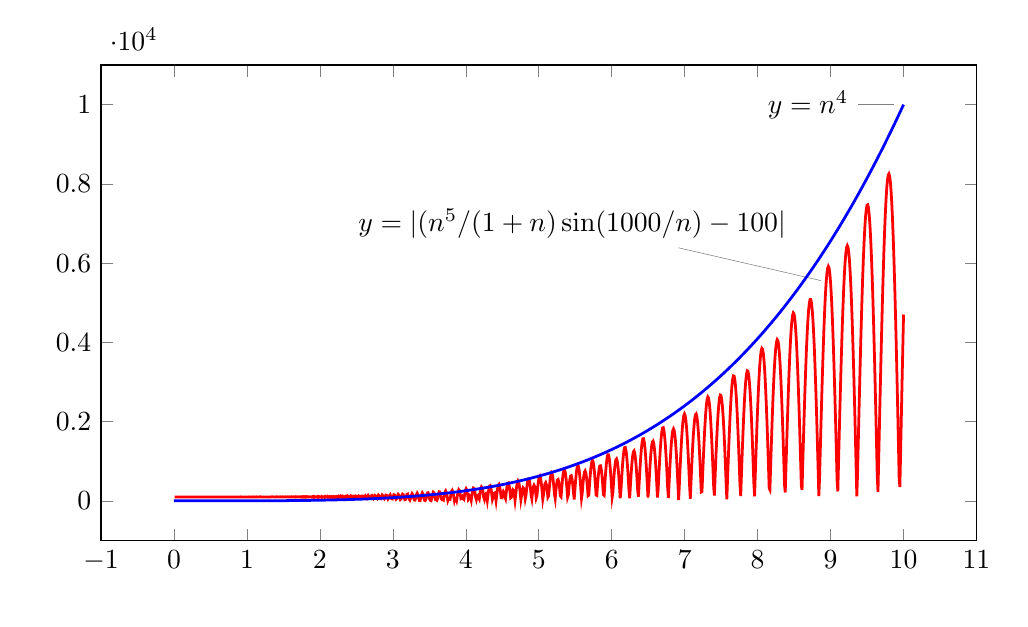
\begin{tikzpicture}[line width=1]
\begin{axis}[width=5in, height=3in,
             scatter/classes={a={mark=*,draw=black}},
             xlabel={\mbox{}},
             xlabel style={name=xlabel}, 
             ylabel={\mbox{}}, 
             legend style={
                at={(xlabel.south)},
                yshift=-1ex,
                anchor=north,
                legend cell align=left,
                },
        ]
]
\addplot[draw=red, line width=1] coordinates {(0.01,100.0)
(0.02,100.0)
(0.03,100.0)
(0.04,100.0)
(0.0501,100.0)
(0.0601,100.0)
(0.0701,100.0)
(0.0801,100.0)
(0.0901,100.0)
(0.1001,100.0)
(0.1101,100.0)
(0.1201,100.0)
(0.1301,100.0)
(0.1401,100.0)
(0.1502,100.0)
(0.1602,100.0001)
(0.1702,99.9999)
(0.1802,99.9999)
(0.1902,100.0002)
(0.2002,100.0)
(0.2102,99.9998)
(0.2202,100.0004)
(0.2302,99.9995)
(0.2402,99.9999)
(0.2503,100.0001)
(0.2603,100.0001)
(0.2703,100.0008)
(0.2803,100.0011)
(0.2903,99.9984)
(0.3003,100.0002)
(0.3103,100.0014)
(0.3203,100.0019)
(0.3303,100.0028)
(0.3403,100.0026)
(0.3504,99.9961)
(0.3604,100.0037)
(0.3704,100.005)
(0.3804,99.9969)
(0.3904,100.0059)
(0.4004,99.9995)
(0.4104,100.0079)
(0.4204,100.0035)
(0.4304,100.0103)
(0.4404,99.9909)
(0.4505,99.9886)
(0.4605,100.0111)
(0.4705,99.9848)
(0.4805,99.9827)
(0.4905,99.9978)
(0.5005,100.0011)
(0.5105,100.0229)
(0.5205,100.0251)
(0.5305,100.0014)
(0.5405,99.9884)
(0.5506,99.9837)
(0.5606,100.0169)
(0.5706,100.0142)
(0.5806,99.9695)
(0.5906,99.9956)
(0.6006,100.0022)
(0.6106,100.0424)
(0.6206,99.9807)
(0.6306,99.9565)
(0.6406,99.9723)
(0.6507,100.0447)
(0.6607,100.0435)
(0.6707,99.924)
(0.6807,100.0793)
(0.6907,99.9597)
(0.7007,99.9247)
(0.7107,100.0404)
(0.7207,100.0999)
(0.7307,100.1139)
(0.7407,100.0991)
(0.7508,100.0048)
(0.7608,99.861)
(0.7708,99.9885)
(0.7808,100.1372)
(0.7908,99.8277)
(0.8008,100.1828)
(0.8108,99.8129)
(0.8208,100.1231)
(0.8308,100.0811)
(0.8408,99.7759)
(0.8509,99.92)
(0.8609,100.1753)
(0.8709,100.2677)
(0.8809,100.2529)
(0.8909,100.2367)
(0.9009,100.2657)
(0.9109,100.3226)
(0.9209,100.3106)
(0.9309,100.083)
(0.9409,99.7005)
(0.951,99.6993)
(0.961,100.2872)
(0.971,100.2272)
(0.981,99.5422)
(0.991,100.2866)
(1.001,100.0133)
(1.011,99.7515)
(1.021,100.3803)
(1.031,99.5693)
(1.041,100.4085)
(1.0511,99.7145)
(1.0611,100.0163)
(1.0711,100.3797)
(1.0811,99.3044)
(1.0911,100.5463)
(1.1011,100.1992)
(1.1111,99.1996)
(1.1211,100.205)
(1.1311,100.8332)
(1.1411,99.8306)
(1.1512,99.0613)
(1.1612,99.6102)
(1.1712,100.6279)
(1.1812,101.0529)
(1.1912,100.6972)
(1.2012,99.9749)
(1.2112,99.316)
(1.2212,98.9084)
(1.2312,98.7374)
(1.2412,98.7051)
(1.2513,98.7135)
(1.2613,98.6972)
(1.2713,98.6291)
(1.2813,98.5218)
(1.2913,98.4333)
(1.3013,98.4725)
(1.3113,98.7831)
(1.3213,99.4779)
(1.3313,100.5081)
(1.3413,101.5244)
(1.3514,101.8936)
(1.3614,101.075)
(1.3714,99.3033)
(1.3814,97.9406)
(1.3914,98.5626)
(1.4014,100.9381)
(1.4114,102.315)
(1.4214,100.4658)
(1.4314,97.7263)
(1.4414,98.6852)
(1.4515,102.1477)
(1.4615,101.5752)
(1.4715,97.6395)
(1.4815,98.7688)
(1.4915,102.8627)
(1.5015,100.0538)
(1.5115,96.9846)
(1.5215,101.9416)
(1.5315,101.6252)
(1.5415,96.5773)
(1.5516,101.6573)
(1.5616,101.7388)
(1.5716,96.3051)
(1.5816,102.7984)
(1.5916,100.0656)
(1.6016,97.0887)
(1.6116,104.1607)
(1.6216,96.6112)
(1.6316,101.1842)
(1.6416,101.4311)
(1.6517,96.4487)
(1.6617,104.6718)
(1.6717,95.2906)
(1.6817,103.8715)
(1.6917,97.5104)
(1.7017,100.8896)
(1.7117,100.6794)
(1.7217,97.9346)
(1.7317,103.2022)
(1.7417,95.9153)
(1.7518,104.7427)
(1.7618,94.7808)
(1.7718,105.5553)
(1.7818,94.2201)
(1.7918,105.9045)
(1.8018,94.0809)
(1.8118,105.792)
(1.8218,94.5292)
(1.8318,104.8871)
(1.8418,96.0333)
(1.8519,102.6468)
(1.8619,99.0985)
(1.8719,98.7737)
(1.8819,103.5905)
(1.8919,94.0828)
(1.9019,107.8044)
(1.9119,91.2332)
(1.9219,108.3379)
(1.9319,93.7686)
(1.9419,102.5287)
(1.952,102.1706)
(1.962,93.268)
(1.972,109.6948)
(1.982,90.2638)
(1.992,106.3004)
(2.002,99.8583)
(2.012,93.4337)
(2.022,110.8471)
(2.032,89.7559)
(2.042,104.3574)
(2.0521,104.3135)
(2.0621,88.9055)
(2.0721,111.573)
(2.0821,95.3475)
(2.0921,94.1491)
(2.1021,112.8617)
(2.1121,89.2482)
(2.1221,100.1721)
(2.1321,111.165)
(2.1421,86.2686)
(2.1522,104.3922)
(2.1622,109.4646)
(2.1722,84.875)
(2.1822,106.2788)
(2.1922,109.388)
(2.2022,83.9634)
(2.2122,105.7045)
(2.2222,111.4917)
(2.2322,83.6447)
(2.2422,102.1623)
(2.2523,115.3265)
(2.2623,85.449)
(2.2723,95.1491)
(2.2823,118.7818)
(2.2923,91.8666)
(2.3023,85.839)
(2.3123,117.5281)
(2.3223,104.1439)
(2.3323,79.3426)
(2.3423,106.9063)
(2.3524,117.9793)
(2.3624,84.1523)
(2.3724,88.4371)
(2.3824,121.3509)
(2.3924,103.6763)
(2.4024,76.4811)
(2.4124,103.9897)
(2.4224,123.2152)
(2.4324,89.4886)
(2.4424,78.4954)
(2.4525,115.5909)
(2.4625,119.3337)
(2.4725,80.691)
(2.4825,82.5854)
(2.4925,121.8984)
(2.5025,116.2298)
(2.5125,76.4175)
(2.5225,83.9191)
(2.5325,124.476)
(2.5425,117.1332)
(2.5526,75.4692)
(2.5626,80.5715)
(2.5726,123.5181)
(2.5826,122.8565)
(2.5926,78.9562)
(2.6026,72.9149)
(2.6126,116.6155)
(2.6226,131.4681)
(2.6326,90.2189)
(2.6426,65.0309)
(2.6527,100.3591)
(2.6627,136.1652)
(2.6727,111.2488)
(2.6827,66.5771)
(2.6927,76.269)
(2.7027,125.3258)
(2.7127,134.6763)
(2.7227,88.6249)
(2.7327,59.2491)
(2.7427,92.829)
(2.7528,138.4801)
(2.7628,126.6767)
(2.7728,74.2894)
(2.7828,58.7105)
(2.7928,103.4479)
(2.8028,144.4373)
(2.8128,122.7875)
(2.8228,68.2253)
(2.8328,56.6493)
(2.8428,104.7187)
(2.8529,147.6561)
(2.8629,127.4459)
(2.8729,70.1016)
(2.8829,50.5877)
(2.8929,94.8274)
(2.9029,146.8884)
(2.9129,140.805)
(2.9229,83.3933)
(2.9329,45.056)
(2.9429,72.9663)
(2.953,134.2823)
(2.963,156.2209)
(2.973,112.3702)
(2.983,52.9834)
(2.993,46.2618)
(3.003,100.5382)
(3.013,155.5643)
(3.023,150.2114)
(3.033,89.593)
(3.043,38.7764)
(3.0531,52.357)
(3.0631,116.7428)
(3.0731,165.158)
(3.0831,147.3267)
(3.0931,80.6805)
(3.1031,31.9667)
(3.1131,50.034)
(3.1231,117.8389)
(3.1331,169.8365)
(3.1431,155.726)
(3.1532,88.1914)
(3.1632,30.2144)
(3.1732,35.861)
(3.1832,100.6502)
(3.1932,166.3266)
(3.2032,173.8673)
(3.2132,115.9348)
(3.2232,42.7)
(3.2332,17.5855)
(3.2432,62.665)
(3.2533,140.4329)
(3.2633,185.9931)
(3.2733,161.2194)
(3.2833,85.6927)
(3.2933,20.1203)
(3.3033,17.1679)
(3.3133,79.8156)
(3.3233,159.6335)
(3.3333,194.9436)
(3.3433,158.2441)
(3.3534,76.6251)
(3.3634,10.7952)
(3.3734,9.6847)
(3.3834,74.739)
(3.3934,159.4614)
(3.4034,203.329)
(3.4134,174.8611)
(3.4234,93.3229)
(3.4334,14.7371)
(3.4434,6.9867)
(3.4535,43.415)
(3.4635,132.8045)
(3.4735,202.2344)
(3.4835,205.9565)
(3.4935,140.9551)
(3.5035,48.3478)
(3.5135,13.2874)
(3.5235,4.9412)
(3.5335,68.8218)
(3.5435,163.2172)
(3.5536,220.9944)
(3.5636,207.0542)
(3.5736,129.0734)
(3.5836,32.4443)
(3.5936,26.6619)
(3.6036,13.8306)
(3.6136,64.2283)
(3.6236,163.9863)
(3.6336,229.8827)
(3.6436,225.1968)
(3.6537,151.9038)
(3.6637,49.1185)
(3.6737,28.3288)
(3.6837,39.1637)
(3.6937,22.8438)
(3.7037,126.0836)
(3.7137,217.8269)
(3.7237,251.3134)
(3.7337,209.2176)
(3.7437,111.9136)
(3.7538,6.9539)
(3.7638,54.4841)
(3.7738,42.3722)
(3.7838,38.071)
(3.7938,149.2919)
(3.8038,239.4049)
(3.8138,266.4424)
(3.8238,217.5042)
(3.8338,114.2599)
(3.8438,2.7648)
(3.8539,67.3644)
(3.8639,64.8811)
(3.8739,9.6737)
(3.8839,124.6003)
(3.8939,230.9981)
(3.9039,283.706)
(3.9139,260.2091)
(3.9239,169.7138)
(3.9339,48.9672)
(3.9439,53.0556)
(3.954,95.06)
(3.964,59.8343)
(3.974,39.239)
(3.984,163.8028)
(3.994,265.7136)
(4.004,305.6579)
(4.014,268.0019)
(4.024,166.3913)
(4.034,38.2997)
(4.044,69.1136)
(4.0541,116.3856)
(4.0641,85.9629)
(4.0741,11.7625)
(4.0841,142.4905)
(4.0941,260.3889)
(4.1041,324.2276)
(4.1141,311.5746)
(4.1241,226.2484)
(4.1341,96.7038)
(4.1441,33.8274)
(4.1542,121.9046)
(4.1642,138.2051)
(4.1742,76.9314)
(4.1842,42.5969)
(4.1942,182.4395)
(4.2042,298.3106)
(4.2142,353.5915)
(4.2242,330.6551)
(4.2342,236.0829)
(4.2442,98.3609)
(4.2543,41.0217)
(4.2643,140.194)
(4.2743,169.3743)
(4.2843,119.5117)
(4.2943,4.685)
(4.3043,142.2508)
(4.3143,279.3187)
(4.3243,367.4679)
(4.3343,381.547)
(4.3443,317.1653)
(4.3544,191.6625)
(4.3644,39.0954)
(4.3744,99.2193)
(4.3844,185.9235)
(4.3944,197.5483)
(4.4044,130.5626)
(4.4144,2.0652)
(4.4244,154.9025)
(4.4344,300.0578)
(4.4444,396.2519)
(4.4545,418.8378)
(4.4645,361.7112)
(4.4745,238.6124)
(4.4845,79.5078)
(4.4945,76.923)
(4.5045,192.7602)
(4.5145,239.9437)
(4.5245,206.8396)
(4.5345,100.7975)
(4.5445,53.7886)
(4.5546,221.3355)
(4.5646,363.3827)
(4.5746,447.3955)
(4.5846,454.0514)
(4.5946,381.4195)
(4.6046,245.1909)
(4.6146,75.0207)
(4.6246,92.1093)
(4.6346,219.9834)
(4.6446,280.9209)
(4.6547,261.5729)
(4.6647,165.5791)
(4.6747,12.6129)
(4.6847,165.8837)
(4.6947,333.3053)
(4.7047,455.4141)
(4.7147,507.2435)
(4.7247,478.0062)
(4.7347,373.0822)
(4.7447,212.7758)
(4.7548,28.1733)
(4.7648,145.0128)
(4.7748,273.3724)
(4.7848,332.1524)
(4.7948,309.8484)
(4.8048,210.2191)
(4.8148,51.4161)
(4.8248,137.5289)
(4.8348,322.1453)
(4.8448,468.85)
(4.8549,550.9924)
(4.8649,553.5444)
(4.8749,475.6387)
(4.8849,330.5656)
(4.8949,143.2986)
(4.9049,53.9576)
(4.9149,227.3763)
(4.9249,347.2903)
(4.9349,393.1595)
(4.9449,356.9155)
(4.955,244.1682)
(4.965,73.1315)
(4.975,128.4941)
(4.985,328.1222)
(4.995,493.5829)
(5.005,598.2596)
(5.015,625.2496)
(5.025,569.9188)
(5.035,440.4934)
(5.045,256.6479)
(5.0551,46.3603)
(5.0651,158.4425)
(5.0751,326.7551)
(5.0851,433.1376)
(5.0951,461.4444)
(5.1051,407.1111)
(5.1151,277.7012)
(5.1251,91.677)
(5.1351,124.3808)
(5.1451,339.6664)
(5.1552,523.5725)
(5.1652,650.0059)
(5.1752,700.992)
(5.1852,669.0871)
(5.1952,558.2938)
(5.2052,383.3936)
(5.2152,167.8279)
(5.2252,59.5512)
(5.2352,268.3947)
(5.2452,430.9003)
(5.2553,525.4468)
(5.2653,539.3571)
(5.2753,470.4494)
(5.2853,327.2099)
(5.2953,127.5982)
(5.3053,103.3283)
(5.3153,336.642)
(5.3253,543.1995)
(5.3353,697.2584)
(5.3453,779.6115)
(5.3554,779.8667)
(5.3654,697.6176)
(5.3754,542.3905)
(5.3854,332.4048)
(5.3954,92.3232)
(5.4054,149.718)
(5.4154,365.4332)
(5.4254,529.6712)
(5.4354,623.2809)
(5.4454,635.2404)
(5.4555,563.8268)
(5.4655,416.7162)
(5.4755,210.0311)
(5.4855,33.536)
(5.4955,287.2897)
(5.5055,523.495)
(5.5155,716.4016)
(5.5255,845.003)
(5.5355,895.2392)
(5.5455,861.4236)
(5.5556,746.7601)
(5.5656,562.9189)
(5.5756,328.7378)
(5.5856,68.2046)
(5.5956,192.0561)
(5.6056,425.5216)
(5.6156,608.4537)
(5.6256,722.2564)
(5.6356,755.2801)
(5.6456,703.9079)
(5.6557,572.8322)
(5.6657,374.516)
(5.6757,127.9074)
(5.6857,143.4476)
(5.6957,413.702)
(5.7057,657.1849)
(5.7157,850.8205)
(5.7257,976.2641)
(5.7357,1021.5625)
(5.7457,982.1965)
(5.7558,861.4232)
(5.7658,669.9049)
(5.7758,424.6732)
(5.7858,147.5376)
(5.7958,136.9059)
(5.8058,403.4815)
(5.8158,628.6542)
(5.8258,792.5717)
(5.8358,880.7525)
(5.8458,885.2833)
(5.8559,805.4341)
(5.8659,647.6526)
(5.8759,424.9509)
(5.8859,155.7521)
(5.8959,137.6967)
(5.9059,431.2014)
(5.9159,700.6293)
(5.9259,923.8786)
(5.9359,1082.6529)
(5.9459,1163.8995)
(5.956,1160.805)
(5.966,1073.2786)
(5.976,907.8968)
(5.986,677.3248)
(5.996,399.2733)
(6.006,95.0801)
(6.016,211.9644)
(6.026,498.4143)
(6.036,742.4492)
(6.046,925.5042)
(6.0561,1033.6299)
(6.0661,1058.4883)
(6.0761,997.9168)
(6.0861,856.0307)
(6.0961,642.8651)
(6.1061,373.5935)
(6.1161,67.3878)
(6.1261,253.9891)
(6.1361,567.7541)
(6.1461,851.7221)
(6.1562,1085.8563)
(6.1662,1253.6457)
(6.1762,1343.2166)
(6.1862,1348.1071)
(6.1962,1267.6603)
(6.2062,1107.0161)
(6.2162,876.7122)
(6.2262,591.9288)
(6.2362,271.4353)
(6.2462,63.6846)
(6.2563,391.4404)
(6.2663,690.3803)
(6.2763,940.9798)
(6.2863,1126.8847)
(6.2963,1235.931)
(6.3063,1260.883)
(6.3163,1199.8477)
(6.3263,1056.3463)
(6.3363,839.0459)
(6.3463,561.1756)
(6.3564,239.6689)
(6.3664,105.9074)
(6.3764,454.5703)
(6.3864,785.2036)
(6.3964,1077.8314)
(6.4064,1314.8029)
(6.4164,1481.822)
(6.4264,1568.7624)
(6.4364,1570.2264)
(6.4464,1485.8181)
(6.4565,1320.1229)
(6.4665,1082.3998)
(6.4765,786.0103)
(6.4865,447.6213)
(6.4965,86.2338)
(6.5065,277.9063)
(6.5165,624.4512)
(6.5265,934.0821)
(6.5365,1189.5674)
(6.5465,1376.6908)
(6.5566,1485.0002)
(6.5666,1508.3429)
(6.5766,1445.1595)
(6.5866,1298.5285)
(6.5966,1075.9625)
(6.6066,788.9728)
(6.6166,452.4296)
(6.6266,83.756)
(6.6366,297.9995)
(6.6466,673.1604)
(6.6567,1022.4384)
(6.6667,1327.9144)
(6.6767,1573.9362)
(6.6867,1747.8884)
(6.6967,1840.7998)
(6.7067,1847.7589)
(6.7167,1768.1241)
(6.7267,1605.5182)
(6.7367,1367.616)
(6.7467,1065.7367)
(6.7568,714.2655)
(6.7668,329.9361)
(6.7768,68.9885)
(6.7868,463.5974)
(6.7968,835.2301)
(6.8068,1166.3514)
(6.8168,1441.3606)
(6.8268,1647.3)
(6.8368,1774.4306)
(6.8468,1816.6526)
(6.8569,1771.7533)
(6.8669,1641.4757)
(6.8769,1431.407)
(6.8869,1150.6966)
(6.8969,811.619)
(6.9069,429.0041)
(6.9169,19.5631)
(6.9269,398.8589)
(6.9369,808.0693)
(6.9469,1190.3187)
(6.957,1529.0612)
(6.967,1809.653)
(6.977,2019.9598)
(6.987,2150.8501)
(6.997,2196.5552)
(7.007,2154.8827)
(7.017,2027.2793)
(7.027,1818.741)
(7.037,1537.5795)
(7.047,1195.0553)
(7.0571,804.8959)
(7.0671,382.7213)
(7.0771,54.5992)
(7.0871,489.6318)
(7.0971,905.0753)
(7.1071,1284.444)
(7.1171,1612.7094)
(7.1271,1876.8756)
(7.1371,2066.4685)
(7.1471,2173.9204)
(7.1572,2194.8377)
(7.1672,2128.1438)
(7.1772,1976.0935)
(7.1872,1744.1613)
(7.1972,1440.8107)
(7.2072,1077.1534)
(7.2172,666.516)
(7.2272,223.9298)
(7.2372,234.4355)
(7.2472,691.8714)
(7.2573,1131.743)
(7.2673,1538.0891)
(7.2773,1896.1916)
(7.2873,2193.0916)
(7.2973,2418.0368)
(7.3073,2562.8448)
(7.3173,2622.1705)
(7.3273,2593.6712)
(7.3373,2478.0649)
(7.3473,2279.0816)
(7.3574,2003.3115)
(7.3674,1659.9574)
(7.3774,1260.5008)
(7.3874,818.296)
(7.3974,348.1055)
(7.4074,134.4053)
(7.4174,613.197)
(7.4274,1072.3903)
(7.4374,1496.789)
(7.4474,1872.3719)
(7.4575,2186.7417)
(7.4675,2429.5146)
(7.4775,2592.6398)
(7.4875,2670.6399)
(7.4975,2660.7665)
(7.5075,2563.0662)
(7.5175,2380.3582)
(7.5275,2118.1249)
(7.5375,1784.3197)
(7.5475,1389.1018)
(7.5576,944.5052)
(7.5676,464.0542)
(7.5776,37.6612)
(7.5876,545.4374)
(7.5976,1043.9219)
(7.6076,1518.0771)
(7.6176,1953.6277)
(7.6276,2337.4809)
(7.6376,2658.1053)
(7.6476,2905.8591)
(7.6577,3073.2591)
(7.6677,3155.1827)
(7.6777,3148.999)
(7.6877,3054.6262)
(7.6977,2874.5152)
(7.7077,2613.5606)
(7.7177,2278.9431)
(7.7277,1879.9103)
(7.7377,1427.5004)
(7.7477,934.2203)
(7.7578,413.6868)
(7.7678,119.7591)
(7.7778,651.4529)
(7.7878,1166.8108)
(7.7978,1651.7267)
(7.8078,2092.9521)
(7.8178,2478.4471)
(7.8278,2797.6951)
(7.8378,3041.9724)
(7.8478,3204.5675)
(7.8579,3280.9439)
(7.8679,3268.8431)
(7.8779,3168.328)
(7.8879,2981.7636)
(7.8979,2713.7394)
(7.9079,2370.9351)
(7.9179,1961.9334)
(7.9279,1496.9877)
(7.9379,987.7496)
(7.9479,446.9637)
(7.958,111.86)
(7.968,674.79)
(7.978,1227.8233)
(7.988,1757.2324)
(7.998,2249.9018)
(8.008,2693.6456)
(8.018,3077.4974)
(8.028,3391.9688)
(8.038,3629.2672)
(8.048,3783.4716)
(8.0581,3850.6607)
(8.0681,3828.9918)
(8.0781,3718.7302)
(8.0881,3522.2273)
(8.0981,3243.8511)
(8.1081,2889.8701)
(8.1181,2468.2937)
(8.1281,1988.6756)
(8.1381,1461.8826)
(8.1481,899.8372)
(8.1582,315.2384)
(8.1682,278.7313)
(8.1782,868.7064)
(8.1882,1441.4397)
(8.1982,1984.0972)
(8.2082,2484.5402)
(8.2182,2931.5888)
(8.2282,3315.2613)
(8.2382,3626.9842)
(8.2482,3859.7693)
(8.2583,4008.3543)
(8.2683,4069.3038)
(8.2783,4041.071)
(8.2883,3924.0174)
(8.2983,3720.3917)
(8.3083,3434.2696)
(8.3183,3071.4548)
(8.3283,2639.3457)
(8.3383,2146.77)
(8.3483,1603.7917)
(8.3584,1021.4945)
(8.3684,411.7469)
(8.3784,213.046)
(8.3884,840.199)
(8.3984,1457.0054)
(8.4084,2050.9941)
(8.4184,2610.1779)
(8.4284,3123.2898)
(8.4384,3580.0025)
(8.4484,3971.1259)
(8.4585,4288.7808)
(8.4685,4526.5441)
(8.4785,4679.5647)
(8.4885,4744.6465)
(8.4985,4720.2997)
(8.5085,4606.7571)
(8.5185,4405.9584)
(8.5285,4121.502)
(8.5385,3758.5647)
(8.5485,3323.7943)
(8.5586,2825.1741)
(8.5686,2271.8646)
(8.5786,1674.0256)
(8.5886,1042.6205)
(8.5986,389.2092)
(8.6086,274.2684)
(8.6186,935.713)
(8.6286,1583.0872)
(8.6386,2204.6326)
(8.6486,2789.0806)
(8.6587,3325.8505)
(8.6687,3805.2345)
(8.6787,4218.5638)
(8.6887,4558.3557)
(8.6987,4818.437)
(8.7087,4994.0438)
(8.7187,5081.8954)
(8.7287,5080.2412)
(8.7387,4988.8809)
(8.7487,4809.1581)
(8.7588,4543.9264)
(8.7688,4197.4917)
(8.7788,3775.5288)
(8.7888,3284.9769)
(8.7988,2733.9144)
(8.8088,2131.4163)
(8.8188,1487.3963)
(8.8288,812.4369)
(8.8388,117.6102)
(8.8488,585.7074)
(8.8589,1286.0235)
(8.8689,1971.9175)
(8.8789,2632.2255)
(8.8889,3256.2192)
(8.8989,3833.7751)
(8.9089,4355.5328)
(8.9189,4813.0394)
(8.9289,5198.8771)
(8.9389,5506.7746)
(8.9489,5731.6974)
(8.959,5869.9189)
(8.969,5919.0703)
(8.979,5878.1682)
(8.989,5747.6213)
(8.999,5529.2146)
(9.009,5226.074)
(9.019,4842.6093)
(9.029,4384.4398)
(9.039,3858.3012)
(9.049,3271.9374)
(9.0591,2633.9782)
(9.0691,1953.8049)
(9.0791,1241.4065)
(9.0891,507.228)
(9.0991,237.9858)
(9.1091,983.3496)
(9.1191,1717.9973)
(9.1291,2431.2395)
(9.1391,3112.7168)
(9.1491,3752.5469)
(9.1592,4341.4631)
(9.1692,4870.9425)
(9.1792,5333.3222)
(9.1892,5721.9027)
(9.1992,6031.0355)
(9.2092,6256.1964)
(9.2192,6394.0408)
(9.2292,6442.4435)
(9.2392,6400.5198)
(9.2492,6268.6306)
(9.2593,6048.3689)
(9.2693,5742.531)
(9.2793,5355.071)
(9.2893,4891.0393)
(9.2993,4356.5085)
(9.3093,3758.4852)
(9.3193,3104.8108)
(9.3293,2404.0514)
(9.3393,1665.3806)
(9.3493,898.4541)
(9.3594,113.2802)
(9.3694,679.9134)
(9.3794,1470.8142)
(9.3894,2249.159)
(9.3994,3004.8663)
(9.4094,3728.1648)
(9.4194,4409.7164)
(9.4294,5040.733)
(9.4394,5613.0843)
(9.4494,6119.3966)
(9.4595,6553.1412)
(9.4695,6908.7112)
(9.4795,7181.4852)
(9.4895,7367.8793)
(9.4995,7465.3852)
(9.5095,7472.594)
(9.5195,7389.2074)
(9.5295,7216.034)
(9.5395,6954.9736)
(9.5495,6608.9865)
(9.5596,6182.0521)
(9.5696,5679.1147)
(9.5796,5106.0185)
(9.5896,4469.4322)
(9.5996,3776.7655)
(9.6096,3036.0765)
(9.6196,2255.9732)
(9.6296,1445.5093)
(9.6396,614.0757)
(9.6496,228.7105)
(9.6597,1073.1189)
(9.6697,1909.4183)
(9.6797,2727.9888)
(9.6897,3519.4309)
(9.6997,4274.6713)
(9.7097,4985.0636)
(9.7197,5642.4839)
(9.7297,6239.4183)
(9.7397,6769.0442)
(9.7497,7225.3016)
(9.7598,7602.9564)
(9.7698,7897.6532)
(9.7798,8105.9578)
(9.7898,8225.3899)
(9.7998,8254.4442)
(9.8098,8192.6014)
(9.8198,8040.3273)
(9.8298,7799.0629)
(9.8398,7471.2023)
(9.8498,7060.0619)
(9.8599,6569.8398)
(9.8699,6005.5653)
(9.8799,5373.0417)
(9.8899,4678.78)
(9.8999,3929.9268)
(9.9099,3134.1856)
(9.9199,2299.7338)
(9.9299,1435.1346)
(9.9399,549.2471)
(9.9499,348.8674)
(9.96,1250.0385)
(9.97,2145.0815)
(9.98,3024.8905)
(9.99,3880.5299)
(10.0,4703.324)
(10.0,4703.324)};\node[pin=above left:{$y=|(n^5/(1 + n) \sin(1000/n) - 100|$}] at (axis cs:9,5502.650667563646) {};\addplot[draw=blue, line width=1] coordinates {(0.0,0.0)
(0.0503,0.0)
(0.1005,0.0001)
(0.1508,0.0005)
(0.201,0.0016)
(0.2513,0.004)
(0.3015,0.0083)
(0.3518,0.0153)
(0.402,0.0261)
(0.4523,0.0418)
(0.5025,0.0638)
(0.5528,0.0934)
(0.603,0.1322)
(0.6533,0.1821)
(0.7035,0.245)
(0.7538,0.3228)
(0.804,0.4179)
(0.8543,0.5326)
(0.9045,0.6694)
(0.9548,0.831)
(1.005,1.0203)
(1.0553,1.2401)
(1.1055,1.4938)
(1.1558,1.7844)
(1.206,2.1156)
(1.2563,2.4909)
(1.3065,2.9139)
(1.3568,3.3888)
(1.407,3.9194)
(1.4573,4.51)
(1.5075,5.165)
(1.5578,5.8889)
(1.608,6.6863)
(1.6583,7.5621)
(1.7085,8.5213)
(1.7588,9.5689)
(1.809,10.7102)
(1.8593,11.9507)
(1.9095,13.296)
(1.9598,14.7518)
(2.0101,16.324)
(2.0603,18.0187)
(2.1106,19.842)
(2.1608,21.8003)
(2.2111,23.9)
(2.2613,26.148)
(2.3116,28.5508)
(2.3618,31.1157)
(2.4121,33.8495)
(2.4623,36.7597)
(2.5126,39.8536)
(2.5628,43.1388)
(2.6131,46.6231)
(2.6633,50.3143)
(2.7136,54.2204)
(2.7638,58.3497)
(2.8141,62.7104)
(2.8643,67.3112)
(2.9146,72.1605)
(2.9648,77.2673)
(3.0151,82.6405)
(3.0653,88.2891)
(3.1156,94.2225)
(3.1658,100.45)
(3.2161,106.9812)
(3.2663,113.8259)
(3.3166,120.9939)
(3.3668,128.4952)
(3.4171,136.34)
(3.4673,144.5387)
(3.5176,153.1016)
(3.5678,162.0396)
(3.6181,171.3632)
(3.6683,181.0836)
(3.7186,191.2117)
(3.7688,201.7589)
(3.8191,212.7365)
(3.8693,224.1561)
(3.9196,236.0294)
(3.9698,248.3682)
(4.0201,261.1846)
(4.0704,274.4908)
(4.1206,288.299)
(4.1709,302.6217)
(4.2211,317.4716)
(4.2714,332.8614)
(4.3216,348.804)
(4.3719,365.3126)
(4.4221,382.4004)
(4.4724,400.0808)
(4.5226,418.3673)
(4.5729,437.2736)
(4.6231,456.8136)
(4.6734,477.0012)
(4.7236,497.8507)
(4.7739,519.3763)
(4.8241,541.5925)
(4.8744,564.5139)
(4.9246,588.1553)
(4.9749,612.5316)
(5.0251,637.6578)
(5.0754,663.5493)
(5.1256,690.2213)
(5.1759,717.6895)
(5.2261,745.9695)
(5.2764,775.0771)
(5.3266,805.0283)
(5.3769,835.8393)
(5.4271,867.5264)
(5.4774,900.1061)
(5.5276,933.5948)
(5.5779,968.0095)
(5.6281,1003.3669)
(5.6784,1039.6843)
(5.7286,1076.9787)
(5.7789,1115.2675)
(5.8291,1154.5684)
(5.8794,1194.8988)
(5.9296,1236.2768)
(5.9799,1278.7202)
(6.0302,1322.2473)
(6.0804,1366.8762)
(6.1307,1412.6254)
(6.1809,1459.5136)
(6.2312,1507.5594)
(6.2814,1556.7818)
(6.3317,1607.1998)
(6.3819,1658.8327)
(6.4322,1711.6997)
(6.4824,1765.8204)
(6.5327,1821.2145)
(6.5829,1877.9018)
(6.6332,1935.9022)
(6.6834,1995.2359)
(6.7337,2055.9232)
(6.7839,2117.9845)
(6.8342,2181.4403)
(6.8844,2246.3114)
(6.9347,2312.6187)
(6.9849,2380.3833)
(7.0352,2449.6263)
(7.0854,2520.3691)
(7.1357,2592.6332)
(7.1859,2666.4402)
(7.2362,2741.8119)
(7.2864,2818.7704)
(7.3367,2897.3377)
(7.3869,2977.5361)
(7.4372,3059.388)
(7.4874,3142.916)
(7.5377,3228.1427)
(7.5879,3315.0912)
(7.6382,3403.7844)
(7.6884,3494.2455)
(7.7387,3586.4979)
(7.7889,3680.565)
(7.8392,3776.4704)
(7.8894,3874.2381)
(7.9397,3973.8918)
(7.9899,4075.4558)
(8.0402,4178.9543)
(8.0905,4284.4117)
(8.1407,4391.8526)
(8.191,4501.3016)
(8.2412,4612.7837)
(8.2915,4726.3238)
(8.3417,4841.9472)
(8.392,4959.6791)
(8.4422,5079.5451)
(8.4925,5201.5708)
(8.5427,5325.7819)
(8.593,5452.2045)
(8.6432,5580.8645)
(8.6935,5711.7884)
(8.7437,5845.0023)
(8.794,5980.533)
(8.8442,6118.407)
(8.8945,6258.6514)
(8.9447,6401.293)
(8.995,6546.359)
(9.0452,6693.8768)
(9.0955,6843.8738)
(9.1457,6996.3777)
(9.196,7151.4162)
(9.2462,7309.0172)
(9.2965,7469.2089)
(9.3467,7632.0195)
(9.397,7797.4773)
(9.4472,7965.611)
(9.4975,8136.4491)
(9.5477,8310.0206)
(9.598,8486.3544)
(9.6482,8665.4797)
(9.6985,8847.4258)
(9.7487,9032.2222)
(9.799,9219.8985)
(9.8492,9410.4844)
(9.8995,9604.0099)
(9.9497,9800.505)
(10.0,10000.0)};\node[pin=left:{$y=n^4$}] at (axis cs:10,10000) {};
\end{axis}\end{tikzpicture}\end{center}


You notice that $g(n)$ beats $|f(n)|$ around 
$5 \leq n \leq 6.5$.
Let me zoom in.
Here's the plot for $3 \leq n \leq 7$:
%-*-latex-*-

\begin{center}
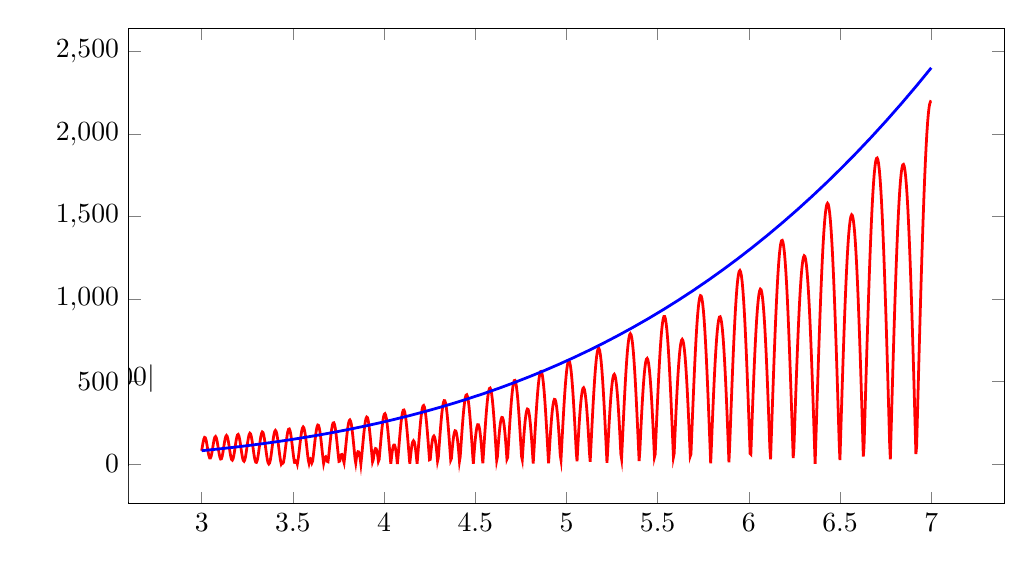
\begin{tikzpicture}[line width=1]
\begin{axis}[width=5in, height=3in,
             scatter/classes={a={mark=*,draw=black}},
             xlabel={\mbox{}},
             xlabel style={name=xlabel}, 
             ylabel={\mbox{}}, 
             legend style={
                at={(xlabel.south)},
                yshift=-1ex,
                anchor=north,
                legend cell align=left,
                },
        ]
]
\addplot[draw=red, line width=1] coordinates {(3.0,80.6301)
(3.004,107.3008)
(3.008,132.7879)
(3.012,152.1556)
(3.016,161.6538)
(3.02,159.4284)
(3.024,145.8614)
(3.028,123.483)
(3.032,96.4803)
(3.036,69.9005)
(3.04,48.7036)
(3.044,36.8426)
(3.048,36.5403)
(3.0521,47.8931)
(3.0561,68.8678)
(3.0601,95.6852)
(3.0641,123.5163)
(3.0681,147.3573)
(3.0721,162.9271)
(3.0761,167.4241)
(3.0801,160.0131)
(3.0841,141.9589)
(3.0881,116.3902)
(3.0921,87.7417)
(3.0961,60.975)
(3.1001,40.7188)
(3.1041,30.4755)
(3.1081,32.0305)
(3.1121,45.16)
(3.1161,67.6821)
(3.1201,95.8374)
(3.1241,124.9296)
(3.1281,150.1137)
(3.1321,167.2007)
(3.1361,173.3442)
(3.1401,167.4988)
(3.1441,150.5785)
(3.1481,125.2953)
(3.1522,95.7087)
(3.1562,66.5638)
(3.1602,42.5272)
(3.1642,27.4442)
(3.1682,23.7351)
(3.1722,32.0227)
(3.1762,51.0469)
(3.1802,77.8734)
(3.1842,108.361)
(3.1882,137.8095)
(3.1922,161.686)
(3.1962,176.3181)
(3.2002,179.4469)
(3.2042,170.5604)
(3.2082,150.9589)
(3.2122,123.5483)
(3.2162,92.3955)
(3.2202,62.1167)
(3.2242,37.1912)
(3.2282,21.3035)
(3.2322,16.809)
(3.2362,24.3995)
(3.2402,43.0139)
(3.2442,70.0026)
(3.2482,101.5182)
(3.2523,133.0731)
(3.2563,160.1813)
(3.2603,178.9934)
(3.2643,186.8342)
(3.2683,182.5699)
(3.2723,166.7562)
(3.2763,141.5504)
(3.2803,110.4031)
(3.2843,77.5755)
(3.2883,47.5516)
(3.2923,24.4266)
(3.2963,11.3545)
(3.3003,10.1293)
(3.3043,20.9528)
(3.3083,42.4179)
(3.3123,71.7064)
(3.3163,104.9699)
(3.3203,137.8434)
(3.3243,166.0202)
(3.3283,185.8126)
(3.3323,194.6268)
(3.3363,191.2905)
(3.3403,176.1945)
(3.3443,151.2328)
(3.3483,119.5522)
(3.3524,85.145)
(3.3564,52.3413)
(3.3604,25.2625)
(3.3644,7.3084)
(3.3684,0.739)
(3.3724,6.4023)
(3.3764,23.6384)
(3.3804,50.3701)
(3.3844,83.3656)
(3.3884,118.6375)
(3.3924,151.9301)
(3.3964,179.2324)
(3.4004,197.2574)
(3.4044,203.8288)
(3.4084,198.1324)
(3.4124,180.8035)
(3.4164,153.8434)
(3.4204,120.3766)
(3.4244,84.28)
(3.4284,49.7289)
(3.4324,20.7136)
(3.4364,0.5824)
(3.4404,8.3373)
(3.4444,4.9971)
(3.4484,10.2613)
(3.4525,35.7536)
(3.4565,68.6498)
(3.4605,105.2979)
(3.4645,141.6345)
(3.4685,173.6374)
(3.4725,197.7682)
(3.4765,211.3574)
(3.4805,212.8906)
(3.4845,202.1656)
(3.4885,180.3064)
(3.4925,149.634)
(3.4965,113.4102)
(3.5005,75.4839)
(3.5045,39.8785)
(3.5085,10.3655)
(3.5125,9.9307)
(3.5165,18.8568)
(3.5205,15.4484)
(3.5245,0.0237)
(3.5285,25.8576)
(3.5325,59.5624)
(3.5365,97.6605)
(3.5405,136.2791)
(3.5445,171.4987)
(3.5485,199.7499)
(3.5526,218.1699)
(3.5566,224.8853)
(3.5606,219.1929)
(3.5646,201.6223)
(3.5686,173.8762)
(3.5726,138.6559)
(3.5766,99.3902)
(3.5806,59.8971)
(3.5846,24.0105)
(3.5886,4.7904)
(3.5926,23.7139)
(3.5966,30.9188)
(3.6006,25.6848)
(3.6046,8.4739)
(3.6086,19.1203)
(3.6126,54.5295)
(3.6166,94.4571)
(3.6206,135.1902)
(3.6246,172.9471)
(3.6286,204.2271)
(3.6326,226.1318)
(3.6366,236.6266)
(3.6406,234.7218)
(3.6446,220.556)
(3.6486,195.377)
(3.6527,161.4229)
(3.6567,121.715)
(3.6607,79.7841)
(3.6647,39.3526)
(3.6687,4.0047)
(3.6727,23.1296)
(3.6767,39.6459)
(3.6807,44.0716)
(3.6847,35.9883)
(3.6887,16.0623)
(3.6927,14.0198)
(3.6967,51.7017)
(3.7007,93.7812)
(3.7047,136.6867)
(3.7087,176.782)
(3.7127,210.6742)
(3.7167,235.497)
(3.7207,249.1478)
(3.7247,250.4585)
(3.7287,239.2871)
(3.7327,216.523)
(3.7367,184.0086)
(3.7407,144.3819)
(3.7447,100.8571)
(3.7487,56.9603)
(3.7528,16.2418)
(3.7568,18.0094)
(3.7608,43.0283)
(3.7648,56.7919)
(3.7688,58.1751)
(3.7728,47.0357)
(3.7768,24.2188)
(3.7808,8.5143)
(3.7848,48.6298)
(3.7888,93.0229)
(3.7928,138.2618)
(3.7968,180.8549)
(3.8008,217.5193)
(3.8048,245.4316)
(3.8088,262.4398)
(3.8128,267.2237)
(3.8168,259.3893)
(3.8208,239.4936)
(3.8248,208.9974)
(3.8288,170.1507)
(3.8328,125.8212)
(3.8368,79.2783)
(3.8408,33.9493)
(3.8448,6.8327)
(3.8488,40.0725)
(3.8529,63.3289)
(3.8569,74.8889)
(3.8609,73.8868)
(3.8649,60.3624)
(3.8689,35.2526)
(3.8729,0.3194)
(3.8769,41.9796)
(3.8809,88.6695)
(3.8849,136.4703)
(3.8889,182.0294)
(3.8929,222.1557)
(3.8969,254.0415)
(3.9009,275.4548)
(3.9049,284.8899)
(3.9089,281.6676)
(3.9129,265.9763)
(3.9169,238.8548)
(3.9209,202.117)
(3.9249,158.2243)
(3.9289,110.1168)
(3.9329,61.0127)
(3.9369,14.1921)
(3.9409,27.222)
(3.9449,60.47)
(3.9489,83.3356)
(3.953,94.2887)
(3.957,92.582)
(3.961,78.295)
(3.965,52.3248)
(3.969,16.3231)
(3.973,27.4144)
(3.977,76.0987)
(3.981,126.6288)
(3.985,175.7909)
(3.989,220.4628)
(3.993,257.8109)
(3.997,285.4666)
(4.001,301.6723)
(4.005,305.388)
(4.009,296.3518)
(4.013,275.0921)
(4.017,242.8903)
(4.021,201.6982)
(4.025,154.0149)
(4.029,102.7313)
(4.033,50.9527)
(4.037,1.8094)
(4.041,41.7316)
(4.045,77.044)
(4.049,101.9971)
(4.0531,115.0802)
(4.0571,115.4885)
(4.0611,103.1673)
(4.0651,78.8105)
(4.0691,43.8164)
(4.0731,0.2022)
(4.0771,49.5171)
(4.0811,102.4763)
(4.0851,155.6278)
(4.0891,205.9177)
(4.0931,250.46)
(4.0971,286.7012)
(4.1011,312.5629)
(4.1051,326.5568)
(4.1091,327.8659)
(4.1131,316.3864)
(4.1171,292.7298)
(4.1211,258.1848)
(4.1251,214.6425)
(4.1291,164.4885)
(4.1331,110.4688)
(4.1371,55.5373)
(4.1411,2.6934)
(4.1451,45.1816)
(4.1491,85.4802)
(4.1532,116.0076)
(4.1572,135.0984)
(4.1612,141.7023)
(4.1652,135.4373)
(4.1692,116.6064)
(4.1732,86.1779)
(4.1772,45.7307)
(4.1812,2.6317)
(4.1852,56.3946)
(4.1892,112.765)
(4.1932,168.8185)
(4.1972,221.6516)
(4.2012,268.5311)
(4.2052,307.0337)
(4.2092,335.1686)
(4.2132,351.4767)
(4.2172,355.102)
(4.2212,345.8315)
(4.2252,324.1029)
(4.2292,290.979)
(4.2332,248.0916)
(4.2372,197.5565)
(4.2412,141.8663)
(4.2452,83.7654)
(4.2492,26.1125)
(4.2533,28.2595)
(4.2573,76.6825)
(4.2613,116.7823)
(4.2653,146.5924)
(4.2693,164.6468)
(4.2733,170.0483)
(4.2773,162.5089)
(4.2813,142.3597)
(4.2853,110.5325)
(4.2893,68.5123)
(4.2933,18.2642)
(4.2973,37.8619)
(4.3013,97.2434)
(4.3053,157.1092)
(4.3093,214.6698)
(4.3133,267.2465)
(4.3173,312.3953)
(4.3213,348.0182)
(4.3253,372.4574)
(4.3293,384.5695)
(4.3333,383.7746)
(4.3373,370.0799)
(4.3413,344.0763)
(4.3453,306.9088)
(4.3493,260.2224)
(4.3534,206.0855)
(4.3574,146.896)
(4.3614,85.2727)
(4.3654,23.9383)
(4.3694,34.4011)
(4.3734,87.1747)
(4.3774,132.0594)
(4.3814,167.0793)
(4.3854,190.6904)
(4.3894,201.8448)
(4.3934,200.0335)
(4.3974,185.306)
(4.4014,158.2648)
(4.4054,120.037)
(4.4094,72.224)
(4.4134,16.8312)
(4.4174,43.8192)
(4.4214,107.1869)
(4.4254,170.6214)
(4.4294,231.473)
(4.4334,287.2037)
(4.4374,335.4909)
(4.4414,374.3232)
(4.4454,402.0813)
(4.4494,417.6022)
(4.4535,420.225)
(4.4575,409.8148)
(4.4615,386.7659)
(4.4655,351.9832)
(4.4695,306.8427)
(4.4735,253.1347)
(4.4775,192.9894)
(4.4815,128.7909)
(4.4855,63.0805)
(4.4895,1.5438)
(4.4935,62.5309)
(4.4975,117.476)
(4.5015,164.2142)
(4.5055,200.9042)
(4.5095,226.0977)
(4.5135,238.7939)
(4.5175,238.4759)
(4.5215,225.1283)
(4.5255,199.2349)
(4.5295,161.7584)
(4.5335,114.1009)
(4.5375,58.0486)
(4.5415,4.2974)
(4.5455,70.6018)
(4.5495,138.3842)
(4.5536,205.1122)
(4.5576,268.2964)
(4.5616,325.5824)
(4.5656,374.8375)
(4.5696,414.2278)
(4.5736,442.285)
(4.5776,457.9574)
(4.5816,460.6472)
(4.5856,450.2291)
(4.5896,427.0534)
(4.5936,391.9305)
(4.5976,346.0997)
(4.6016,291.1825)
(4.6056,229.1229)
(4.6096,162.1169)
(4.6136,92.5325)
(4.6176,22.8261)
(4.6216,44.5454)
(4.6256,107.2101)
(4.6296,162.9645)
(4.6336,209.8491)
(4.6376,246.2153)
(4.6416,270.7814)
(4.6456,282.6747)
(4.6496,281.4598)
(4.6537,267.1514)
(4.6577,240.2115)
(4.6617,201.5317)
(4.6657,152.4008)
(4.6697,94.4591)
(4.6737,29.642)
(4.6777,39.8873)
(4.6817,111.8104)
(4.6857,183.7325)
(4.6897,253.2619)
(4.6937,318.0896)
(4.6977,376.0649)
(4.7017,425.2658)
(4.7057,464.0603)
(4.7097,491.1593)
(4.7137,505.6559)
(4.7177,507.054)
(4.7217,495.2818)
(4.7257,470.6922)
(4.7297,434.0498)
(4.7337,386.504)
(4.7377,329.5507)
(4.7417,264.9831)
(4.7457,194.8333)
(4.7497,121.3072)
(4.7538,46.7139)
(4.7578,26.6072)
(4.7618,96.3595)
(4.7658,160.3609)
(4.7698,216.6108)
(4.7738,263.3515)
(4.7778,299.1212)
(4.7818,322.7975)
(4.7858,333.6301)
(4.7898,331.2626)
(4.7938,315.7407)
(4.7978,287.5096)
(4.8018,247.3981)
(4.8058,196.5923)
(4.8098,136.5981)
(4.8138,69.1945)
(4.8178,3.6207)
(4.8218,79.6913)
(4.8258,156.7676)
(4.8298,232.573)
(4.8338,304.8715)
(4.8378,371.5331)
(4.8418,430.5955)
(4.8458,480.3208)
(4.8498,519.2448)
(4.8539,546.2183)
(4.8579,560.4387)
(4.8619,561.4716)
(4.8659,549.2617)
(4.8699,524.1322)
(4.8739,486.7744)
(4.8779,438.226)
(4.8819,379.84)
(4.8859,313.2456)
(4.8899,240.3006)
(4.8939,163.0383)
(4.8979,83.6102)
(4.9019,4.225)
(4.9059,72.9125)
(4.9099,145.6627)
(4.9139,212.0099)
(4.9179,270.1171)
(4.9219,318.3756)
(4.9259,355.4477)
(4.9299,380.3024)
(4.9339,392.2414)
(4.9379,390.9169)
(4.9419,376.339)
(4.9459,348.8744)
(4.9499,309.2342)
(4.954,258.4539)
(4.958,197.8643)
(4.962,129.0545)
(4.966,53.8291)
(4.97,25.8406)
(4.974,107.8692)
(4.978,190.112)
(4.982,270.4218)
(4.986,346.7043)
(4.99,416.9725)
(4.994,479.3976)
(4.998,532.3553)
(5.002,574.4666)
(5.006,604.6323)
(5.01,622.0596)
(5.014,626.2807)
(5.018,617.1636)
(5.022,594.9139)
(5.026,560.0677)
(5.03,513.4771)
(5.034,456.2872)
(5.038,389.9063)
(5.042,315.9695)
(5.046,236.2975)
(5.0501,152.8501)
(5.0541,67.678)
(5.0581,17.1287)
(5.0621,99.4912)
(5.0661,177.3934)
(5.0701,248.9302)
(5.0741,312.3535)
(5.0781,366.1138)
(5.0821,408.8964)
(5.0861,439.6524)
(5.0901,457.6224)
(5.0941,462.3533)
(5.0981,453.7079)
(5.1021,431.8668)
(5.1061,397.3224)
(5.1101,350.8664)
(5.1141,293.5694)
(5.1181,226.7549)
(5.1221,151.9669)
(5.1261,70.9334)
(5.1301,14.4748)
(5.1341,102.2881)
(5.1381,190.484)
(5.1421,277.0336)
(5.1461,359.9484)
(5.1502,437.3256)
(5.1542,507.391)
(5.1582,568.539)
(5.1622,619.3678)
(5.1662,658.7105)
(5.1702,685.6604)
(5.1742,699.5899)
(5.1782,700.1637)
(5.1822,687.3446)
(5.1862,661.3935)
(5.1902,622.8619)
(5.1942,572.5787)
(5.1982,511.6307)
(5.2022,441.3373)
(5.2062,363.2211)
(5.2102,278.9736)
(5.2142,190.4173)
(5.2182,99.4661)
(5.2222,8.0833)
(5.2262,81.7613)
(5.2302,168.1331)
(5.2342,249.1744)
(5.2382,323.144)
(5.2422,388.4533)
(5.2462,443.6996)
(5.2503,487.6951)
(5.2543,519.4909)
(5.2583,538.3962)
(5.2623,543.9911)
(5.2663,536.1349)
(5.2703,514.9676)
(5.2743,480.9054)
(5.2783,434.6315)
(5.2823,377.0805)
(5.2863,309.4181)
(5.2903,233.0162)
(5.2943,149.4239)
(5.2983,60.3353)
(5.3023,32.4461)
(5.3063,127.0437)
(5.3103,221.5468)
(5.3143,314.049)
(5.3183,402.6863)
(5.3223,485.6746)
(5.3263,561.345)
(5.3303,628.1766)
(5.3343,684.8256)
(5.3383,730.152)
(5.3423,763.2405)
(5.3463,783.4182)
(5.3504,790.2662)
(5.3544,783.6271)
(5.3584,763.607)
(5.3624,730.572)
(5.3664,685.1404)
(5.3704,628.1693)
(5.3744,560.7372)
(5.3784,484.1227)
(5.3824,399.7785)
(5.3864,309.3033)
(5.3904,214.4107)
(5.3944,116.8961)
(5.3984,18.6024)
(5.4024,78.6153)
(5.4064,172.9241)
(5.4104,262.5482)
(5.4144,345.8017)
(5.4184,421.1195)
(5.4224,487.0862)
(5.4264,542.4616)
(5.4304,586.2028)
(5.4344,617.483)
(5.4384,635.7055)
(5.4424,640.5136)
(5.4464,631.7963)
(5.4505,609.6895)
(5.4545,574.5721)
(5.4585,527.0582)
(5.4625,467.9853)
(5.4665,398.3981)
(5.4705,319.5288)
(5.4745,232.7744)
(5.4785,139.6709)
(5.4825,41.8657)
(5.4865,58.9125)
(5.4905,160.8845)
(5.4945,262.2521)
(5.4985,361.23)
(5.5025,456.077)
(5.5065,545.1262)
(5.5105,626.8139)
(5.5145,699.7064)
(5.5185,762.5242)
(5.5225,814.1639)
(5.5265,853.7157)
(5.5305,880.4791)
(5.5345,893.9736)
(5.5385,893.9461)
(5.5425,880.3743)
(5.5465,853.4663)
(5.5506,813.6557)
(5.5546,761.5938)
(5.5586,698.1374)
(5.5626,624.334)
(5.5666,541.403)
(5.5706,450.7146)
(5.5746,353.7671)
(5.5786,252.1604)
(5.5826,147.5701)
(5.5866,41.7187)
(5.5906,63.6522)
(5.5946,166.8115)
(5.5986,266.0659)
(5.6026,359.7881)
(5.6066,446.4429)
(5.6106,524.6114)
(5.6146,593.014)
(5.6186,650.5303)
(5.6226,696.2161)
(5.6266,729.3187)
(5.6306,749.2872)
(5.6346,755.7814)
(5.6386,748.6756)
(5.6426,728.0601)
(5.6466,694.2391)
(5.6507,647.7245)
(5.6547,589.2274)
(5.6587,519.6462)
(5.6627,440.0514)
(5.6667,351.6688)
(5.6707,255.8589)
(5.6747,154.0964)
(5.6787,47.946)
(5.6827,60.9617)
(5.6867,170.9557)
(5.6907,280.3501)
(5.6947,387.4704)
(5.6987,490.6786)
(5.7027,588.3982)
(5.7067,679.1377)
(5.7107,761.5133)
(5.7147,834.2685)
(5.7187,896.2932)
(5.7227,946.6396)
(5.7267,984.5356)
(5.7307,1009.3957)
(5.7347,1020.829)
(5.7387,1018.6442)
(5.7427,1002.8516)
(5.7467,973.6622)
(5.7508,931.4838)
(5.7548,876.9142)
(5.7588,810.7319)
(5.7628,733.8837)
(5.7668,647.4703)
(5.7708,552.7303)
(5.7748,451.0207)
(5.7788,343.798)
(5.7828,232.596)
(5.7868,119.0038)
(5.7908,4.643)
(5.7948,108.8559)
(5.7988,219.8765)
(5.8028,326.8394)
(5.8068,428.2245)
(5.8108,522.5921)
(5.8148,608.6031)
(5.8188,685.0368)
(5.8228,750.8085)
(5.8268,804.983)
(5.8308,846.788)
(5.8348,875.6234)
(5.8388,891.0696)
(5.8428,892.8921)
(5.8468,881.0443)
(5.8509,855.6671)
(5.8549,817.0868)
(5.8589,765.8092)
(5.8629,702.5126)
(5.8669,628.0376)
(5.8709,543.3754)
(5.8749,449.6532)
(5.8789,348.1193)
(5.8829,240.1254)
(5.8869,127.108)
(5.8909,10.5691)
(5.8949,107.9439)
(5.8989,226.8594)
(5.9029,344.6023)
(5.9069,459.6145)
(5.9109,570.376)
(5.9149,675.4243)
(5.9189,773.3733)
(5.9229,862.9314)
(5.9269,942.9179)
(5.9309,1012.2779)
(5.9349,1070.0953)
(5.9389,1115.6044)
(5.9429,1148.1992)
(5.9469,1167.4403)
(5.951,1173.0601)
(5.955,1164.9656)
(5.959,1143.239)
(5.963,1108.1354)
(5.967,1060.0799)
(5.971,999.6606)
(5.975,927.6211)
(5.979,844.8506)
(5.983,752.3716)
(5.987,651.3274)
(5.991,542.9667)
(5.995,428.628)
(5.999,309.7225)
(6.003,187.7163)
(6.007,64.1123)
(6.011,59.5688)
(6.015,181.8069)
(6.019,301.1014)
(6.023,415.9894)
(6.027,525.0633)
(6.031,626.9878)
(6.035,720.5157)
(6.039,804.503)
(6.043,877.9218)
(6.047,939.8727)
(6.0511,989.5947)
(6.0551,1026.474)
(6.0591,1050.0511)
(6.0631,1060.0249)
(6.0671,1056.2563)
(6.0711,1038.7692)
(6.0751,1007.7493)
(6.0791,963.5415)
(6.0831,906.6454)
(6.0871,837.7084)
(6.0911,757.5181)
(6.0951,666.9924)
(6.0991,567.1681)
(6.1031,459.1888)
(6.1071,344.2912)
(6.1111,223.7901)
(6.1151,99.0635)
(6.1191,28.4636)
(6.1231,157.3358)
(6.1271,286.0841)
(6.1311,413.2425)
(6.1351,537.3644)
(6.1391,657.0396)
(6.1431,770.9094)
(6.1471,877.6822)
(6.1512,976.1475)
(6.1552,1065.1891)
(6.1592,1143.7976)
(6.1632,1211.0808)
(6.1672,1266.2736)
(6.1712,1308.7457)
(6.1752,1338.0083)
(6.1792,1353.7189)
(6.1832,1355.6843)
(6.1872,1343.8625)
(6.1912,1318.3627)
(6.1952,1279.4429)
(6.1992,1227.5073)
(6.2032,1163.1009)
(6.2072,1086.9033)
(6.2112,999.7206)
(6.2152,902.4767)
(6.2192,796.2024)
(6.2232,682.0242)
(6.2272,561.1522)
(6.2312,434.8662)
(6.2352,304.5026)
(6.2392,171.4391)
(6.2432,37.0811)
(6.2472,97.1545)
(6.2513,229.8531)
(6.2553,359.6182)
(6.2593,485.0854)
(6.2633,604.9367)
(6.2673,717.914)
(6.2713,822.8322)
(6.2753,918.5912)
(6.2793,1004.1865)
(6.2833,1078.7199)
(6.2873,1141.4079)
(6.2913,1191.5894)
(6.2953,1228.7323)
(6.2993,1252.438)
(6.3033,1262.4454)
(6.3073,1258.6329)
(6.3113,1241.0191)
(6.3153,1209.7621)
(6.3193,1165.1574)
(6.3233,1107.6346)
(6.3273,1037.7523)
(6.3313,956.1923)
(6.3353,863.7522)
(6.3393,761.337)
(6.3433,649.9502)
(6.3473,530.6825)
(6.3514,404.7019)
(6.3554,273.2408)
(6.3594,137.5847)
(6.3634,0.9416)
(6.3674,140.9865)
(6.3714,281.1848)
(6.3754,420.1717)
(6.3794,556.5954)
(6.3834,689.1302)
(6.3874,816.4898)
(6.3914,937.4388)
(6.3954,1050.8051)
(6.3994,1155.4903)
(6.4034,1250.4803)
(6.4074,1334.8547)
(6.4114,1407.795)
(6.4154,1468.5922)
(6.4194,1516.653)
(6.4234,1551.5052)
(6.4274,1572.8014)
(6.4314,1580.3222)
(6.4354,1573.9773)
(6.4394,1553.8066)
(6.4434,1519.9786)
(6.4474,1472.7889)
(6.4515,1412.6567)
(6.4555,1340.1209)
(6.4595,1255.834)
(6.4635,1160.5565)
(6.4675,1055.1488)
(6.4715,940.5635)
(6.4755,817.8359)
(6.4795,688.0747)
(6.4835,552.4514)
(6.4875,412.1894)
(6.4915,268.5529)
(6.4955,122.8351)
(6.4995,23.6533)
(6.5035,169.596)
(6.5075,313.6831)
(6.5115,454.6226)
(6.5155,591.1521)
(6.5195,722.0497)
(6.5235,846.1447)
(6.5275,962.3281)
(6.5315,1069.5619)
(6.5355,1166.8879)
(6.5395,1253.4365)
(6.5435,1328.433)
(6.5475,1391.2049)
(6.5516,1441.1872)
(6.5556,1477.9267)
(6.5596,1501.0857)
(6.5636,1510.4447)
(6.5676,1505.9035)
(6.5716,1487.4821)
(6.5756,1455.3196)
(6.5796,1409.6732)
(6.5836,1350.9149)
(6.5876,1279.5286)
(6.5916,1196.1051)
(6.5956,1101.3369)
(6.5996,996.0119)
(6.6036,881.0066)
(6.6076,757.278)
(6.6116,625.8559)
(6.6156,487.8332)
(6.6196,344.3572)
(6.6236,196.6196)
(6.6276,45.846)
(6.6316,106.7135)
(6.6356,259.7957)
(6.6396,412.1342)
(6.6436,562.4702)
(6.6476,709.5624)
(6.6517,852.1978)
(6.6557,989.201)
(6.6597,1119.4439)
(6.6637,1241.8546)
(6.6677,1355.4263)
(6.6717,1459.2247)
(6.6757,1552.3958)
(6.6797,1634.1723)
(6.6837,1703.8795)
(6.6877,1760.9403)
(6.6917,1804.8798)
(6.6957,1835.3286)
(6.6997,1852.0251)
(6.7037,1854.8177)
(6.7077,1843.6655)
(6.7117,1818.6378)
(6.7157,1779.9138)
(6.7197,1727.7805)
(6.7237,1662.6301)
(6.7277,1584.9564)
(6.7317,1495.3511)
(6.7357,1394.4982)
(6.7397,1283.1687)
(6.7437,1162.2145)
(6.7477,1032.561)
(6.7518,895.2001)
(6.7558,751.1821)
(6.7598,601.6077)
(6.7638,447.6189)
(6.7678,290.3905)
(6.7718,131.1209)
(6.7758,28.9772)
(6.7798,188.6862)
(6.7838,346.7923)
(6.7878,502.0955)
(6.7918,653.4179)
(6.7958,799.6131)
(6.7998,939.5742)
(6.8038,1072.2422)
(6.8078,1196.614)
(6.8118,1311.7493)
(6.8158,1416.7776)
(6.8198,1510.9046)
(6.8238,1593.4173)
(6.8278,1663.6898)
(6.8318,1721.1867)
(6.8358,1765.4677)
(6.8398,1796.1898)
(6.8438,1813.1096)
(6.8478,1816.0852)
(6.8519,1805.0764)
(6.8559,1780.1447)
(6.8599,1741.453)
(6.8639,1689.2633)
(6.8679,1623.9351)
(6.8719,1545.9224)
(6.8759,1455.7699)
(6.8799,1354.1086)
(6.8839,1241.6517)
(6.8879,1119.1886)
(6.8919,987.5793)
(6.8959,847.7477)
(6.8999,700.6755)
(6.9039,547.3944)
(6.9079,388.979)
(6.9119,226.539)
(6.9159,61.2111)
(6.9199,105.8486)
(6.9239,273.4733)
(6.9279,440.4933)
(6.9319,605.7444)
(6.9359,768.0756)
(6.9399,926.3576)
(6.9439,1079.4901)
(6.9479,1226.4094)
(6.952,1366.0957)
(6.956,1497.5799)
(6.96,1619.9501)
(6.964,1732.3574)
(6.968,1834.0221)
(6.972,1924.238)
(6.976,2002.3775)
(6.98,2067.8956)
(6.984,2120.3329)
(6.988,2159.3186)
(6.992,2184.5732)
(6.996,2195.9091)
(7.0,2193.2325)};\node[pin=above:{$y=|n^5/(1+n) \sin(1000/n) - 100|$}] at (axis cs:1.6,99.29012907960367) {};\addplot[draw=blue, line width=1] coordinates {(3.0,81.0)
(3.0816,90.1827)
(3.1633,100.125)
(3.2449,110.8675)
(3.3265,122.4521)
(3.4082,134.9216)
(3.4898,148.3201)
(3.5714,162.6926)
(3.6531,178.0852)
(3.7347,194.545)
(3.8163,212.1202)
(3.898,230.8602)
(3.9796,250.8154)
(4.0612,272.037)
(4.1429,294.5777)
(4.2245,318.4909)
(4.3061,343.8314)
(4.3878,370.6547)
(4.4694,399.0177)
(4.551,428.9781)
(4.6327,460.5949)
(4.7143,493.9279)
(4.7959,529.0383)
(4.8776,565.9881)
(4.9592,604.8404)
(5.0408,645.6594)
(5.1224,688.5105)
(5.2041,733.4599)
(5.2857,780.5752)
(5.3673,829.9247)
(5.449,881.578)
(5.5306,935.6057)
(5.6122,992.0795)
(5.6939,1051.0721)
(5.7755,1112.6573)
(5.8571,1176.91)
(5.9388,1243.9062)
(6.0204,1313.7228)
(6.102,1386.4379)
(6.1837,1462.1307)
(6.2653,1540.8813)
(6.3469,1622.771)
(6.4286,1707.8821)
(6.5102,1796.2981)
(6.5918,1888.1034)
(6.6735,1983.3835)
(6.7551,2082.225)
(6.8367,2184.7156)
(6.9184,2290.944)
(7.0,2401.0)};\node[pin=below:{$y=n^4$}] at (axis cs:2.6,45.69760000000001) {};
\end{axis}\end{tikzpicture}\end{center}


From the graphs we see that for $n \geq 6$
\[
\left| 
\frac{n^5}{1 + n} \sin \frac{1000}{n} - 100
\right| 
\leq 
\left|
n^4
\right|
\]
So if I choose $C = 1$ and $N = 6$, then for $n \geq N$,
\[
\left|
\frac{n^5}{1 + n} \sin \frac{1000}{n} - 100
\right| 
\leq C
\left|
n^4
\right|
\]
i.e.,
\[
|f(n)| \leq C|n^4|
\]
Hence
\[
f(n) = O(n^4)
\]

So here's the solution ...

\newpage

\begin{eg}
Let 
\[ 
f(n) = \frac{n^5}{1 + n} \sin \frac{1000}{n} - 100
\]
Find the smallest integer $k$ such that for $g(n) = n^k$, we have
\[
f(n) = O(g(n))
\]
\end{eg}

\textit{Solution.}
The following are plots of $|f(n)|$ and $g(n) = n^4$:
%-*-latex-*-

\begin{center}
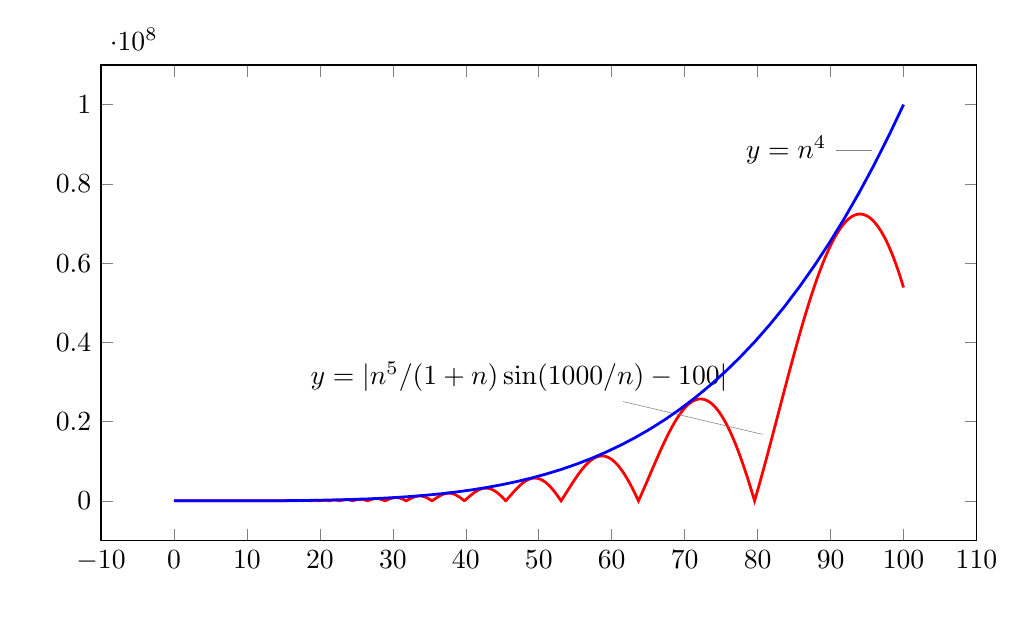
\begin{tikzpicture}[line width=1]
\begin{axis}[width=5in, height=3in,
             scatter/classes={a={mark=*,draw=black}},
             xlabel={\mbox{}},
             xlabel style={name=xlabel}, 
             ylabel={\mbox{}}, 
             legend style={
                at={(xlabel.south)},
                yshift=-1ex,
                anchor=north,
                legend cell align=left,
                },
        ]
]
\addplot[draw=red, line width=1] coordinates {(0.1001,100.0)
(0.2002,100.0)
(0.3003,100.0002)
(0.4004,99.9995)
(0.5005,100.0011)
(0.6006,100.0022)
(0.7007,99.9247)
(0.8008,100.1828)
(0.9009,100.2657)
(1.001,100.0133)
(1.1011,100.1992)
(1.2012,99.9749)
(1.3013,98.4725)
(1.4014,100.9381)
(1.5015,100.0538)
(1.6016,97.0887)
(1.7017,100.8896)
(1.8018,94.0809)
(1.9019,107.8044)
(2.002,99.8583)
(2.1021,112.8617)
(2.2022,83.9634)
(2.3023,85.839)
(2.4024,76.4811)
(2.5025,116.2298)
(2.6026,72.9149)
(2.7027,125.3258)
(2.8028,144.4373)
(2.9029,146.8884)
(3.003,100.5382)
(3.1031,31.9667)
(3.2032,173.8673)
(3.3033,17.1679)
(3.4034,203.329)
(3.5035,48.3478)
(3.6036,13.8306)
(3.7037,126.0836)
(3.8038,239.4049)
(3.9039,283.706)
(4.004,305.6579)
(4.1041,324.2276)
(4.2042,298.3106)
(4.3043,142.2508)
(4.4044,130.5626)
(4.5045,192.7602)
(4.6046,245.1909)
(4.7047,455.4141)
(4.8048,210.2191)
(4.9049,53.9576)
(5.005,598.2596)
(5.1051,407.1111)
(5.2052,383.3936)
(5.3053,103.3283)
(5.4054,149.718)
(5.5055,523.495)
(5.6056,425.5216)
(5.7057,657.1849)
(5.8058,403.4815)
(5.9059,431.2014)
(6.006,95.0801)
(6.1061,373.5935)
(6.2062,1107.0161)
(6.3063,1260.883)
(6.4064,1314.8029)
(6.5065,277.9063)
(6.6066,788.9728)
(6.7067,1847.7589)
(6.8068,1166.3514)
(6.9069,429.0041)
(7.007,2154.8827)
(7.1071,1284.444)
(7.2072,1077.1534)
(7.3073,2562.8448)
(7.4074,134.4053)
(7.5075,2563.0662)
(7.6076,1518.0771)
(7.7077,2613.5606)
(7.8078,2092.9521)
(7.9079,2370.9351)
(8.008,2693.6456)
(8.1081,2889.8701)
(8.2082,2484.5402)
(8.3083,3434.2696)
(8.4084,2050.9941)
(8.5085,4606.7571)
(8.6086,274.2684)
(8.7087,4994.0438)
(8.8088,2131.4163)
(8.9089,4355.5328)
(9.009,5226.074)
(9.1091,983.3496)
(9.2092,6256.1964)
(9.3093,3758.4852)
(9.4094,3728.1648)
(9.5095,7472.594)
(9.6096,3036.0765)
(9.7097,4985.0636)
(9.8098,8192.6014)
(9.9099,3134.1856)
(10.01,5484.942)
(10.1101,9595.8437)
(10.2102,5288.9201)
(10.3103,3902.7213)
(10.4104,10311.2312)
(10.5105,8594.8574)
(10.6106,128.9197)
(10.7107,9402.378)
(10.8108,12407.6204)
(10.9109,6832.4901)
(11.011,3727.6839)
(11.1111,12400.8448)
(11.2112,13579.235)
(11.3113,6340.1162)
(11.4114,5196.6271)
(11.5115,14462.3398)
(11.6116,16217.2099)
(11.7117,9331.249)
(11.8118,2794.3105)
(11.9119,14137.9183)
(12.012,19119.1102)
(12.1121,15229.9293)
(12.2122,4061.6674)
(12.3123,9571.866)
(12.4124,19842.8254)
(12.5125,22386.8464)
(12.6126,16011.7476)
(12.7127,3037.2035)
(12.8128,11730.4846)
(12.9129,22873.5879)
(13.013,26328.4345)
(13.1131,20743.8265)
(13.2132,7828.858)
(13.3133,8328.0032)
(13.4134,22652.4491)
(13.5135,30689.301)
(13.6136,29913.7809)
(13.7137,20391.4333)
(13.8138,4658.9945)
(13.9139,13068.6007)
(14.014,28089.1825)
(14.1141,36453.586)
(14.2142,35934.4824)
(14.3143,26508.1455)
(14.4144,10276.8264)
(14.5145,9099.917)
(14.6146,27291.2811)
(14.7147,40273.5492)
(14.8148,45180.8246)
(14.9149,40860.079)
(15.015,28042.3956)
(15.1151,9129.4627)
(15.2152,12329.9277)
(15.3153,32347.4708)
(15.4154,47240.5164)
(15.5155,54277.3593)
(15.6156,52117.749)
(15.7157,40990.3766)
(15.8158,22599.6637)
(15.9159,200.4889)
(16.016,23894.927)
(16.1161,44868.4877)
(16.2162,59949.4509)
(16.3163,66856.4708)
(16.4164,64492.4454)
(16.5165,53056.3329)
(16.6166,33972.1414)
(16.7167,9659.1518)
(16.8168,16813.9947)
(16.9169,42138.0052)
(17.017,63178.5121)
(17.1171,77347.3166)
(17.2172,82888.5133)
(17.3173,79052.7539)
(17.4174,66148.4122)
(17.5175,45473.3572)
(17.6176,19143.823)
(17.7177,10153.6622)
(17.8178,39455.7205)
(17.9179,65827.7256)
(18.018,86650.28)
(18.1181,99860.1303)
(18.2182,104125.9617)
(18.3183,98947.4895)
(18.4184,84674.4174)
(18.5185,62449.3939)
(18.6186,34085.4339)
(18.7187,1892.9828)
(18.8188,31525.3167)
(18.9189,63493.0585)
(19.019,91473.2682)
(19.1191,113259.9947)
(19.2192,127135.0898)
(19.3193,131980.8007)
(19.4194,127342.9442)
(19.5195,113443.5144)
(19.6196,91145.3152)
(19.7197,61874.3566)
(19.8198,27508.1748)
(19.9199,9760.1684)
(20.02,47571.8779)
(20.1201,83555.4885)
(20.2202,115473.3691)
(20.3203,141353.0837)
(20.4204,159596.6845)
(20.5205,169062.9212)
(20.6206,169119.3738)
(20.7207,159663.5061)
(20.8208,141113.4886)
(20.9209,114371.2546)
(21.021,80761.5679)
(21.1211,41951.8618)
(21.2212,141.7691)
(21.3213,43456.7616)
(21.4214,85888.8439)
(21.5215,125394.0689)
(21.6216,160083.385)
(21.7217,188305.7481)
(21.8218,208716.6351)
(21.9219,220329.7467)
(22.022,222550.6272)
(22.1221,215191.8374)
(22.2222,198470.156)
(22.3223,172987.0251)
(22.4224,139694.0704)
(22.5225,99846.0078)
(22.6226,54943.5889)
(22.7227,6669.4318)
(22.8228,43180.3465)
(22.9229,92765.844)
(23.023,140271.7408)
(23.1231,183971.8826)
(23.2232,222287.9668)
(23.3233,253840.587)
(23.4234,277491.2964)
(23.5235,292374.7655)
(23.6236,297920.5186)
(23.7237,293864.1258)
(23.8238,280248.0903)
(23.9239,257412.9898)
(24.024,225979.7059)
(24.1241,186823.8008)
(24.2242,141043.2658)
(24.3243,89920.988)
(24.4244,34883.3387)
(24.5245,22543.6903)
(24.6246,80779.4108)
(24.7247,138233.0958)
(24.8248,193347.1463)
(24.9249,244637.6684)
(25.025,290731.5119)
(25.1251,330398.9831)
(25.2252,362581.6136)
(25.3253,386414.54)
(25.4254,401243.2202)
(25.5255,406634.3742)
(25.6256,402381.1901)
(25.7257,388502.9758)
(25.8258,365239.5579)
(25.9259,333040.8387)
(26.026,292552.0031)
(26.1261,244594.9425)
(26.2262,190146.5057)
(26.3263,130314.2209)
(26.4264,66310.1468)
(26.5265,576.494)
(26.6266,69007.2594)
(26.7267,137622.4031)
(26.8268,205068.1918)
(26.9269,270023.1049)
(27.027,331222.4554)
(27.1271,387481.0298)
(27.2272,437713.4121)
(27.3273,480951.722)
(27.4274,516360.565)
(27.5275,543249.0585)
(27.6276,561079.8606)
(27.7277,569475.1872)
(27.8278,568219.8621)
(27.9279,557261.49)
(28.028,536707.8931)
(28.1281,506821.9862)
(28.2282,468014.3022)
(28.3283,420833.4028)
(28.4284,365954.4347)
(28.5285,304166.1019)
(28.6286,236356.3357)
(28.7287,163496.949)
(28.8288,86627.5576)
(28.9289,6839.0478)
(29.029,74743.1427)
(29.1291,156975.6732)
(29.2292,238713.6418)
(29.3293,318826.3981)
(29.4294,396212.6293)
(29.5295,469814.5428)
(29.6296,538630.9906)
(29.7297,601729.4082)
(29.8298,658256.4606)
(29.9299,707447.3145)
(30.03,748633.4799)
(30.1301,781249.1821)
(30.2302,804836.2539)
(30.3303,819047.5503)
(30.4304,823648.9121)
(30.5305,818519.7193)
(30.6306,803652.0908)
(30.7307,779148.8008)
(30.8308,745219.9936)
(30.9309,702178.7887)
(31.031,650435.8753)
(31.1311,590493.2034)
(31.2312,522936.8804)
(31.3313,448429.3877)
(31.4314,367701.2316)
(31.5315,281542.1433)
(31.6316,190791.9415)
(31.7317,96331.1678)
(31.8318,928.3975)
(31.9319,100053.2373)
(32.032,200097.5198)
(32.1321,300112.3503)
(32.2322,399154.7684)
(32.3323,496296.4133)
(32.4324,590631.7889)
(32.5325,681286.0651)
(32.6326,767422.3629)
(32.7327,848248.4765)
(32.8328,923022.9952)
(32.9329,991060.7928)
(33.033,1051737.8637)
(33.1331,1104495.489)
(33.2332,1148843.7235)
(33.3333,1184364.2024)
(33.4334,1210712.2714)
(33.5335,1227618.4494)
(33.6336,1234889.2402)
(33.7337,1232407.3119)
(33.8338,1220131.0688)
(33.9339,1198093.6443)
(34.034,1166401.3455)
(34.1341,1125231.5851)
(34.2342,1074830.3359)
(34.3343,1015509.1476)
(34.4344,947641.7672)
(34.5345,871660.4015)
(34.6346,788051.6665)
(34.7347,697352.2652)
(34.8348,600144.4351)
(34.9349,497051.2082)
(35.035,388731.5251)
(35.1351,275875.2418)
(35.2352,159198.0698)
(35.3353,39436.4856)
(35.4354,82657.3532)
(35.5355,206320.6522)
(35.6356,330784.9528)
(35.7357,455281.0023)
(35.8358,579043.4945)
(35.9359,701315.6549)
(36.036,821353.6471)
(36.1361,938430.7798)
(36.2362,1051841.4954)
(36.3363,1160905.1237)
(36.4364,1264969.3876)
(36.5365,1363413.6478)
(36.6366,1455651.8775)
(36.7367,1541135.3603)
(36.8368,1619355.1045)
(36.9369,1689843.9714)
(37.037,1752178.5162)
(37.1371,1805980.5411)
(37.2372,1850918.3627)
(37.3373,1886707.798)
(37.4374,1913112.8727)
(37.5375,1929946.2594)
(37.6376,1937069.4527)
(37.7377,1934392.6891)
(37.8378,1921874.6238)
(37.9379,1899521.7717)
(38.038,1867387.7274)
(38.1381,1825572.173)
(38.2382,1774219.6893)
(38.3383,1713518.3811)
(38.4384,1643698.3321)
(38.5385,1565029.9007)
(38.6386,1477821.8735)
(38.7387,1382419.4883)
(38.8388,1279202.3413)
(38.9389,1168582.1925)
(39.039,1051000.684)
(39.1391,926926.9828)
(39.2392,796855.3637)
(39.3393,661302.7441)
(39.4394,520806.1832)
(39.5395,375920.3597)
(39.6396,227215.0373)
(39.7397,75272.5315)
(39.8398,79314.8119)
(39.9399,235947.1174)
(40.04,394019.4477)
(40.1401,552924.2317)
(40.2402,712053.6422)
(40.3403,870801.9162)
(40.4404,1028567.6105)
(40.5405,1184755.7848)
(40.6406,1338780.1072)
(40.7407,1490064.875)
(40.8408,1638046.9477)
(40.9409,1782177.5856)
(41.041,1921924.1916)
(41.1411,2056771.9522)
(41.2412,2186225.3748)
(41.3413,2309809.7197)
(41.4414,2427072.3244)
(41.5415,2537583.8187)
(41.6416,2640939.2307)
(41.7417,2736758.983)
(41.8418,2824689.7785)
(41.9419,2904405.3773)
(42.042,2975607.2649)
(42.1421,3038025.2135)
(42.2422,3091417.7372)
(42.3423,3135572.4442)
(42.4424,3170306.2866)
(42.5425,3195465.7119)
(42.6426,3210926.7177)
(42.7427,3216594.8133)
(42.8428,3212404.8909)
(42.9429,3198321.0099)
(43.043,3174336.0975)
(43.1431,3140471.5704)
(43.2432,3096776.879)
(43.3433,3043328.9808)
(43.4434,2980231.7445)
(43.5435,2907615.2901)
(43.6436,2825635.2691)
(43.7437,2734472.088)
(43.8438,2634330.0796)
(43.9439,2525436.6271)
(44.044,2408041.243)
(44.1441,2282414.6093)
(44.2442,2148847.5809)
(44.3443,2007650.1572)
(44.4444,1859150.4264)
(44.5445,1703693.4843)
(44.6446,1541640.3338)
(44.7447,1373366.7666)
(44.8448,1199262.2325)
(44.9449,1019728.6981)
(45.045,835179.4996)
(45.1451,646038.1924)
(45.2452,452737.4003)
(45.3453,255717.6676)
(45.4454,55426.3176)
(45.5455,147683.6808)
(45.6456,353154.8356)
(45.7457,560526.2397)
(45.8458,769334.6635)
(45.9459,979115.6291)
(46.046,1189404.464)
(46.1461,1399737.3324)
(46.2462,1609652.243)
(46.3463,1818690.0298)
(46.4464,2026395.3067)
(46.5465,2232317.3927)
(46.6466,2436011.2064)
(46.7467,2637038.1306)
(46.8468,2834966.8429)
(46.9469,3029374.1142)
(47.047,3219845.5723)
(47.1471,3405976.4309)
(47.2472,3587372.1833)
(47.3473,3763649.2597)
(47.4474,3934435.6485)
(47.5475,4099371.481)
(47.6476,4258109.5786)
(47.7477,4410315.9642)
(47.8478,4555670.3354)
(47.9479,4693866.5018)
(48.048,4824612.7851)
(48.1481,4947632.3825)
(48.2482,5062663.6946)
(48.3483,5169460.6167)
(48.4484,5267792.7952)
(48.5485,5357445.8488)
(48.6486,5438221.5556)
(48.7487,5509938.0063)
(48.8488,5572429.7244)
(48.9489,5625547.7539)
(49.049,5669159.7157)
(49.1491,5703149.8324)
(49.2492,5727418.9243)
(49.3493,5741884.375)
(49.4494,5746480.0692)
(49.5495,5741156.3035)
(49.6496,5725879.6702)
(49.7497,5700632.9156)
(49.8498,5665414.7744)
(49.9499,5620239.7795)
(50.0501,5565138.0503)
(50.1502,5500155.0589)
(50.2503,5425351.3754)
(50.3504,5340802.3947)
(50.4505,5246598.0435)
(50.5506,5142842.4708)
(50.6507,5029653.7214)
(50.7508,4907163.3937)
(50.8509,4775516.2837)
(50.951,4634870.0146)
(51.0511,4485394.6548)
(51.1512,4327272.3232)
(51.2513,4160696.7849)
(51.3514,3985873.0369)
(51.4515,3803016.8847)
(51.5516,3612354.5114)
(51.6517,3414122.0401)
(51.7518,3208565.0893)
(51.8519,2995938.3245)
(51.952,2776505.0041)
(52.0521,2550536.5223)
(52.1522,2318311.9495)
(52.2523,2080117.5701)
(52.3524,1836246.4195)
(52.4525,1586997.8204)
(52.5526,1332676.9192)
(52.6527,1073594.2234)
(52.7528,810065.1406)
(52.8529,542409.5193)
(52.953,270951.1924)
(53.0531,3982.4751)
(53.1532,282061.0358)
(53.2533,562951.4043)
(53.3534,846318.2971)
(53.4535,1131824.6667)
(53.5536,1419132.1302)
(53.6537,1707901.3919)
(53.7538,1997792.6579)
(53.8539,2288466.0455)
(53.954,2579581.9834)
(54.0541,2870801.6052)
(54.1542,3161787.1343)
(54.2543,3452202.2602)
(54.3544,3741712.5071)
(54.4545,4029985.592)
(54.5546,4316691.7751)
(54.6547,4601504.1997)
(54.7548,4884099.2232)
(54.8549,5164156.7381)
(54.955,5441360.4828)
(55.0551,5715398.3429)
(55.1552,5985962.6419)
(55.2553,6252750.4217)
(55.3554,6515463.7129)
(55.4555,6773809.7944)
(55.5556,7027501.443)
(55.6557,7276257.1718)
(55.7558,7519801.4585)
(55.8559,7757864.9633)
(55.956,7990184.7359)
(56.0561,8216504.4123)
(56.1562,8436574.4004)
(56.2563,8650152.0566)
(56.3564,8857001.8503)
(56.4565,9056895.5196)
(56.5566,9249612.2156)
(56.6567,9434938.6372)
(56.7568,9612669.1561)
(56.8569,9782605.9309)
(56.957,9944559.0121)
(57.0571,10098346.4377)
(57.1572,10243794.3184)
(57.2573,10380736.9137)
(57.3574,10509016.6993)
(57.4575,10628484.4245)
(57.5576,10738999.1611)
(57.6577,10840428.3436)
(57.7578,10932647.8005)
(57.8579,11015541.7775)
(57.958,11089002.9518)
(58.0581,11152932.4389)
(58.1582,11207239.7917)
(58.2583,11251842.9908)
(58.3584,11286668.4285)
(58.4585,11311650.8849)
(58.5586,11326733.4968)
(58.6587,11331867.7198)
(58.7588,11327013.2838)
(58.8589,11312138.1419)
(58.959,11287218.4127)
(59.0591,11252238.3169)
(59.1592,11207190.1079)
(59.2593,11152073.9963)
(59.3594,11086898.0694)
(59.4595,11011678.2052)
(59.5596,10926437.9813)
(59.6597,10831208.5784)
(59.7598,10726028.6806)
(59.8599,10610944.3692)
(59.96,10486009.0136)
(60.0601,10351283.1581)
(60.1602,10206834.4035)
(60.2603,10052737.2867)
(60.3604,9889073.1557)
(60.4605,9715930.0414)
(60.5606,9533402.5265)
(60.6607,9341591.6117)
(60.7608,9140604.578)
(60.8609,8930554.848)
(60.961,8711561.8436)
(61.0611,8483750.8415)
(61.1612,8247252.8278)
(61.2613,8002204.3491)
(61.3614,7748747.363)
(61.4615,7487029.0866)
(61.5616,7217201.8433)
(61.6617,6939422.9095)
(61.7618,6653854.3585)
(61.8619,6360662.9047)
(61.962,6060019.7467)
(62.0621,5752100.4094)
(62.1622,5437084.5862)
(62.2623,5115155.98)
(62.3624,4786502.1444)
(62.4625,4451314.325)
(62.5626,4109787.3004)
(62.6627,3762119.223)
(62.7628,3408511.4607)
(62.8629,3049168.4383)
(62.963,2684297.4801)
(63.0631,2314108.6523)
(63.1632,1938814.6064)
(63.2633,1558630.4237)
(63.3634,1173773.4598)
(63.4635,784463.1914)
(63.5636,390921.0623)
(63.6637,6629.6672)
(63.7638,407964.072)
(63.8639,812855.7107)
(63.964,1221076.7738)
(64.0641,1632398.2301)
(64.1642,2046589.9716)
(64.2643,2463420.9569)
(64.3644,2882659.3527)
(64.4645,3304072.6739)
(64.5646,3727427.9217)
(64.6647,4152491.7199)
(64.7648,4579030.4493)
(64.8649,5006810.3803)
(64.965,5435597.8034)
(65.0651,5865159.1577)
(65.1652,6295261.1573)
(65.2653,6725670.9156)
(65.3654,7156156.0675)
(65.4655,7586484.8893)
(65.5656,8016426.4167)
(65.6657,8445750.56)
(65.7658,8874228.2178)
(65.8659,9301631.3876)
(65.966,9727733.2747)
(66.0661,10152308.3984)
(66.1662,10575132.6964)
(66.2663,10995983.6257)
(66.3664,11414640.2625)
(66.4665,11830883.3989)
(66.5666,12244495.6371)
(66.6667,12655261.4821)
(66.7668,13062967.4306)
(66.8669,13467402.0587)
(66.967,13868356.1067)
(67.0671,14265622.5615)
(67.1672,14658996.7364)
(67.2673,15048276.3492)
(67.3674,15433261.5966)
(67.4675,15813755.2277)
(67.5676,16189562.6141)
(67.6677,16560491.818)
(67.7678,16926353.6576)
(67.8679,17286961.7707)
(67.968,17642132.6753)
(68.0681,17991685.8284)
(68.1682,18335443.6823)
(68.2683,18673231.7384)
(68.3684,19004878.5988)
(68.4685,19330216.0161)
(68.5686,19649078.94)
(68.6687,19961305.5627)
(68.7688,20266737.3612)
(68.8689,20565219.1381)
(68.969,20856599.0599)
(69.0691,21140728.6931)
(69.1692,21417463.0382)
(69.2693,21686660.5622)
(69.3694,21948183.2278)
(69.4695,22201896.5219)
(69.5696,22447669.4809)
(69.6697,22685374.7151)
(69.7698,22914888.4303)
(69.8699,23136090.4478)
(69.97,23348864.2227)
(70.0701,23553096.8596)
(70.1702,23748679.1275)
(70.2703,23935505.4719)
(70.3704,24113474.0257)
(70.4705,24282486.6182)
(70.5706,24442448.7824)
(70.6707,24593269.7603)
(70.7708,24734862.5069)
(70.8709,24867143.6925)
(70.971,24990033.7034)
(71.0711,25103456.6408)
(71.1712,25207340.3181)
(71.2713,25301616.2575)
(71.3714,25386219.684)
(71.4715,25461089.5187)
(71.5716,25526168.3704)
(71.6717,25581402.5258)
(71.7718,25626741.9385)
(71.8719,25662140.2167)
(71.972,25687554.6091)
(72.0721,25702945.9903)
(72.1722,25708278.8446)
(72.2723,25703521.2482)
(72.3724,25688644.8513)
(72.4725,25663624.8576)
(72.5726,25628440.0041)
(72.6727,25583072.5391)
(72.7728,25527508.199)
(72.8729,25461736.1846)
(72.973,25385749.1361)
(73.0731,25299543.1071)
(73.1732,25203117.538)
(73.2733,25096475.2279)
(73.3734,24979622.3065)
(73.4735,24852568.2043)
(73.5736,24715325.6224)
(73.6737,24567910.5016)
(73.7738,24410341.9907)
(73.8739,24242642.4135)
(73.974,24064837.2362)
(74.0741,23876955.033)
(74.1742,23679027.4519)
(74.2743,23471089.1794)
(74.3744,23253177.9047)
(74.4745,23025334.2834)
(74.5746,22787601.9006)
(74.6747,22540027.2337)
(74.7748,22282659.6141)
(74.8749,22015551.1893)
(74.975,21738756.8835)
(75.0751,21452334.3592)
(75.1752,21156343.9765)
(75.2753,20850848.7542)
(75.3754,20535914.3285)
(75.4755,20211608.9128)
(75.5756,19878003.2565)
(75.6757,19535170.6038)
(75.7758,19183186.652)
(75.8759,18822129.5096)
(75.976,18452079.6547)
(76.0761,18073119.892)
(76.1762,17685335.3109)
(76.2763,17288813.2429)
(76.3764,16883643.2182)
(76.4765,16469916.9237)
(76.5766,16047728.1591)
(76.6767,15617172.7943)
(76.7768,15178348.7263)
(76.8769,14731355.8355)
(76.977,14276295.9424)
(77.0771,13813272.7649)
(77.1772,13342391.8742)
(77.2773,12863760.6519)
(77.3774,12377488.2465)
(77.4775,11883685.53)
(77.5776,11382465.0549)
(77.6777,10873941.0109)
(77.7778,10358229.1817)
(77.8779,9835446.902)
(77.978,9305713.0147)
(78.0781,8769147.8278)
(78.1782,8225873.0722)
(78.2783,7676011.8586)
(78.3784,7119688.6353)
(78.4785,6557029.1463)
(78.5786,5988160.3887)
(78.6787,5413210.5711)
(78.7788,4832309.0719)
(78.8789,4245586.398)
(78.979,3653174.1431)
(79.0791,3055204.9469)
(79.1792,2451812.4545)
(79.2793,1843131.2754)
(79.3794,1229296.9437)
(79.4795,610445.8774)
(79.5796,13284.6606)
(79.6797,641756.6028)
(79.7798,1274831.1156)
(79.8799,1912368.6387)
(79.98,2554228.9236)
(80.0801,3200271.072)
(80.1802,3850353.5736)
(80.2803,4504334.344)
(80.3804,5162070.762)
(80.4805,5823419.7066)
(80.5806,6488237.5938)
(80.6807,7156380.4129)
(80.7808,7827703.7625)
(80.8809,8502062.8863)
(80.981,9179312.7082)
(81.0811,9859307.8673)
(81.1812,10541902.7529)
(81.2813,11226951.538)
(81.3814,11914308.2137)
(81.4815,12603826.6224)
(81.5816,13295360.4911)
(81.6817,13988763.4639)
(81.7818,14683889.1345)
(81.8819,15380591.0782)
(81.982,16078722.8829)
(82.0821,16778138.1812)
(82.1822,17478690.6802)
(82.2823,18180234.1926)
(82.3824,18882622.6663)
(82.4825,19585710.2138)
(82.5826,20289351.1421)
(82.6827,20993399.9804)
(82.7828,21697711.5095)
(82.8829,22402140.7891)
(82.983,23106543.1854)
(83.0831,23810774.3985)
(83.1832,24514690.4891)
(83.2833,25218147.9046)
(83.3834,25921003.5051)
(83.4835,26623114.5891)
(83.5836,27324338.9184)
(83.6837,28024534.7427)
(83.7838,28723560.8243)
(83.8839,29421276.4616)
(83.984,30117541.5126)
(84.0841,30812216.4181)
(84.1842,31505162.2245)
(84.2843,32196240.6056)
(84.3844,32885313.8849)
(84.4845,33572245.0567)
(84.5846,34256897.8075)
(84.6847,34939136.5362)
(84.7848,35618826.375)
(84.8849,36295833.2086)
(84.985,36970023.6938)
(85.0851,37641265.2789)
(85.1852,38309426.222)
(85.2853,38974375.6095)
(85.3854,39635983.3738)
(85.4855,40294120.311)
(85.5856,40948658.0978)
(85.6857,41599469.3084)
(85.7858,42246427.4308)
(85.8859,42889406.8828)
(85.986,43528283.0273)
(86.0861,44162932.1881)
(86.1862,44793231.6643)
(86.2863,45419059.7448)
(86.3864,46040295.7226)
(86.4865,46656819.9084)
(86.5866,47268513.6443)
(86.6867,47875259.3161)
(86.7868,48476940.3669)
(86.8869,49073441.3088)
(86.987,49664647.7348)
(87.0871,50250446.3311)
(87.1872,50830724.8874)
(87.2873,51405372.3089)
(87.3874,51974278.6259)
(87.4875,52537335.0048)
(87.5876,53094433.7575)
(87.6877,53645468.3515)
(87.7878,54190333.4185)
(87.8879,54728924.7642)
(87.988,55261139.3761)
(88.0881,55786875.4324)
(88.1882,56306032.3095)
(88.2883,56818510.5902)
(88.3884,57324212.0707)
(88.4885,57823039.7678)
(88.5886,58314897.9256)
(88.6887,58799692.0219)
(88.7888,59277328.7749)
(88.8889,59747716.1482)
(88.989,60210763.3571)
(89.0891,60666380.8737)
(89.1892,61114480.4317)
(89.2893,61554975.0317)
(89.3894,61987778.9449)
(89.4895,62412807.718)
(89.5896,62829978.1769)
(89.6897,63239208.4301)
(89.7898,63640417.8726)
(89.8899,64033527.1885)
(89.99,64418458.3545)
(90.0901,64795134.6421)
(90.1902,65163480.62)
(90.2903,65523422.1565)
(90.3904,65874886.4214)
(90.4905,66217801.8872)
(90.5906,66552098.3314)
(90.6907,66877706.8368)
(90.7908,67194559.793)
(90.8909,67502590.897)
(90.991,67801735.1539)
(91.0911,68091928.877)
(91.1912,68373109.6878)
(91.2913,68645216.5164)
(91.3914,68908189.6005)
(91.4915,69161970.4853)
(91.5916,69406502.023)
(91.6917,69641728.371)
(91.7918,69867594.9917)
(91.8919,70084048.6508)
(91.992,70291037.4156)
(92.0921,70488510.6536)
(92.1922,70676419.0307)
(92.2923,70854714.5088)
(92.3924,71023350.3438)
(92.4925,71182281.0831)
(92.5926,71331462.5632)
(92.6927,71470851.9066)
(92.7928,71600407.5194)
(92.8929,71720089.0877)
(92.993,71829857.5748)
(93.0931,71929675.2176)
(93.1932,72019505.523)
(93.2933,72099313.2644)
(93.3934,72169064.4777)
(93.4935,72228726.4577)
(93.5936,72278267.7533)
(93.6937,72317658.1638)
(93.7938,72346868.7344)
(93.8939,72365871.7515)
(93.994,72374640.7384)
(94.0941,72373150.4499)
(94.1942,72361376.8682)
(94.2943,72339297.1971)
(94.3944,72306889.8574)
(94.4945,72264134.4814)
(94.5946,72211011.9075)
(94.6947,72147504.175)
(94.7948,72073594.5181)
(94.8949,71989267.3603)
(94.995,71894508.3088)
(95.0951,71789304.1486)
(95.1952,71673642.8362)
(95.2953,71547513.4936)
(95.3954,71410906.4023)
(95.4955,71263812.9968)
(95.5956,71106225.8585)
(95.6957,70938138.7088)
(95.7958,70759546.403)
(95.8959,70570444.9232)
(95.996,70370831.3723)
(96.0961,70160703.9664)
(96.1962,69940062.0285)
(96.2963,69708905.9813)
(96.3964,69467237.3405)
(96.4965,69215058.7072)
(96.5966,68952373.7614)
(96.6967,68679187.2542)
(96.7968,68395505.0011)
(96.8969,68101333.874)
(96.997,67796681.7947)
(97.0971,67481557.7265)
(97.1972,67155971.6675)
(97.2973,66819934.6426)
(97.3974,66473458.6961)
(97.4975,66116556.8838)
(97.5976,65749243.2657)
(97.6977,65371532.8979)
(97.7978,64983441.8252)
(97.8979,64584987.073)
(97.998,64176186.6392)
(98.0981,63757059.4871)
(98.1982,63327625.5366)
(98.2983,62887905.6567)
(98.3984,62437921.6576)
(98.4985,61977696.2822)
(98.5986,61507253.1986)
(98.6987,61026616.9914)
(98.7988,60535813.1543)
(98.8989,60034868.0814)
(98.999,59523809.0592)
(99.0991,59002664.2584)
(99.1992,58471462.7261)
(99.2993,57930234.3768)
(99.3994,57379009.9849)
(99.4995,56817821.1759)
(99.5996,56246700.4187)
(99.6997,55665681.0167)
(99.7998,55074797.1001)
(99.8999,54474083.617)
(100.0,53863576.3257)};\node[pin=above left:{$y=|n^5/(1+n) \sin(1000/n) - 100|$}] at (axis cs:82,16204527.16254407) {};\addplot[draw=blue, line width=1] coordinates {(0.0,0.0)
(2.0408,17.3467)
(4.0816,277.5464)
(6.1224,1405.0789)
(8.1633,4440.7431)
(10.2041,10841.6578)
(12.2449,22481.2617)
(14.2857,41649.3128)
(16.3265,71051.8889)
(18.3673,113811.3874)
(20.4082,173466.5256)
(22.449,253972.3401)
(24.4898,359700.1874)
(26.5306,495437.7436)
(28.5714,666389.0046)
(30.6122,878174.2856)
(32.6531,1136830.2219)
(34.6939,1448809.7681)
(36.7347,1820982.1987)
(38.7755,2260633.1077)
(40.8163,2775464.4089)
(42.8571,3373594.3357)
(44.898,4063557.4411)
(46.9388,4854304.5979)
(48.9796,5755202.9983)
(51.0204,6776036.1546)
(53.0612,7927003.8983)
(55.102,9218722.3809)
(57.1429,10662224.0733)
(59.1837,12268957.7663)
(61.2245,14050788.5702)
(63.2653,16019997.9149)
(65.3061,18189283.5503)
(67.3469,20571759.5456)
(69.3878,23180956.2897)
(71.4286,26030820.4915)
(73.4694,29135715.1791)
(75.5102,32510419.7005)
(77.551,36170129.7235)
(79.5918,40130457.2352)
(81.6327,44407430.5427)
(83.6735,49017494.2726)
(85.7143,53977509.3711)
(87.7551,59304753.1042)
(89.7959,65016919.0576)
(91.8367,71132117.1364)
(93.8776,77668873.5656)
(95.9184,84646130.8899)
(97.9592,92083247.9733)
(100.0,100000000.0)};\node[pin=left:{$y=n^4$}] at (axis cs:97,88529281) {};
\end{axis}\end{tikzpicture}\end{center}

%-*-latex-*-

\begin{center}
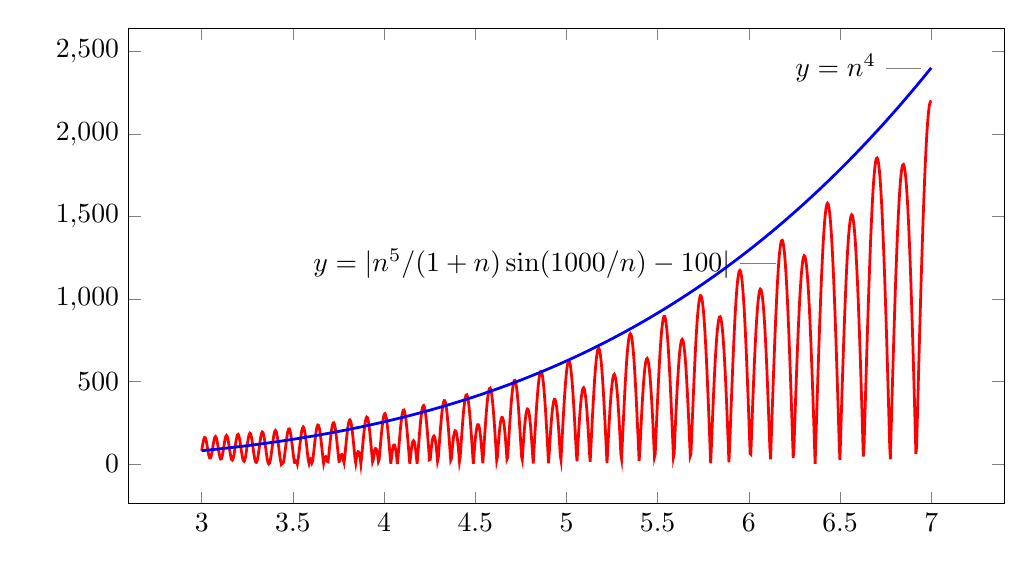
\begin{tikzpicture}[line width=1]
\begin{axis}[width=5in, height=3in,
             scatter/classes={a={mark=*,draw=black}},
             xlabel={\mbox{}},
             xlabel style={name=xlabel}, 
             ylabel={\mbox{}}, 
             legend style={
                at={(xlabel.south)},
                yshift=-1ex,
                anchor=north,
                legend cell align=left,
                },
        ]
]
\addplot[draw=red, line width=1] coordinates {(3.0,80.6301)
(3.004,107.3008)
(3.008,132.7879)
(3.012,152.1556)
(3.016,161.6538)
(3.02,159.4284)
(3.024,145.8614)
(3.028,123.483)
(3.032,96.4803)
(3.036,69.9005)
(3.04,48.7036)
(3.044,36.8426)
(3.048,36.5403)
(3.0521,47.8931)
(3.0561,68.8678)
(3.0601,95.6852)
(3.0641,123.5163)
(3.0681,147.3573)
(3.0721,162.9271)
(3.0761,167.4241)
(3.0801,160.0131)
(3.0841,141.9589)
(3.0881,116.3902)
(3.0921,87.7417)
(3.0961,60.975)
(3.1001,40.7188)
(3.1041,30.4755)
(3.1081,32.0305)
(3.1121,45.16)
(3.1161,67.6821)
(3.1201,95.8374)
(3.1241,124.9296)
(3.1281,150.1137)
(3.1321,167.2007)
(3.1361,173.3442)
(3.1401,167.4988)
(3.1441,150.5785)
(3.1481,125.2953)
(3.1522,95.7087)
(3.1562,66.5638)
(3.1602,42.5272)
(3.1642,27.4442)
(3.1682,23.7351)
(3.1722,32.0227)
(3.1762,51.0469)
(3.1802,77.8734)
(3.1842,108.361)
(3.1882,137.8095)
(3.1922,161.686)
(3.1962,176.3181)
(3.2002,179.4469)
(3.2042,170.5604)
(3.2082,150.9589)
(3.2122,123.5483)
(3.2162,92.3955)
(3.2202,62.1167)
(3.2242,37.1912)
(3.2282,21.3035)
(3.2322,16.809)
(3.2362,24.3995)
(3.2402,43.0139)
(3.2442,70.0026)
(3.2482,101.5182)
(3.2523,133.0731)
(3.2563,160.1813)
(3.2603,178.9934)
(3.2643,186.8342)
(3.2683,182.5699)
(3.2723,166.7562)
(3.2763,141.5504)
(3.2803,110.4031)
(3.2843,77.5755)
(3.2883,47.5516)
(3.2923,24.4266)
(3.2963,11.3545)
(3.3003,10.1293)
(3.3043,20.9528)
(3.3083,42.4179)
(3.3123,71.7064)
(3.3163,104.9699)
(3.3203,137.8434)
(3.3243,166.0202)
(3.3283,185.8126)
(3.3323,194.6268)
(3.3363,191.2905)
(3.3403,176.1945)
(3.3443,151.2328)
(3.3483,119.5522)
(3.3524,85.145)
(3.3564,52.3413)
(3.3604,25.2625)
(3.3644,7.3084)
(3.3684,0.739)
(3.3724,6.4023)
(3.3764,23.6384)
(3.3804,50.3701)
(3.3844,83.3656)
(3.3884,118.6375)
(3.3924,151.9301)
(3.3964,179.2324)
(3.4004,197.2574)
(3.4044,203.8288)
(3.4084,198.1324)
(3.4124,180.8035)
(3.4164,153.8434)
(3.4204,120.3766)
(3.4244,84.28)
(3.4284,49.7289)
(3.4324,20.7136)
(3.4364,0.5824)
(3.4404,8.3373)
(3.4444,4.9971)
(3.4484,10.2613)
(3.4525,35.7536)
(3.4565,68.6498)
(3.4605,105.2979)
(3.4645,141.6345)
(3.4685,173.6374)
(3.4725,197.7682)
(3.4765,211.3574)
(3.4805,212.8906)
(3.4845,202.1656)
(3.4885,180.3064)
(3.4925,149.634)
(3.4965,113.4102)
(3.5005,75.4839)
(3.5045,39.8785)
(3.5085,10.3655)
(3.5125,9.9307)
(3.5165,18.8568)
(3.5205,15.4484)
(3.5245,0.0237)
(3.5285,25.8576)
(3.5325,59.5624)
(3.5365,97.6605)
(3.5405,136.2791)
(3.5445,171.4987)
(3.5485,199.7499)
(3.5526,218.1699)
(3.5566,224.8853)
(3.5606,219.1929)
(3.5646,201.6223)
(3.5686,173.8762)
(3.5726,138.6559)
(3.5766,99.3902)
(3.5806,59.8971)
(3.5846,24.0105)
(3.5886,4.7904)
(3.5926,23.7139)
(3.5966,30.9188)
(3.6006,25.6848)
(3.6046,8.4739)
(3.6086,19.1203)
(3.6126,54.5295)
(3.6166,94.4571)
(3.6206,135.1902)
(3.6246,172.9471)
(3.6286,204.2271)
(3.6326,226.1318)
(3.6366,236.6266)
(3.6406,234.7218)
(3.6446,220.556)
(3.6486,195.377)
(3.6527,161.4229)
(3.6567,121.715)
(3.6607,79.7841)
(3.6647,39.3526)
(3.6687,4.0047)
(3.6727,23.1296)
(3.6767,39.6459)
(3.6807,44.0716)
(3.6847,35.9883)
(3.6887,16.0623)
(3.6927,14.0198)
(3.6967,51.7017)
(3.7007,93.7812)
(3.7047,136.6867)
(3.7087,176.782)
(3.7127,210.6742)
(3.7167,235.497)
(3.7207,249.1478)
(3.7247,250.4585)
(3.7287,239.2871)
(3.7327,216.523)
(3.7367,184.0086)
(3.7407,144.3819)
(3.7447,100.8571)
(3.7487,56.9603)
(3.7528,16.2418)
(3.7568,18.0094)
(3.7608,43.0283)
(3.7648,56.7919)
(3.7688,58.1751)
(3.7728,47.0357)
(3.7768,24.2188)
(3.7808,8.5143)
(3.7848,48.6298)
(3.7888,93.0229)
(3.7928,138.2618)
(3.7968,180.8549)
(3.8008,217.5193)
(3.8048,245.4316)
(3.8088,262.4398)
(3.8128,267.2237)
(3.8168,259.3893)
(3.8208,239.4936)
(3.8248,208.9974)
(3.8288,170.1507)
(3.8328,125.8212)
(3.8368,79.2783)
(3.8408,33.9493)
(3.8448,6.8327)
(3.8488,40.0725)
(3.8529,63.3289)
(3.8569,74.8889)
(3.8609,73.8868)
(3.8649,60.3624)
(3.8689,35.2526)
(3.8729,0.3194)
(3.8769,41.9796)
(3.8809,88.6695)
(3.8849,136.4703)
(3.8889,182.0294)
(3.8929,222.1557)
(3.8969,254.0415)
(3.9009,275.4548)
(3.9049,284.8899)
(3.9089,281.6676)
(3.9129,265.9763)
(3.9169,238.8548)
(3.9209,202.117)
(3.9249,158.2243)
(3.9289,110.1168)
(3.9329,61.0127)
(3.9369,14.1921)
(3.9409,27.222)
(3.9449,60.47)
(3.9489,83.3356)
(3.953,94.2887)
(3.957,92.582)
(3.961,78.295)
(3.965,52.3248)
(3.969,16.3231)
(3.973,27.4144)
(3.977,76.0987)
(3.981,126.6288)
(3.985,175.7909)
(3.989,220.4628)
(3.993,257.8109)
(3.997,285.4666)
(4.001,301.6723)
(4.005,305.388)
(4.009,296.3518)
(4.013,275.0921)
(4.017,242.8903)
(4.021,201.6982)
(4.025,154.0149)
(4.029,102.7313)
(4.033,50.9527)
(4.037,1.8094)
(4.041,41.7316)
(4.045,77.044)
(4.049,101.9971)
(4.0531,115.0802)
(4.0571,115.4885)
(4.0611,103.1673)
(4.0651,78.8105)
(4.0691,43.8164)
(4.0731,0.2022)
(4.0771,49.5171)
(4.0811,102.4763)
(4.0851,155.6278)
(4.0891,205.9177)
(4.0931,250.46)
(4.0971,286.7012)
(4.1011,312.5629)
(4.1051,326.5568)
(4.1091,327.8659)
(4.1131,316.3864)
(4.1171,292.7298)
(4.1211,258.1848)
(4.1251,214.6425)
(4.1291,164.4885)
(4.1331,110.4688)
(4.1371,55.5373)
(4.1411,2.6934)
(4.1451,45.1816)
(4.1491,85.4802)
(4.1532,116.0076)
(4.1572,135.0984)
(4.1612,141.7023)
(4.1652,135.4373)
(4.1692,116.6064)
(4.1732,86.1779)
(4.1772,45.7307)
(4.1812,2.6317)
(4.1852,56.3946)
(4.1892,112.765)
(4.1932,168.8185)
(4.1972,221.6516)
(4.2012,268.5311)
(4.2052,307.0337)
(4.2092,335.1686)
(4.2132,351.4767)
(4.2172,355.102)
(4.2212,345.8315)
(4.2252,324.1029)
(4.2292,290.979)
(4.2332,248.0916)
(4.2372,197.5565)
(4.2412,141.8663)
(4.2452,83.7654)
(4.2492,26.1125)
(4.2533,28.2595)
(4.2573,76.6825)
(4.2613,116.7823)
(4.2653,146.5924)
(4.2693,164.6468)
(4.2733,170.0483)
(4.2773,162.5089)
(4.2813,142.3597)
(4.2853,110.5325)
(4.2893,68.5123)
(4.2933,18.2642)
(4.2973,37.8619)
(4.3013,97.2434)
(4.3053,157.1092)
(4.3093,214.6698)
(4.3133,267.2465)
(4.3173,312.3953)
(4.3213,348.0182)
(4.3253,372.4574)
(4.3293,384.5695)
(4.3333,383.7746)
(4.3373,370.0799)
(4.3413,344.0763)
(4.3453,306.9088)
(4.3493,260.2224)
(4.3534,206.0855)
(4.3574,146.896)
(4.3614,85.2727)
(4.3654,23.9383)
(4.3694,34.4011)
(4.3734,87.1747)
(4.3774,132.0594)
(4.3814,167.0793)
(4.3854,190.6904)
(4.3894,201.8448)
(4.3934,200.0335)
(4.3974,185.306)
(4.4014,158.2648)
(4.4054,120.037)
(4.4094,72.224)
(4.4134,16.8312)
(4.4174,43.8192)
(4.4214,107.1869)
(4.4254,170.6214)
(4.4294,231.473)
(4.4334,287.2037)
(4.4374,335.4909)
(4.4414,374.3232)
(4.4454,402.0813)
(4.4494,417.6022)
(4.4535,420.225)
(4.4575,409.8148)
(4.4615,386.7659)
(4.4655,351.9832)
(4.4695,306.8427)
(4.4735,253.1347)
(4.4775,192.9894)
(4.4815,128.7909)
(4.4855,63.0805)
(4.4895,1.5438)
(4.4935,62.5309)
(4.4975,117.476)
(4.5015,164.2142)
(4.5055,200.9042)
(4.5095,226.0977)
(4.5135,238.7939)
(4.5175,238.4759)
(4.5215,225.1283)
(4.5255,199.2349)
(4.5295,161.7584)
(4.5335,114.1009)
(4.5375,58.0486)
(4.5415,4.2974)
(4.5455,70.6018)
(4.5495,138.3842)
(4.5536,205.1122)
(4.5576,268.2964)
(4.5616,325.5824)
(4.5656,374.8375)
(4.5696,414.2278)
(4.5736,442.285)
(4.5776,457.9574)
(4.5816,460.6472)
(4.5856,450.2291)
(4.5896,427.0534)
(4.5936,391.9305)
(4.5976,346.0997)
(4.6016,291.1825)
(4.6056,229.1229)
(4.6096,162.1169)
(4.6136,92.5325)
(4.6176,22.8261)
(4.6216,44.5454)
(4.6256,107.2101)
(4.6296,162.9645)
(4.6336,209.8491)
(4.6376,246.2153)
(4.6416,270.7814)
(4.6456,282.6747)
(4.6496,281.4598)
(4.6537,267.1514)
(4.6577,240.2115)
(4.6617,201.5317)
(4.6657,152.4008)
(4.6697,94.4591)
(4.6737,29.642)
(4.6777,39.8873)
(4.6817,111.8104)
(4.6857,183.7325)
(4.6897,253.2619)
(4.6937,318.0896)
(4.6977,376.0649)
(4.7017,425.2658)
(4.7057,464.0603)
(4.7097,491.1593)
(4.7137,505.6559)
(4.7177,507.054)
(4.7217,495.2818)
(4.7257,470.6922)
(4.7297,434.0498)
(4.7337,386.504)
(4.7377,329.5507)
(4.7417,264.9831)
(4.7457,194.8333)
(4.7497,121.3072)
(4.7538,46.7139)
(4.7578,26.6072)
(4.7618,96.3595)
(4.7658,160.3609)
(4.7698,216.6108)
(4.7738,263.3515)
(4.7778,299.1212)
(4.7818,322.7975)
(4.7858,333.6301)
(4.7898,331.2626)
(4.7938,315.7407)
(4.7978,287.5096)
(4.8018,247.3981)
(4.8058,196.5923)
(4.8098,136.5981)
(4.8138,69.1945)
(4.8178,3.6207)
(4.8218,79.6913)
(4.8258,156.7676)
(4.8298,232.573)
(4.8338,304.8715)
(4.8378,371.5331)
(4.8418,430.5955)
(4.8458,480.3208)
(4.8498,519.2448)
(4.8539,546.2183)
(4.8579,560.4387)
(4.8619,561.4716)
(4.8659,549.2617)
(4.8699,524.1322)
(4.8739,486.7744)
(4.8779,438.226)
(4.8819,379.84)
(4.8859,313.2456)
(4.8899,240.3006)
(4.8939,163.0383)
(4.8979,83.6102)
(4.9019,4.225)
(4.9059,72.9125)
(4.9099,145.6627)
(4.9139,212.0099)
(4.9179,270.1171)
(4.9219,318.3756)
(4.9259,355.4477)
(4.9299,380.3024)
(4.9339,392.2414)
(4.9379,390.9169)
(4.9419,376.339)
(4.9459,348.8744)
(4.9499,309.2342)
(4.954,258.4539)
(4.958,197.8643)
(4.962,129.0545)
(4.966,53.8291)
(4.97,25.8406)
(4.974,107.8692)
(4.978,190.112)
(4.982,270.4218)
(4.986,346.7043)
(4.99,416.9725)
(4.994,479.3976)
(4.998,532.3553)
(5.002,574.4666)
(5.006,604.6323)
(5.01,622.0596)
(5.014,626.2807)
(5.018,617.1636)
(5.022,594.9139)
(5.026,560.0677)
(5.03,513.4771)
(5.034,456.2872)
(5.038,389.9063)
(5.042,315.9695)
(5.046,236.2975)
(5.0501,152.8501)
(5.0541,67.678)
(5.0581,17.1287)
(5.0621,99.4912)
(5.0661,177.3934)
(5.0701,248.9302)
(5.0741,312.3535)
(5.0781,366.1138)
(5.0821,408.8964)
(5.0861,439.6524)
(5.0901,457.6224)
(5.0941,462.3533)
(5.0981,453.7079)
(5.1021,431.8668)
(5.1061,397.3224)
(5.1101,350.8664)
(5.1141,293.5694)
(5.1181,226.7549)
(5.1221,151.9669)
(5.1261,70.9334)
(5.1301,14.4748)
(5.1341,102.2881)
(5.1381,190.484)
(5.1421,277.0336)
(5.1461,359.9484)
(5.1502,437.3256)
(5.1542,507.391)
(5.1582,568.539)
(5.1622,619.3678)
(5.1662,658.7105)
(5.1702,685.6604)
(5.1742,699.5899)
(5.1782,700.1637)
(5.1822,687.3446)
(5.1862,661.3935)
(5.1902,622.8619)
(5.1942,572.5787)
(5.1982,511.6307)
(5.2022,441.3373)
(5.2062,363.2211)
(5.2102,278.9736)
(5.2142,190.4173)
(5.2182,99.4661)
(5.2222,8.0833)
(5.2262,81.7613)
(5.2302,168.1331)
(5.2342,249.1744)
(5.2382,323.144)
(5.2422,388.4533)
(5.2462,443.6996)
(5.2503,487.6951)
(5.2543,519.4909)
(5.2583,538.3962)
(5.2623,543.9911)
(5.2663,536.1349)
(5.2703,514.9676)
(5.2743,480.9054)
(5.2783,434.6315)
(5.2823,377.0805)
(5.2863,309.4181)
(5.2903,233.0162)
(5.2943,149.4239)
(5.2983,60.3353)
(5.3023,32.4461)
(5.3063,127.0437)
(5.3103,221.5468)
(5.3143,314.049)
(5.3183,402.6863)
(5.3223,485.6746)
(5.3263,561.345)
(5.3303,628.1766)
(5.3343,684.8256)
(5.3383,730.152)
(5.3423,763.2405)
(5.3463,783.4182)
(5.3504,790.2662)
(5.3544,783.6271)
(5.3584,763.607)
(5.3624,730.572)
(5.3664,685.1404)
(5.3704,628.1693)
(5.3744,560.7372)
(5.3784,484.1227)
(5.3824,399.7785)
(5.3864,309.3033)
(5.3904,214.4107)
(5.3944,116.8961)
(5.3984,18.6024)
(5.4024,78.6153)
(5.4064,172.9241)
(5.4104,262.5482)
(5.4144,345.8017)
(5.4184,421.1195)
(5.4224,487.0862)
(5.4264,542.4616)
(5.4304,586.2028)
(5.4344,617.483)
(5.4384,635.7055)
(5.4424,640.5136)
(5.4464,631.7963)
(5.4505,609.6895)
(5.4545,574.5721)
(5.4585,527.0582)
(5.4625,467.9853)
(5.4665,398.3981)
(5.4705,319.5288)
(5.4745,232.7744)
(5.4785,139.6709)
(5.4825,41.8657)
(5.4865,58.9125)
(5.4905,160.8845)
(5.4945,262.2521)
(5.4985,361.23)
(5.5025,456.077)
(5.5065,545.1262)
(5.5105,626.8139)
(5.5145,699.7064)
(5.5185,762.5242)
(5.5225,814.1639)
(5.5265,853.7157)
(5.5305,880.4791)
(5.5345,893.9736)
(5.5385,893.9461)
(5.5425,880.3743)
(5.5465,853.4663)
(5.5506,813.6557)
(5.5546,761.5938)
(5.5586,698.1374)
(5.5626,624.334)
(5.5666,541.403)
(5.5706,450.7146)
(5.5746,353.7671)
(5.5786,252.1604)
(5.5826,147.5701)
(5.5866,41.7187)
(5.5906,63.6522)
(5.5946,166.8115)
(5.5986,266.0659)
(5.6026,359.7881)
(5.6066,446.4429)
(5.6106,524.6114)
(5.6146,593.014)
(5.6186,650.5303)
(5.6226,696.2161)
(5.6266,729.3187)
(5.6306,749.2872)
(5.6346,755.7814)
(5.6386,748.6756)
(5.6426,728.0601)
(5.6466,694.2391)
(5.6507,647.7245)
(5.6547,589.2274)
(5.6587,519.6462)
(5.6627,440.0514)
(5.6667,351.6688)
(5.6707,255.8589)
(5.6747,154.0964)
(5.6787,47.946)
(5.6827,60.9617)
(5.6867,170.9557)
(5.6907,280.3501)
(5.6947,387.4704)
(5.6987,490.6786)
(5.7027,588.3982)
(5.7067,679.1377)
(5.7107,761.5133)
(5.7147,834.2685)
(5.7187,896.2932)
(5.7227,946.6396)
(5.7267,984.5356)
(5.7307,1009.3957)
(5.7347,1020.829)
(5.7387,1018.6442)
(5.7427,1002.8516)
(5.7467,973.6622)
(5.7508,931.4838)
(5.7548,876.9142)
(5.7588,810.7319)
(5.7628,733.8837)
(5.7668,647.4703)
(5.7708,552.7303)
(5.7748,451.0207)
(5.7788,343.798)
(5.7828,232.596)
(5.7868,119.0038)
(5.7908,4.643)
(5.7948,108.8559)
(5.7988,219.8765)
(5.8028,326.8394)
(5.8068,428.2245)
(5.8108,522.5921)
(5.8148,608.6031)
(5.8188,685.0368)
(5.8228,750.8085)
(5.8268,804.983)
(5.8308,846.788)
(5.8348,875.6234)
(5.8388,891.0696)
(5.8428,892.8921)
(5.8468,881.0443)
(5.8509,855.6671)
(5.8549,817.0868)
(5.8589,765.8092)
(5.8629,702.5126)
(5.8669,628.0376)
(5.8709,543.3754)
(5.8749,449.6532)
(5.8789,348.1193)
(5.8829,240.1254)
(5.8869,127.108)
(5.8909,10.5691)
(5.8949,107.9439)
(5.8989,226.8594)
(5.9029,344.6023)
(5.9069,459.6145)
(5.9109,570.376)
(5.9149,675.4243)
(5.9189,773.3733)
(5.9229,862.9314)
(5.9269,942.9179)
(5.9309,1012.2779)
(5.9349,1070.0953)
(5.9389,1115.6044)
(5.9429,1148.1992)
(5.9469,1167.4403)
(5.951,1173.0601)
(5.955,1164.9656)
(5.959,1143.239)
(5.963,1108.1354)
(5.967,1060.0799)
(5.971,999.6606)
(5.975,927.6211)
(5.979,844.8506)
(5.983,752.3716)
(5.987,651.3274)
(5.991,542.9667)
(5.995,428.628)
(5.999,309.7225)
(6.003,187.7163)
(6.007,64.1123)
(6.011,59.5688)
(6.015,181.8069)
(6.019,301.1014)
(6.023,415.9894)
(6.027,525.0633)
(6.031,626.9878)
(6.035,720.5157)
(6.039,804.503)
(6.043,877.9218)
(6.047,939.8727)
(6.0511,989.5947)
(6.0551,1026.474)
(6.0591,1050.0511)
(6.0631,1060.0249)
(6.0671,1056.2563)
(6.0711,1038.7692)
(6.0751,1007.7493)
(6.0791,963.5415)
(6.0831,906.6454)
(6.0871,837.7084)
(6.0911,757.5181)
(6.0951,666.9924)
(6.0991,567.1681)
(6.1031,459.1888)
(6.1071,344.2912)
(6.1111,223.7901)
(6.1151,99.0635)
(6.1191,28.4636)
(6.1231,157.3358)
(6.1271,286.0841)
(6.1311,413.2425)
(6.1351,537.3644)
(6.1391,657.0396)
(6.1431,770.9094)
(6.1471,877.6822)
(6.1512,976.1475)
(6.1552,1065.1891)
(6.1592,1143.7976)
(6.1632,1211.0808)
(6.1672,1266.2736)
(6.1712,1308.7457)
(6.1752,1338.0083)
(6.1792,1353.7189)
(6.1832,1355.6843)
(6.1872,1343.8625)
(6.1912,1318.3627)
(6.1952,1279.4429)
(6.1992,1227.5073)
(6.2032,1163.1009)
(6.2072,1086.9033)
(6.2112,999.7206)
(6.2152,902.4767)
(6.2192,796.2024)
(6.2232,682.0242)
(6.2272,561.1522)
(6.2312,434.8662)
(6.2352,304.5026)
(6.2392,171.4391)
(6.2432,37.0811)
(6.2472,97.1545)
(6.2513,229.8531)
(6.2553,359.6182)
(6.2593,485.0854)
(6.2633,604.9367)
(6.2673,717.914)
(6.2713,822.8322)
(6.2753,918.5912)
(6.2793,1004.1865)
(6.2833,1078.7199)
(6.2873,1141.4079)
(6.2913,1191.5894)
(6.2953,1228.7323)
(6.2993,1252.438)
(6.3033,1262.4454)
(6.3073,1258.6329)
(6.3113,1241.0191)
(6.3153,1209.7621)
(6.3193,1165.1574)
(6.3233,1107.6346)
(6.3273,1037.7523)
(6.3313,956.1923)
(6.3353,863.7522)
(6.3393,761.337)
(6.3433,649.9502)
(6.3473,530.6825)
(6.3514,404.7019)
(6.3554,273.2408)
(6.3594,137.5847)
(6.3634,0.9416)
(6.3674,140.9865)
(6.3714,281.1848)
(6.3754,420.1717)
(6.3794,556.5954)
(6.3834,689.1302)
(6.3874,816.4898)
(6.3914,937.4388)
(6.3954,1050.8051)
(6.3994,1155.4903)
(6.4034,1250.4803)
(6.4074,1334.8547)
(6.4114,1407.795)
(6.4154,1468.5922)
(6.4194,1516.653)
(6.4234,1551.5052)
(6.4274,1572.8014)
(6.4314,1580.3222)
(6.4354,1573.9773)
(6.4394,1553.8066)
(6.4434,1519.9786)
(6.4474,1472.7889)
(6.4515,1412.6567)
(6.4555,1340.1209)
(6.4595,1255.834)
(6.4635,1160.5565)
(6.4675,1055.1488)
(6.4715,940.5635)
(6.4755,817.8359)
(6.4795,688.0747)
(6.4835,552.4514)
(6.4875,412.1894)
(6.4915,268.5529)
(6.4955,122.8351)
(6.4995,23.6533)
(6.5035,169.596)
(6.5075,313.6831)
(6.5115,454.6226)
(6.5155,591.1521)
(6.5195,722.0497)
(6.5235,846.1447)
(6.5275,962.3281)
(6.5315,1069.5619)
(6.5355,1166.8879)
(6.5395,1253.4365)
(6.5435,1328.433)
(6.5475,1391.2049)
(6.5516,1441.1872)
(6.5556,1477.9267)
(6.5596,1501.0857)
(6.5636,1510.4447)
(6.5676,1505.9035)
(6.5716,1487.4821)
(6.5756,1455.3196)
(6.5796,1409.6732)
(6.5836,1350.9149)
(6.5876,1279.5286)
(6.5916,1196.1051)
(6.5956,1101.3369)
(6.5996,996.0119)
(6.6036,881.0066)
(6.6076,757.278)
(6.6116,625.8559)
(6.6156,487.8332)
(6.6196,344.3572)
(6.6236,196.6196)
(6.6276,45.846)
(6.6316,106.7135)
(6.6356,259.7957)
(6.6396,412.1342)
(6.6436,562.4702)
(6.6476,709.5624)
(6.6517,852.1978)
(6.6557,989.201)
(6.6597,1119.4439)
(6.6637,1241.8546)
(6.6677,1355.4263)
(6.6717,1459.2247)
(6.6757,1552.3958)
(6.6797,1634.1723)
(6.6837,1703.8795)
(6.6877,1760.9403)
(6.6917,1804.8798)
(6.6957,1835.3286)
(6.6997,1852.0251)
(6.7037,1854.8177)
(6.7077,1843.6655)
(6.7117,1818.6378)
(6.7157,1779.9138)
(6.7197,1727.7805)
(6.7237,1662.6301)
(6.7277,1584.9564)
(6.7317,1495.3511)
(6.7357,1394.4982)
(6.7397,1283.1687)
(6.7437,1162.2145)
(6.7477,1032.561)
(6.7518,895.2001)
(6.7558,751.1821)
(6.7598,601.6077)
(6.7638,447.6189)
(6.7678,290.3905)
(6.7718,131.1209)
(6.7758,28.9772)
(6.7798,188.6862)
(6.7838,346.7923)
(6.7878,502.0955)
(6.7918,653.4179)
(6.7958,799.6131)
(6.7998,939.5742)
(6.8038,1072.2422)
(6.8078,1196.614)
(6.8118,1311.7493)
(6.8158,1416.7776)
(6.8198,1510.9046)
(6.8238,1593.4173)
(6.8278,1663.6898)
(6.8318,1721.1867)
(6.8358,1765.4677)
(6.8398,1796.1898)
(6.8438,1813.1096)
(6.8478,1816.0852)
(6.8519,1805.0764)
(6.8559,1780.1447)
(6.8599,1741.453)
(6.8639,1689.2633)
(6.8679,1623.9351)
(6.8719,1545.9224)
(6.8759,1455.7699)
(6.8799,1354.1086)
(6.8839,1241.6517)
(6.8879,1119.1886)
(6.8919,987.5793)
(6.8959,847.7477)
(6.8999,700.6755)
(6.9039,547.3944)
(6.9079,388.979)
(6.9119,226.539)
(6.9159,61.2111)
(6.9199,105.8486)
(6.9239,273.4733)
(6.9279,440.4933)
(6.9319,605.7444)
(6.9359,768.0756)
(6.9399,926.3576)
(6.9439,1079.4901)
(6.9479,1226.4094)
(6.952,1366.0957)
(6.956,1497.5799)
(6.96,1619.9501)
(6.964,1732.3574)
(6.968,1834.0221)
(6.972,1924.238)
(6.976,2002.3775)
(6.98,2067.8956)
(6.984,2120.3329)
(6.988,2159.3186)
(6.992,2184.5732)
(6.996,2195.9091)
(7.0,2193.2325)};\node[pin=left:{$y=|n^5/(1+n) \sin(1000/n) - 100|$}] at (axis cs:6.2,1215.6038504310716) {};\addplot[draw=blue, line width=1] coordinates {(3.0,81.0)
(3.0201,83.1928)
(3.0402,85.4298)
(3.0603,87.7116)
(3.0804,90.0388)
(3.1005,92.412)
(3.1206,94.8318)
(3.1407,97.2989)
(3.1608,99.8137)
(3.1809,102.377)
(3.201,104.9894)
(3.2211,107.6514)
(3.2412,110.3638)
(3.2613,113.1271)
(3.2814,115.9419)
(3.3015,118.809)
(3.3216,121.7289)
(3.3417,124.7022)
(3.3618,127.7298)
(3.3819,130.8121)
(3.402,133.9499)
(3.4221,137.1438)
(3.4422,140.3945)
(3.4623,143.7026)
(3.4824,147.0688)
(3.5025,150.4939)
(3.5226,153.9784)
(3.5427,157.5231)
(3.5628,161.1286)
(3.5829,164.7957)
(3.603,168.525)
(3.6231,172.3172)
(3.6432,176.1732)
(3.6633,180.0934)
(3.6834,184.0787)
(3.7035,188.1298)
(3.7236,192.2474)
(3.7437,196.4322)
(3.7638,200.685)
(3.7839,205.0065)
(3.804,209.3974)
(3.8241,213.8584)
(3.8442,218.3903)
(3.8643,222.9939)
(3.8844,227.6699)
(3.9045,232.4191)
(3.9246,237.2421)
(3.9447,242.1399)
(3.9648,247.1131)
(3.9849,252.1625)
(4.005,257.2889)
(4.0251,262.493)
(4.0452,267.7757)
(4.0653,273.1378)
(4.0854,278.58)
(4.1055,284.1031)
(4.1256,289.7079)
(4.1457,295.3952)
(4.1658,301.1659)
(4.1859,307.0207)
(4.206,312.9605)
(4.2261,318.986)
(4.2462,325.0982)
(4.2663,331.2977)
(4.2864,337.5855)
(4.3065,343.9624)
(4.3266,350.4292)
(4.3467,356.9868)
(4.3668,363.6359)
(4.3869,370.3776)
(4.407,377.2125)
(4.4271,384.1416)
(4.4472,391.1657)
(4.4673,398.2857)
(4.4874,405.5025)
(4.5075,412.8169)
(4.5276,420.2298)
(4.5477,427.7421)
(4.5678,435.3547)
(4.5879,443.0684)
(4.608,450.8842)
(4.6281,458.803)
(4.6482,466.8256)
(4.6683,474.9529)
(4.6884,483.1859)
(4.7085,491.5255)
(4.7286,499.9726)
(4.7487,508.5281)
(4.7688,517.1929)
(4.7889,525.968)
(4.809,534.8542)
(4.8291,543.8526)
(4.8492,552.9641)
(4.8693,562.1896)
(4.8894,571.53)
(4.9095,580.9864)
(4.9296,590.5596)
(4.9497,600.2506)
(4.9698,610.0604)
(4.9899,619.99)
(5.0101,630.0403)
(5.0302,640.2123)
(5.0503,650.507)
(5.0704,660.9253)
(5.0905,671.4682)
(5.1106,682.1368)
(5.1307,692.9321)
(5.1508,703.8549)
(5.1709,714.9064)
(5.191,726.0875)
(5.2111,737.3993)
(5.2312,748.8427)
(5.2513,760.4188)
(5.2714,772.1286)
(5.2915,783.9731)
(5.3116,795.9534)
(5.3317,808.0705)
(5.3518,820.3253)
(5.3719,832.7191)
(5.392,845.2527)
(5.4121,857.9273)
(5.4322,870.744)
(5.4523,883.7036)
(5.4724,896.8075)
(5.4925,910.0565)
(5.5126,923.4517)
(5.5327,936.9943)
(5.5528,950.6854)
(5.5729,964.5259)
(5.593,978.5169)
(5.6131,992.6597)
(5.6332,1006.9552)
(5.6533,1021.4045)
(5.6734,1036.0088)
(5.6935,1050.7692)
(5.7136,1065.6867)
(5.7337,1080.7625)
(5.7538,1095.9977)
(5.7739,1111.3934)
(5.794,1126.9507)
(5.8141,1142.6708)
(5.8342,1158.5548)
(5.8543,1174.6038)
(5.8744,1190.819)
(5.8945,1207.2014)
(5.9146,1223.7524)
(5.9347,1240.4729)
(5.9548,1257.3642)
(5.9749,1274.4274)
(5.995,1291.6637)
(6.0151,1309.0743)
(6.0352,1326.6603)
(6.0553,1344.4228)
(6.0754,1362.3632)
(6.0955,1380.4825)
(6.1156,1398.7819)
(6.1357,1417.2627)
(6.1558,1435.926)
(6.1759,1454.773)
(6.196,1473.8049)
(6.2161,1493.023)
(6.2362,1512.4284)
(6.2563,1532.0223)
(6.2764,1551.8061)
(6.2965,1571.7808)
(6.3166,1591.9477)
(6.3367,1612.3081)
(6.3568,1632.8632)
(6.3769,1653.6142)
(6.397,1674.5623)
(6.4171,1695.7088)
(6.4372,1717.055)
(6.4573,1738.6021)
(6.4774,1760.3514)
(6.4975,1782.304)
(6.5176,1804.4614)
(6.5377,1826.8247)
(6.5578,1849.3953)
(6.5779,1872.1743)
(6.598,1895.1631)
(6.6181,1918.363)
(6.6382,1941.7753)
(6.6583,1965.4012)
(6.6784,1989.242)
(6.6985,2013.2991)
(6.7186,2037.5737)
(6.7387,2062.0672)
(6.7588,2086.7808)
(6.7789,2111.7159)
(6.799,2136.8738)
(6.8191,2162.2559)
(6.8392,2187.8634)
(6.8593,2213.6976)
(6.8794,2239.76)
(6.8995,2266.0519)
(6.9196,2292.5745)
(6.9397,2319.3293)
(6.9598,2346.3175)
(6.9799,2373.5407)
(7.0,2401.0)
(7.0,2401.0)};\node[pin=left:{$y=n^4$}] at (axis cs:7,2401) {};
\end{axis}\end{tikzpicture}\end{center}

If we choose $N = 6$ and $C = 1$,
we see that for $n \geq N$,
\[
\left|
\frac{n^5}{1 + n} \sin \frac{1000}{n} - 100
\right| 
\leq C
\left|
n^4
\right|
\]
i.e.,
\[
|f(n)| \leq C|g(n)|
\]
Hence
\[
f(n) = O(n^4)
\]
\qed

\newpage%-*-latex-*-

\begin{ex} 
  \label{ex:prob-00}
  \tinysidebar{\debug{exercises/{disc-prob-28/question.tex}}}

  \solutionlink{sol:prob-00}
  \qed
\end{ex} 
\begin{python0}
from solutions import *
add(label="ex:prob-00",
    srcfilename='exercises/discrete-probability/prob-00/answer.tex') 
\end{python0}

\newpage%-*-latex-*-

\begin{ex} 
  \label{ex:prob-00}
  \tinysidebar{\debug{exercises/{disc-prob-28/question.tex}}}

  \solutionlink{sol:prob-00}
  \qed
\end{ex} 
\begin{python0}
from solutions import *
add(label="ex:prob-00",
    srcfilename='exercises/discrete-probability/prob-00/answer.tex') 
\end{python0}

\newpage%-*-latex-*-

\begin{ex} 
  \label{ex:prob-00}
  \tinysidebar{\debug{exercises/{disc-prob-28/question.tex}}}

  \solutionlink{sol:prob-00}
  \qed
\end{ex} 
\begin{python0}
from solutions import *
add(label="ex:prob-00",
    srcfilename='exercises/discrete-probability/prob-00/answer.tex') 
\end{python0}

\newpage%-*-latex-*-

\begin{ex} 
  \label{ex:prob-00}
  \tinysidebar{\debug{exercises/{disc-prob-28/question.tex}}}

  \solutionlink{sol:prob-00}
  \qed
\end{ex} 
\begin{python0}
from solutions import *
add(label="ex:prob-00",
    srcfilename='exercises/discrete-probability/prob-00/answer.tex') 
\end{python0}

\newpage%-*-latex-*-

\begin{ex} 
  \label{ex:prob-00}
  \tinysidebar{\debug{exercises/{disc-prob-28/question.tex}}}

  \solutionlink{sol:prob-00}
  \qed
\end{ex} 
\begin{python0}
from solutions import *
add(label="ex:prob-00",
    srcfilename='exercises/discrete-probability/prob-00/answer.tex') 
\end{python0}

\newpage%-*-latex-*-

\begin{ex} 
  \label{ex:prob-00}
  \tinysidebar{\debug{exercises/{disc-prob-28/question.tex}}}

  \solutionlink{sol:prob-00}
  \qed
\end{ex} 
\begin{python0}
from solutions import *
add(label="ex:prob-00",
    srcfilename='exercises/discrete-probability/prob-00/answer.tex') 
\end{python0}

\newpage%-*-latex-*-

\begin{ex} 
  \label{ex:prob-00}
  \tinysidebar{\debug{exercises/{disc-prob-28/question.tex}}}

  \solutionlink{sol:prob-00}
  \qed
\end{ex} 
\begin{python0}
from solutions import *
add(label="ex:prob-00",
    srcfilename='exercises/discrete-probability/prob-00/answer.tex') 
\end{python0}

\newpage%-*-latex-*-

\begin{ex} 
  \label{ex:prob-00}
  \tinysidebar{\debug{exercises/{disc-prob-28/question.tex}}}

  \solutionlink{sol:prob-00}
  \qed
\end{ex} 
\begin{python0}
from solutions import *
add(label="ex:prob-00",
    srcfilename='exercises/discrete-probability/prob-00/answer.tex') 
\end{python0}

\newpage%-*-latex-*-

\begin{ex} 
  \label{ex:prob-00}
  \tinysidebar{\debug{exercises/{disc-prob-28/question.tex}}}

  \solutionlink{sol:prob-00}
  \qed
\end{ex} 
\begin{python0}
from solutions import *
add(label="ex:prob-00",
    srcfilename='exercises/discrete-probability/prob-00/answer.tex') 
\end{python0}

